\documentclass[mainlanguage=english,numlaboratories=2, nofrontcover=true,noaim=false, localbibs, colophon-location=verso-frontcover, oneside, 10pt, localtocs, version=final, nomakeabstract=true]{yathesis}

% version=inprogress
% output=paper or screen

%%%%%%%%%%%%%% liste des packages à charger

% \usepackage{pgfplots} % pgfplots
% \usepackage[taupe, suite]{tdsfrmath} % lots of predefined maths operators, no need to call amsmaths, as alreay loaded
\usepackage{lmodern} % load relevant fonts for cleveref
\usepackage{amsmath,amssymb,bbm} % maths packages, the last one is used for an indicator
\usepackage[utf8]{inputenc}
\usepackage[T1]{fontenc}
\usepackage{siunitx} % pour les unités métriques
\usepackage{listings} % pour les environemments informatiques
\usepackage[singlelinecheck=off,font=small,labelfont=bf]{caption} % to format the caption environment, allowing itemize environment
\usepackage{todonotes} %\usepackage[disable]{todonotes} % to insert todonotes
\usepackage{csquotes} % enquote macro for proper quotation formatting ""
\usepackage{enumitem} % for latin-alpha lists
\usepackage{subcaption} % pour les environnements avec plusieurs figures
\usepackage{pdfpages} % to directly insert pdf pages



% one of the last packages to be called
\usepackage{hyperref, xurl} % to get hyperkinks and avoid URLs cut in half
\hypersetup{pdfpagelayout=SinglePage} % pdfpagelayout=TwoPageRight by default

%%%% Colourful Theorems  with cleveref redefinition%%%%
\usepackage{cleveref} % for the use of Cref, à toujours placer en dernier
\tcbuselibrary{theorems} % load additional keys, here the theorems
\tcbset{ % not for nested boxes, define several boxes styles
defstyle/.style={fonttitle=\bfseries\upshape, fontupper=\slshape,
arc=2pt, colback=blue!5!white,colframe=blue!75!black},
theostyle/.style={fonttitle=\bfseries\upshape, fontupper=\slshape,
colback=red!10!white,colframe=red!75!black, arc=2pt, every float=\centering},
propstyle/.style = {fonttitle=\bfseries\upshape, fontupper=\slshape,
 arc=2pt, colback=green!5!white,colframe=green!75!black},
proofstyle/.style = {colback=white,
  colframe=black,  coltext=black, arc=2pt}
}

\newtcbtheorem[number within=section,crefname={definition}{definitions}]%
{Definition}{Definition}{defstyle}{def}
\newtcbtheorem[use counter from=Definition,crefname={theorem}{theorems}]%
{Theorem}{Theorem}{theostyle}{th}
\newtcbtheorem[use counter from=Theorem,crefname={Proof}{Proofs}]%
{Proof}{Proof}{proofstyle}{proof}
\newtcbtheorem[use counter from=Definition,crefname={corollary}{corollaries}]%
{Corollary}{Corollary}{theostyle}{cr}
\newtcbtheorem[number within=section,crefname={property}{properties}]%
{Property}{Property}{propstyle}{pr}

\usepackage[acronyms]{glossaries} % le glossaire, avec les définitions, cf % xindy option, if relevant, and symbols



%%%%%%%%%%%%  Preamble  %%%%%%%%%%

% macros

% Sets
\newcommand \NN {\mathbb{N}}
\newcommand \ZZ {\mathbb{Z}}
\newcommand \QQ {\mathbb{Q}}
\newcommand \RR {\mathbb{R}}

% Indicator
\newcommand \indic {\mathbbm{1}}

% Optimisation
\newcommand\vect[1]{\boldsymbol{#1}}
\newcommand\norm[2]{\left\|#1\right\|^{#2}}
\DeclareMathOperator*{\argmax}{arg\,max}
\DeclareMathOperator*{\argmin}{arg\,min}

% matrix operators
\DeclareMathOperator*{\Tr}{Tr}
\DeclareMathOperator*{\DET}{Det}
\DeclareMathOperator*{\diag}{Diag}
\DeclareMathOperator*{\rank}{Rank}

% Probability Operators
\DeclareMathOperator*{\prob}{\mathbb{P}}
\DeclareMathOperator*{\esp}{\mathbb{E}}
\DeclareMathOperator*{\var}{\mathbb{V}\text{ar}}
\DeclareMathOperator*{\cov}{\mathbb{C}\text{ov}}
\newcommand \PP [1]{\prob\left({#1}\right)}
\newcommand \EE [1]{\esp\left[{#1}\right]}
\newcommand \VV [1]{\var\left[{#1}\right]}
\newcommand \CC [1]{\cov\left[{#1}\right]}

% Law
\newcommand \unif [1] {\mathcal{U}\left({#1}\right)}
\newcommand \normal [2] {\mathcal{N}\left({#1},{#2}\right)}

% setting citation styles
\newcommand*{\fullref}[1]{\hyperref[{#1}]{\Cref*{#1} \nameref*{#1}}}


% To name R packages
\newcommand{\strong}[1]{\texorpdfstring%
{{\normalfont\fontseries{b}\selectfont #1}}%
{#1}}
\let\pkg=\strong
\newcommand{\CRANpkg}[1]{\href{https://CRAN.R-project.org/package=#1}{\textbf{#1}}}

% green tick and red box
\def\greentick{
\includegraphics[scale=0.05]{figures/green_tick.png}}
\def\redcross{
\includegraphics[scale=0.05]{figures/red_cross.png}}

% algorithmic environment
\usepackage[ruled,vlined,linesnumbered]{algorithm2e}

%%%%%%%%%%%% special awesome boxes, to generate logos  %%%%%
\usepackage{awesomebox}
% general commands
\setlength{\aweboxsignraise}{0mm}
\setlength{\aweboxvskip}{0mm}
\setlength{\aweboxrulewidth}{0pt}
\setlength{\aweboxleftmargin}{0.01\linewidth}
\setlength{\aweboxcontentwidth}{1\linewidth}

% logos per box
\newcommand{\conclulogo}[1]{\awesomebox{0pt}{\faMarker}{black}{\textbf{Conclusion:} #1}}
\newcommand{\infologo}[1]{\awesomebox{0pt}{\faInfoCircle}{black}{\textbf{Information:} #1}}
\newcommand{\warninglogo}[1]{\awesomebox{0pt}{\faExclamationTriangle}{black}{\textbf{Warning:} #1}}

%%%%%%%%%% tcolorbox environment %%%%%
\newtcolorbox{blackbox}[1]{colback=white, colframe=black,
coltext=black, boxsep=1.5pt, arc=4pt, before=\centering, title=#1}

 % icons, special boxes, colbacktitle
\newtcolorbox{info}[1]{colback=green!15!white,  coltitle =white, colframe=green,
 coltext=black, boxsep=1.5pt, arc=5pt, before=\centering,
 title={\infologo{#1}}, drop shadow, boxrule=1mm}
\newtcolorbox{warning}[1]{colback=red!15!white, colframe=red,
coltext=black, boxsep=1.5pt, arc=5pt, before=\centering,
title={\warninglogo{#1}}, drop shadow, boxrule=1mm}
\newtcolorbox{conclusion}[1]{colback=orange!15!white, colframe=orange, coltext=black,
boxsep=1.5pt, arc=5pt, before=\centering, title={\conclulogo{#1}},
 drop shadow, boxrule=1mm}


% Remove irrelevant warnings, some being caused by the yathesis class itself!!
\usepackage{stmaryrd}
\SetSymbolFont{stmry}{bold}{U}{stmry}{m}{n}
\rmfamily
\DeclareFontShape{T1}{lmr}{b}{sc}{<->ssub*cmr/bx/sc}{}
\DeclareFontShape{T1}{lmr}{bx}{sc}{<->ssub*cmr/bx/sc}{}


%%%% pour des beaux tableaux
\usepackage{booktabs} 
\usepackage{array}
\usepackage{multirow}
\usepackage{colortbl}
\usepackage{hhline}
\newlength\Oldarrayrulewidth
\newlength\Oldtabcolsep
\usepackage{tabu}
\usepackage{adjustbox}
\usepackage{makecell}
\usepackage{longtable}
\usepackage{fancyvrb} % to get fancy colors

% mise en valeur du code
\newcommand{\VerbBar}{|}
\newcommand{\VERB}{\Verb[commandchars=\\\{\}]}
\DefineVerbatimEnvironment{Highlighting}{Verbatim}{commandchars=\\\{\}}
% Add ',fontsize=\small' for more characters per line
\usepackage{framed}
\definecolor{shadecolor}{RGB}{248,248,248}
\newenvironment{Shaded}{\begin{snugshade}}{\end{snugshade}}
\newcommand{\AlertTok}[1]{\textcolor[rgb]{0.94,0.16,0.16}{#1}}
\newcommand{\AnnotationTok}[1]{\textcolor[rgb]{0.56,0.35,0.01}{\textbf{\textit{#1}}}}
\newcommand{\AttributeTok}[1]{\textcolor[rgb]{0.77,0.63,0.00}{#1}}
\newcommand{\BaseNTok}[1]{\textcolor[rgb]{0.00,0.00,0.81}{#1}}
\newcommand{\BuiltInTok}[1]{#1}
\newcommand{\CharTok}[1]{\textcolor[rgb]{0.31,0.60,0.02}{#1}}
\newcommand{\CommentTok}[1]{\textcolor[rgb]{0.56,0.35,0.01}{\textit{#1}}}
\newcommand{\CommentVarTok}[1]{\textcolor[rgb]{0.56,0.35,0.01}{\textbf{\textit{#1}}}}
\newcommand{\ConstantTok}[1]{\textcolor[rgb]{0.00,0.00,0.00}{#1}}
\newcommand{\ControlFlowTok}[1]{\textcolor[rgb]{0.13,0.29,0.53}{\textbf{#1}}}
\newcommand{\DataTypeTok}[1]{\textcolor[rgb]{0.13,0.29,0.53}{#1}}
\newcommand{\DecValTok}[1]{\textcolor[rgb]{0.00,0.00,0.81}{#1}}
\newcommand{\DocumentationTok}[1]{\textcolor[rgb]{0.56,0.35,0.01}{\textbf{\textit{#1}}}}
\newcommand{\ErrorTok}[1]{\textcolor[rgb]{0.64,0.00,0.00}{\textbf{#1}}}
\newcommand{\ExtensionTok}[1]{#1}
\newcommand{\FloatTok}[1]{\textcolor[rgb]{0.00,0.00,0.81}{#1}}
\newcommand{\FunctionTok}[1]{\textcolor[rgb]{0.00,0.00,0.00}{#1}}
\newcommand{\ImportTok}[1]{#1}
\newcommand{\InformationTok}[1]{\textcolor[rgb]{0.56,0.35,0.01}{\textbf{\textit{#1}}}}
\newcommand{\KeywordTok}[1]{\textcolor[rgb]{0.13,0.29,0.53}{\textbf{#1}}}
\newcommand{\NormalTok}[1]{#1}
\newcommand{\OperatorTok}[1]{\textcolor[rgb]{0.81,0.36,0.00}{\textbf{#1}}}
\newcommand{\OtherTok}[1]{\textcolor[rgb]{0.56,0.35,0.01}{#1}}
\newcommand{\PreprocessorTok}[1]{\textcolor[rgb]{0.56,0.35,0.01}{\textit{#1}}}
\newcommand{\RegionMarkerTok}[1]{#1}
\newcommand{\SpecialCharTok}[1]{\textcolor[rgb]{0.00,0.00,0.00}{#1}}
\newcommand{\SpecialStringTok}[1]{\textcolor[rgb]{0.31,0.60,0.02}{#1}}
\newcommand{\StringTok}[1]{\textcolor[rgb]{0.31,0.60,0.02}{#1}}
\newcommand{\VariableTok}[1]{\textcolor[rgb]{0.00,0.00,0.00}{#1}}
\newcommand{\VerbatimStringTok}[1]{\textcolor[rgb]{0.31,0.60,0.02}{#1}}
\newcommand{\WarningTok}[1]{\textcolor[rgb]{0.56,0.35,0.01}{\textbf{\textit{#1}}}}
\usepackage{calc} % for calculating minipage widths






% generate and load the gloassary, with its acronyms
\makeglossaries
%\makeindex
%\makenoidxglossaries



% la bibliographie
% 
\usepackage[backend=biber, style=ieee, sorting=ynt, maxcitenames=3,style=alphabetic]{biblatex}
\DeclareDelimFormat{nameyeardelim}{\addcomma\space} % comma between author and year 
\addbibresource{bibliographie.bib}

% Génération du glossaire
\loadglsentries{auxiliaires/acronymes}
\loadglsentries{auxiliaires/glossaire}
% \loadglsentries{auxiliaires/symboles}

\begin{document}


\maketitle[frametitle=shadowbox]
% \makekeywords
\makelaboratory

% famous scientist quotes
\frontepigraph[english]{I seem to have been only like a boy playing on the seashore, and diverting myself in now and then finding a smoother pebble or a prettier shell than ordinary, whilst the great ocean of truth lay all undiscovered before me.}{Isaac Newton}
\makefrontepigraphs

% acknowledgments
\chapter{Remerciements}

% resumé
\chapter{Résumé de la thèse}

% publications and other stuff
\chapter{Publications}
Boudjeniba, Cheïma, Perrine Soret, Diana Trutschel, Antoine Hamon, Valentin Baloche, Bastien Chassagnol, Emiko Desvaux, et al. ‘Consensus Gene Modules Strategy Identifies Candidate Blood-Based Biomarkers for Primary Sjögren’s Disease’. \emph{medRxiv}, 6 July 2023. 
\url{https://doi.org/10.1101/2023.07.05.23292036} \newline

Chassagnol, Bastien, Bichat Antoine, Boudjeniba Cheima, Wuillemin Pierre-Henri, Nuel Grégory, and Becht Etienne. ‘Gaussian Mixtures in R’. \emph{R Journal}, 2023. \newline


Desvaux, Emiko, Antoine Hamon, Sandra Hubert, Cheïma Boudjeniba, Bastien Chassagnol, Jack Swindle, Audrey Aussy, et al. ‘Network-Based Repurposing Identifies Anti-Alarmins as Drug Candidates to Control Severe Lung Inflammation in COVID-19’. \emph{PLOS ONE} 16, no. 7 (juil 2021), 
\url{https://doi.org/10.1371/journal.pone.0254374}. \newline


Soret, Perrine, Christelle Le Dantec, Emiko Desvaux, Nathan Foulquier, Bastien Chassagnol, Sandra Hubert, Christophe Jamin, et al. ‘A New Molecular Classification to Drive Precision Treatment Strategies in Primary Sjögren’s Syndrome’. \emph{Nature Communications 12}, no. 1 (10 June 2021): 3523. 
\url{https://doi.org/10.1038/s41467-021-23472-7}. \newline

\todo{Add archiv link to my most recent decovart algorithm}


\newpage
\chapter{Oral communications}

\section{Peer-reviewed communications}
Bastien, Chassagnol, Nuel Gregory, and Becht Etienne. ‘DeCovarT: Robust deconvolution of cell mixture in transcriptomic samples by leveraging cross-talk between genes, (sciencesconf.org:jds2023:463226)’. Talk of 15 minutes presented at the Journées de Statistique 2023, \emph{54ems Journées de Statistique de la SFdS}, Université libre de Bruxelles, Belgique, 7 July 2023. 
\url{https://drive.google.com/file/d/15cWwt7daYMu6ppwnakWyDNTeaw80tm7I/view?pli=1}.\newline


Bastien, Chassagnol, and Becht Etienne. ‘DeCovarT, a Holistic Deconvolution Algorithm to Explore Highly Heterogenous Tissues’. PhD in 3 minutes presented at the \emph{Seedpods Day} 2023, Servier Paris-Saclay \acrshort{RD} Institute, 29 June 2023. 
\url{https://servier.com/en/newsroom/seedpods-day-boosting-innovation-post-doc-phd-researchers}
\newline


Bastien, Chassagnol, Nuel Gregory, and Becht Etienne. ‘DeCovarT: Robust deconvolution of cell mixture in transcriptomic samples by leveraging cross-talk between genes, (sciencesconf.org:jobim2023:465083) Prix de la meilleure communication orale.’ Talk of 15 minutes presented at the \emph{JOBIM 2023}, Online, 27 June 2023.
 \url{https://www.youtube.com/@sfbisocietefrancaisedebioi5270/videos}
\newline


Bastien, Chassagnol, Nuel Gregory, and Becht Etienne. ‘DeCovarT, a R Package for a Robust Deconvolution of Cell Mixture in Transcriptomic Samples Using a Multivariate Gaussian Generative Framework, Sciencesconf.Org:Rr2023:468014’. Lightning, short talk of 5 minutes presented at the \emph{Rencontres R}, Avignon Université, 21 June 2023.
\url{https://github.com/Rencontres-R/Rencontres_R_2023/blob/main/Presentations/1_Mercredi/3_Lightning_I/1_rencontresR_bastien_chassagnol_short_talk.pdf}\newline


Bastien, Chassagnol, Bichat Antoine, Nuel Gregory, and Becht Etienne. ‘Clustering-Based Models in R, with Application on Univariate Gaussian Mixtures: Review, Evaluation and Extensions’. Talk of 15 minutes presented at the \emph{Rencontres R}, Paris, AgroParisTech, 13 July 2021. 
\url{https://rr2021.sciencesconf.org/356189}

\newpage

\section{Invited seminars}

Bastien, Chassagnol, Becht Etienne, and Nuel Gregory. ‘Robust deconvolution of transcriptomic samples using the gene covariance structure.’ Highlight of 20 minutes presented at the \emph{StatOmique 2022}, Agro Paris-Saclay, 22 place de l’Agronomie à Palaiseau, 25 October 2022. 
\url{https://statomique.netlify.app/media/StatOmique2022-presBChassagnol.pdf}\newline



Bastien, Chassagnol, Yufei, Luo, and Becht Etienne. ‘Robust deconvolution of transcriptomic samples using the gene covariance structure’. Talk of 20 minutes presented at the Conférence \emph{IA et santé}, Centre Henri Lebesgue, Nantes, 29 June 2022. \url{https://www.lebesgue.fr/fr/node/4708}\newline

\section{Poster sessions}

Bastien, Chassagnol, Yufei, Luo, Nuel Gregory, and Becht Etienne. ‘Overview of DeCovarT, a Holistic Method for the Deconvolution of Heterogeneous Transcriptomic Samples, Obtention d’une Bourse Du GDR BIM’. Poster presented at the \emph{ISMB-ECCB 2023, The 31st Annual  Intelligent Systems For Molecular Biology and the 22nd Annual European Conference on Computational Biology}, Online and palais des Congrès, Lyon, France, 24 July 2023.
 \url{https://iscb.junolive.co/ismb2023/live/exhibitor/ismbeccb2023_poster_1420}\newline


Bastien, Chassagnol, Nuel Gregory, and Becht Etienne. ‘Robust deconvolution of transcriptomic samples using the gene covariance structure’. Poster presented at the \emph{JOBIM 2022}, Université de Rennes 1, France, 5 July 2022. 
\url{https://jobim2022.sciencesconf.org/resource}



% Sommaire
\tableofcontents[depth=subparagraph,name=Contents]

\mainmatter

\part{Biological Introduction}
 
\leadchapter{This initial chapter's primary goal is to introduce the central dogma of molecular biology, that states that RNA transcripts act as intermediaries between the genome, which contains the instructions for a functional human body, and the proteome, which determines individuals distinct traits. The aim is to provide readers with a foundational understanding of the biological terms used throughout the manuscript.

Next, we delve into elucidating the interconnected mechanisms that contribute to the precise regulation of transcriptomic expression. We also explore various techniques employed to examine transcriptome expression across time and among individuals, along with the primary technical hurdles involved. In fact, a key objective of this thesis is to devise novel statistical approaches or repurpose existing methods for analysing quantitative transcriptomic data, thereby addressing diverse medical inquiries, such as identifying patient subgroups with comparable biological profiles, in the precision medicine framework, or identifying causal factors influencing the progression of intricate diseases.

Finally, we shed light on the immune system, a complex network of cell populations and biological processes that concur together to maintain the homoeostasis of the human organism, notably by repelling any foreign invasion or wiping out own cells displaying abnormal phenotype. Indeed, one of the main biological drivers involved in the heterogeneous response to the same treatment observed across patients involved the regulation of the immune activity, with a growing number of studies recently shedding light on the crosstalk between the immune cell populations and tumoral cell populations (see for instance \autocite{closset_etal23}).}

\chapter{Biological background}

\section{From gene to protein}
\label{sec:gene-protein}

\paragraph{Overview: the Central dogma of Molecular Biology}

The central dogma of biology states that genetic information flows in a one-way direction from \gls{dna} to proteins. \GLS{dna} stores the hereditary material of an organism while \gls{rna} serves as a template for the synthesis of proteins. 

The process by which \GLS{rna} is synthesised from \GLS{dna} is called \emph{transcription} while the synthesis of proteins from \GLS{rna} is called \emph{translation}. The central dogma states that \GLS{dna} is never directly translated into proteins and reciprocally, implying that the flow of genetic information is always from \GLS{dna} to proteins, using \GLS{rna} as template, and never in the reverse direction. The genetic information flow from DNA to proteins is usually referred to as \emph{gene expression}.


\subsection{DNA molecule}
\label{subsec:DNA}
\GLS{dna} is the hereditary material of most of the known living organisms, consisting of a double-stranded molecule. The basic building bricks of \GLS{dna} are the nucleotides, of four types: adenine (A), cytosine (C), guanine (G), and thymine (T). A base is composed of three parts: a sugar molecule (the so-called deoxyribose), a phosphate group and a nitrogen base. On the one hand, the nucleotides along a given strand are connected together by covalent bonds between the sugar and phosphate groups, forming a sugar-phosphate \gls{backbone}. On the other hand, the hydrogen bonds between the nitrogenous bases join together the two strands, always connecting an A with a T nucleotide (2 bonds), and a C with a G (3 bonds). The pairwise bounds between the nucleotides form the rungs of a ladder known as the \enquote{double helix structure}, alternating major and minor grooves. 


The strands run in opposite directions to permit base pairing between them, an essential feature for replication or transcription of the encoded information.  By convention, single strands of \GLS{dna} and \gls{rna} are written in a 5'(\enquote{five-prime end, the 5' carbon of the ribose ring bound to a phosphate group})-to-3' direction, corresponding to the usual direction of transcription in organisms.

In the nucleus,\GLS{dna} is wrapped around histone proteins, forming altogether a chromatine fibre, whose basal unit is the \emph{nucleosome} complex. The high compaction of \GLS{dna} molecules enabled by this structure enables to store a prominent genetic information within the cell nuclei, while the availability of the chromatin plays a prevailing role in the regulation of the gene expression and replication phases.


The \GLS{dna} is made up with segments, called \emph{genes}, that code and control the synthesis of proteins. However, a consensus definition of what is exactly recovered by the term \emph{gene} seems unreachable and versatile over time. Indeed, the term itself has evolved from the concept of Mendelian inheritance to a specific nucleotide sequence along the DNA molecule, coding for a functional polypeptide. 

Nonetheless, even this definition seems too restrictive and oversimplified. First, in opposition to the initial assumptions of biologists,  whole genome sequencing (WGS) projects revealed in early 2000's, that most of the nucleotides sequences in the human genome do not code for proteins, but rather did not display any obvious functionally. As so, these seemingly useless regions were referred as to \enquote{junk DNA}. And even more recently, geneticists find out that parts of these DNA sequences do play an indirect but crucial role, by regulating the level of gene expression \Cref{subsec:reg-transcript}. Accordingly, molecular biologists also often include promoters and certain other regulatory DNA sequences within the boundaries of a gene.

Indeed, in addition to the DNA coding sequence itself used as template for the transcription of the corresponding mRNA strand, the \enquote{transcription unit}, specific sequences of nucleotides mark the beginning of the transcription upstream, namely \emph{the promoter}, while others indicate the end of the transcription downstream \Cref{fig:from-DNA-to-RNA}. Weunderstand the importance of these non-coding regions for the transcription process (\Cref{subsec:transcript}) and its regulation (\Cref{subsec:reg-transcript}) in the next sections.

Finally, most of the DNA genes do not code for a functional polypeptide, but rather for RNA strands of the utmost importance in both the transcription and translation steps, including rRNA, tRNA or snRNA. The most updated and consensual definition of a gene, the most crucial biomolecular unit, is the following: \enquote{\emph{A gene is a region of DNA that can be expressed to produce a final functional product that is either a polypeptide or an RNA molecule.}}


\subsection{Transcription}
\label{subsec:transcript}

\emph{Transcription} is the first step in gene expression, in which the information encoded in DNA is converted to a RNA molecule, in the nucleus of eukaryotic cells.  It involves the following steps:

\begin{enumerate}
    \item \textbf{Initiation and promoter recognition:} An enzyme, the RNA polymerase II, recognises the starting site of a gene and binds to the DNA strand. Then, the polymerase binds to a promoter region, signalling the start of a gene, and initiates transcription.
    \item \textbf{Strand separation:} The RNA polymerase then pries the two strands of DNA apart.  
    \item \textbf{Elongation:} The RNA polymerase moves along and synthesises a RNA molecule complementary to the DNA sequence. Like the DNA polymerases involved in DNA replication, RNA polymerases can only assemble a polynucleotide in the 5' to 3' direction, alternatively from \enquote{upstream} to \enquote{downstream}, by successive adds of ribonucleotides to the 3' end of the growing RNA chain. Indeed, RNA, like DNA, is composed of a series of four nucleotides, but Thymine (T) is replaced by a similar molecule called Uracil (U).
    \item \textbf{Termination:} Finally, the RNA polymerase detaches the newly synthesised RNA molecule once the termination site of the DNA sequence has been reached. It is composed of two elements, a DNA sequence called the polyadenylation signal, the AAUAAA, followed 10–35 nucleotides downstream by a cleavage marking actually the end of the mRNA. The corresponding messenger RNA (mRNA) is then transported to the cytoplasm through the nuclear pores.  
\end{enumerate}

The resulting mRNA molecule is not yet mature and undergoes a series of post-transcriptional modifications. RNA post-processing notably involves the addition of the 5' cap and poly-A tail at each end of the RNA strand, and splicing of non-coding sequences called \enquote{introns} that are respectively crucial for the integrity of the RNA strand and the overall regulation of the gene expression \Cref{subsec:reg-transcript}.

We display the main steps that results in a final mature mRNA strand, ready to be translated into a functional protein in \Cref{fig:from-DNA-to-RNA}.


\begin{figure}[p]
     \centering
     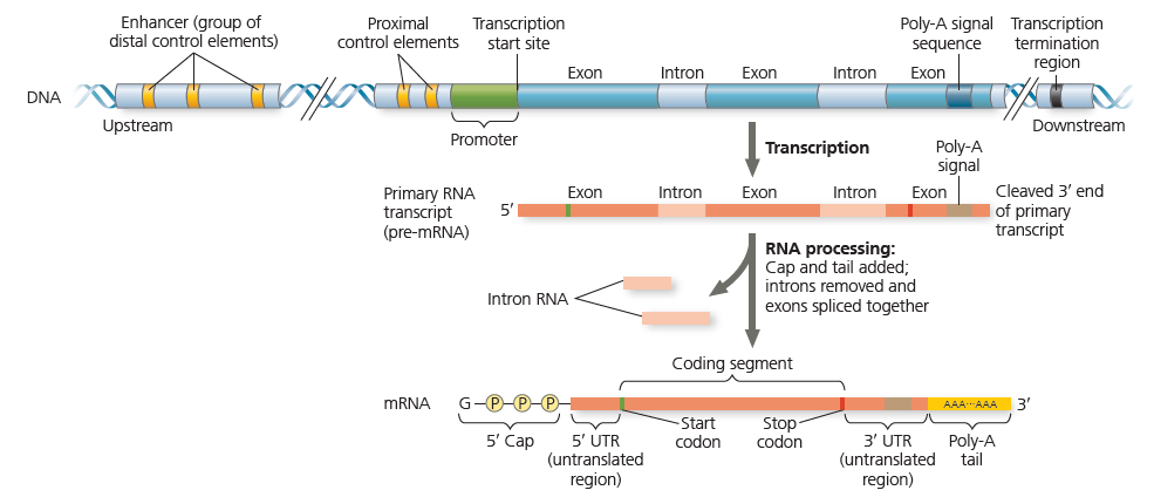
\includegraphics[width=\textwidth]{figures/from-DNA-to-RNA.png}
     \captionsetup{singlelinecheck=off}
    \caption[An eukaryotic gene and its transcript.]{
    This figure is reproduced from ~\autocite[Fig.~18.9, p.~373]{campbell_etal20}. 
    \begin{itemize}
        \item \textbf{Eukaryotic gene structure.} In addition to the coding sequence itself, each eukaryotic gene has a promoter, a DNA sequence where RNA polymerase binds and starts transcription. Control elements (in gold) \enquote{upstream} of both types, either close (proximal to) or far (distal to) from the initiation site, are involved in regulating the level of transcription. At the other end of the gene, a polyadenylation (poly-A) sequence signals roughly where the transcript is cleaved and the poly-A tail is added, while the RNA polymerase may proceed the transcription up to hundred of nucleotides further, stopping in the \emph{transcription termination region}. But the corresponding ribonucleotides are not added to the mRNA strand, and are rapidly degraded by enzymes instead.
        \item \textbf{Pre-mature RN.} Enzymes modify the two ends of a eukaryotic premRNA by the addition of the 5' cap and poly-A tail. The modified ends enable to export the mRNA to the cytoplasm, protect it from degradation and promote ribosome attachment during the protein synthesis phase. The 5' cap and poly-A tail are not translated into protein, nor are the 5' and 3' untranslated regions. The pink parts are the introns, sequences of RNA that are removed of the final mRNA strand, while the exons, the red parts, remain.
        \item \textbf{Mature mRNA.} During RNA processing, the introns are cut out and the exons spliced together. In many genes, the introns are much longer than the exons. (The UTR regions, while not coding for proteins, are considered exons because they remain in the final mRNA strand.) In the cell, some of these processes act simultaneously, addition of the 5' cap and splicing occurs while transcription is still under way.
    \end{itemize}}
    \label{fig:from-DNA-to-RNA}
\end{figure}


\subsection{Translation}
Translation is the process of synthesising a protein molecule from a RNA blueprint, driven by ribosomes (\enquote{protein complex} mixed with ribosomal RNA). It converts codons (triplets of adjacent nucleotides) of mRNA into the corresponding amino acids, the joined polypeptide sequence of them forming a protein.  

The process of translation can be divided into three main stages: initiation, elongation, and termination.
\begin{enumerate}
    \item Translation begins with the binding of the ribosome to the mRNA at \emph{the start codon} AUG, coding for methionine. Binding is facilitated by \emph{initiation factors}.
    \item The ribosome moves along the mRNA, adding amino acids to the growing polypeptide chain in the order specified by the genetic code. The \enquote{genetic code} relates the RNA sequence to the amino acid sequence in proteins: there are in total $4^3=64$ possible sequences of 3 codons, however, only 20 amino-acids prevail in nature. This implies that distinct codons code for the same protein. Each amino acid is brought to the ribosome by a transfer RNA (tRNA) molecule.
    \item Translation terminates when the ribosome reaches one of the three \enquote{stop codons}, namely UAA, UAG, and UGA, acting as the end site of the polypeptide chain. The completed protein is then released from the ribosome.
\end{enumerate}

Defects in translation can result in the synthesis of non-functional or toxic proteins, leading to various diseases and disorders. Indeed, proteins are essential, complex molecules that perform a wide range of functions in the human body, intervening directly in most of the biomechanical processes: 

\begin{enumerate}[label=(\alph*)]
\item \textbf{Structural support:} They are the essential bricks of our architecture, including tendons, bones, and skin, whilst maintaining the cell envelope. While some are inactive, others have the ability to contract, enabling the contraction of muscle fibres, such as actin and myosin.
\item \textbf{Enzymes:} Some species of proteins catalyse biochemical reactions, speeding up reactions within cells.
\item \textbf{Transport:} Some carry essential metabolites in vital fluids of the human organism, such as blood or lymph liquids. For instance, hemoglobin is in charge with the transport of oxygen in the blood towards the organs. 
\item \textbf{Cell signalling:} They convey essential signals among cells, enabling efficient communication in remote tissues. This ranges from hormones that regulate the \gls{metabolism} and control various physiological processes, such as insulin or adrenaline, to signal \gls{transduction}.
\item \textbf{Antibodies:} they intervene in the adaptive immune system by recognising and neutralising specifically foreign invaders.
\item \textbf{Storage:} Proteins such as ovalbumin are a renewed source of amino acids for building up other proteins.
\item \textbf{DNA replication and repair:} helicases and polymerases intervene in DNA replication, transcription and repair.
\end{enumerate}

Both the linear arrangement of amino acids in the protein sequence and its three-dimensional arrangement, commonly referred to as \Glspl{protein-structure}, often separated into four scales for clarity, play a crucial role to the final biological function of the protein. It is also important to note that not all proteins possess this intricate complexity, some being merely described at the single polypeptide sequence, and that modifications at any level of protein organisation can significantly affect its operational organisation, leading potentially to severe metabolic disorders. \Cref{fig:from-DNA-to-protein} illustrates the stages involved in synthesising a functional protein from a DNA sequence. 

\begin{figure}[p]
     \centering
     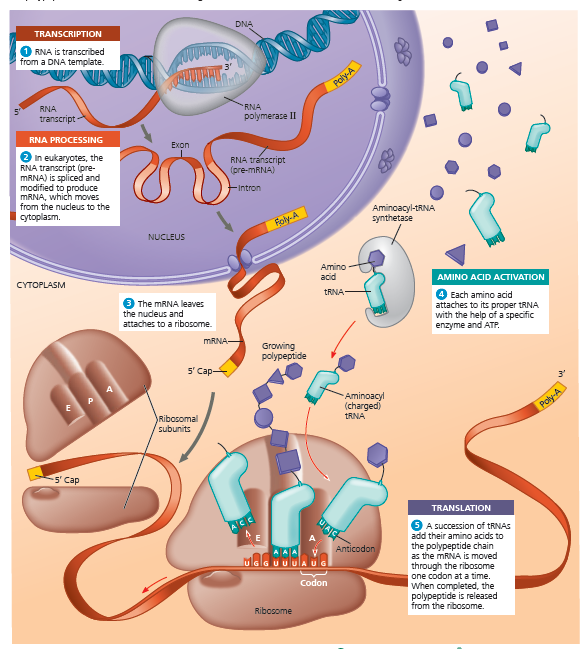
\includegraphics[width=\textwidth]{figures/from-DNA-to-protein.png}
    \caption[A schematic view of the process involved in protein production from an eukaryotic gene.]{
    This figure is reproduced from ~\autocite[Fig.~17.25, p.~356]{campbell_etal20}. Each gene in the DNA can be transcribed into several RNA molecules, and each mRNA can be translated to several proteins.}
    \label{fig:from-DNA-to-protein}
\end{figure}


\section{Regulation of gene expression}
\label{sec:gene-regulation}
\paragraph{Overview: coordinate the gene interactions:}
Just before the starting of concert, members of the orchestra individually tune their instruments in a gleeful but disordered cacophony. However, as soon as the conductor’s baton rises, all instruments join in to raise or lower their volume and their pitch at properly timing. And the original discordant sounds switch into a beautiful symphony that enraptures the audience.

In a similar way, cells must precisely regulate and coordinate their gene expression. Indeed, each cell type contains the same genetic material, however, by expressing a different subset of genes in a specific schedule, they are able to adjust to varying environmental conditions, to perform completely distinct actions, to pursue different biological roles and to fit to the growth development of the individual. Without this fine tune of gene regulation, how could we explain the complete distinct role played by a neuronal and a pancreatic cell? And how a fully developed human body emerges from a single egg cell, passing through the embryonic, foetal and adulescent stages? In the following sections we provide an overview of the \emph{regulation mechanisms} occurring in cells,  namely the way in which different genes are turned on and off at the right time. Gene regulation, as we will see, can occur in any stage of the gene expression process.

\subsection{Regulation of the chromatin structure}
Firstly, the level of transcription is modulated by the availability of the initiation sites and by extension to the level of compactness of the chromatin fibre.  Recall from \Cref{subsec:DNA}  that the DNA of eukaryotic cells is packed with proteins in a \enquote{protein complex} known as chromatin, the basic unit of which is the nucleosome. Indeed, when histones and DNA are tightly bound in the chromatin fibre, they limit the access of the RNA polymerase to promoters. This phenomenon of dynamic modification of chromatin architecture is called \emph{chromatin remodelling}.


The regulation of gene expression with respect to the compactness of the chromatin structure is influenced by three factors: the location of a gene’s promoter relative to the initiation sites, the overall compactness of the chromatin structure, for instance, genes within the heterochromatin, a highly-condensed region remain unexpressed. Lastly, some chemical modifications catalysed by specific enzymes over the tails of the histones protruding outward from nucleosomes or the DNA sequence itself can influence locally the chromatin structure by modifying the tridimensional structure and the folding of the histone proteins. 

Reversible addition of methyl groups (-CH3) to amino acids in histone tails can promote the condensation of the chromatin, while addition of a phosphate group, namely \emph{phosphorylation},  or \emph{histone acytelation}, namely when acetyl groups attach to lysines, induce a looser structure of the chromatin. The \emph{histone code} hypothesis suggests that the specific combination and order of chemical modifications yields the final configuration of the chromatin, which in turn influences transcription.


While some enzymes interact chemically with the tails of histone proteins, \emph{DNA methylation} refers to the process performed by a different set of enzymes, methylating directly certain bases in the DNA itself. It generally occurs at CpG (Cytosine-phosphate-Guanine) sites, the regions of the DNA sequence where a guanine follows a cytosine. DNA methylation mechanisms play a critical roles in gene silencing by inducing the condensation of the chromatin. Notably, DNA methylation seems to be involved in the long-term inactivation of genes supposed to remain active only during the embryonic phase. In opposition to the reversible changes induced by histone methylation, it seems that the methylation patterns remain permanent, with highly-specialised cells keeping the methylation blueprint acquired during the developmental phase, a process named \emph{genomic imprinting}. 

\todo{def eukaryotic, add illustration of the complex structure of a gene and alternative splicing, heterochromatin and eurochromatin 330-379 Campbell 12}

\subsection{Regulation of transcription initiation}
\label{subsec:reg-transcript}
Chromatin-modifying enzymes provide the first initial regulation of the
gene expression by controlling the access of a region of the DNA either more. Once the promoter site is reachable, the initiation of transcription involves the recruitment of proteins, building a \emph{transcription initiation complex} \Cref{subsec:transcript}.

Among them, the RNA polymerase II transcribes the gene and synthesises it into a primary RNA transcript (pre-mRNA). However, appropriate binding and efficient transcription requires the combination of regulatory proteins called \emph{\Glspl{tf}} with their corresponding binding sites acting as control elements.  Together, \acrshort{tf} interplay to precisely achieve the fine-tune regulation of gene expression seen, either activating or inhibiting the transcription process.


We set apart two types of transcription factors:
\begin{itemize}
    \item \emph{General transcription factors:} They are required for the initiation of the transcription of all genes, by either binding to the TATA box, a sequence present in most promoters, to other \acrshort{tf} or to RNA polymerase. However, their presence only leads to a low rate of RNA production. 
    
\item \emph{Specific transcription factors}: Precise and specific production of a given gene involves another set of proteins, the so-called specific \acrshort{tf}. They recognise specific sequences of DNA, that might be located close to the promoter (\emph{proximal control elements} or may be distant up to thousands of nucleotides upstream or downstream, the \emph{distal control elements}. A group of control elements acting together to which a TF uniquely binds to is called an \emph{enhancer}. Interestingly, while a gene may be associated to several enhancers, whose availability varies over time, each enhancer is only associated with a gene. 

\acrshort{tf} can either act as activators or repressors, and bind to other \acrshort{tf} or the DNA sequence itself. In the last case, they display the same two structural elements: a \emph{DNA-binding domain} that binds to the corresponding DNA control elements and several \emph{activation domains} that ease or inhibit \GLS{ppi} networks and by extension the efficiency of the transcription. 
\end{itemize}

Amazingly, while up to \num{20000} genes must be regulated in a human cell, only a dozen distinct nucleotide sequences control the pairing between TF and the DNA sequence, each enhancer being composed
on average of about ten control elements. It is the particular combination of control elements that yields the one-way matching between the enhancer and its corresponding TF. 


\subsection{Post-transcriptional regulation}
\label{subsec:alternative-splicing}

Recall from \Cref{subsec:transcript} that the original strand of mRNA resulting the transcription is not yet mature, and undergoes a series of biochemical interactions modifying its properties. Among them, \emph{alternative splicing} is the most fundamental mechanism of post-transcriptional regulation. 

Indeed, while all the introns are removed, not all the exons, even though coding directly for a protein, are kept in the final mature mRNA. It enables the production of protein variants, \emph{isoform proteins}, starting from the same pre-mRNA, as illustrated with the troponin gene below \Cref{fig:alternative-splicing}. Thus, a single gene can achieve different functions in the cell by controlling the proportion of each isoform produced. In fact, alternative splicing is the most likely explanation until now ($90\%$ of human protein-coding genes undergo splicing) for the low number of human genes identified (around \num{20000}), similar to that of a soil worm (nematode) or a mustard plant. 

\begin{figure}
    \centering
    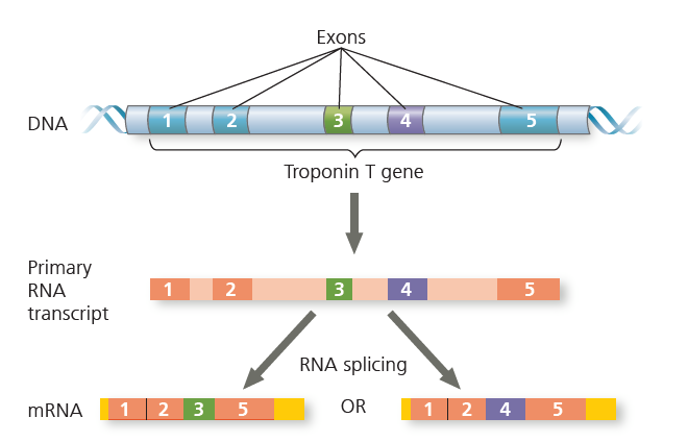
\includegraphics{figures/alternative-splicing.png}
    \caption[Alternative RNA splicing of the troponin T gene.]{This figure is reproduced from ~\autocite[Fig.~18.14, p.~378]{campbell_etal20}. Colour background of the exons are dark and introns light. The primary transcript of this gene can be spliced in several mRNA strands:  one ended up with exon 3 (in green) and the other with exon 4 (in purple). Both mRNAs are muscle proteins, differing slightly by their operational region.}
    \label{fig:alternative-splicing}
\end{figure}
Once the mature mRNA produced, it still must be translated into a protein. Conversion from a mRNA fragement to a functional protein highly depends on its average life span, which in return is related to the presence of translation regulatory proteins that recognise sequences of the 3 or 5' UTR(specific inhibition control, by preventing the binding of both RNA ends to the ribosome) or general effect protein factors, notably involved in development and differential phase. We display the mechanisms involved in ~\Cref{fig:model-enhancer}.

\begin{figure}
    \centering
    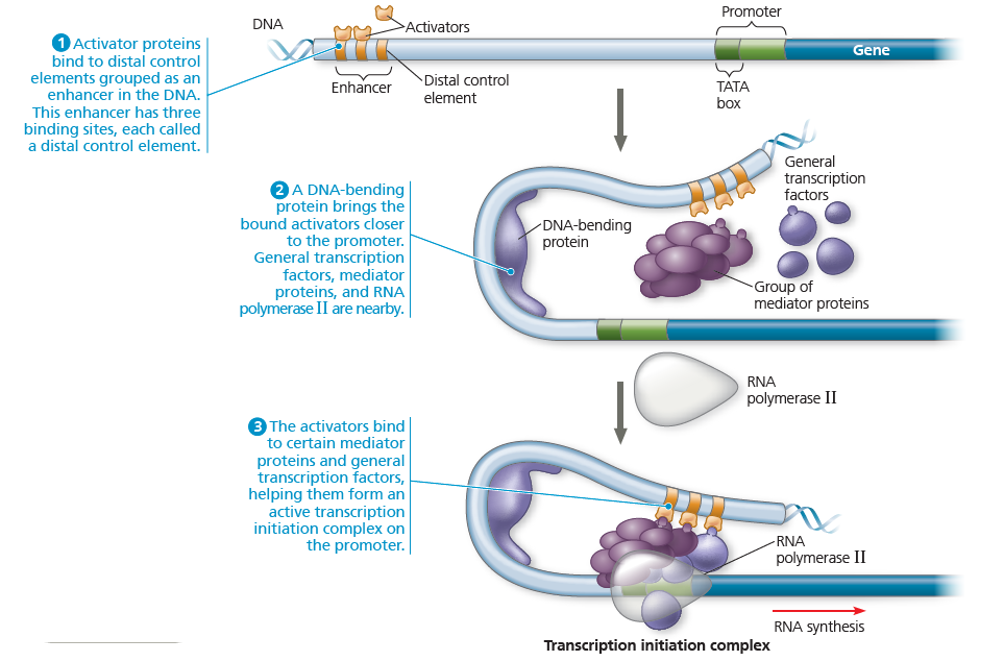
\includegraphics{figures/model-enhancer.png}
    \caption[\textbf{Model for the coordinate action of RNA polymerase and \acrshort{tf}.}]{This figure is reproduced from ~\autocite[Fig.~18.11, p.~375]{campbell_etal20}. The transcription initiation complex involves the coordinate binding of RNA polymerase II and general transcription factors, while fine-tune regulation is enabled by specific \acrshort{tf} that bind to the enhancers (here, represented with three control elements in gold) and to mediator proteins. It is DNA bending that enables enhancers to influence the regulation remotely. }
    \label{fig:model-enhancer}
\end{figure}


Interestingly, recent researches highlight the combined role of small non-coding RNAs (ncRNAs) molecules, known as microRNAs or miRNAs, and regulatory proteins in modulating gene activity. By base pairing to mRNAs, microRNAs mediate translational repression or the degradation of mRNAs. Other non-coding RNAs, including long intergenic ncRNAs (lincRNAs) or small interfering RNAs (siRNAs), seems to be involved but the associated regulation mechanism still needs to be deciphered. 

One of the first worldwide initiative related, to decipher the whole genome, is the ENCODE (Encyclopedia of DNA Elements) project, initiated in 2003: the main objective was to link a significant portion of the human genome to biological functions, encompassing protein-coding and non-coding genes. Another aspect of the program involved examining the associations between DNA sequence and histone tridimensional structures that influence the regulation of the gene expression(known as \enquote{epigenetic} alterations that impact gene expression while leaving the nucleotide sequence unaltered).Notably, this second phase involved more than 440 scientists in 32 research groups and 1,600 curated genomic experiences, and confirmed the high biological relevance of miRNAs while mitigating the wrongly acknowledged statement that most of the human genome was just \enquote{junk DNA}. Indeed, biochemical functions have been assigned to at least $80\%$ of the genome, $75\%$ of the human genome was found transcribed into functional RNA at some point whereas less than $2\%$ actually codes for proteins (\autocite{desouza12}, \autocite{ecker_etal12}, \autocite{gerstein_etal07} and \autocite{snyder_etal20}).


Complex biological functions require a coordinate set of chemical reactions, each with its own associated proteins, for instance the enzymes involved in a metabolic pathway or a transduction signal. As opposed to the solution developed in bacteria, in which genes involved in the same biological function are associated to the same promoter (\emph{operon} structure), genes that require co-expression are often scattered over the whole genome in human cells. In that case, coordinate control is triggered by \gls{cellular communication}, that in turn promote the recruitment of \acrshort{tf}. Since they move freely in the nucleus,  they are able to recognise and bind to the whole set of control elements.



\subsection{Post-translational regulation}
\label{subsec:post-transla}
Finally, post-translational modifications can occur at any time after the translation of the protein. By inducing chemical modifications to proteins, they alter its metabolic function or \emph{targeting}, a part of the protein sequence itself that addresses the final polypeptide sequence to its appropriate localisation. The most common modifications involve covalent additions of one or more side groups, including without intention of exhaustivity, phosphorylation, acylation, alkylation, and glycosylation. 

For instance, cell-surface proteins require membrane targeting and addition of sugars to get functional, while the insulin polypeptide proceeds from an original bigger precursor. 

Finally, the life span of each protein is strictly regulated by selective degradation. Giant protein complexes, the \emph{proteasomes}, recognise the ubiquitin-tagged proteins and degrade them. 


The several modifications discussed before do not entail a change in the DNA sequence, yet they may be transmitted to future generations of cells. The mechanisms involved in the inheritance of these specific traits is called \emph{epigenetic inheritance}, which in opposition to DNA mutations, are generally reversible. An increasing number of experiences confirm the importance of epigenetic may explain why only one of a pair of twins develops a genetically-based disease or the initiation of pro-tumoral conditions promoting the apparition of cancers. 

The control the epigenetic regulation mechanisms is itself modulated by the interactions between genes and the environment. Indeed, the degree of DNA methylation is thought to be related to the availability of nutrients. We display below a diagram summing up the biological mechanisms involved in gene regulation \Cref{fig:gene-regulation}.

\begin{figure}
    \centering
    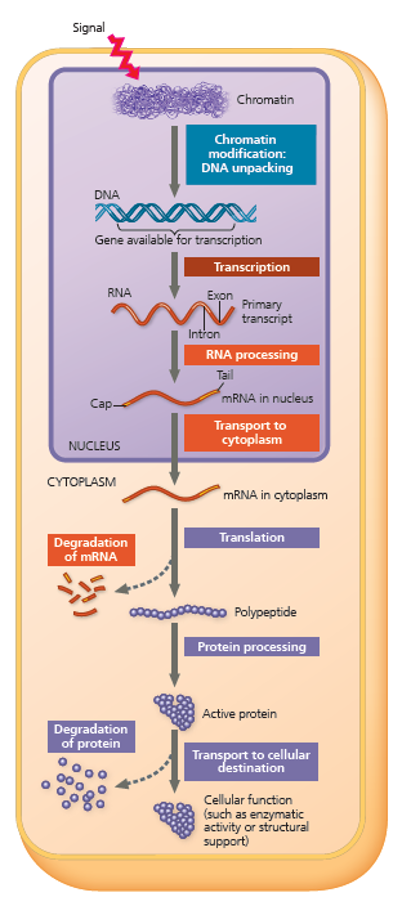
\includegraphics{figures/global-gene-regulation.png}
    \caption[The main gene regulation stages.]{This figure is reproduced from ~\autocite[Fig.~18.6, p.~370]{campbell_etal20}. In this diagram, each colour indicates the type of molecule regulated (blue = DNA, red or orange = RNA, purple = protein). Not all genes are regulated at all stages.}
    \label{fig:gene-regulation}
\end{figure}

\todo{autre figure, ou en GRN, à mettre ici, du stage de boolean}

It's worth noting that the entire regulatory machinery might not always be involved in the regulation of the production of specific gene. Furthermore, certain regulatory factors can operate on multiple levels: \acrfull{tf} can influence chromatin structure indirectly by recruiting proteins that acetylate histones to enhance transcription or directly by removing acetyl groups, resulting in transcriptional \emph{silencing} ~\autocite{walters_etal12}. More recently, new \emph{chromosome conformation capture} techniques reveal that entire regions within a chromosome (\emph{topologically associated domains}, or \emph{TADs}) bind into loops and congregate with each other, or with TADs from other chromosomes, to form sites associated with high transcriptional activity levels and often related to a given biological function. These \emph{transcription factories} are indeed rich in RNA polymerase and other \acrshort{tf}. 

In next section, we detail some sequencing tools that can be used to keep track of the variations of the transcriptome and help unravel the relations between the biological features. 

\section{Capture variations of the transcriptome}
\subsection{Overview: definition of the transcriptome:} 
\label{subsec:transcriptome-overview}
Among the several types of omics that can be analysed to unravel the relationships between the biological entities, wefocus on transcriptomics, the analytical study of the transcriptome, as it is certainly the kind of biological data for which the most technologies have been developed, and as it indirectly provide clues on the interaction between DNA and protein and how they contribute to the biochemical processes involved in keeping the organism in proper operating order. The transcriptome is simply the collection of all RNA molecules, types and quantity, present at a given time in a biological sample.  

While tools for quantifying gene expression levels have been developed for years, for a long time, they focused on a single gene at a time. Among them, the most widely used were Northern blots or Reverse Transcription-Polymerase Chain Reaction (\acrshort{rtpcr}) as well as sequence-based approaches such as Serial Analysis of Gene Expression (SAGE) or comparative Expressed Sequence Tag (EST). Nevertheless, all the technologies described above have in common the generation of a sequence of nucleotides complementary to the original material. Precisely, the specific mRNA sequence of interest is used as a template to synthesise a complementary, single-stranded RNA strand using nucleic acid hybridisation (recall from \Cref{subsec:DNA} that the two strands of DNA hold from base-pairing, with each nucleotide uniquely recognising another amino acid among a repertoire of four, property called \emph{hybridisation}). Each of these paired nucleotides, used as as a surrogate for the presence of the mRNA, is called a \emph{nucleic acid probe}. In addition, the pair original mRNA-cRNA or DNA is uniquely identified with a fluorescent tag, in a technique called \emph{in situ (\enquote{in place}) hybridisation.} (the total number of mRNAs that can be followed at the same time is however limited). 


As an example, we describe in few words the widely used \emph{reverse transcriptase polymerase chain reaction (\acrshort{rtpcr})} method. The first step consists of synthesising a double strand complementary DNA sequence, expunged of introns, by the combined use of reverse transcriptase and DNA polymerase with a RNAse enzyme in charge of degrading the original mRNA material. Indeed, RNA is reverse transcribed to cDNA since DNA is more stable and enables more efficient amplification and the use of mature DNA sequencing technology. Then follows an \emph{amplification stage} generating many copies of the RNA segment of interest: the PCR step, which notably requires \emph{primers}, short chemically synthesised oligonucleotides that initiate the replication by attaching the DNA polymerase in place. Finally, newer methods such as qRT-PCR (\emph{q} stands for \emph{quantitative}) enable precise quantification while avoiding the burdensome and time-consuming electrophoresis step.


However, it is generally much more interesting to capture \emph{simultaneously} the evolution of the mRNA levels between all the genes to better understand how they act in concert to perform complex biological functions. This new approach of the field is called the \emph{systematic approach}. For that reason, we focus on the technologies that enable to analyse the \emph{whole transcriptome} in a high-throughput manner, with, by chronological order, the apparition of microarray technologies, and then the development of Next-Generation Sequencing (\acrshort{ngs}) methods. Compared to microarray, \acrshort{ngs} technologies present the main advantage of not being restricted to already known documented DNA or RNA sequences. 

The principle and technology of microarrays and RNASeq methods are further detailed respectively in \Cref{subsec:microarray} and \Cref{subsec:RNASeq} from a molecular biologist and \gls{bioinformatic} point of view, namely from the data production workflow to the raw mapping of counts, without further normalisation. Promising technologies, that would enable to follow in real time the spatial and temporal evolution of transcriptomics, are mentioned in the last paragraph of this section \Cref{subsec:miscelleanous-innovative-rna-seq}. Note that these promising technologies would not have been possible without the global sequencing projects in late $20^\text{th}$ century, as most of them rely on a reference genome to align the investigated mRNAs. 

Finally, once we have collected the raw counts or arbitrary quantitative units (for microarray), we detail statistical methods in \Cref{chap:transcriptome-workflow} to address the challenges associated with this type of data, along with appropriate normalisation processes to apply these method. Transcriptome datasets find diverse biological applications, including \emph{differential analysis}, which aims to identify genes exhibiting significant differential expression between two distinct biological conditions (often involving comparisons between control/healthy and disease samples),  subgroup identification of patients sharing similar expression profiles, usually by performing \emph{clustering}-based methods and computation of the disease prognosis. These methods typically operate within a semi-supervised framework, often integrating prior medical knowledge with \emph{unsupervised} machine-learning techniques.


 \subsection{Microarray technology to quantify gene expression}
\label{subsec:microarray}
Microarray plates are small chips onto which tens of thousands oligonucleotide probes, with sequences complementary to fragments of actual genes, are engraved. Generally, each gene is normally represented by a set of probes, so called a \emph{probeset}, each representing a different but highly-specific gene region. Indeed, designing customised probes reveals a painstaking task, as the challenge is to identify a combination of nucleotides both characteristic of our coding gene and not matching any other genome region, with the risk of detecting a spurious pairing otherwise. In addition, due to natural limitations of sequencing technologies, the length of the complementary probe is thus generally between 25 bp and 60 bp long.  

The following protocol is common to most of the microarray technologies:
\begin{enumerate}
    \item The mRNA samples, called the \enquote{targets}, are extracted from the investigated biological sample. 
    \item The targets hybridise to their complementary probe on the microarray and are labelled using fluorescence or radioactive labels. 
    \item Two competitive methods are used to compare gene expression levels between two biological conditions, as presented in \Cref{subfig:one-vs-two-channel}. Either the two mRNA preparations are hybridised at the same time, the RNA strands competing for the access to the probes, or each sample is assigned its own array, but with the same dying label (an extensive comparison of the pros and perks of both approaches is reviewed in \autocite{patterson_etal06}, \autocite{kuo_etal06}, \autocite{severgnini_etal06} and \autocite{sirbu_etal12}). In both cases, each probe is generally duplicated thousands of time in the same \enquote{probe cell} (see \Cref{subfig:probe-structure} for details), called a \emph{spot}, to trap the target mRNA fragment.
    \item Once the hybridisation step is performed, high-spatial resolution pictures of the plate are carried out, on which a spot is likely to be represented by many pixels. The \emph{segmentation} stage sets apart pixels proceeding from a spot, marked as relevant signal, from pixels out, marked as background noise. Finally, the \emph{quantification} stage itself aggregates the individual intensity values of a spot into an unique signal, used as proxy of the abundance of mRNA and reports them in files with CEL extension.
\end{enumerate}

\begin{figure}
     \centering
     \begin{subfigure}[p]{0.2\textwidth}
         \centering
         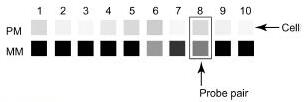
\includegraphics[width=\textwidth]{figures/biological_introduction/probe_structure.jpg}
         \label{subfig:probe-structure}
         \caption[\textbf{Probe set structure}]{A micro-array chip is composed of a huge collection of probe oligonucleotides whose sequence is complementary to RNA targets. 
         To enhance detection power and assess variability, the probes are further organised into \textit{probe sets}:  a collection of perfect match probes (PM) that precisely match the target sequence paired with mismatch probes (MM) that only differ by a single base mismatch.
         Hereby, we can assert the specificity of each probe by quantifying the relative binding of the target sequence between the PM and MM probe. 
         The collection of probes is stored in a CDF file and the related value in a CEL file, each of them being uniquely identified by an affyID, figure reproduced from \href{https://www.affymetrix.com/support/downloads/manuals/chas_2_1_user_manual.pdf}{Affymetrix technical manual}.}
     \end{subfigure}
     \hfill
     \begin{subfigure}[p]{0.55\textwidth}
         \centering
         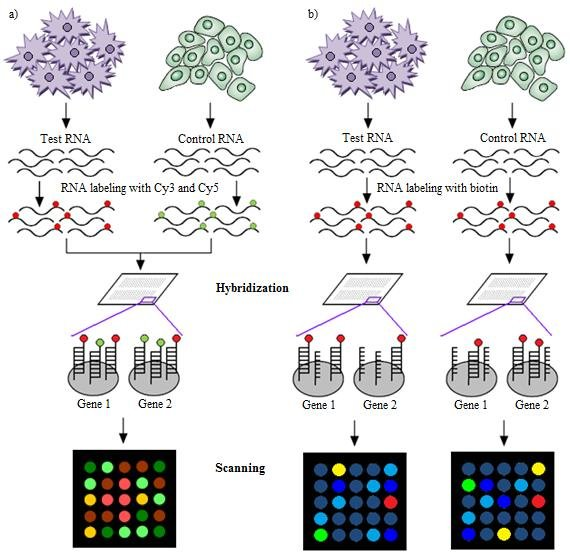
\includegraphics[width=\textwidth]{figures/biological_introduction/Microarray-Hybridization-using-a-two-channel-and-b-single-channel-microarray.png}
         \label{subfig:one-vs-two-channel}
         \caption[\textbf{a) Two-channel and b) Single-channel microarray platforms}]{This infographic (reproduced from \autocite[Fig. 6]{dawany23}) illustrates the technical protocol differences between single-channel and two-channel microarray technologies. Briefly, one-colour channel Microarray uses a single fluorophore to quantify the relative signal intensity of a disease sample against a common reference (generally a control, healthy case-control) and exhibits simpler experimental design. On the contrary, two-colour channel Microarray methodology is based on two different fluorophores (often Cy3 and Cy5) to compare directly two samples within the same microarray slide, hereby offering enhanced sensitivity to detect differential gene expression in comparative analyses.}
     \end{subfigure}
   \caption[A brief overview of micro-array chips to quantify the transcriptome]{}
    \label{fig:microarray-technology}
\end{figure}

Although generally neglected nowadays against \acrshort{ngs} technologies, new promising microarray applications continue to emerge, ranging from \acrshort{snp} detection to copy number variations through identification of methylated regions or protein binding sites. Notably, their extreme high miniaturisation makes them the best compromise between the requirement of high-throughput and cost-saving technologies, one of the most widely used technology being the \href{https://www.affymetrix.com/support/downloads/manuals/chas_2_1_user_manual.pdf}{Affymetrix} suite \footnote{For instance, the Human Genome U133 Plus 2.0 Array (HGu133+, released by the Affymetrix company) gathers \num{54000} probesets, spotted by 11 different probes, comprising overall more than \num{1300000} distinct oligonucleotide sites.}, with a bunch of dedicated R packages and methods to aggregate probesets into an unique gene expression measure while discarding background noise or accounting for specific bias (\autocite{gautier_etal04}, \autocite{irizarry_etal03}).


\subsection{RNASeq technology}
\label{subsec:RNASeq}
\acrfull{ngs} methods are cutting-edge technologies, emerging from early 2000's, that bridge the gap between the high-throughput sequencing capacity of microarray technologies and the versatility of traditional sequencing methods which can build from scratch an unknown genome. Numerous sequencing methods have been developed, with different biological applications and limitations. We generally identify three sequencing generations, differing by the nature of the reads generated (either short or long, direct RN or requiring prior conversion to cDNA) and the sequencing throughput.


First-gen(eration) \glspl{sequencer}, like the ABI capillary technology, offer high accuracy and longer read lengths, but lack high-throughput sequencing. Second-gen platforms (e.g., Illumina's MiSeq, HiSeq, NextSeq and Thermo Fisher Scientific's Ion Torrent) achieve both high throughput and accurate \emph{base-calling} via parallel sequencing. However, their shorter read lengths pose challenges in assembling repetitive sequences. In contrast, third-gen sequencers (e.g., Pacific Biosciences' PacBio, Oxford Nanopore Technologies' MinION, PromethION, SmidgION) generate long reads at high throughput by sequencing single-molecule, at the expense of a higher error rate. In this section, we focus on the Illumina sequencing technology since all the datasets used for our analysis were sequenced through this platform \footnote{Going further,it is up to $90\%$ of all DNA sequenced data that were generated with the Illumina platform, from estimations reported in \href{https://emea.illumina.com/techniques/sequencing/rna-sequencing/total-rna-seq.html}{Illumina leaflet}, in 2015.}, which is not surprising since the human genome is well annotated and we were only interested in our downstream analyses in comparing transcriptomic profiles at the gene level, not the isoform one, across thousands of biological samples. However, the interested reader may report to glossary keys \glspl{sequencer} for a comprehensive review of sequencing techniques and \glspl{library} for an overview of biological applications with respect to the nature of the generated reads. \autocite{slatko_etal18} describes generation after generation the mere principles underlying each technological breakthrough along with a collection of useful papers and web links for each sequencing platform, and \autocite{vilgis_deigner18} is a book chapter addressed specifically for practitioners of precision medicine. Ultimately, \autocite{lam_etal12} and \autocite{cottrell18} are essays reviewing quantitatively several RNASeq methods, while proposing further possible evolution perspectives for these technologies.


Hence, while the final choice of the sequencing platform choice depends on the biological application and the human expertise and financial resources available, all of them present the following four stages in their workflow sequencing pipeline, summarised in \Cref{fig:rna-seq-workflow}:

\begin{enumerate}[label=(\roman*)]
    \item \textbf{Library preparation:} The transcriptome of the sample or tissue of interest, after an isolation stage, is reverse-transcribed into \gls{cDNA} for stability purposes. The next step consists of randomly fragmenting cDNA into strands of smaller sizes, called \emph{inserts}, and ligating two distinct adaptors, one at each end, in a process called \enquote{tagmentation}. The set of obtained cDNA fragments is termed the \enquote{library} (see also subfigure a, in \Cref{fig:rna-seq-workflow}).
    
    \item \textbf{DNA amplification:} Compared to old-fashioned sequencing methods, \acrshort{ngs} technologies mostly differ by their higher capacity of DNA amplification and sequencing. After an initial amplification stage, employing similar techniques to \acrfull{rtpcr}, comes the \emph{clonal amplification} stage itself in order to increase by several orders of magnitude the total amount of DNA available for sequencing, compared to more traditional approaches (note that this prior amplification stage is mostly required for sequencing methods that do not sequence directly RNASeq, but rather convert it first into cDNA, as reviewed in \Cref{subfig:library-comparison-preparation}). Here, the DNA amplification process largely differs between platforms, thus we restrain to the study of the \Gls{illumina} protocol. Precisely, the clonal amplification stage mitigates the lower sequencing quality inherent to \acrshort{ngs} in comparison to conventional methods, while achieving a significantly stronger genome coverage \footnote{Up to 180 million reads are generated by the HiSeq 2000 platform}. This is particularly valuable for sequencing challenging regions of the genome, including repetitive segments, GC-rich regions and \emph{homopolymers}, which tend to pose accuracy hurdles during sequencing.
    
    The initial Illumina amplification relies on a lawn of oligonucleotides, complementary to the sequences of the adaptors, which are attached to a glass surface, called a \emph{flow cell} and composed of thousands of \emph{tiles}. In parallel, the DNA library is \emph{denatured} to form single-stranded DNA (ssDNA) fragments which subsequently tether to the surface-bound oligonucleotides.
     Next, the so-called amplification stage relies on a process called \enquote{bridge amplification}, in which each hybridised fragment is cloned separately and simultaneously into $\approx 1000$ copies, forming a \emph{cluster}. This process is enabled by the two types of oligonucleotides bound to the flow cell: they indeed allow alternated synthesis in both directions of the cDNA fragments, a process repeated until the desired amount of DNA has been reached (see also subfigure b, in \Cref{fig:rna-seq-workflow}). 
    
    \item \textbf{Sequencing:} Genome sequencing consist of determining the sequence of nucleotides of the whole set of fragments composing the DNA library and the technique is itself highly dependant on the platform used. The resulting data output is typically stored in \Gls{FASTA} or FASTQ files.
    
    Again, we focus on the Illumina high-throughput and massively parallel sequencing protocol. Briefly, fast sequencing of fragments rely on a proprietary reversible \enquote{terminator} method that detects single addition of bases in the mean time they are incorporated. Specifically, each sequencing cycle starts with the addition of a primer and fluorescent reversible-terminator nucleotide (rt-dNTPs), ensuring that only one nucleotide is added at a time. Any unbound nucleotide is then washed away, while lasers excite the fluorescent tags of each incorporated nucleotide, each being associated to its own wavelength. Finally, the tag is cleaved off, putting an end to the cycle. This procedure, known as \enquote{sequencing-by-synthesis} is iteratively performed until the desired sequence length is achieved. The number of cycles employed dictates the resulting sequence length, a balanced trade-off between generating overly brief strands that might yield ambiguous mapping information in the subsequent assembly stage, and overly extended ones that carry an elevated risk of compromised synthesis quality at the 3' end. 
    The resulting images are then processed to return the \emph{reads} themselves (the string sequence, each character coding for one of the four RNA nucleotides). To achieve this, the nucleotide identification process computes the signal intensity and noise for each of the identified cluster, in every set of raw image files generated during the \enquote{sequencing-by-synthesis} phase. This transformation of raw intensities into interpretable reads encompasses tasks such as background noise correction, accurate cluster identification, and determination of scaling intensity. This multifaceted procedure is referred to as \emph{base-calling} (see also \autocite{illumina23} for an industrial overview or \autocite{raghavendra_pullaiah18} and \autocite{meyer_kircher10} for a didactic and unbiased academic point of view).
    Better sequencing quality can be further achieved by synthesising fragments in both directions of each cDNA sequence, as illustrated in \autocite[Figure 4: Paired End Sequencing]{illumina23}. The resulting \enquote{paired-end} library has twice the number of reads for the same dedicated efforts, increasing the quality of the alignment and providing refined opportunities for the detection of \enquote{indels} (insertion deletion modifications), \acrshort{snv} and \acrshort{snp} mutations (see also subfigure c, in \Cref{fig:rna-seq-workflow}).        
    
    \item \textbf{Alignment and assembly:}  From the billions of reads sequenced, computer software and bioinformatic tools rebuild the whole transcriptome, by locating each read in the genome. Two strategies are used, depending on the level of prior information available: \emph{de-novo} strategy, as its name suggests, refers to construction of genomes when no annotations are available while the \emph{genome-guided} strategy aligns and maps reads onto a genome of reference.     
    \emph{De-novo alignment} is a highly-challenging task, especially for covering highly repetitive regions of the genome, while early errors performed at this stage can drastically reduce the performance of downstream analyses, notably the methods targeting genomic events, such as chromosomic rearrangements, \acrfull{snp} or even indels (for inserts and deletions). However, such issues can be alleviated by coupling short-read assembly with long-read paired-end sequencing information. This strategy, known as \glspl{genomic-scaffolding} involves generally an intermediate step which consists of generating larger individual \glspl{contig} before the final reconstruction of the whole genome. And \autocite{luo_etal21} (a comprehensive state-of-the-art review of scaffolding methods in genome assembly), \autocite{rice_green19} and \autocite{sohn_nam18} (provides guidelines for determining the optimal approach based on input data and computational budget, providing an optimised use from long reads to overcome the limitations of short reads) established that the optimal sequencing quality and coverage are achieved by combining reads of diverse sizes: shorter ones derived from \acrshort{ngs} and longer inserts obtained through traditional sequencing methods, generally with lower read depth.
    
    We now focus on the \emph{reference-based strategy}, generally favoured for human genome assembly since it has already been reconstructed globally in the early 2000's. While historically, the literature corpus focused on alignment methods for long reads generated through conventional sequencing, such as the renowned BLAST \autocite{altschul_etal90},  such methods are unsuitable for aligning the short reads returned by \acrshort{ngs} technologies nor pairing fragmented and discontinuous RNA fragments (remember from \Cref{subsec:transcript} that certain parts of the original DNA sequence are discarded in mature mRNA, including all \emph{introns}, or split into several parts). Lastly, short reads with repetitive patterns have an equal chance of aligning to various distant regions of the genome, as discussed in \autocite{treangen_salzberg12}.
     Hence, numerous alignment bioinformatic tools, designed specifically to address this short-sized issue and review in \autocite{treangen_salzberg12}, have been developed since then. Notably, to deal with alternative splicing (\Cref{subsec:alternative-splicing}), most of these methods proceed shorter portions of the read, named \endquote{seeds}, through dynamic programming, in order to find the alignment with the most overlapping sequences (among developed mapping algorithms, the most popular are BowTie2 \autocite{langmead_salzberg12}, TopHat2 \autocite{kim_etal13}, STAR \autocite{dobin_etal13} and HISAT2 \autocite{kim_etal19}). The final output is a BAM file, which can be interpreted as a global map of the genome, in which each read is associated a unique pair of \enquote{genomic spatial coordinates}. We also denote the final number of reads identified and mapped to the genome as the \emph{library size} or \emph{sequencing depth} (see also subfigure d, in \Cref{fig:rna-seq-workflow}).  
     
     \autocite{srivastava_etal20} benchmarks a huge collection of alignment and mapping methods to determine their impact on the estimation of transcript abundance estimation. They observe significantly different and variable performance between lightweight-mapping and more traditional alignment-based methods. They tried to elucidate this diversity by examining a bench of factors, and observe notably that performing spliced alignment to the genome and then projecting these alignments to transcriptome provides better mapping performance compared to directly aligning to the transcriptome.
    
    \item \textbf{Quantification:} Once all reads are aligned to a reference genome, the final stage of the RNA-seq processing workflows involves the estimation of transcript abundances, generally under the form of raw count measures at the gene or transcript isoform level. Primarily, only the reads overlapping perfectly a given exon of the original genome sequence were annotated, for instance consider HTSeq \autocite{anders_etal15} and FeatureCounts \autocite{liao_etal14} tools. Since then, advanced methods that are particularly effective with limited annotation information involve a preliminary construction of \glspl{contig}, enabling to rebuild from scratch newly unobserved transcript variants by including junction reads and unannotated transcripts (see for instance Cufflinks \autocite{trapnell_etal10} or StringTie \autocite{pertea_etal15} tools). Ultimately, Kallisto \autocite{bray_etal16} and Salmon \autocite{patro_etal17}, an updated version that accounts for sample-specific technical bias such as fragment GC-content or positional bias, are both lightweight methods relying both on a probabilistic framework and the identification of \glspl{kmer} regions, to make the alignment methods more scalable and accurate. Hence, they both stand out as cutting-edge methodologies by achieving similar accuracy to predecessors while being significantly faster (around 2 orders of magnitude, see also \href{https://gencore.bio.nyu.edu/salmon-kallisto-rapid-transcript-quantification-for-rna-seq-data}{Salmon and Kallisto: Rapid Transcript Quantification} for a practical implementation through R programming).
    
\end{enumerate}

\begin{figure}[p]
     \centering
     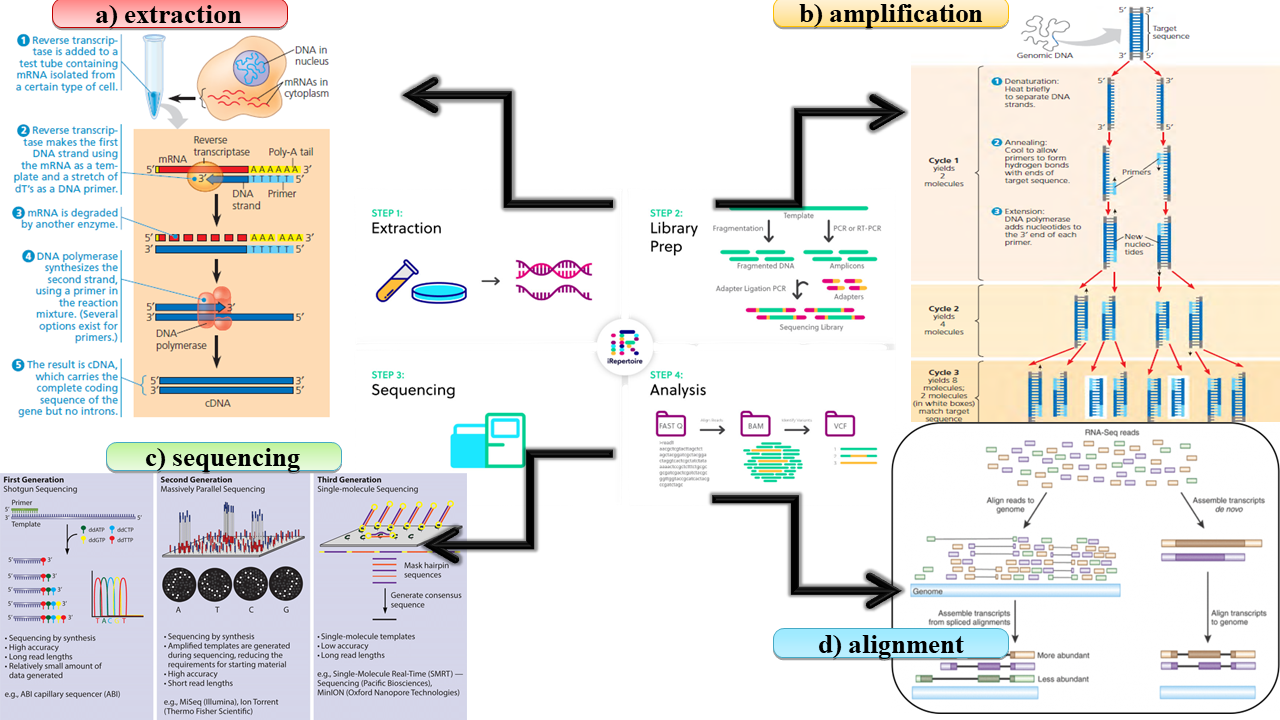
\includegraphics[width=0.95\textwidth]{figures/biological_introduction/general_workflow_pipeline.png}
     
   \caption[\textbf{Next generation sequencing (NGS) workflow:}]{
   The entire NGS workflow can be broken down into four steps: 
   \begin{enumerate}[label=\emph{\alph*})]
       \item \textit{Sample extraction:} When RNA is the starting template, an additional step, between the RNA extraction, and the library preparation itself, is required to convert the RNA into c(omplementary)DNA by reverse transcription (reproduced from \autocite[Fig 20.10]{campbell_etal20}).
       \item \textit{Library preparation:} Preparation of a sequencing library typically involves two steps: 1) \textit{RNA amplification} to increase the amount of appropriately sized target sequences and 2) the addition of \textit{adapters} to uniquely identify them. PCR (for polymerase chain reaction) is one of these techniques to copy many times any target
       sequence within a test tube, which only requires double-stranded DNA containing the target
sequence, a heat-resistant DNA polymerase, all four nucleotides, and two single DNA strands that serve as primers, one for each end of the target sequence (reproduced from \autocite[Fig 20.7]{campbell_etal20}).
       \item \textit{Sequencing RNA library:} Currently, we generally classify all sequencing platforms into three generations, each coming with distinct strengths and weaknesses (subfigure c reproduced from \autocite[Fig .1]{ronholm_etal16}).
       \item \textit{RNASeq analysis: } when studying an organism with a reference genome, it is possible to directly map the reads onto the reference transcriptome \footnotemark{1}. However, without a reference organism, the individual genome must be constructed from scratch: \enquote{de-novo assembly}, see key \gls{contig} and \gls{genomic-scaffolding} for details (subfigure d reproduced from \autocite[Fig. 1]{ronholm_etal16}).
   \end{enumerate}   
   The general framework of this illustration is reproduced from \autocite[Fig. 1]{g20}.}
    \label{fig:rna-seq-workflow}
\end{figure}

\footnotetext{Mapping reads directly to the genome presents the fundamental advantage of not knowing the exact way exons are spliced, hereby allowing the discovery of unknown variant transcripts issued from alternative splicing (see \Cref{subsec:reg-transcript}.}


The final quantification stage is used in a number of downstream analyses (see \Cref{sec:downstream-analyses}) to study dysregulated biological mechanisms and retrieve biomarkers characteristic of diseases, and may be used as well as proxy of the proteomic level, although much precaution is required due to post-transcriptional events, see \Cref{subsec:post-transla}, \Cref{sec:patrimony-overview} and paper \autocite{meissner_etal13} for limitations of RNASeq use as an intermediate measure for the proteome). 
In addition, while RNASeq enables to consistently compare ratios of transcript levels across two biological conditions sampled with the same sequencing platform, even raw counts do not correspond exactly to the absolute levels of gene expression, since this value depends on the sequencing depth (see \textbf{alignment} bullet point before), an issue partially mitigated with \Glspl{spike-in} normalisation (consider for instance the R implementation of a spike-in normalisation technique in Bioconductor package \texttt{BRGenomics} \autocite{deberardine23}.


Overall, various factors justify the increasingly prevalence of RNA-seq based technologies over microarray ones. Firstly, it does not rely on hybridization with a labelled probe, hence an annotated or reference genome is not anymore a prerequisite \autocite{wang_etal09}. Hence, relying solely on the transcripts bound to the array chips, Microarrays require good annotation for the model organism’s transcriptome, and can not capture genomic or transcriptomic individual events, such as mutated RNA or unknown alternative spliced transcript, since the mutated sequence differs from its complementary probe and hereby, is likely not to bind to it. Secondly, it can cover expression levels over a much broader range: while microarray technologies provide a continuous signal with limited detection range (background noise for low expression levels and saturation at the high end), RNA-seq inherently provides discretised measurements, quantifying gene expression as non-negative integer counts \autocite{wilhelm_landry09}. Thirdly, the versatility of RNA-seq technologies opens up new research areas, including the detection of alternative splicing isoforms and specific mutation disorders, from standard to \acrshort{snp} to more delicate general transcript fusion events \autocite{mantione_etal14} (specific benchmarking of RNA-seq based technologies, relying on concordance correlation with RT-qPCR expression data, is proposed in \autocite{everaert_etal17}. 

Precisely, \autocite{guo_etal13} observed that low abundant genes had poorer correlations between microarray and RNAseq data compared to high abundance genes, especially the Agilent two-channel microarray, with Spearman correlation of only 0.2 in TCGA datasets. Interestingly, \autocite{zhang_etal15} shows that RNA-seq outperformed microarrays in determining the transcriptomic characteristics of cancer (the studied cohort included 498 neuroblastoma patients), while both models performed similarly in clinical endpoint prediction (see also  \autocite{xu_etal13} for a more limited benchmark study comparing solely Illumina RNA-Seq and Affymetrix microarray platforms' performance). Confirming empirically these specific clinical examples, the meta-review \autocite{malone_oliver11} and opinion paper \autocite{mantione_etal14} confirm the utility of microarrays, notably as being more cost-effective and reliable for gene expression profiling in model organisms; yet, both approaches exhibit a strong congruence when asked the same biological question. 
Going further, \Cref{subsec:miscelleanous-innovative-rna-seq} summarises new RNA-Seq perspectives, notably to examine intricate transcriptome fine structure, such as allele-specific expression and isoform identification.

\subsection{Perspectives: single cell and spatial transcriptomics}
\label{subsec:single-cell-spatial-transcript}


\paragraph{Limitations of \acrshort{RNA-Seq} technologies}

As reviewed in \Cref{subsec:miscelleanous-innovative-rna-seq} and \Cref{subsec:RNA-Seq}, the ability of \acrshort{RNA-Seq} technologies to perform high-throughput sequencing analysis and sample multiplexing gives new insights on biological mechanisms. However, they are tailored to dissect bulk mixtures mixing different biological entities, preventing from deciphering complex biological mechanisms proceeding from interactions between distinct biological entities. Additionally, \acrshort{RNA-Seq} outcomes are simply snapshots of the current transcriptome state at a given time, without precise temporal or spatial annotation. Thus, they can not be used to understand sub-cellular mechanisms or interactions occurring between distinct biological compartments. Ultimately, the preparation of the RNA library is a destructive process, involving degradation of the cell membranes to extract the \acrshort{RNA-Seq} reads.

\subsubsection{Single-cell RNASeq technologies}
\label{subsec:sc-rnaseq}

\acrshort{scrna} technologies deal with two main specific challenges: the isolation of individual cells and the amplification of minute amounts of RNA.  

Advancement of techniques for reducing the cost and the human burden of separating individual cells, even those intricately embedded within tissues, has been ongoing \autocite{fan_etal15}. They hence evolved from historical, low-throughput methods that relied on manual isolation of individual cells, hereby limiting the analysis to a few dozen cells \footnote{Such methods encompassed micromanipulation \autocite{tang_etal09} and laser capture microdissection (LCM) techniques \autocite{gautam_etal21}.}. In contrast, modern approaches involve high-throughput automated dissection and sorting of tissues, made possible through techniques such as microdroplets \autocite{bageritz_raddi19} and microfluidics \autocite{sarma_etal19}.

The sequencing and amplification of \acrshort{RNA-Seq} implies the same stages as standard \acrshort{RNA-Seq} methods, namely (1) reverse transcription, (2) cDNA amplification with PCR, for an exponential amplification, or in vitro hybridisation, for a linear amplification, and (3) the sequencing of the library itself, see \Cref{subfig:sc-pipeline} and \Cref{subsec:RNASeq}. Capturing small amounts of DNA is a challenging task:  \autocite{islam_etal14} hence observes that only $10\%$ in average of all transcripts get reverse transcribed, implying systematic underestimation of the level of expression lowly expressed genes. In addition, the amplification pattern can be relatively tedious to capture, leading to a systematic bias when interpreting the estimated expression levels of RNA (as described in \Cref{subsec:RNASeq}, this aspect can be alleviated by using \glspl{spike-in} normalisation combined with the use of UMI (unique molecular identifiers) to barcode and retrieve easily the origin of each individual mRNA read). 

Ultimately, the inherent sparsity of the RNA library and the intricate protocol of \acrshort{scrna} technologies make them susceptible to significant technical biases. Additionally, the vast amount of data generated requires the use of efficient storage and analytical tools. 
A set of bioinformatics methods, still under active development, make this type of data interpretive, enumerated in \Cref{subfig:sc-nextflow}. First, they are used to assert the quality of the library, discarding cell doublets, dead cells or samples without any cell captured, evaluating the level of degradation of the mRNA (for instance, by controlling the expression level of \emph{endogenous, housekeeping} genes \autocite{shalek_etal14}), controlling a posteriori the distribution of the read lengths, removing aberrant samples that should not be wrongly confused with rare cell type phenotypes, \ldots
 

The high resolution of \acrshort{scrna} technologies allows a better understanding of complex biological pathways, which were not accessible to standard methods of bulk cell population profiling. Notably, they can be used to finely characterise subpopulations within a sample by identifying specific \gls{cell marker}, driver genes involved at key developmental stages, differential splicing and allelic expression patterns between populations, \ldots In turn, combining these information reveal useful to infer gene-regulatory networks and \emph{pseudo-time analysis}, giving insights on holistic, dynamic mechanisms of the biological systems. Notably, \emph{pseudo-time analysis} aims at building \enquote{cell trajectories}, namely order the developmental stages of single cells through the gradual evolution of their transcriptome (Monocle and its minimal spanning tree approach, \autocite{trapnell_etal14}, DDRTree and its independent component analysis (ICA) approach \autocite{qiu_etal17}, see also \Cref{subfig:sc-applications}). 

\begin{figure}
     \centering
     \begin{subfigure}[p]{0.95\textwidth}
         \centering
         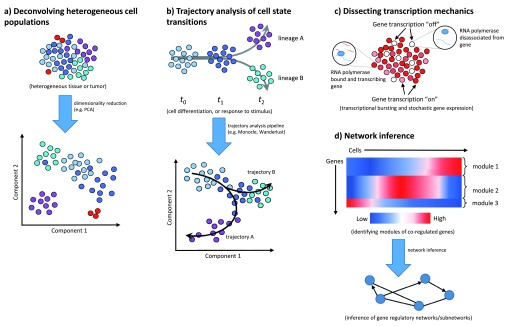
\includegraphics[width=\textwidth]{figures/biological_introduction/sc_purposes.jpg}
         \label{subfig:sc-applications}
         \caption[\textbf{Common applications of single-cell RNA sequencing}]{(a) Deconvolving heterogeneous cell populations. The single-cell resolution level can enhance the identification of rare cell species or subtypes. (b) \textit{Trajectory analysis} of cell state transitions, over the course of dynamic processes such as differentiation or signalling responses to an external stimulus. Recent computational advances, such as Monocle2 \autocite{qiu_etal17} can even reconstitute diverging and lineage-specific trajectories. (c) Dissecting the intricacy of transcription kinetics, inherently stochastic. (d) Network inference. Genes can be clustered by expression profiles to identify modules of co-regulated genes, further unravelled through studying the covariance matricial structure to infer gene regulatory networks. Reproduced from \autocite[Fig .1]{liu_trapnell16}.}
     \end{subfigure}
     \vfill
     \begin{subfigure}[p]{0.4\textwidth}
         \centering
         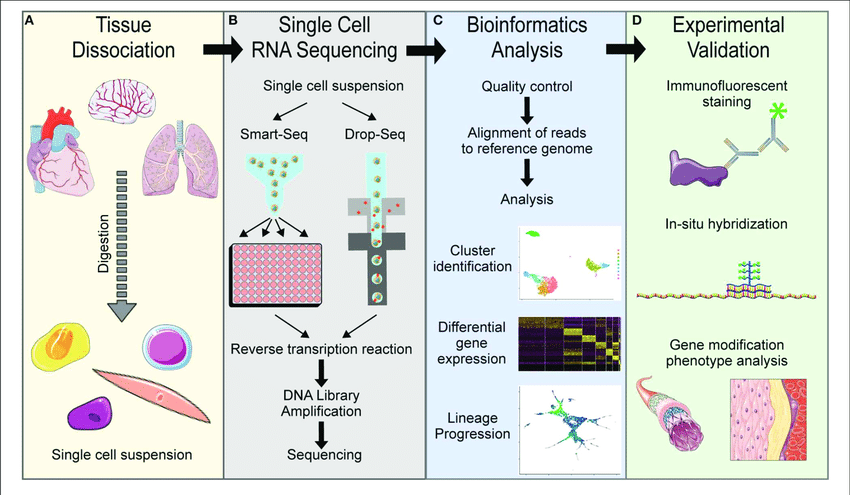
\includegraphics[width=\textwidth]{figures/biological_introduction/sc_pipeline.png}
         \label{subfig:sc-pipeline}
         \caption[\textbf{Overview of a standard single cell RNA sequencing pipeline}]{(A) Tissue dissociation at the cellular level (B) Single cell RNA sequencing of the single cell suspension. (C) Bioinformatics analysis of the library of reads sequenced (see \Cref{subfig:sc-nexflow} for an example pipeline). (D) Experimental validation. Reproduced from \autocite[Fig. 2]{chavkin_hirschi20}.}
     \end{subfigure}
     \hfill
     \begin{subfigure}[p]{0.58\textwidth}
         \centering
         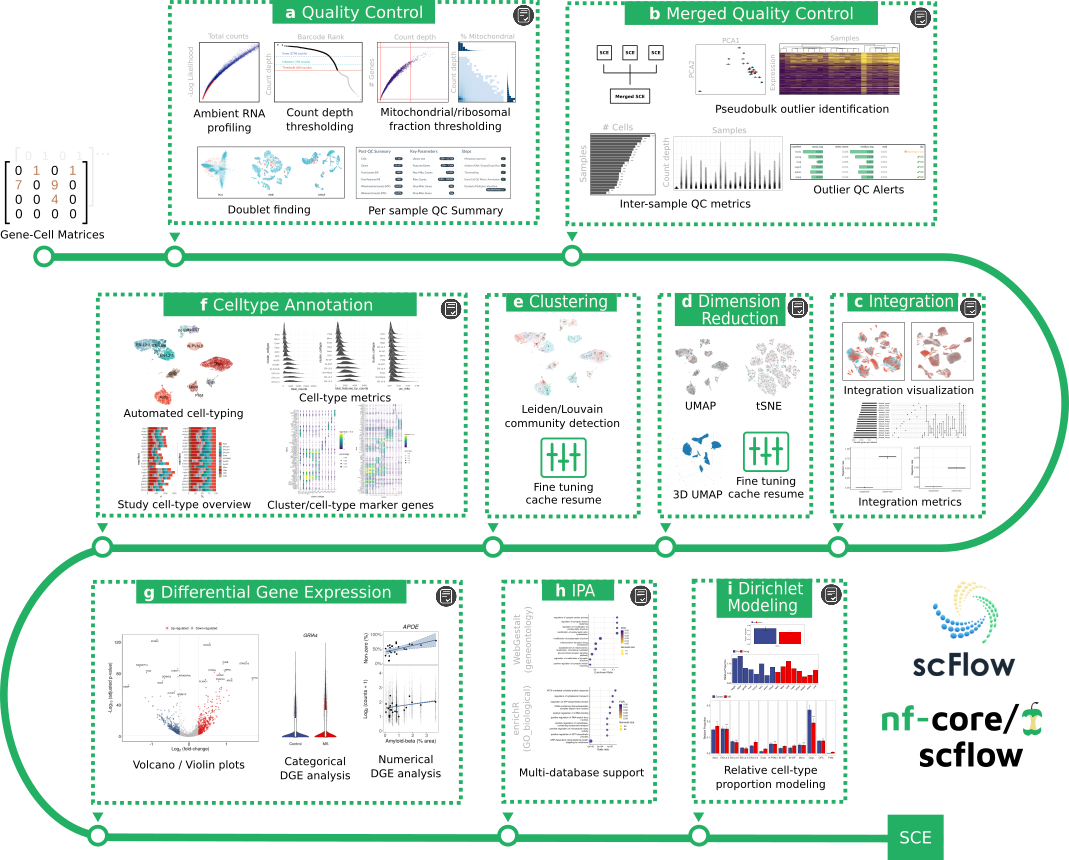
\includegraphics[width=\textwidth]{figures/biological_introduction/sc_computational_workflow.png}
         \label{subfig:sc-nextflow}
         \caption[\texttt{scflow}\textbf{: A Nextflow computational pipeline to analyse scRNA-Seq data}]{(a) Sample quality control including thresholding, doublet identification and removal of dead cells/ empty droplets. (b) Sample outlier identification. (c) and (d) Visualisation of high-dimensional datasets using non-linear dimensionality methods, such as UMAP \autocite{becht_etal19} or tSNE \autocite{maaten_hinton08}. (e) and (f) Louvain clustering \autocite{blondel_etal08} and automated cell-type annotation using marker gene sets. (g) Differential gene expression. (h) Pathway analysis, applying IPA \autocite{kramer_etal14}. (i) Address the inherently compositional nature of cell proportions (unit-simplex constraint) through Dirichlet modelling (see \Cref{sec:perspective-deconvolution} for details) and testing of cell-type composition changes. Reproduced from \autocite{khozoie_etal21}.}    
        \end{subfigure}
\end{figure}

\subsubsection{Spatial transcriptomics}
\label{subsec:st}


While \acrshort{scrna} enables to deconvolve cell populations within a tissue, it does not capture their spatial distribution, nor reveal in real time, \emph{in situ} cellular mechanisms. Indeed, the first step of the  \acrshort{scrna} protocol, namely the library preparation, is a destructive process \autocite{tang22}, which may induce unwanted expression, \enquote{ectopic} (expression not expected to occur in that tissue location), or resulting from the stress induced by the lysis process. This ultimately leads to a suboptimal characterisation and wrongly assignment of cell populations \autocite{vandenbrink_etal17}. 


Precisely, \acrshort{st} methods aim to characterise gene expression profiles while keeping the spatial tissue context. \acrshort{st} encompass two main techniques, each with its strengths and limitations (see also \Cref{subfig:spatial-transcriptomic}): 

\begin{itemize}
  \item \textbf{Image-based approach:} It comprises \emph{in situ} sequencing (ISS, \autocite{yokota_etal20}) and \emph{in situ} hybridisation (ISH, \autocite{vickovic_etal19}), both methods using probes to target specific genes. 
  ISS-based methods increase the amount of transcripts available for sequencing by rolling \emph{amplification} within the tissue after a step of reverse transcription. Each amplified transcript is unequivocally mapped back to its original material and localisation by a padlock probe which encodes an unique ID for each original transcript in each individual cell. Regarding ISH, target sequences are hybridised with a complementary fluorescent probe. 
  While both methods were originally limited in the number of distinguishable transcripts, relying on an unique fluorescent barcode for each transcript, recent developments involving multiplexing with sequential rounds of hybridisation (hence qualified HighPlex RNA imaging (HPRI, \autocite{he_etal22})) and imaging enabled an exponential  computational analysis: with $n$ distinct fluorescent colours and $k$ rounds of re-hybridisation and fluorescence to set apart $k^n$ distinct transcripts.
  
    Both techniques exhibit a strong bias and a lower coverage of the whole genome since they require a prior selection of target genes. Thus, they can not be used to track the apparition of unidentified isoforms or point mutations.  Finally, reads are generally noisier, especially due to the \emph{molecular crowding} phenomena, resulting in spatial overlap of fluorescence signals and restraining the number of fluorescent tags used to a few dozens. However, their single cell resolution (only limited by optical considerations, currently around $\sim \SI{100}{\micro \metre}$) and their better detection and depth per transcript make them better candidates to track temporal dynamics and their influence on the population layout. 
    
    \item \emph{in-situ} capture is a contemporary method that measures the transcriptome level for each of the individual spots of a finely-tuned lattice and tag it with an unique spatial \enquote{ID} barcode, with the spatial coordinates of the associated spot. Then, the sequencing step simultaneously reconstitutes the series of nucleotides composing the original mRNA fragment and map it back to its original spot, a technique consistently termed \emph{spatial barcoding} (see also \Cref{subfig:spatial-barcoding}). One of the current best performing methods, Visium, released by 10x Genomics, displays an increased resolution ($\SI{55}{\micro \metre}$ in diameter) and sensitivity ($\sim \num{10000}$ transcripts per spot) \autocite{nikhilrao_etal20}. 
    Although the sequencing throughput of NGS-based techniques employed in \acrshort{st} is orders of magnitude smaller compared to traditional \acrshort{RNA-Seq} technology, they similarly quantify in an agnostic manner the transcriptome expression, exhibit a higher coverage of the transcriptome compared to the Image-based approach and are cost-saving processes. 
    
    However, the design of the lattice of spots (either a microarray slide or a tangle of beads tethered in well structure, such as HDST \autocite{vickovic_etal19} or Slide-Seq \autocite{rodriques_etal19}), impacting the final \emph{resolution} capture (namely the distance between capture spots), is constrained by physical limitations. Accordingly, it is not rare that the mRNA captured at each spot represents a mixture of cells, rather than an individual entity. In addition, the standardised surface of capture, imposed by manufacturer norms and the computational burdensome of imaging development, may not be adjusted to the biological phenomena or the tissue studied.  
    To mitigate this issue, continuous enhancement of capturing techniques and miniaturisation tends to alleviate these physical and biological considerations, increasing by several factors the spatial resolution and the transcriptomic amplification:  Seq-Scope \autocite{cho_etal21} henceforth sequences at the subcellular resolution, while Pixel-Seq \autocite{fu_etal21} increases by $\sim 200$ folds the depth sequencing while claiming on average a resolution at the single cell size level ($\sim \SI{1}{\micro \metre}$).
    
\end{itemize}

Both techniques return a three-dimensional tensor of transcriptomic expressions, each gene being represented by a matrix of intensities representing its 2D (or even using computational assembling 3D) spatial expression pattern, resulting in the colourised Heatmap pictured in \Cref{subfig:spatial-barcoding}. 


The intricacy of \acrshort{st} is likely to reveal new biological insights, unavailable to standard transcriptomic methods, by adopting an hypothesis-free approach. In ~\autocite[Fig.~2]{rao_etal21}, direct applications from \acrshort{st} are reviewed, adopting a multi-layered view, from the local scale (the cell composition and gene composition of each spot) to the tissue level (detection of \enquote{spatial patterns} or \emph{hotspots}) \footnote{
By capturing in-place, and even in some cases, in-real time, the emph{co-localisation} distribution between hotspots of interacting cell types, \acrshort{st} can infer the intercellular communication patterns.  This approach can be employed, for instance, to strengthen or on the contrary, early discard putative biological interactions between a receptor and its ligand. Computational predictability of interactions arise from literature review, molecular screening, or \acrshort{scrna} correlation analysis (see \Cref{chap:covid19} for a review of physical and computational approaches to predict drug-target interactions notably). Even with robust evidence of physical interaction, if two distinct cell subpopulations are spatially distant and cannot effectively communicate, the possibility of intercellular exchanges is unlikely: indeed, as quantified in \autocite{armingol_etal21}, a significant portion of cellular signalling occurs within the neighbourhood of the releasing cell, operating at the juxtacrine and paracrine levels within a range of \qtyrange{0}{100}{\micro\meter}. This heuristic technique of checking conjectured intercellular communications through co-localisation analysis is visually described in \autocite[Figure 5]{longo_etal21}, and is notably used by SpaOTsc \autocite{cang_nie20}.}. 
Besides, since \acrshort{st} tend to be less destructive compared to other exploratory approaches, preventing structural damage or further cell death, they are intensively used to survey temporal dysregulation patterns of complex, intertwined systems, with applications ranging from neurodegenerative disorders (Alzheimer’s disease \autocite{chen_etal20}, AML \autocite{warnat-herresthal_etal20}) to immuno-inflammatory affections (influenza, \autocite{curras-alonso_etal21}, sepsis, \autocite{janosevic_etal21}). 

\begin{figure}
     \centering
     \begin{subfigure}[p]{0.45\textwidth}
         \centering
         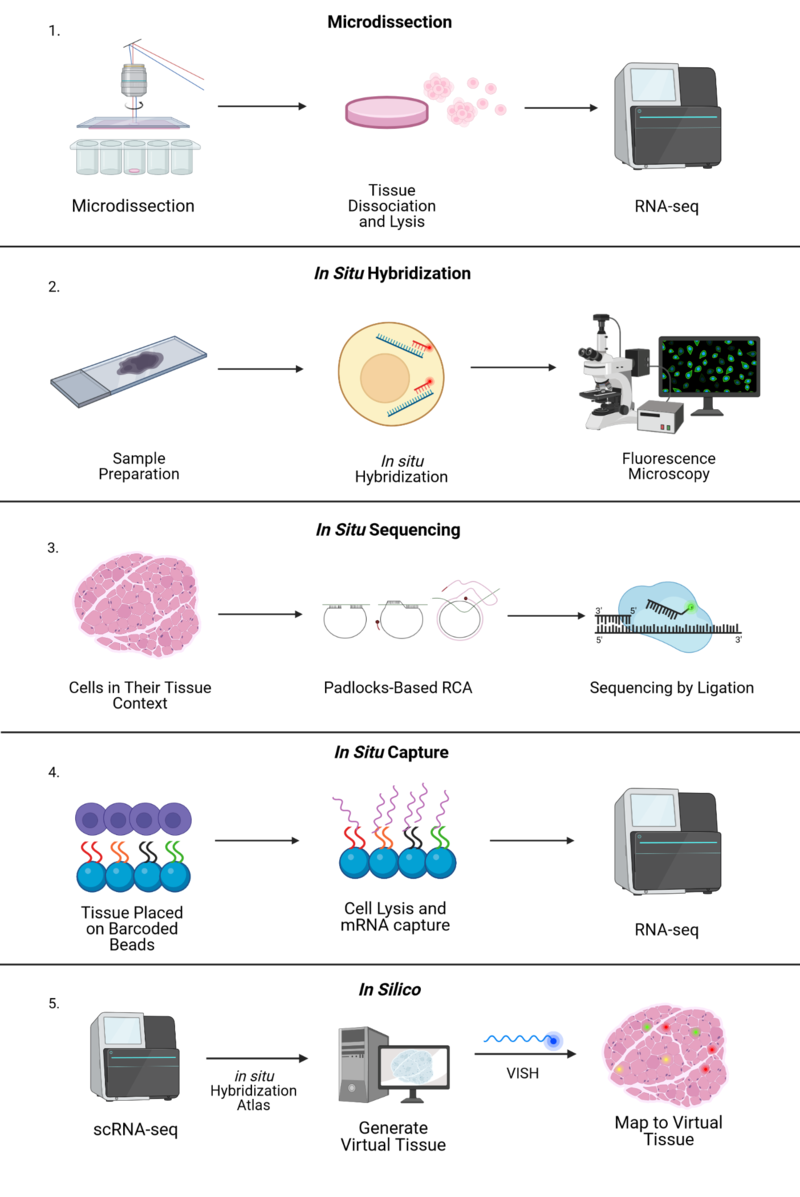
\includegraphics[width=\textwidth]{figures/biological_introduction/Spatial_Transcriptomics_Overview.png}
         \label{subfig:spatial-transcriptomic}
         \caption[\textbf{Overview of Spatial Transcriptomics Methods}]{(1) Microdissection method. (2) \textit{in-situ} Hybridisation method. (3) \textit{in-situ} Sequencing method. (4) \textit{in-situ} Capture method, alternatively named spatial barcoding. (5) \textit{in-silico} method. Reproduced from \autocite[Fig .1]{slifertheryedragon23}, using the BioRender software \autocite{biorender}.}
     \end{subfigure}
     \hfill
     \begin{subfigure}[p]{0.45\textwidth}
         \centering
         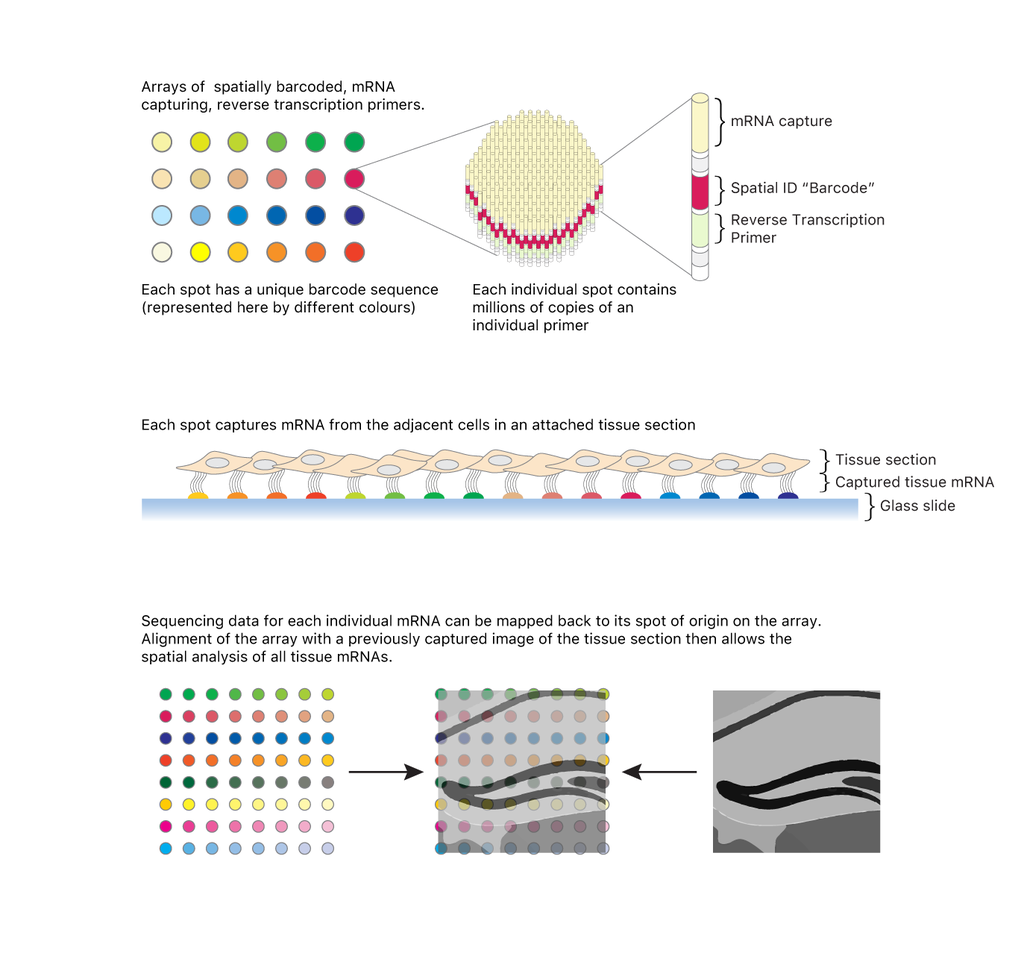
\includegraphics[width=\textwidth]{figures/biological_introduction/Spatial_transcriptomics_detail.png}
         \label{subfig:spatial-barcoding}
         \caption[\textbf{Zoom on the \textit{spatial barcoding} technique}]{Reproduced from \autocite[Fig. 3]{chell23}.}
     \end{subfigure}
     \vfill
     \begin{subfigure}[p]{0.95\textwidth}
         \centering
         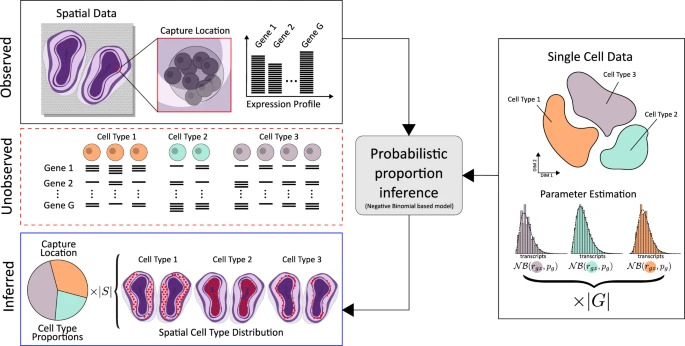
\includegraphics[width=\textwidth]{figures/biological_introduction/sc_deconvolution.jpg}
         \label{subfig:sc-deconvolution}
         \caption[\texttt{stereoscope}\textbf{: A single cell, spatial deconvolution algorithm}]{A deconvolution algorithm is used to model and infer the mixture composition of cell populations at a specific capture site, using annotated single-cell data. Interestingly, the method does not rely on marker genes or gene set enrichment to quantify the cellular composition.  Precisely, the probabilistic model employs a convolution of negative binomial distributions to yield a comprehensive map of the spatial distribution of cell types throughout the entire tissue. Reproduced from \autocite{khozoie_etal21}.}         
         
     \end{subfigure}
\end{figure}

The next bioinformatic milestone in the area is the reconstruction of a real multi-layered model, the only means of unravelling how emerging properties arise from the spatial arrangement and individual cell-cell interactions: promising approaches integrating this aspect are briefly reviewed in my general author's opinion in \Cref{chap:general-perspectives}. 

\subsubsection{The best of both worlds: towards a holistic biomolecular approach}
\label{subsec:sc-and-st}

Nonetheless, the restricted transcriptome \emph{coverage} and \emph{depth} associated with \acrshort{scrna}-\acrshort{st}-based approaches impede their capacity for in-depth exploration, suggesting to bridge both worlds, coupling the versatility of \acrshort{st} investigations with the precision and accuracy offered by \acrshort{RNA-Seq} technologies. An integrative approach is more amenable to unravel the mechanistic processes underlying intricate biological processes, ranging from capturing the temporal dynamics of tissue development through \gls{lineage tracing} \autocite{zhang_etal20} or RNAVelocity \autocite{lamanno_etal18} (\autocite{asp_etal19} applied \acrshort{st} on cardiomyocyte populations at the embryonic stage) to understanding the temporal dynamic involved in the pathogenesis progression (\autocite{maniatis_etal19} identifies a set of 31 co-expression modules temporally correlated with the evolution of amyotrophic lateral sclerosis, coupling spatial barcoding with \acrshort{scrna}). 


There are two primary approaches for integrating \acrshort{scrna} in spatial data: \emph{cellular deconvolution} (see \Cref{sec:perspective-deconvolution} for details) and \emph{mapping}. 

Both methods follow the same workflow subdivided into four stages, often referred to as the four A's (\autocite[Fig. 4]{longo_etal21}):
\begin{itemize}
    \item \textbf{Adopt} From literature, a subset of the tissues or the populations of interest, with intricate spatial patterns, is selected for further analysis. 
    \item \textbf{Assay} Survey the same tissue (to keep the same phenotypical conditions and limit technical variability) with scRNA-sequencing (its higher coverage and unbiased nature makes it a promising candidate for the selection of candidate genes) and spatial barcoding to locate their prevailing location within the tissue. Then, track the spatial and temporal dynamics of this subset of genes with HPRI imaging (recall that this method requires to know in advance the sequence of the genes).
    \item \textbf{Assemble} Using deconvolution and mapping algorithms, generate maps that assigns each coordinate to one cell type. Matching histology images may reveal informative landmarks and help denoising complex areas, such as the tumour leading edge, transition region between cancer and normal tissue. 
    \item \textbf{Analyse} The high-dimensionality of \acrshort{st} datasets was use to corroborate ligand-receptor interactions involved in cellular signalling, or to survey evolving dynamics occurring in a disease progressing condition.
\end{itemize}

\textit{Mapping}, generally employed for high-plex RNA imaging assays, consists first to assign each spatially detected cell to its corresponding (scRNA-seq) profile and secondarily, infer a pattern predicting the location of each scRNA-seq cell based on its transcriptome. Mapping reveals notably useful to determine the general layout of cell populations within a tissue and to identify hotspots or \enquote{niches} (specific and localised microenvironments in which stem cells prevail over fully differentiated cell subtypes). A benchmark of fourteen algorithms that implement mapping through cluster-based approach \autocite{tran_etal20} states that the three best performing were LIGER \autocite{welch_etal19}, Seurat Integration \autocite{stuart_etal19} and Harmony \autocite{korsunsky_etal19}). All three algorithms ultimately retrieve cell types by clustering joined \Gls{st} and scRNA-seq data, which was first projected to a lower-dimensional space. 


Furthermore, instead of surveying only one omic, capturing the simultaneous spatial and temporal evolution of heterogeneous biological data is likely to even increase the exploratory avenues offered by these promising technologies. Hence, \acrshort{scrna} is paired with orthogonal omic information, respectively with epigenomics \autocite{smallwood_etal14}, genomics \autocite{dey_etal15} or proteomics \autocite{amir_etal13}). Another promising avenue aims at integrating within high-resolution tissue images histopathology annotations, such as the cell shape or size. Traditionally, the methods took profit from canonical in-situ hybridisation technics (FISSEQ \autocite{lee_etal14}, TIVA \autocite{lovatt_etal14}) or RNA tomography (Tomo-Seq, \autocite{holler_junker19}).  Another recent alternative is the \emph{stochastic profiling} approach: instead of prospecting at the single cell level and hereby, dealing with small amounts of RNA, this method aggregates the expression of randomly chosen and heterogeneous small pools of cells (around a dozen), increasing the amount of mRNA produced. Then, deconvolution algorithms (\autocite{narayanan_etal16} and  \autocite{andersson_etal20}), are used to computationally dissect the pool of $k$ cells at the individual cell level. To that purpose, \autocite{andersson_etal20} developed a probabilistic framework, named \texttt{stereoscope}, that combines single-cell and $k$-cell data to infer robust and accurate evaluation of the intracellular heterogeneity. Precisely, the distribution of the transcripts are modelled through negative binomial distributions, which are further employed to study the heterogeneous activation patterns from key regulatory genes, as depicted in \Cref{subfig:sc-deconvolution}. 


We refer the interested reader to \autocite{longo_etal21} and \autocite{williams_etal22} for a comprehensive review of spatial transcriptomic and \acrshort{scrna} technologies, with their respective advantages, limitations and computational resources to analyse them.



\subsection{Miscellaneous applications of ngs technologies}
\label{subsec:miscelleanous-innovative-rna-seq}

The versatility of \acrshort{ngs} platforms enable a wide variety of genomic, transcriptomic or epigenomic applications, beyond the mere quantification of known transcripts. In these applications, while the sequencing process is shared across applications, the RNA or DNA library preparation and the bioinformatic algorithms to map and analyse the reads have a strong impact on the accuracy of the downstream analysis performed. 
A brief overview of other applications is described hereafter:

\begin{enumerate}[label=(\roman*)]

\item \textbf{Genomics sequencing:} Three applications benefit from the high-throughput sequencing process of \acrshort{ngs}: WGS (whole genome sequencing), WES (whole exome sequencing) and \emph{de novo} sequencing. Genome-wide association studies(GWAS) are a common approach for identifying disease association patterns across the whole genome: while relying previously on a final set of pre-defined markers interrogated by microarray-based methods, the most comprehensive method of interrogating the 3.2 billion bases of the whole human genome has only emerged with the more scalable and flexible \acrshort{ngs} technology.  In order to decrease the costs, it is also possible to focus only on the set of protein-coding sequences (the exome), since they  gather most of the known disease-causing variants. 

\item \textbf{Transcriptomics} In addition to total mRNA sequencing already discussed comprehensively in \Cref{subsec:RNASeq}, it is also possible to target only transcripts or a specific region of interest to both save costs and get a comprehensive insight on the intricacy of the regulation mechanisms involved, ranging from alternative splicing with isoforms to mRNA mutations or modified enhancer sequences. Notably, targeted resequencing projects has typically a coverage of $500-1000 \times$ against an average of $30\times$ for traditional WGS projects \autocite{li_etal15} \autocite{johansson_etal11}. Such a strategy increases the possibility to detect rare variants, notably somatic mutations in highly-heterogeneous samples (e.g., in the Tumoral MicroEnvironment, with a variety of tumoral clone populations mingled with germline or cells displaying a healthy phenotype).
Finally, it is possible to select upstream microRNAs (short, non-translated nucleotide sequences) that were shown to play a role in the regulation of gene expression (\Cref{subsec:reg-transcript}, \autocite{catalanotto_etal16}, \autocite{moreno-moya_etal14}).

\item \textbf{Epigenomics} Epigenetics aims at understanding the mechanisms underlying the regulation of the transcriptome, deprived from mutations on DNA sequences' causes. This notably includes DNA methylation, smallRNA mediated regulation and PPI interactions with the genome \Cref{sec:gene-regulation}.

\emph{Methylation sequencing} focuses generally on highly regulated regions, such as promoters or heterochromatin, generally enriched in GC sequences, and require specific \acrshort{ngs} technologies able to dive down to the nucleotide level \autocite{zmarzly_etal16}, \autocite{coleman-derr_zilberman12} and \autocite{han_etal07}. The two major methylation methods are Whole-Genome Bisulfite Sequencing(WGBS, \autocite{zhou_etal19a}) and Reduced Representation Bisulfite Sequencing (RRBS, \autocite{sang21} and \autocite{wan_bell20}). 

\emph{protein–DNA interactions} can be precisely surveyed, combining the high-throughput sequencing of \acrshort{ngs} with Chromatin Immuno-Precipitation Sequencing (ChIP-Seq) \autocite{small_etal21}. These methods are used to identify the binding sites for a given protein at the scope of the whole genome. 

\emph{Ribosome profiling} focuses on mRNA strands that migrate to the ribosome complexes, in which they are translated into proteins. Hence, this technique provides a more faithful insight at the protein level compared to classical RNA sequencing (RNA-Seq) \autocite{blevins_etal19}. This information enables an indirect quantification (straightforward to get, compared to direct quantification measures) of the proteome (set of proteins currently translated/produced in the cell), hereby providing an insight on post-transcriptional regulation mechanisms \Cref{subsec:post-transla}, \autocite{kiniry_etal20}, \autocite{yadav_etal21}.   

While some regulation processes occur in localised regions of the genome, other processes modify globally the rate of transcription by acting on the \emph{tridimensional spatial configuration} at the genome scale \Cref{subsec:reg-transcript}. \emph{Chromatin remodelling} is one of the key mechanism involved and is estimated through the combination of \acrshort{ngs} technologies with the ATAC (Assay for Transposase-Accessible Chromatin) technology \autocite{ahmed_ucar17} \autocite{sahu_etal21}.
\end{enumerate}

\section{A glance at the world of immunology}
\label{sec:immunology}
\todo[fancyline]{thèse d'étienne, présentation bio Servier \enquote{Immunology at a glance}, chapter 43 about the immune system}

\paragraph{Overview: the  immune system, the keeper of our body} 
\
The immune system is an intertwined network of cells, organs and molecules that work together to protect the body against infectious agents that may reveal harmful for organism. Such threats are collectively named \emph{pathogens}, ranging from viruses to bacteria and fungi. Its primary role is to early recognise these intruders, in order to eliminate them quickly. The main concept here is to rapidly discriminate foreign molecules as well as self compartments such as tumoral cells that may have a pathogenic effect, from innocuous particles or self sections, for whom no immune reaction is expected. An adjusted \emph{molecular recognition} is a key feature of the immune system, as perturbations of its mechanism is at the origin of the vast majority of immune disorders. 

The immune system is traditionally divided into two interacting schemes: the \emph{innate immune system} and the \emph{adaptive immune system}. 
Ultimately, the immune system plays a crucial role in keeping the homeostasis of the human body, by defending against a wide range of infectious diseases or inner dysregulations. 

\subsection{The innate system}
\label{subsec:innate-system}
The innate immune system is the first line of defence and provides immediate, \emph{non-specific} protection against invading pathogens.  This includes:
\begin{itemize}
    \item \textbf{Barrier defences} Physical barriers, such as the skin and mucous membranes, are the first line of defence, preventing pathogens from accessing the inner environment. However, entire sealing is impossible, since the human organism must interact with its environment, through gas exchange and nutrition to maintain homeostasis and perform vital biochemical functions. Thus, these protections are generally completed with chemical secretions trapping pathogens, specialised organelles such as lysosomes and reservoir of innate cells poised to fend off potential invasion. Finally, the mucous membranes (from mucus, a viscous fluid aimed at trapping viral particles) of the \gls{epithelial} tissues, such as the digestive or airway tract, provide additional barriers to infection. In parallel with the production of mucus, saliva and other enzymes secreted provide a washing action that inhibits colonisation by fungi and bacteria, destroy their cell walls and contribute to the acidity of the medium, killing most of susceptible bacteria.  
    
    \item \textbf{Immune cells} Cellular defence mechanisms rapidly identify proteins that are commonly shared among pathogens by utilizing specialized receptors on their surfaces. Among these, the Toll-like receptors (TLRs) family, for which the Nobel Prize in Physiology was awarded in 2011, holds a prominent place: this class of proteins is remarkably widespread in the animal kingdom, capable of recognising a diverse panel of micro-organisms \autocite{akira_takeda04}. For example, the TLR3 complex binds to double-stranded RNA, a common nuclic organisation in viruses \autocite{matsumoto_seya08} while the TLR4 and TLR5 respectively target the lipopolysaccharide found on the surface of many bacteria \autocite{takeuchi_etal99} and flagellin \autocite{gewirtz_etal01}, the main protein of bacterial flagella. 

    Then, the elimination process differs along with the nature of the cell. \emph{Macrophages} (\enquote{big eaters}) and \emph{neutrophiles} wipe out pathogens that breach the natural physical barriers by \emph{phagocytosis}. Phagocytosis, originating from the Greek term \enquote{cell eater} is the intricate process through which phagocytes internalise and digest foreign intruders and dead cells. After a first recognition stage, the phagocyte encapsulates the intruder in the phagosome, then fuses within its cytoplasm with the lysosome organelle, whose enzymescut into several pieces the foreign molecules. Generally, influx of neutrophils precedes the arrival of monocytes that rapidly differentiate into macrophages within tissues. 
    
    \emph{Natural killer cells} can induce the death of virus-infected cells \footnote{The term \enquote{natural} stems from their direct action, without prior exposure or activation, while the neutralisation mechanism is akin to the TCD8 cell type. Additionally, they are strongly related to lymphocytes involved in adaptive immune response (\ref{subsec:adaptive-system}, making part of a third component}. NK cells proceed by first detecting abnormal surface-receptors proteins, such as stress signals or tumour antigens, and then by releasing toxic molecules that trigger \emph{apoptosis}, a programmed death of the stricken cell. 
    
    More specialised cells involve \emph{dentritic cells}, whose main function is to coordinate the innate and the adaptive response \ref{subsec:collab-innate-adaptive}, \emph{mast cells} contribute to the inflammatory response but are also involved in aberrant reactions such as allergies, along with \emph{eosinophils} and \emph{basophils}, whose original function was the protection against multicellular parasites, such as worms, that usually require an even stronger reaction. 
    
    \item \textbf{Signalling and antimicrobial proteins} While some peptides directly target and induce destruction of pathogens, such as the \emph{complement system}, others dedicate as regulators and coordinators of the immune response. The complement system is a set of of 30 identified proteins in blood plasma that interact with each other in a highly coordinated and sequential manner. This cascade of biochemical reactions leads to the formation of protein complexes that trigger the \emph{lysis} of invading cells (destruction through bursting of the membrane), the opsonisation (marking for destruction) and the recruitment of immune cells to the site of infection. In addition to its role in fighting infections, the complement system also plays a role in other biological processes, such as tissue repair and development.
    
    Interferons interfere with  cells hosting virus, through mechanisms depending on their belonging class: $\alpha$, $\beta$ and $\gamma$. Interferons are released by virus-infected cells and by binding to neighbouring immune cells, they inhibit viral replication or promote the phagocytic ability of macrophages.

    Cytokines can be released by macrophages, dendritic cells, and natural killer cells. While some of them, such as interleukin-1 (IL-1) and tumour necrosis factor alpha (TNF-alpha), promote inflammation by recruiting neutrophils to the site of infection, others, on the contrary, such as interleukin-10 (IL-10) and transforming growth factor beta (TGF-beta) resolve inflammation and promote tissue repair.  
    
    \item The \emph{inflammatory response} (from Latin \emph{inflammare}, \enquote{set on fire}) is the set of events that modify the microenvironment, triggered by an intertwined cellular signalling released upon infection. The first stage often involves mast cells secreting cytokines, such as \emph{histamine}, that promote growth, migration, and activation of endothelial cells, thus contributing to \emph{vasodilation} \autocite{ribatti_etal20}. The dilatation of blood vessels causes the well-known, localised inflammatory response, characterised by the increase of the skin temperature, redness, and enhanced blood flow. Besides, the released cytokines promote the migration of immune cells towards the inflamed region through a process called \emph{chemoattraction} (movement of a cell following the chemical gradient of a signalling molecule). Then, cycles of signalling and response keep on sustaining the inflammation process, with the deployment of the complement system and the continuous recruitment of additional immune cells \autocite{mollaei_etal20}. 

\end{itemize}

For a faster response, it is worth noting that the two main components of the inflammatory response, namely the macrophages and neutrophiles, circulate throughout the body through the lymph system, whereas others reside permanently in organs and tissues, increasing the likelihood to encounter pathogens and a prompt immune response. However, this first line of defence may reveal insufficient to fend off particularly harsh pathogens strengthened by millions of years of co-evolution. Indeed, some pathogens evolve specifically to overbalance the immune defences (a set of mechanisms referred to as \emph{immune escape}), with some bacteria have an outer capsule that prevents recognition, while others are resistant to breakdown within lysosomes. 


\subsection{The adaptive system}
\label{subsec:adaptive-system}
The adaptive immune system, on the other hand, provides a targeted response to pathogens that have already overwhelmed the innate system, through receptors specific to the intruders. Adaptive immunity relies on two types of lymphocytes: B cells and T cells \footnote{Like all blood cells, lymphocytes originate from stem cells in the bone marrow, but while T cells migrate to the thymus, B cells undergo their maturation stage in the bone marrow. Generally, \Gls{hematopoiesis} is the biological process involved in renewing all the cell populations circulating in the blood, while the corresponding scientific field focuses on resolving their lineage relationships.}. 

All receptor proteins on a single B or T cell share the same antigen receptor and recognise the same \emph{antigen}, any foreign molecule detected as non-self and able to elicit recognition (typically, around \num{100000} are present on their surface). To recognise any potential antigen, millions of distinct lymphocytes coexist in the body, each with its own recognition pattern, able to either bind to a protruding antigen surface or circulating agent, such as microbial toxins. 


The adaptive immune response decomposes into four stages:
\begin{enumerate}[label=(\alph*)]
    \item \textbf{cell diversity} This step enables the creation of a large repertoire of unique lymphocytes, which in turn allows for recognising a large pool of antigens, including theoretically even those never encountered \footnote{Studies show that one million of different B cell antigen receptors and 10 million different T cell antigen receptors coexist in the human organism}. Random \emph{alternative splicing} and \emph{gene recombination} are the fundamental somatic processes that facilitate the production of a comprehensive pool of unique sequence arrangements that compose the variable sections of antibodies. This mechanism is commonly known as \enquote{V(D)J recombination} \autocite{bassing_etal02} and is accomplished through a restricted set of genes  \footnote{The individual pieces composing the light chain of the antibodies can be combined in 200 different ways, and even more for the heavy chain, resulting in \num{3.5e6} possible combinations within the B cell repertoire \autocite{guo12}}. Once the original stem cell produces its own rearrangement of the antigen receptors, they remain permanent and are passed on to the daughter cells.
    
    \item \textbf{Self-tolerance} This step aims at eliminating self-reactive lymphocytes, namely those that recognise own molecules as non self, and thus could trigger improper immune reaction against the body's own molecules and cells. These self-reactive lymphocytes are either destroyed through apoptosis, or rendered non functional. 

    \item \textbf{Clonal selection and Cell Proliferation} The activation of the unique set of B or T cells requires the binding between the epitope of an antigen and an antigen receptor, with the match generally occurring in the lymph nodes \autocite[Figure 6, Chapter 43]{campbell_etal20}. But without clonal amplification, no effective adaptive response would be possible. 
    
    Once activated through binding to an antigen, lymphocytes proliferate into a clonal population, whose cells are all identical to the ancestor lymphocyte and bears the same antigen receptors. Then,  they become \emph{effector cells} and mediate a strong and personalised immune response through the action of (1) T CD4 or Th Helper that coordinate the adaptive response, through notably clonal amplification of effective lymphocytes, (2) T CD8 that kill cells infected
by viruses (\emph{host cells}) and (3) activated B cells, the \emph{plasma cells}, that produce soluble proteins called antibodies that circulate freely in the body fluids. The whole process is termed \emph{clonal selection} as only the lymphocytes specific for a particular epitopemultiply. 

Specifically, helper T cells only recognise antigens that are displayed by the class II MHC on the surface of antigen-presenting cells (APC), generally dendritic cells (DC), but it can also be macrophages or B cells. The specificity of the APC-Th Helper connection hinges on the CD4 protein that guarantees a strengthened joint and extensive information exchange between the lymphocyte and the APC. Once activated, TCD 4 secrete cytokines that promote the generation of a clonal population  and trigger two distinct immune responses that depend on the nature of the vector. The several missions and the crucial role of helper T cell as conductor of the adaptive response is summed up in \autocite[Figure 18, Chapter 43]{campbell_etal20}.

The \emph{humoral immune response} involves the release of antibodies by plasma cells, that in turn promote bacteria elimination by facilitating phagocytosis (act as markers of foreign cells) and promoting the complement response. The released antibodies do not directly kill pathogens, but by targeting circulating toxins or epitopes cradled by the class I MHC of infected cells, prevent viral infection or bacterial activity through \emph{\gls{neutralisation}} or \emph{opsonisation} mechanisms. 

The activation of B cells requires a two-factor authentication process: the first contact with a circulating antigen antigen in lymph nodes turns a virgin B cell into a mature B cell and starts clonal amplification. In the mean time, the activated lymphocyte engulfs some foreign molecules by endocytosis and displays them through its MHC class II molecules. Ultimately, it is only when the B cell meets an helper T cell that was activated in parallel by a macrophage or a dentritic cell that it can turn into an efficient Plasma Cell, a true antibody-secreting factory. This two-step activation is clearly described in \autocite[Figure 19, Chapter 43]{campbell_etal20} and in \autocite[Figures 1 and 2, Chapter 21]{dettmer21}. 

In the \emph{cell-mediated immune response}, another subset of T cells, the TCD 8, proliferate and differentiate into cytotoxic T cells. Initiation of the cell-mediated response first requires activation signals from Th Helper, while the identification of the cells to eliminate relies on the detection of an antigen fragment displayed by the class I MHC of infected cells. In a process similar to NK cells \ref{subsec:innate-system}, destruction of host cells involves the release of perforines that puncture the membrane structure (generate \enquote{pores}), leading to cell lysis, and granzymes that cleave essential proteins, leading to cell apoptosis. Cytotoxic T cells are also equipped with an accessory protein, the CD8 marker, that guaranties strong binding all along the destructive process \autocite[Figure 22, Chapter 43]{campbell_etal20}. Even though not directly targeting virus, depriving the pathogens from potential hosts reduces practically the magnitude and the propagation of the infection. 



\item \textbf{Immunological Memory} 
Finally, the immunological memory is responsible for the long-term protection elicited by a prior infection. This protective mechanism differs from the \emph{primary immune response} by a faster and prolonged response (peak intensity within two days against 10 days), with a greater magnitude (the concentration of antibodies or killer T cells increases by two or three folds). 

This heightened secondary response to the same antigen relies on a subset of the effector lymphocytes, called \emph{memory cells}, that were first activated in reaction to an initial exposure of an antigen. While the vast majority of lymphocytes are short-lived and are eliminated once the infection is overcome (notably by an other category of specialised T cells, depicted as \emph{regulatory}), the longer life duration places memory lymphocytes at the forefront to rapidly initiate clonal amplification of thousands of highly-specialised effector cells, in case of second exposure. 

This mechanism is directly leveraged for \emph{immunisation}, namely the artificial introduction of antigens into the body to generate a pool of memory cells. It is also referred to as \emph{vaccination} (from the Latin \enquote{vacca}, \emph{cow}), since the first documented use of the immunisation principle dates back to late 1700's, when Jenner observed that peasants contract the relatively innocuous cowpox disease, they were protected from the damaging outbreaks of smallpox. Nowadays, vaccines are made from killed or weakened pathogens (first generation), inactivated bacterial toxins (second generation, with careful selection of epitopes) or
even genes encoding microbial proteins (third generation, for instance the \enquote{Messenger RNA vaccines} developed by Pfizer or Moderna against the Covid19), all eliciting a first immune response. Vaccination programs enable to dramatically reduce the infant mortality caused by devastating diseases, whose vectors were particularly obnoxious due to their high pathogenocity combined with escape immunity mechanisms. Notably, the smallpox was eradicated in 1980, while polio and measles cases decreased by several folds.

\end{enumerate}


\subsection{Exchange of goodwill between the two immune systems}
\label{subsec:collab-innate-adaptive}

Contrary to the standard approach which opposes the innate system, shared by all animals, to the seemingly more efficient adaptive system, only developed among jawed vertebrates, we show in this point that it is the constant interplay between lymphocytes and other innate cells that together provides this efficient, coordinated and constantly remodelled protection against a variety of pathogens.

The cooperation between innate and adaptive system generates a positive feedback loop whose main stages are reported on \Cref{fig:innate-adaptive-cooperation}, emphasising how much these two systems are closely intertwined:

\begin{figure}
    \centering
    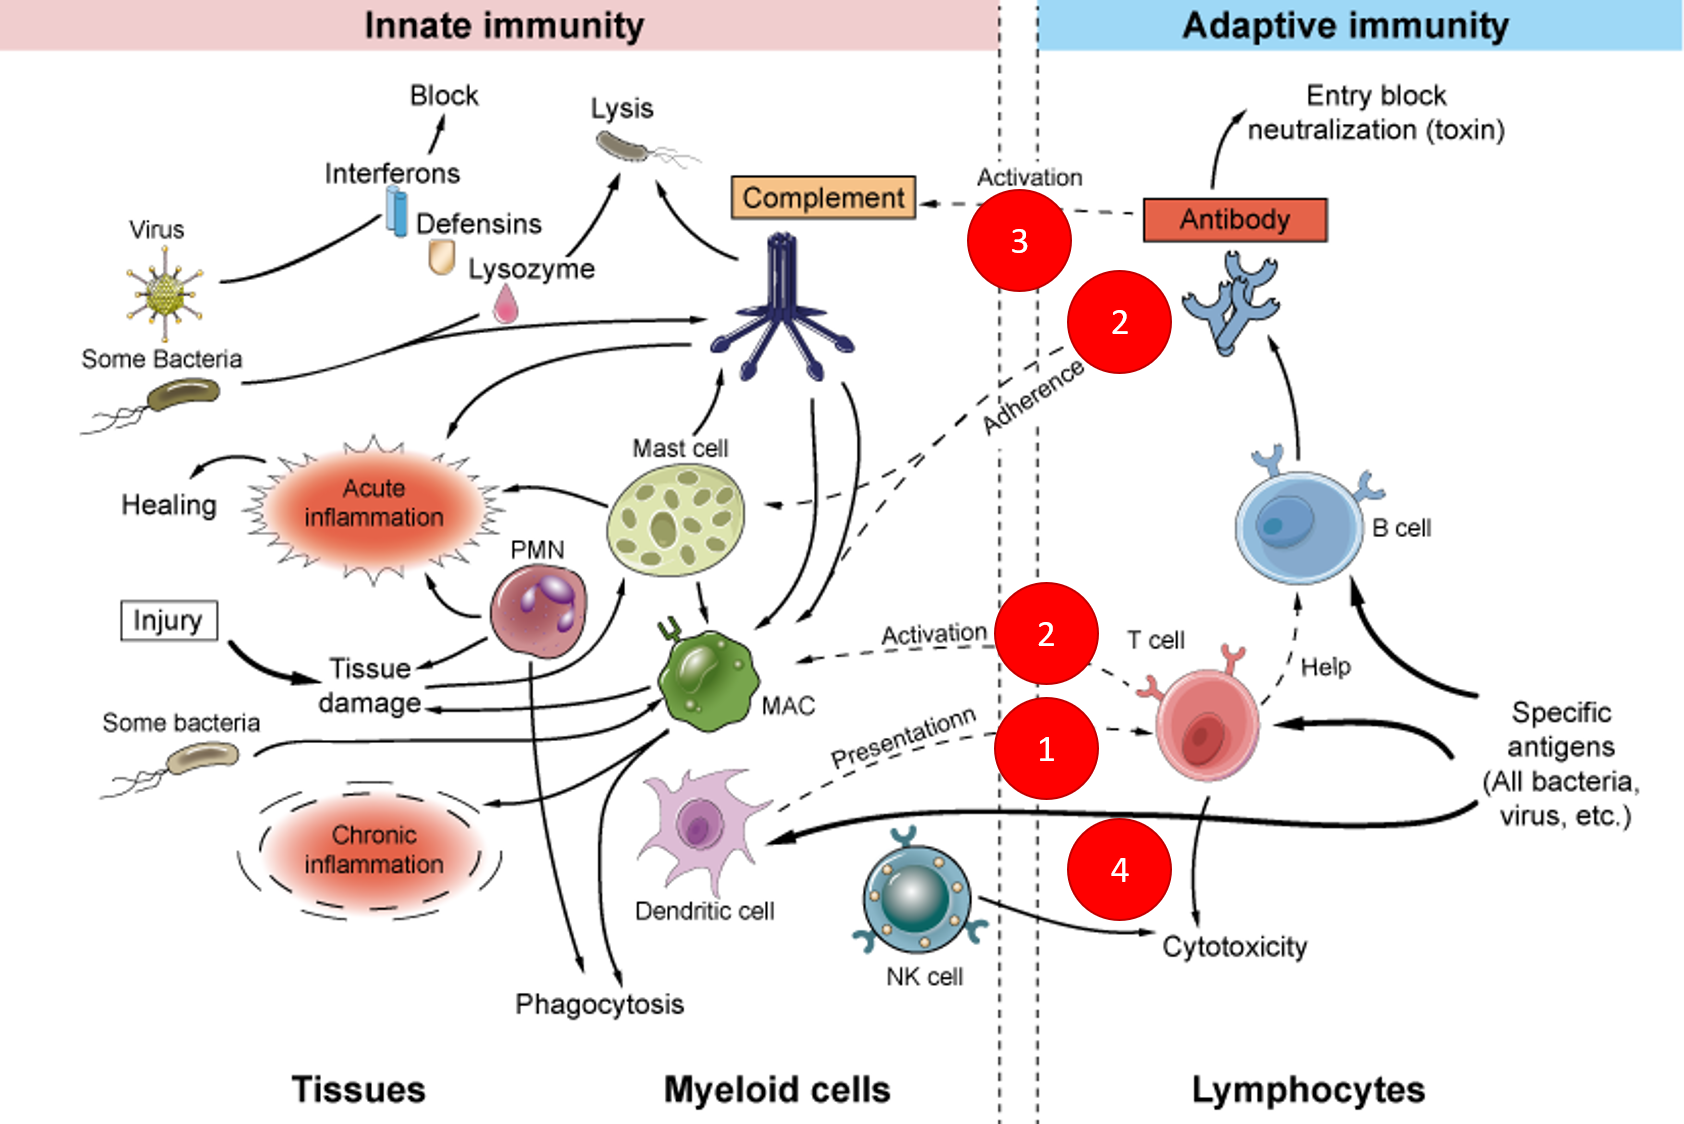
\includegraphics[scale=0.3]{figures/innate-adaptive-cooperation.png}
    \caption[Cooperation mechanisms between the innate and the adaptive immunity]{
    This iconography shows the inner mechanisms intervening in the innate (left) and adaptive (right) response, each able to trigger a cellular (lower half) or humoral reaction (upper half). Reproduced from \autocite[Fig .1]{cdcreativediagnostics20}.}
        \label{fig:innate-adaptive-cooperation}
\end{figure}
    
     However, adaptive mechanisms, although more recent in the evolution, need multiple interactions with the older innate one, reviewed in arbitrary chronological order below:
    \begin{itemize}
        \item A local inflammatory response generally produces \emph{pus}, a mixture of white blood cells, dead pathogens, and debris from damaged tissue, that is flushed away through the lymphatic system towards the lymph nodes, in which permanent macrophages can engulf recognise and display fragment antigens \autocite[Figure 12, Chapter 43]{campbell_etal20}. In the mean time, dendritic cells migrate to the lymph nodes after interacting with pathogens. 
        In both cases, the \emph{phagocytosis} pathway enables to trap antigens, cradled in the MHC II complex, by cleaving the foreign particle into smaller peptides. Finally, the interaction of the MHC with its antigen fragment and the TCR receptor of a TCD4 cell \autocite[Figures 12 and 13, Chapter 43]{campbell_etal20}, triggers an adaptive immune response, through either a cell-mediated or humoral response. A simplified overview of this positive feedback loop is displayed in \autocite[Figures 23, Chapter 43]{campbell_etal20}.
        \item Antibodies directly facilitate phagocytosis, by aggregating toxins or pathogens and marking them to macrophages and neutrophils. In return, the phagocytosis enables macrophages and dendritic cells to capture antigens and ultimately stimulate helper T cells, which activate the very B cells whose antibodies contribute to phagocytosis. Indirectly, cytotoxic T cells, by bursting out cells hosting virus, exposes viral contents and increase the likelihood that APC or antibodies trap foreign peptides, which would have remained out of reach otherwise. 
        \item Complement to neutralisation and opsonisation mechanisms, antibodies interplay with the proteins of the complement system \autocite[Figure 21, Chapter 43]{campbell_etal20}. The associated cascade of biochemical reactions is likely to promote cell lysis.  
        \item The virus uses the cell’s biosynthetic machinery to replicate whom some of them can appear on the cell surface through the MHC class II. Recognition of these protruding epitopes by the complementary antibodies could possibly promote the recruitment of NK cells. Notably, \autocite{gasteiger_rudensky14} premises that T cells could act as antigen-specific sensors to amplify the local immune response of \emph{innate lymphocytes} (alternative name for NK cells, as non specialised cytotoxic T cells).
    \end{itemize}


From the previous subsections, we understand the importance of cross-talks between immune cells in order to provide a balanced immune reaction against any intruder. While it already turned out to be a complex, multi-layered machinery, we have voluntarily hide many parts of its intrinsic complexity, since it would require a whole volume of encyclopaedia and researchers are still debating on the nature or the role of some immune cell types. However, in a desperate process to simplify and sum up the most essential concepts, we represent below the graph of the interactions between the main actors of the immune system, along with the nature of their relationships \Cref{fig:summary-immune-system} 
\begin{figure}
    \centering
    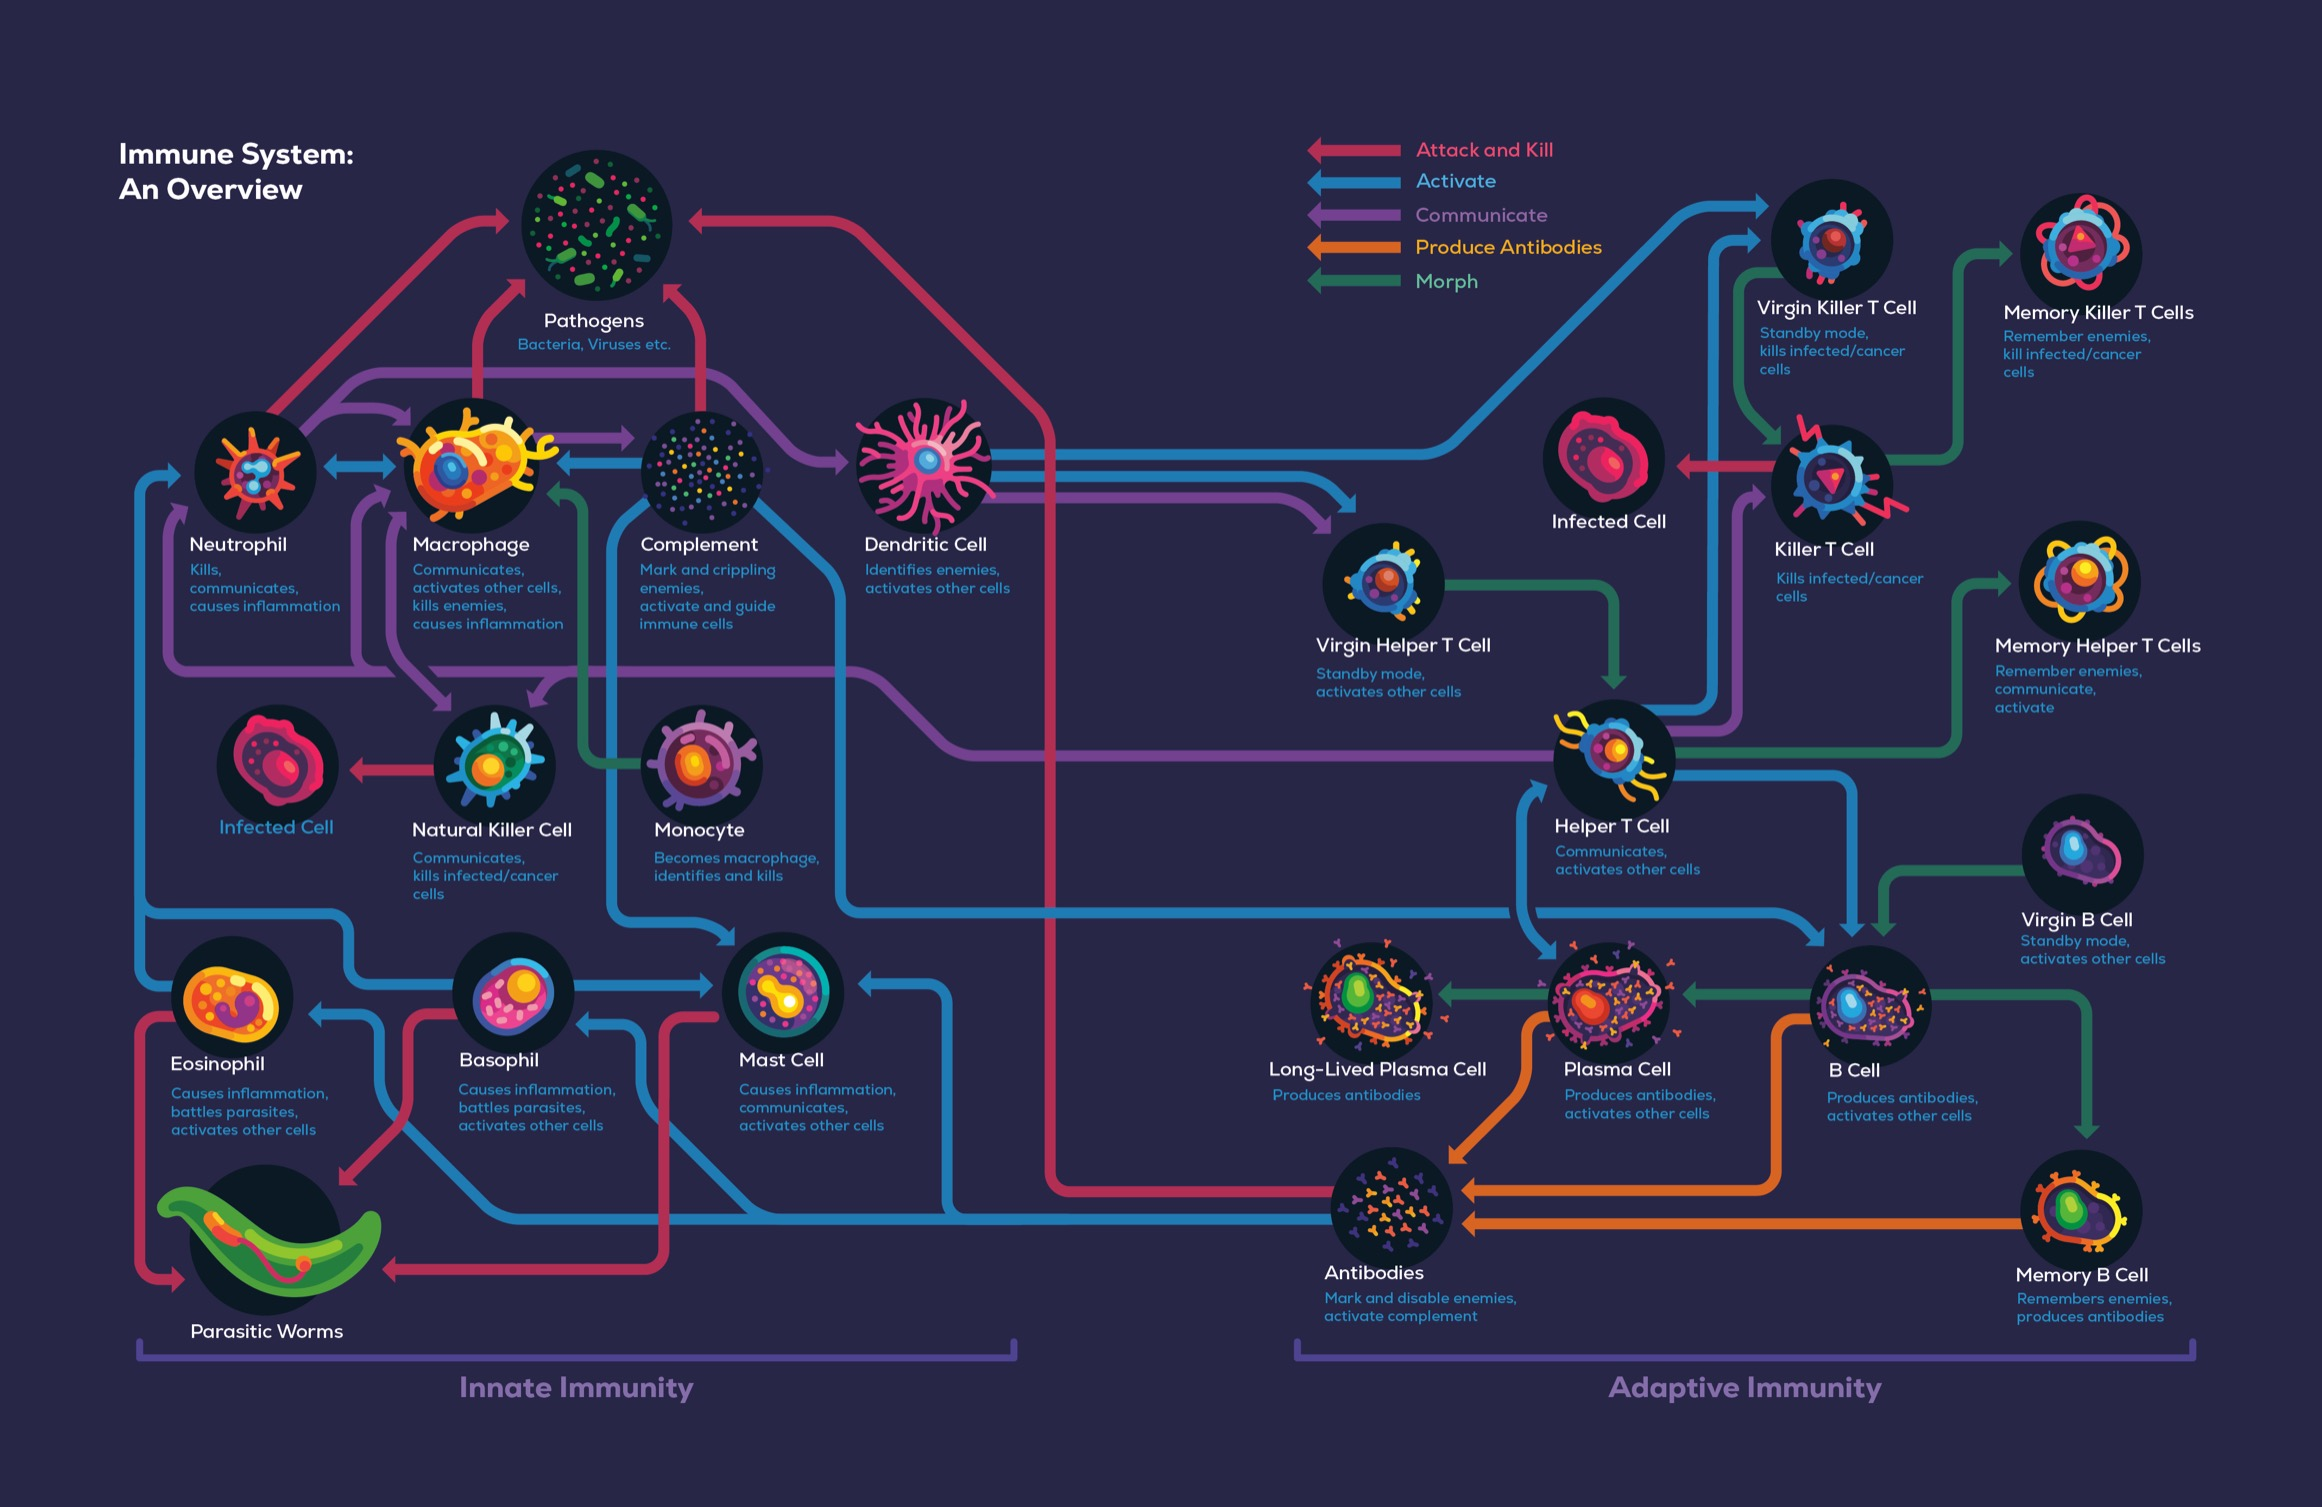
\includegraphics[scale=0.5]{figures/summary-immune-system.jpg}
    \caption[\textbf{An overview of the immune system}]{The red and the blue edges display direct cell-cell interactions, requiring ligand-receptor bound. On the contrary, the purple and orange edges characterise long-range interactions, through the release of respectively chemical signals or antibodies. Finally, the green edge depicts differentiation from one developmental stage to another for a given cell lineage. This figure is reproduced from \autocite[Figure 1, Chapter 42]{dettmer21}}. 
    \label{fig:summary-immune-system}
\end{figure}

In the next section, weinstead talk proficiently about the disorders of the immune system, when it is not anymore in its balanced operating order, and its strong consequences on the human health.

\subsection{Immune dysregulation}

While the immune system is essential to fend off pathogens or wipe out tumoral cells, the strength of the response, especially when occurring at the scale of the organism, results in  detrimental side effects. Hence, a heightened inflammatory response triggered by global tissue damage or blood contamination, is likely to lead to a life-threatening condition, called \emph{septic shock}. It is notably characterised by an increase by several folds of the number of white blood cells, a higher temperature resulting in \emph{fever} at the human organism scale and low blood pressure. We discuss of one of these exacerbated mechanisms in the context of \enquote{cytokine storms}, life-threatening events that occur among many patients overwhelmed by the Covid19 infection, in \Cref{sec:covid19-repurposing}. 

Additionally, not only pathogens can be recognised as non-self, but also any foreign molecule, even issued from other human bodies. The huge number of variations of the  MHC molecules \footnote{the MHC complex not only displays antigen fragments, but a subset of the proteins composing it, the Human leukocyte antigens (HLA) act as an identity card that asserts the immune system that the investigated cell belongs to self} between two individuals prompts transplants or grafts rejection. The only way to counterbalance rejection is to pair match the MHC molecules of the donor and the receptor as much as possible, and to use immuno-suppressor drugs.

A similar mechanism is involved in blood transfusions, but instead of the HLA complex, glycoproteins on the surface of red blood cells are recognised as foreign, eliciting lysis of the transferred blood cells, necrosia and kidney failure. For long, the only way to overcome this process was to control, prior to the transfusion, that the the patient and the donor had compatible blood groups (based on one of the two possible glycoproteins, A or B,  or absence of both of them, marked as O, knowing that patients could only receive blood cells with antigens already present in their organism).
\autocite{olsson_clausen08} reviews pioneering studies made in the development of enzymatic conversion of blood group A and B red blood cells to O for creating a universal blood supply. This includes the use of novel bacterial exoglycosidases with improved properties for cleaving A and B carbohydrates.


Nonetheless, all previous situations correspond to an expected behaviour of the immune system against foreigners, and it is either medicine progress or particularly virulent pathogens that trigger life-threatening conditions. However, the immune system can display aberrant behaviour, often elicited by a failure of the regulation mechanisms (see \Cref{subfig:immuno-vs-cancer} and \autocite{schnell_etal20}). Bad regulation of the immune system often come as the two sides of a coin: \emph{dysregulation} of the immune system leads to an over-activation of the immune system \autocite{rosenblum_etal15}, while \emph{misregulation}, an under-activation of the immune system plays a prominent role in the evolution of the cancer, acting as the prime actor of immune escape \autocite{chakraborty_etal22}. Although auto-inflammatory diseases are typically not fatal by themselves, they can severely compromise the health and well-being of afflicted patients. The Sjögren's syndrome, a condition upon which my attention was particularly focused  is studied in further details in \Cref{sec:sjogren-clustering}. Briefly, we display on \Cref{subfig:autoimmune-origin} below a possible causal factor that elicits the production of self-antigens, and the state-of-the-art parthenogenesis of one of the most common inflammatory ailment in \Cref{subfig:cross-reactivity}, namely sclerosis, best known for taking the life of Stephen Hawking.


\begin{figure}
     \centering
     \begin{subfigure}[p]{0.45\textwidth}
         \centering
         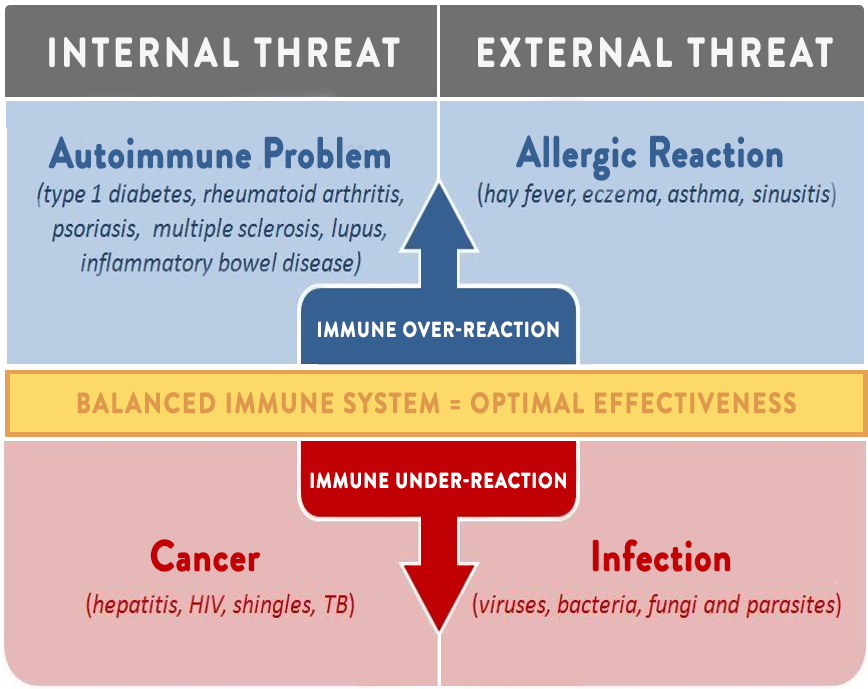
\includegraphics[width=\textwidth]{figures/immuno/The-Link-Between-Cancer-and-Autoimmune-Disease.jpg}
         \label{subfig:immuno-vs-cancer}
         \caption[\textbf{Autoimmune diseases and cancers: the two sides of the same coin.}]{Cancer and autoimmune diseases represent two distinct pathological states. Regarding cancer, the main mechanism involving immune cells is \textit{tumour escape}, in which the immune response is incapable of eliminating self-cells that have undergone transformation. Conversely, autoimmune diseases are characterised by an overactive immune response directed towards self-particles wrongly recognised as antigens, resulting in tissue damage and chronic inflammation. However, autoimmunity and cancer both hinge on a failure of the immune system in controlling abnormal cell proliferation (respectively auto-reactive immune cells or tumour cells). Furthermore, both ailments share analogous mechanistic immune responses, including the recruitment of phagocytes and neutrophils, as well as the activation of hypoxia and angiogenesis processes. Reproduced from \autocite[Fig .4]{sarah18}.}
     \end{subfigure}
     \hfill
     \begin{subfigure}[p]{0.45\textwidth}
         \centering
         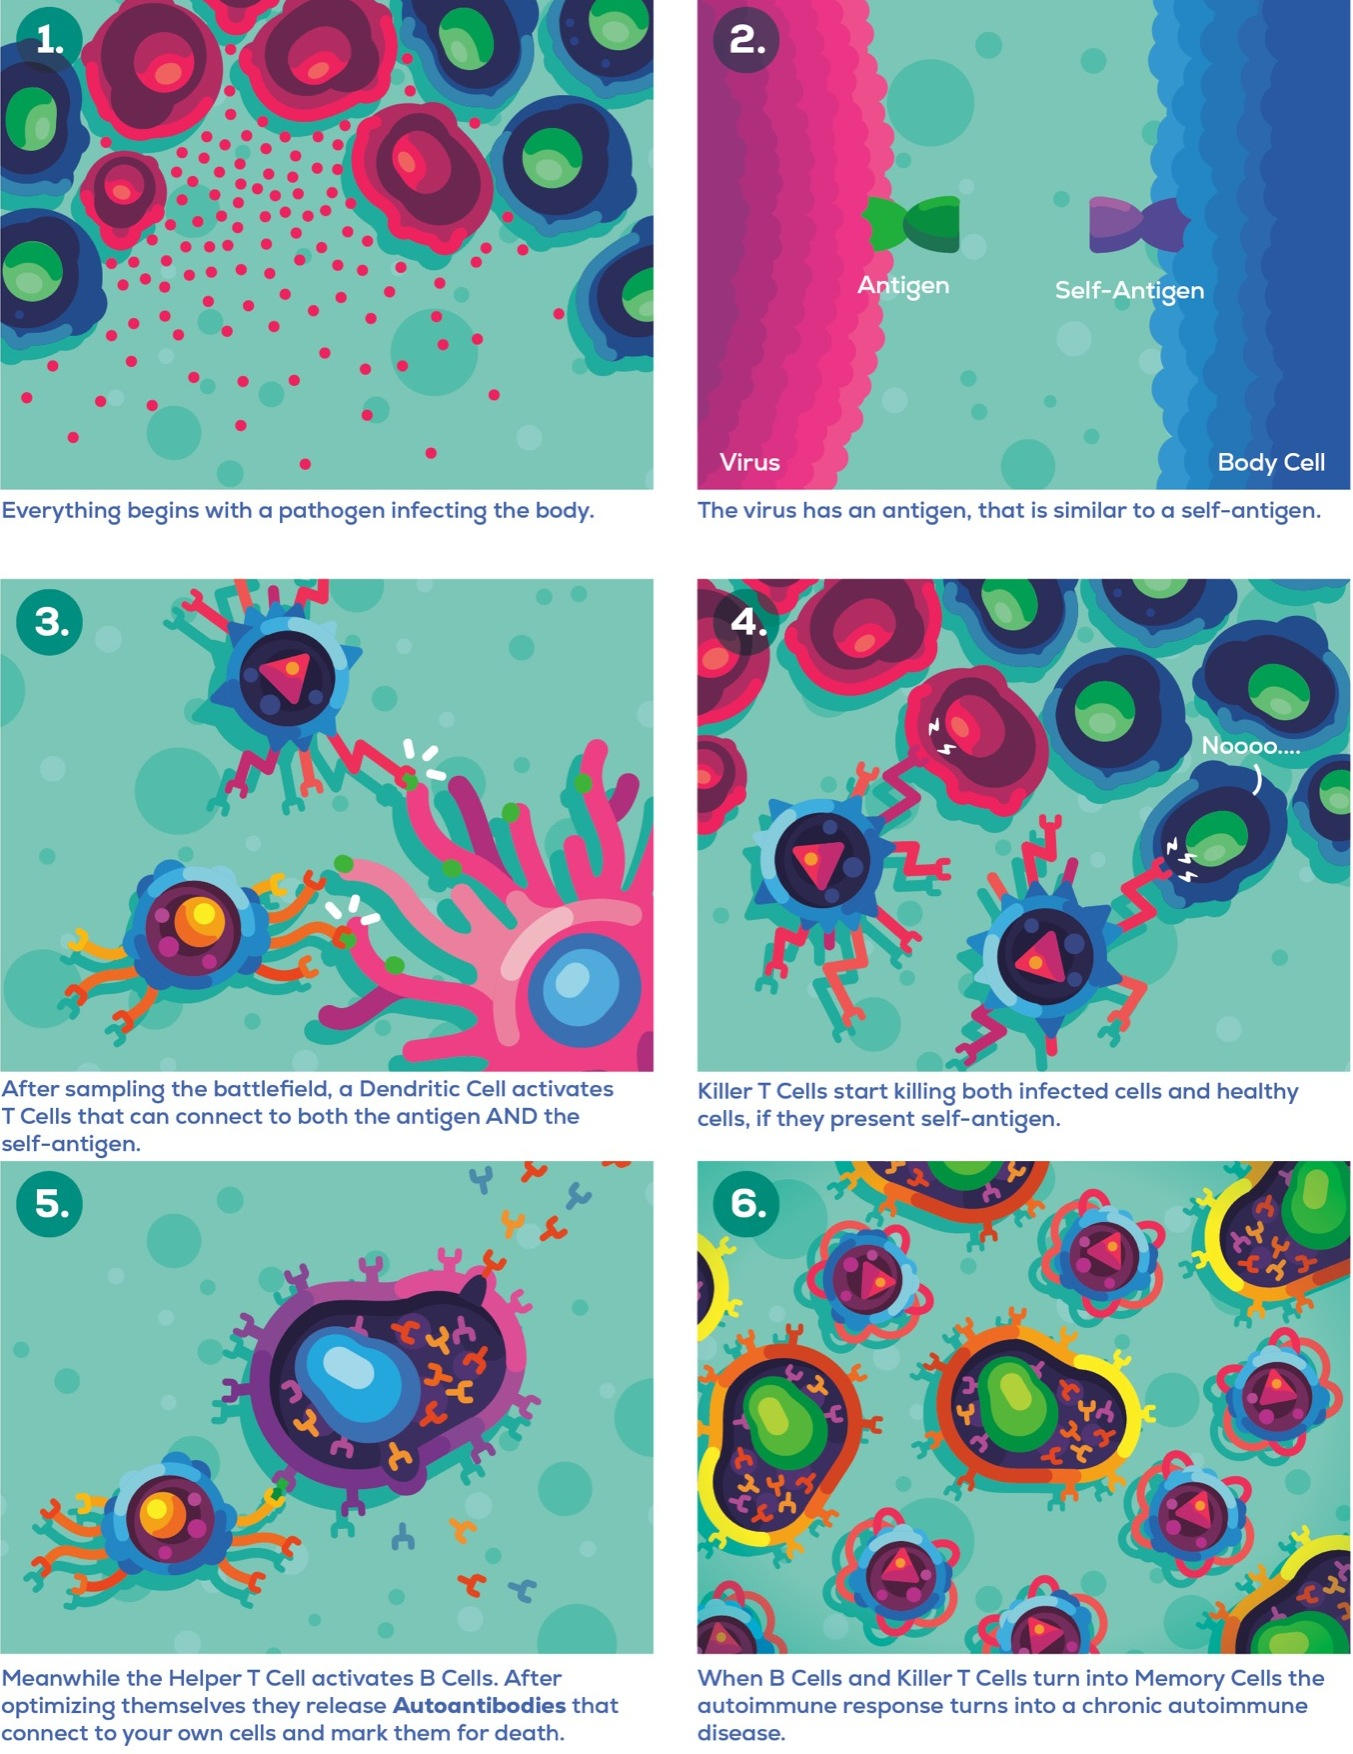
\includegraphics[width=\textwidth]{figures/immuno/kurzgesagt_autoimmune_origin.jpg}
         \label{subfig:autoimmune-origin}
         \caption[\textbf{Cross-reactivity, a prominent etiological factor in the initiation of autoimmune diseases.}]{Dysregulation at several layers of the immune system,  such as the complement system, interferon or cytokine production, can contribute to a variety of diseases, including autoimmune diseases (Crohn’s disease), inflammatory disorders, and infections, notably when the antigens hide from the immune system or when own molecules are recognised as non-self. One major etiological factor which may elicit the genesis of auto-immune diseases is the close proximity of the epitopes present in ubiquitous bacteria with fragments of endogenous molecules. Reproduced from \autocite[Fig. 1, Chap. 40]{dettmer21}.}
     \end{subfigure}
     \vfill
     \begin{subfigure}[p]{0.8\textwidth}
         \centering
         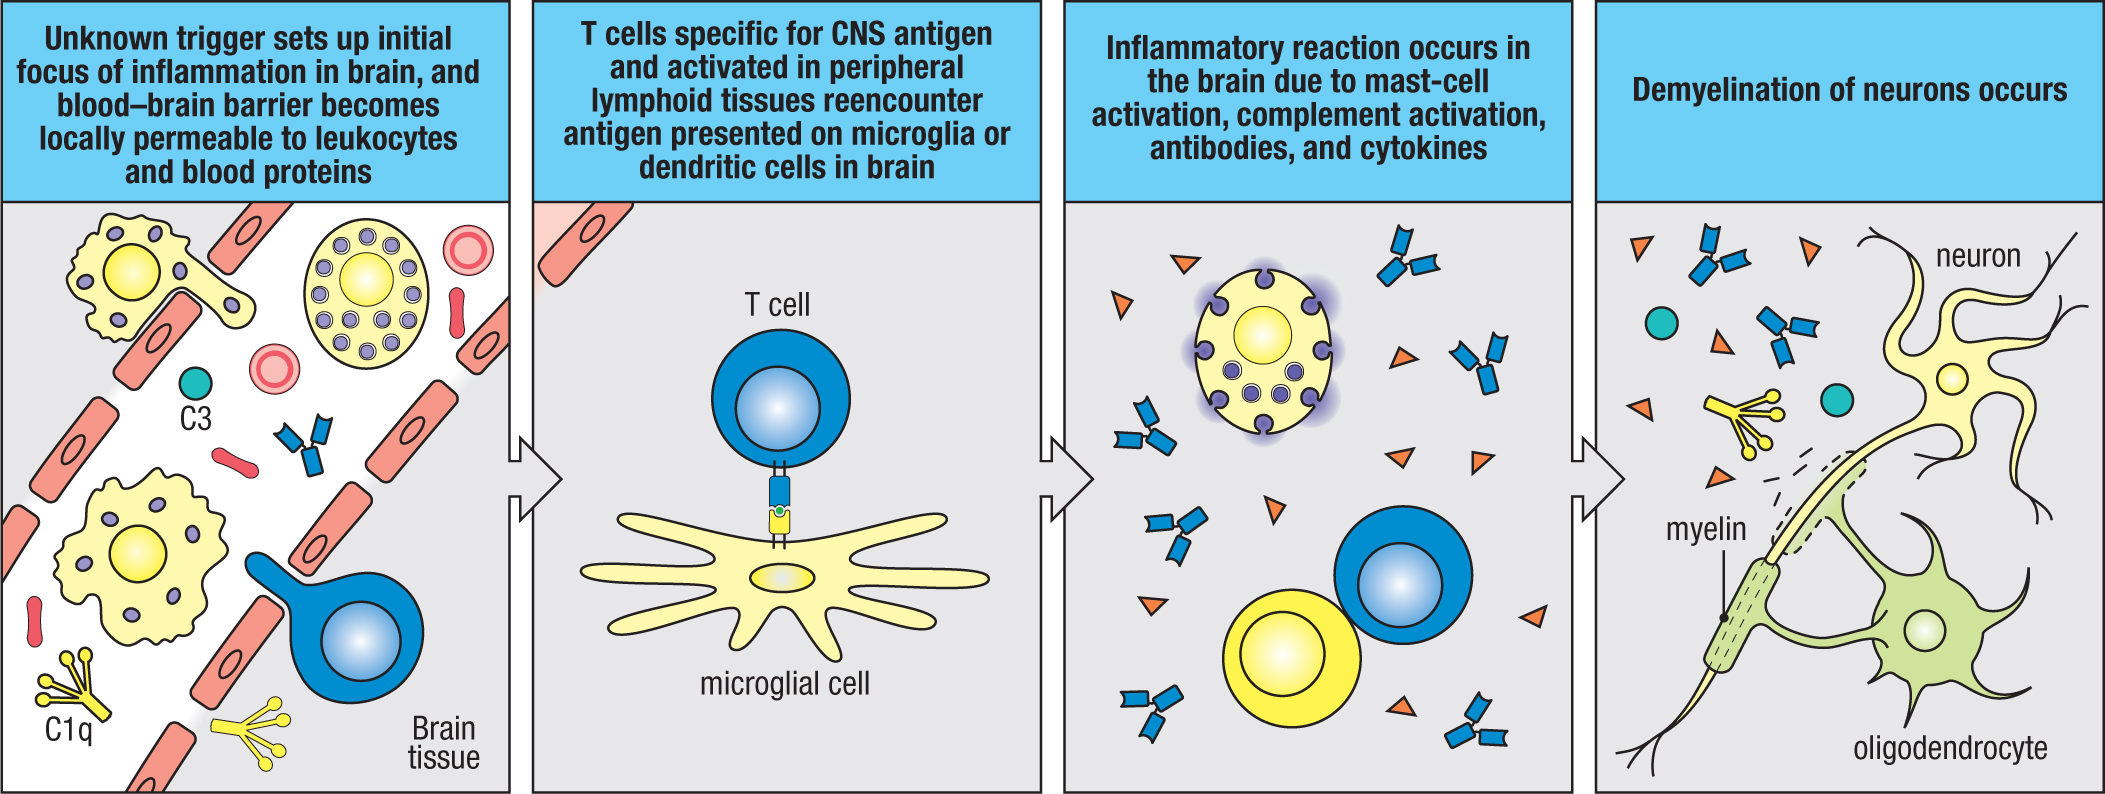
\includegraphics[width=\textwidth]{figures/immuno/cross_reactivity.jpg}
         \label{subfig:cross-reactivity}
         \caption[\textbf{The pathogenesis of multiple sclerosis (MS).}]{MS disease is among the affections studied in the Preciseads cohort \autocite{soret_etal21} \autocite{barturen_etal21}, a large European initiative aimed at deciphering the mechanisms involved in five systemic autoimmune diseases. It is also one of the three inflammatory illnesses, commensurate with those tailored for Sjögren's disease and Systemic Lupus Erythematosus (SLE). The objective is to release within five years promising groundbreaking treatments (see \Cref{sec:sjogren-clustering} for details). While the precise etiology of MS remains elusive, however, the immune mechanics involved afterwards are relatively clear. In inflamed regions, autoreactive T cells  infiltrate the brain through the blood-brain barrier and target brain antigens displayed on microglial cells. Upon contact, they secrete cytokines including, but not limited to IFN-$\gamma$, which in turn further enhance inflammation by chemio-attracting additional cells and complement proteins. Reproduced from \autocite[Fig. 15.25, Chap. 25]{murphy_etal22}.}
     \end{subfigure}
\end{figure}


In conclusion, it is important to recall from the previous section that the immune system is an intricate and interconnected network of cell populations and cytokines interplaying altogether to safeguard the body against foreign invaders. However, even a slight disruption in one of these mechanisms can result in a potentially life-threatening condition. For example, an overstimulation of T and B cells can lead to the development of an autoimmune disease, wherein the body begins to attack its own cells. On the other hand, an over-activation of the regulatory system can result in chronic infections, similar to those observed in patients with AIDS, or the unabated proliferation of malignant tumours.
	Related with auto-immune subjects, and having personally to debate with my acknowledges on the hypothetical benefits of alternative therapies over complex, costly treatments designed by pharmaceutical companies, you should never fall for the miracle effects claimed by the supplement industry, above all from the homeotherapy branch. To quote the author of the \texttt{Kurzgesagt – In a Nutshell initiative}, \autocite{dettmer21}: 
	\begin{displayquote}
	At least for now, there are no scientifically proven ways to directly boost your immune system with any products that are easily available. And if there were, it would be very dangerous to use them without medical supervision.
	\end{displayquote}
	 Indeed, the assertion of enhancing the immune system is predicated on the notion that a balanced immune system is preferable to a robust but unguided one. In reality, the process of recalibrating the crosstalk between the components of the immune system to restore homoeostasis is challenging, highly specific to the disease, and impervious to any panacea or cure-all substance.
	



%\subsubsection{Auto-immune diseases}
%\label{subsec:auto-immune disease}



%\subsubsection{Immunology-oncology}
%\paragraph{Overview: the hallmarks of cancer}
%\paragraph{Pro and anti-tumoral environments}
%\todo[fancyline]{The tumoral micro environment, the text below refers methods from \autocite{longo_etal21}}
%Although spatial transcriptomics analyses of several disease microenvironments exist, tumour microenvironments are presently the most extensively studied46. Tumour microenvironments are particularly heterogeneous and have complex, spatially restricted interactions with the immune system47,48. Until recently, the ability to interrogate the inner workings and heterogeneity of the tumour microenvironment has relied largely on bulk RNA-seq49. scRNA-seq has advanced our understanding by identifying cancer subpopulations that can drive drug resistance, predict metastatic risk and provide prognostic value50,51.
%A recent study combined spatial barcoding and scRNA-seq to localize an immunosuppressive tumour-specific keratinocyte subpopulation to a fibrovascular niche at the tumour borders (as defined by aligning haematoxylin and eosin images) in human squamous cell carcinoma33. This population expressed genes associated with immunotherapy resistance and numerous ligands inferred to modulate cancer-associated fibroblasts, suggesting ways tumour subpopulations may promote local immunosuppression. In pancreatic ductal adenocarcinoma, another study intersected scRNA-seq and spatial barcoding with annotated haematoxylin and eosin images to reveal that inflammatory fibroblasts play a significant role in cancer stress responses34. In addition to providing insights into tumour resistance and stress responses, such integrated data may offer insight into clinical prognosis. For example, one study observed that greater heterogeneity of a transition area within cross-sections of melanoma metastases was associated with poorer patient survival35. Furthermore, spatial data enabled the identification of the most abundantly expressed genes in the transition area
%\todo{Hétérogénéité tumorale et plasticité dans l’espace et le temps, conférence (et aussi pour le TME)}
%
%\paragraph{Monoclonal treatments}
%
%However, cultivated monoclonal antibodies are issued
%from the same ancestral B cell and amplified through multiple division cycles. Monoclonal
%antibodies are also being used as therapies
%for a growing number of human diseases,
%including many cancers.
%
%














 \leadchapter{Three main distinct factors contribute to the variability of the transcriptomic expression between samples (\Cref{fig:variability}): the environmental condition of the sample (disease state, tissue location, \ldots), the genotypical condition (\acrshort{snp}, haplotypes, \ldots) and the cellular composition. 
In addition, part of this variability proceeds from technical factors, while defining and identiying cell populations,  even at the single cell level, can be challenging: indeed, additional heterogeneity in gene expression may result from the existence of multiple, undescribed subpopulations, from different developmental stages or from asynchronous biological processes (e.g, the cell cycle or the circadian rhythm), and the inherent stochasticity of the transcriptome regulation kinetics \autocite{buettner_etal15}.

\begin{figure}
\centering
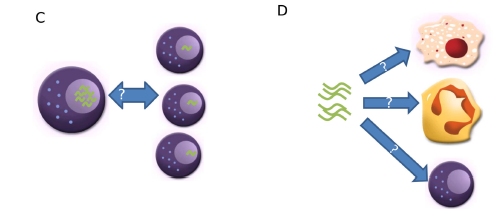
\includegraphics[width=0.7\textwidth]{figures/deconvolution_roles.PNG}
\caption{Sources of heterogeneity in biological samples.}
\label{fig:variability}
\end{figure}

In that context, numerical cellular deconvolution methods, by inferring automatically the composition of complex and highly-heterogeneous biological systems, are promising tools in the quest of the identification of causal drivers and understanding intricate biological mechanisms. 
}


\chapter{Cellular deconvolution}
\label{chap:deconvolution-state-of-the-art}

\section{Deconvolution objectives and main challenges}
\label{sec:deconvolution-challenge}

Over the years, the analysis of the transcriptome has substantially
contributed to our understanding of the processes involved in human
development and disease, but the complex nature of samples and tissues
under investigation has been largely neglected. Indeed, the mean
expression level of a gene differs between different cell subsets, while
in classic bulk transcriptomic analysis, only transcriptomic expression
averaged to the tissue level are provided. Finally, technical artefact
may confound the biological signal.

Additionally, the cell subset proportions themselves show high
variability between individuals, or even within a given tissue, driven
by physiological and pathological processes that induce \emph{cell
motility} and \emph{cell differentiation} (e.g infiltration and
differentiation of the monocytes into macrophages in reaction to a
tissue infection) \autocite{shen-orr_gaujoux13}. Therefore, observed changes in gene expression might
be the result of underlying differences in cell type proportions between
samples, biological differences due to clinical condition or a
combination of both \autocite{kuhn_etal12}.

One of the most common statistical analysis to identify key drivers of a
change in the biological condition is DGEA (differential gene expression
analysis), where in the most common case, we test whether the difference
of the mean expression of a given gene between two biological conditions
(often control versus disease) is statistically significant, with the
\emph{limma} R package being one of the most used
\autocite{smyth_etal22}. Analyses not accounting cell type composition as a confounding factor in
DGEA present suffer from three main drawbacks:

\begin{itemize}

\item
  If a cell population's proportion is correlated with the phenotype of
  interest, cell-subset agnostic DGEAs lose in \emph{specificity}, as
  they are prone to identify false positive differentially expressed
  genes. Ideally, differences due to biological condition should be
  decoupled from those resulting from a change of composition of the
  heterogeneous mixture.
  
\item On the other hand, differences in genes expression expressed by minor cell subsets may be masked by the high variation of the cell population
composition between samples or by the expression of the same gene in a
dominant cell type. This induces a dilution of the signal and a loss of
specificity. Indeed, in \autocite{whitney_etal03}, most of the inter-variability of gene expression within healthy patients was brought by a variation in the neutrophils
population, a largely dominant cell population in most biological
samples composing up to 70 \% of the total cell composition. 

\item As a consequence, not accounting for the cell composition makes it harder to determine the main causal driver of the biological dysfunction observed, especially the cell subset responsible for the observed signal, as illustrated schematically in \Cref{fig:deconvolution-confusing-variable}.
\end{itemize}

\begin{figure}
\centering
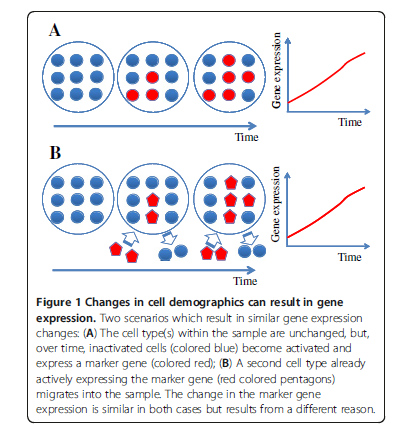
\includegraphics[width=0.7\columnwidth]{figures/dgea_cytometry_consequence.PNG}
\caption{Illustration, from an \autocite{shoemaker_etal12} example, of how two completely distinct causal drivers, result finally into the same global transcriptomic profile.}
\label{fig:deconvolution-confusing-variable}
\end{figure}


 





As suggested by \autocite{baker16}, along
with platform specific frameworks, incorrect data processing or other
technical batch effects, native heterogeneity of transcriptomics data
may explain the lack of reproducibility met currently . Indeed, several
studies have shown that the sensitivity and specificity of DGEAs
increases by integrating the cell population factor obtained from the
deconvolution of bulk expression Shen-Orr et al.
\autocite{shen-orr_etal10}. This is especially true
for highly heterogeneous tissues, such as peripheral blood composed of
many different immune cell subsets or tumoral tissues, with presence of
both normal and malignant cell types of possibly several stems.

Accordingly, the analysis of the interaction between the cell
proportions and the corresponding transcriptomic activity can help in
providing new insights in complex diseases, such as improving the
prognostic of a complex disease (probability of evolution to a more
severe form or to remission\ldots). For instance, an increase in the
proportions of oxyphil cells in the parathyroid gland is correlated to
the severity of the chronic kidney disease
\autocite{ding_etal20}. A reduced
proportion of neuronal cells in Alzheimer's patients increases the risk
of dementia \autocite{andrade-moraes_etal13}. On the other hand, computational methodologies, by decoupling
the sources of variability in heterogeneous data, can help in preventing
wrong associations between specific molecular marker (genes in
transcriptome-wide association studies (TWAS) or methylation CpG sites
in Epigenome-wide association study (EWAS)) to a phenotype of interest.
For example, some genes were down regulated in severe states of the
Alzheimer's disease in relation with a decrease in the number of neurons
expressing them and and not because of a causal biological mechanism
\autocite{mathys_etal19}.

%\begin{figure}
%\centering
%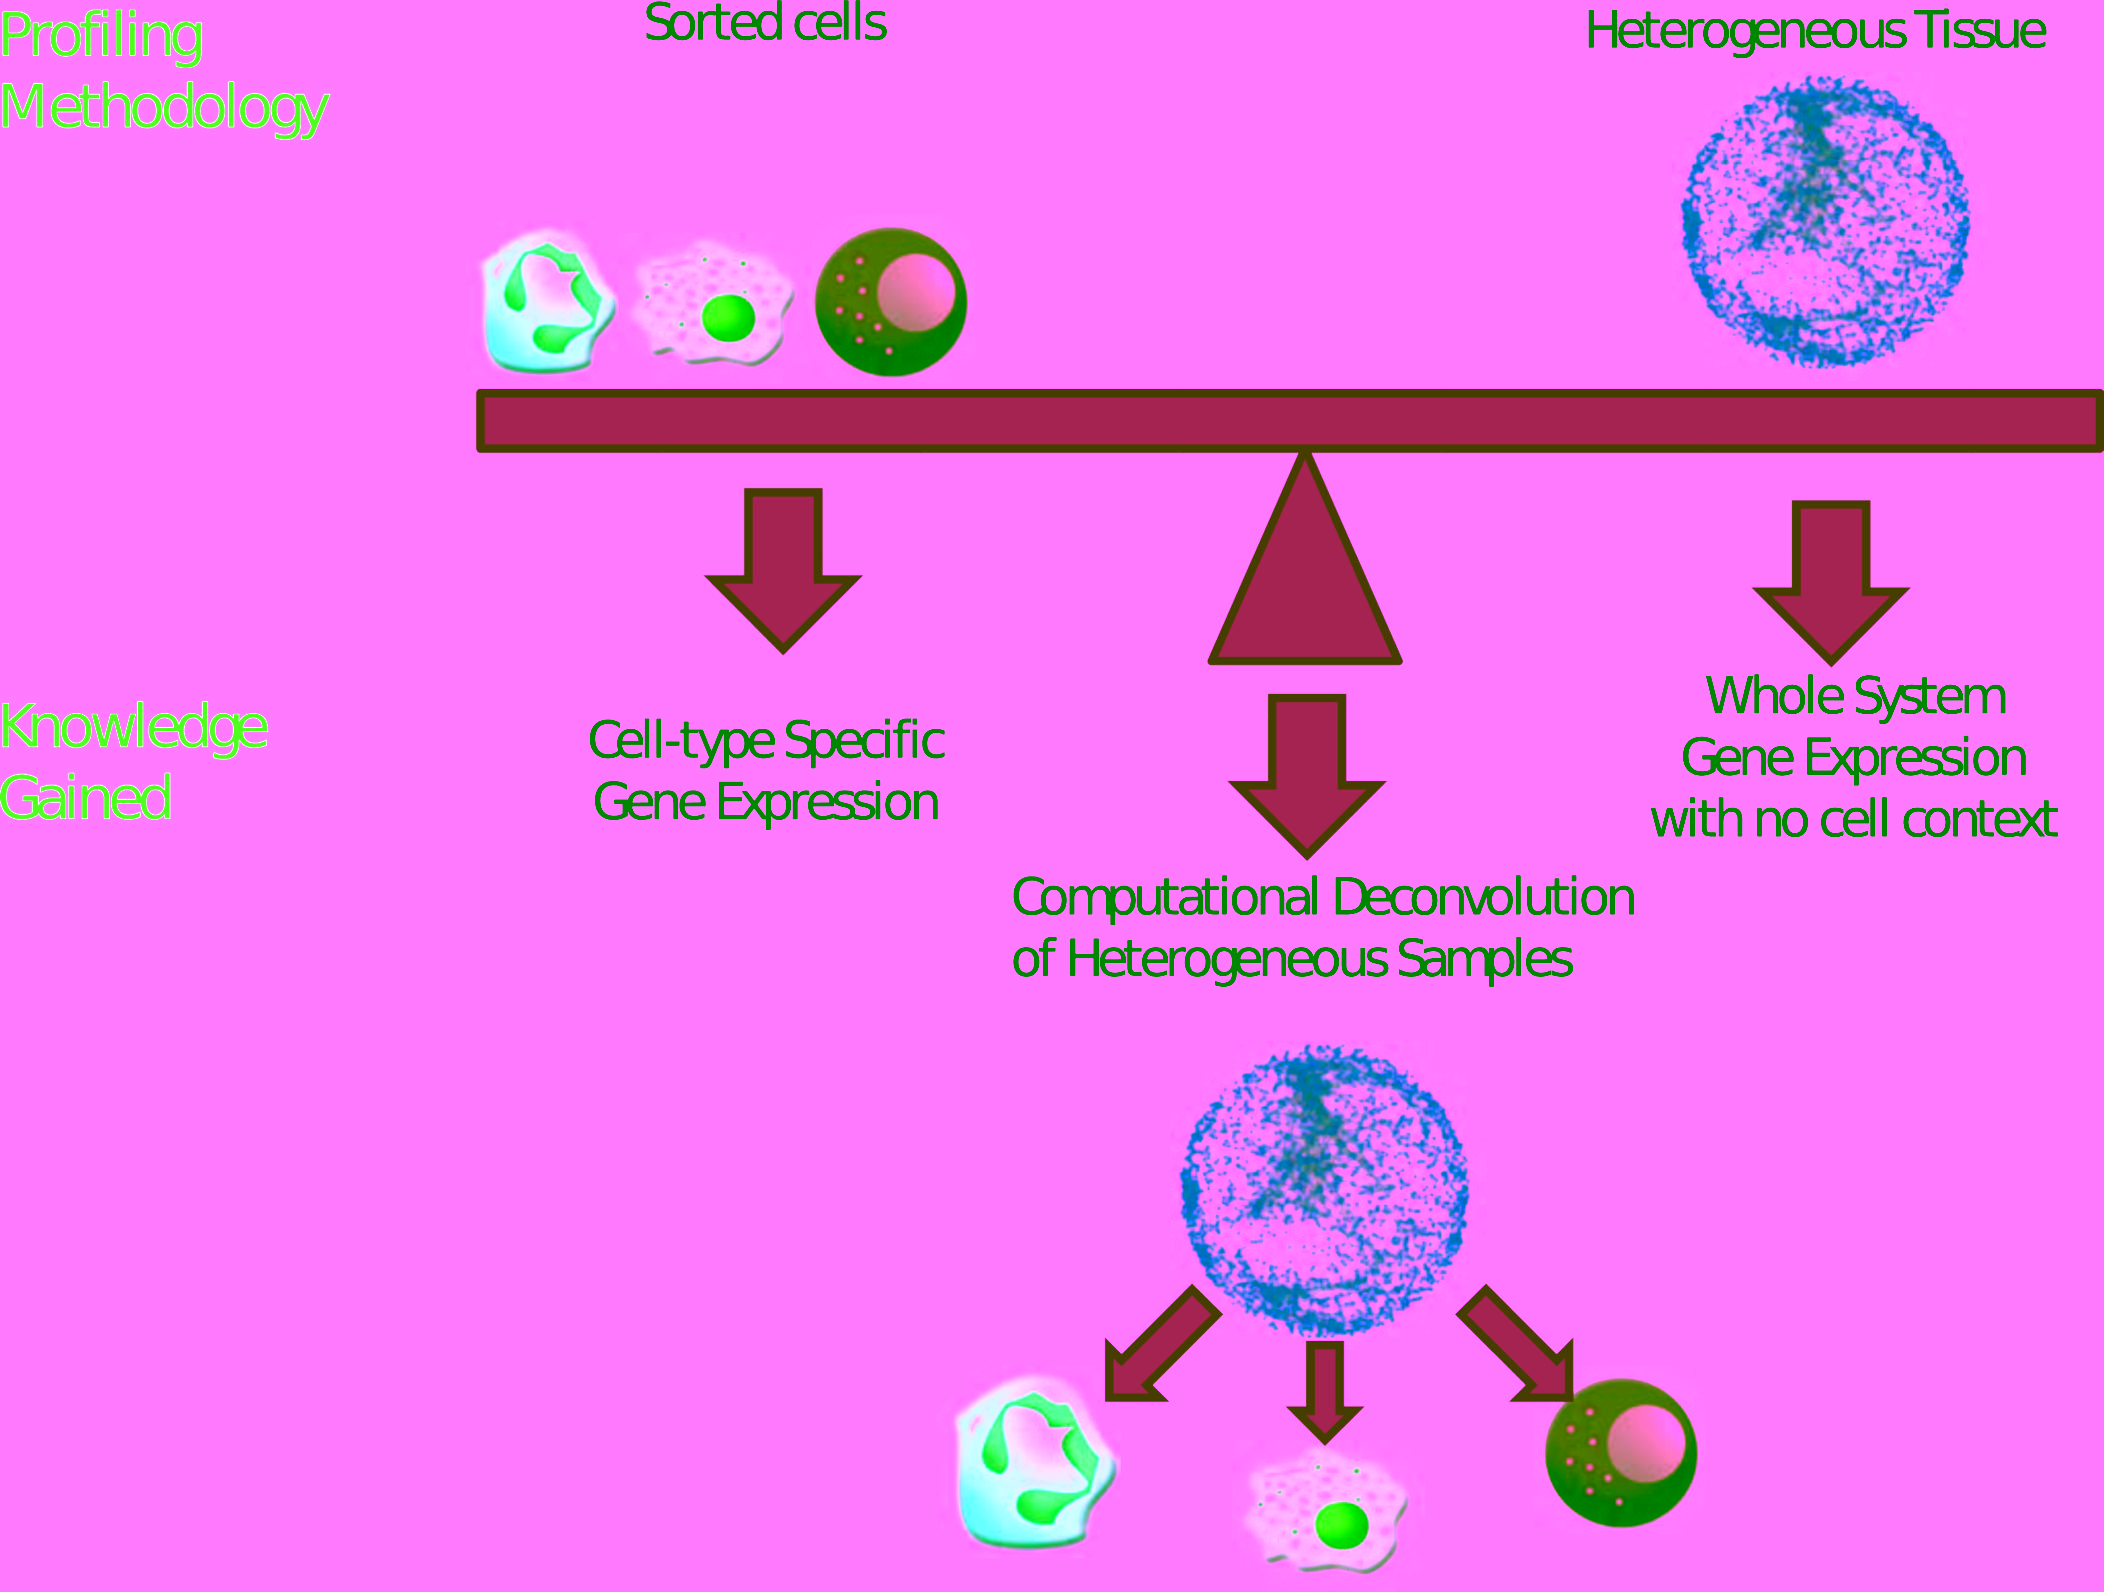
\includegraphics{figures/ShenOrr_2013_role_Computational_deconvolution.jpg}
%\caption{Computational deconvolution can capture both cell-centered and
%integrated biological network information}
%\end{figure}

\section{Physical methods}
\label{physical-method}


\subsection{Imaging methods}
\label{imaging-methods}

\emph{Immunohistochemistry}(IHC) \autocite{ju_etal13}, immune fluorescence (IF)
and in-situ hybridization (FISH-Flow, \autocite{kuhn_etal11}), as
opposed to the previous FACS method, enable an in-situ and so a spatial
characterization of the cell composition. They require tissue slides of
about one-cell width, such as FFPE samples, so that individual cells can
be visualized by microscopy at single-cell resolution. Individual cells
are first detected by segmenting the raw images, and then classified by
detecting signal emitted from the markers (can be present in nucleus,
cytoplasm or on within the membrane). To spot markers, both use a
combination of two antibodies: the primary one targets the cell marker
of interest while the secondary antibody, conjugated to either a
catalytic agent (IHC) or a fluorophore (IF), amplifies the signal. The
staining is then observed through a microscope and spatial
identification of the marked cell types is performed by pathologists or
with comparable performance by a deep deconvolution neural network. The
combination of different markers conjugated with a given antibody can be
used to unequivocally assign any stained cell to a specific population
\autocite{taube_etal18}.

Until recently, this methodology was limited to a small number of
markers due to the \emph{cross-reactivity} between primary and secondary
antibodies. The traditional way consists in staining consecutive tissue
slides with different antibodies. However, correctly realigning and
combining single slices is error-prone, losing the cell-cell distance
information. To overcome it, a recent methodology, the tyramide signal
amplification (TSA) system, allowed to increase the number of markers to
seven colours that could be stained simultaneously. In this system, TSA
free radicals catalysed by conjugation of the horseradish peroxidase to
the secondary antibody allows isolation of the complex formed by the
primary and secondary antibodies. It decreases then the risk of antibody
cross-reactivity when adding new antibodies to stain distinct markers.
In contrast to other methods, the multiplexed analysis of several
markers reveals in detail the anatomical structure, including cell
types' location, detection of lymphoid structures or formation of blood
vessels related to angiogenesis Lim et al.
\autocite{lim_etal18}.

%\begin{figure}
%\centering
%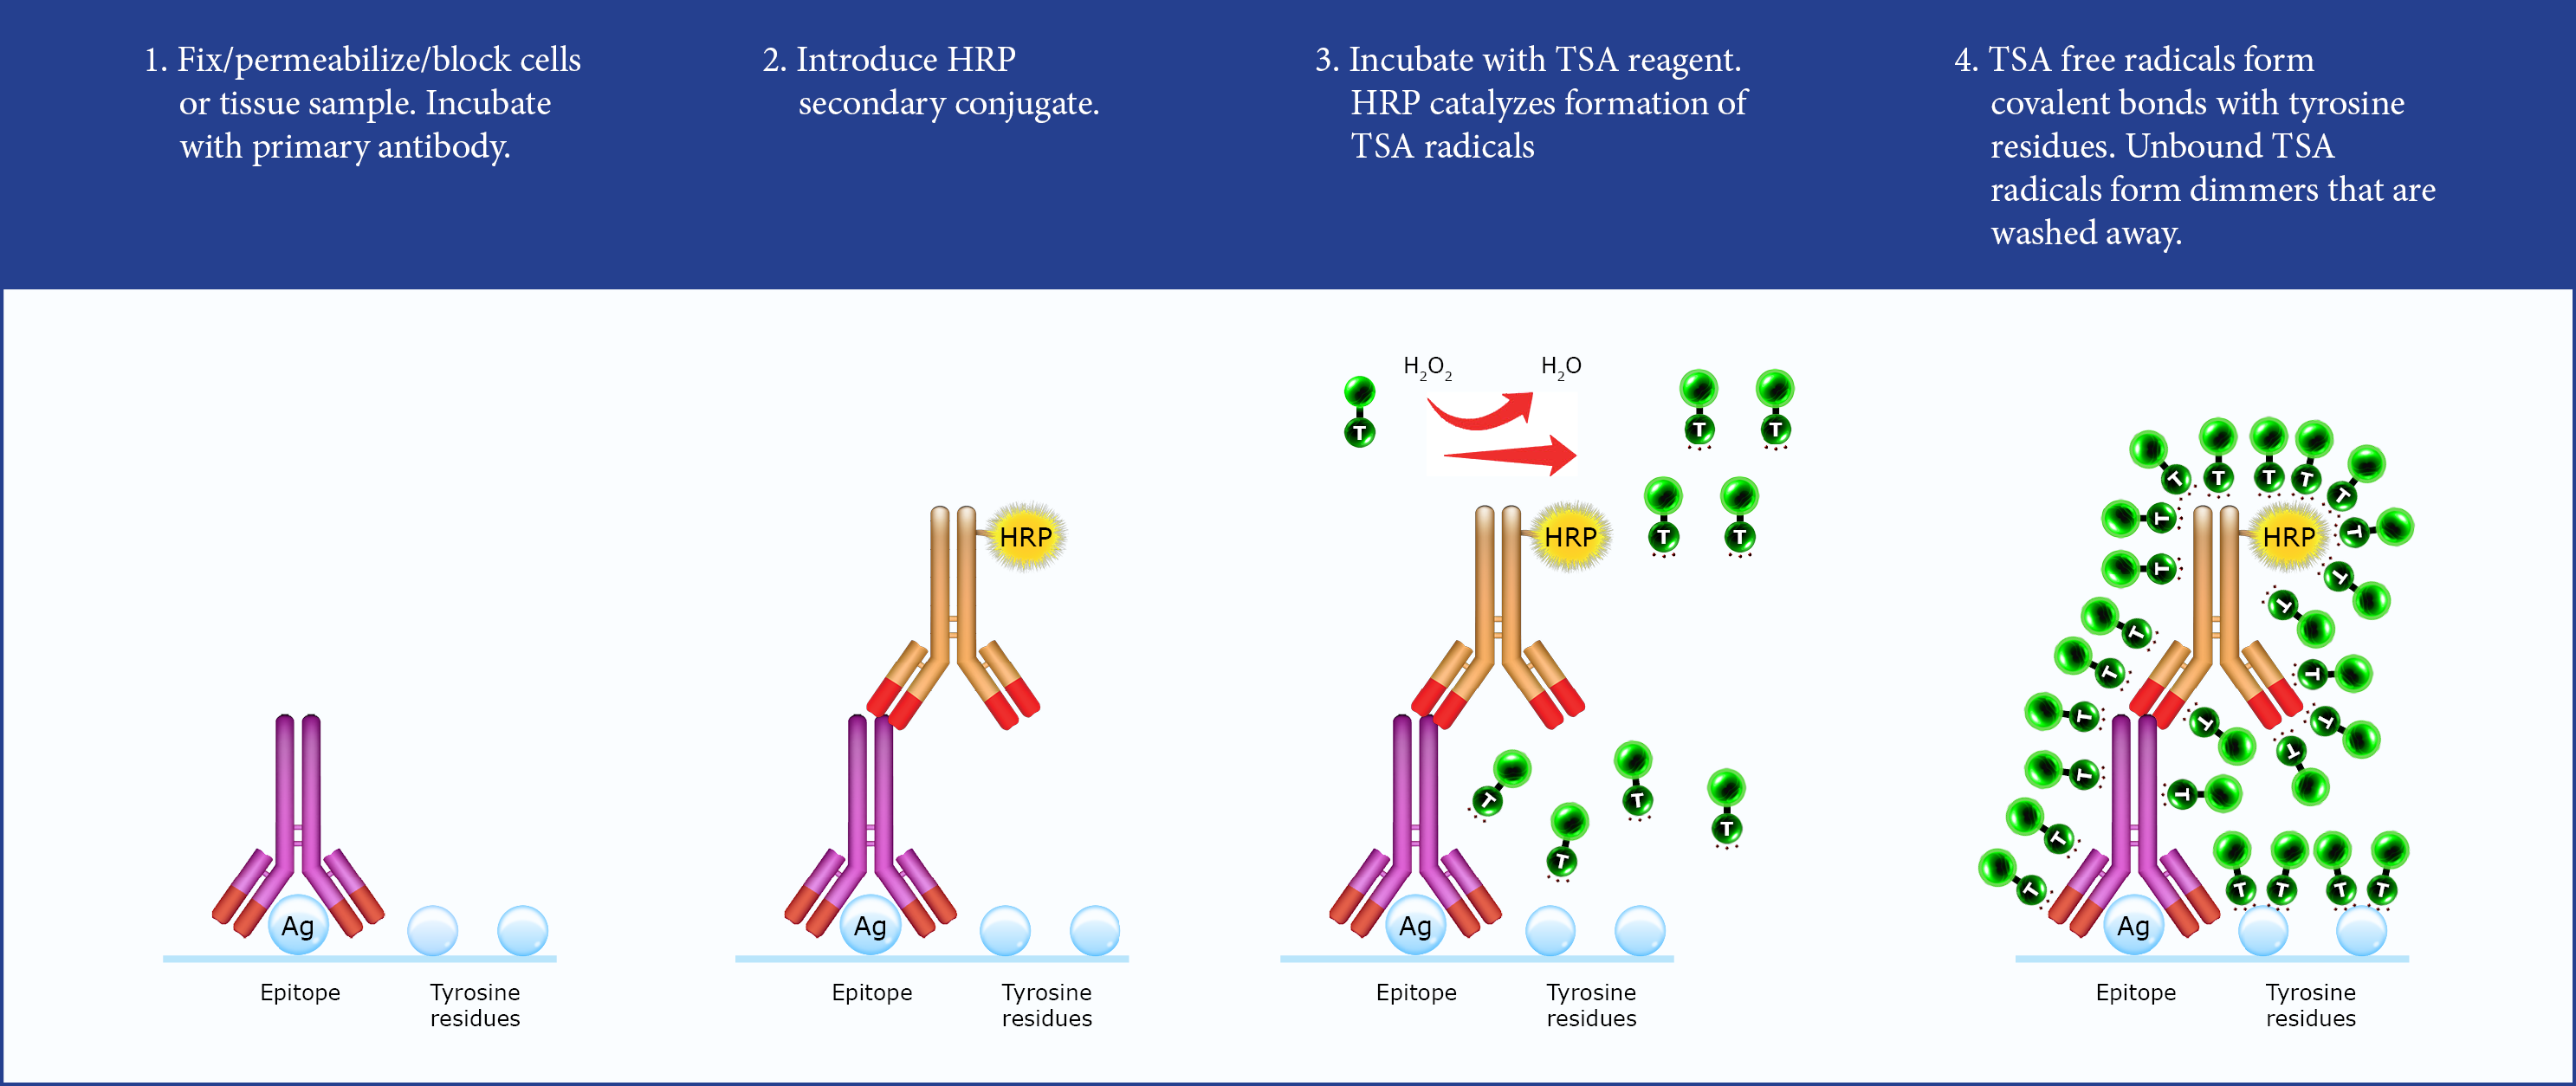
\includegraphics{figures/TSAWorkFlow.png}
%\caption{Description of TSA methodology}
%\end{figure}

Other IF-based methods that use a combination of sequential staining
with innovating staining approaches to enable highly multiplexed
quantification of biomarkers include cyclic immunofluorescence (CycIF)
\autocite{lin_etal15}, multiplexed immunofluorescence
(MxIF)\autocite{gerdes_etal13} and
multiepitope ligand cartography (MELC)
\autocite{schubert_etal06}. They
use photobleaching to stop cell fluorescence from the previous marker
and can stain 100 markers in a row. Finally, combination of mass
cytometry with IHC enable to get a deeper resolution at the subcellular
level (imaging mass cytometry (IMC)
\autocite{giesen_etal14}, Multiplexed
ion beam imaging: MIBI 33). Nonetheless, both technologies require heavy
instrumentation, with a weak throughput. Finally, a simpler technique named CODEX was
recently developed \autocite{goltsev_etal18} that requires less material to perform the analysis.

In-situ methods provide relevant yet highly dimensional data, with
information at single-cell level, including spatial coordinates and
staining intensities of the expressed markers up to the cell's
cytoskeleton. Spatial coordinates of the cell types can thus help to
detail the tumour immune landscape, for example, the cell-cell distances
yield information about the tumour immune architecture (vicinity of the
immune cell types) and so the tumour--immune cell interactions along
with their chronological evolution. To analyse this data, a similarity
matrix is built, representing the distances between two cell expression
profiles. Then, to interpret it, several dimensionality reduction
methods, such as t-SNE \autocite{maaten_hinton08} (non-parametric, unveil local structures) and UMAP (preservation of global distances)
\autocite{becht_etal19}, have been developed to reveal the
intrinsic non-linear structure of the single-cell data. Yet,
optimization of their hyper parameters, keeping both local and global
layout, is a complex task, and clustering of such 2D-projected plots may
be improved by accounting explicitly for the data sparsity
\autocite{pierson_yau15}. To
interpret the projections, instead of grouping cells with similar
expression profiles as homogeneous clusters, we may consider the recent
biological hypothesis that state of a cell is a continuum and that it
evolves dynamically throughout states, playing a key role on the
plasticity and so the ability of the immune system to respond quickly
and specifically to new pathogens or neoantigens. Graph-based approaches
can be used to infer linear and branched pseudo-temporal trajectories
that groups together cells emerging from the same lineage. Then, a
minimum spanning tree, or any other graph construction, some borrowed
from topological algebra, can be used to build a chronological timeline
of the cell state transitions, e.g.~the transition from naive to
cytotoxic CD8+ T cells. This estimated 1D ordering of time reference is
referred to as pseudotime. However, automatic extraction of information
from whole-slide images is still hampered by the numerous pre-processing
steps requiring manual interaction (such as defining the threshold to
discriminate unequivocally a marked cell type from background noise),
in-depth knowledge of image processing and extensive training of the
machine-learning algorithms. For instance, longitudinal single-cell
analysis helps disentangling the origin and the pseudo-time sequence of
distinct monocyte/macrophage states, with Monocle2
\autocite{qiu_etal17} revealing that
neither CX3CR1+ macrophages nor iNOS+ macrophages are present in the
early tumoral state.

\subsection{Cytometry analyses}
\label{cytometry-analyses}

Flow cytometry enables identification of populations at the single
level. To do so, the individual cells are isolated and then marked with
fluorophore-conjugated antibodies targeting markers of interest.
Identification of each cell's marker is performed by detecting the
fluorescence emitted back due to the simulation of a laser at a specific
wavelength. \emph{Gating}, namely the multiparametric expression of
various markers, can quantify precisely a large amount of single-cell
data (usually millions) within a large set of various population sets in
a relatively short time frame. The most recent FACS methods can quantify
up to 30 markers and 10,000 cells per second. FACS technics pioneered
the quantification of tumour-infiltrating immune cells, with early
description of dendritic cells (DC)
(\autocite{thurnher_etal96}) or
myeloid-derived suppressor cells (MDSC) (Veglia, Perego, and Gabrilovich
\autocite{veglia_etal18}).

\begin{figure}
\centering
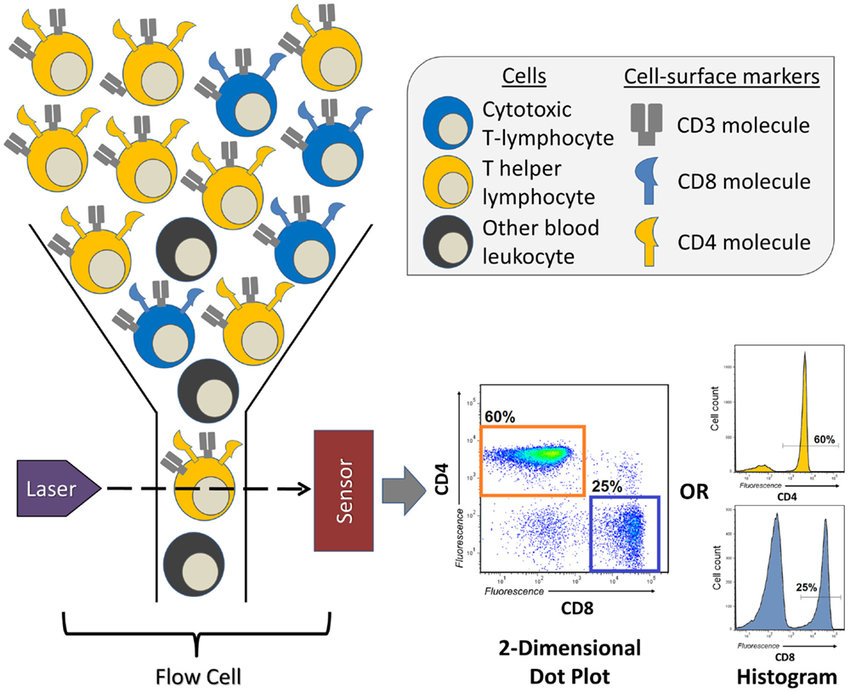
\includegraphics{figures/A-brief-overview-of-a-flow-cytometry-experiment-identifying-the-proportions-of-T-helper.png}
\caption{flow cytometry process}
\end{figure}

Initially, physical methods used to identify individual cells and hence
deduce their overall ratio in the biological sample were
Fluorescence-Activated Cell Sorting (FACS) or Laser Capture
Microdissection (LCM) technologies. However, these technologies require
specific cell-surface markers and corresponding antibodies to highlight
them. To overcome these limitations, novel systems relying on the
automatic discrimination of cell sizes by means of microfluidics or
dielectrophoretic separation were developed.

Of note, antibody-based methods require a known set of phenotypic
markers to uniquely identify cell populations, which might not be
available to set apart closely related cell population. As well, they do
not provide information about the functional state of specific immune
cells (no current consensus on single markers for determination of the
functional state e.g.~exhausted T cells)) and are biologically
intrusive, damaging cell structure (dead cells or doublets are not taken
into account). More specifically, FACS requires a large amount of
biological material while IHC provides only an estimate from a single
tissue slice.

To get a spatial insight on the transcriptomic activity, several
encouraging methods are developed to measure the expression of thousands
of genes in an antibody-free manner. This enables, using transcripts
instead of proteins, to characterize cells that can be identified only
accordingly to their transcriptomic activity. Two main classes of
methods use either hybridization (seqFISH+
\autocite{eng_etal19} and MERFISH
\autocite{chen_etal15}) or
sequencing (Spatial Transcriptomics
\autocite{stahl_etal16} and Slide-seq
\autocite{rodriques_etal19}). But
a compromise has to be found between the efficiency and the level of
accuracy required. SeqFISH and MERFISH enable subcellular resolution but
are low-throughput methods, while Spatial Transcriptomics can't achieve
single-cell resolution (\textgreater10 \(\mu m\)) while FISSEQ has a
high detection threshold (\textgreater200 mRNA molecules per cell).


\subsection{Single-cell technologies}
\label{single-cell-technologies}

The new Single-cell RNA sequencing ( \acrshort{scrna}) technologies are
promising to study rare populations, whose signal is usually confused in
bulk transcriptomics, and to get an insight on the intra-variability and
plasticity of the transcriptomic expression within a given population
\autocite{giladi_amit18}. First
step consists of isolating single cells, which can be done with plate-
(Smart-seq2, \autocite{picelli_etal13} via FACS technics or microfluidics-based (10X Chromium,
\autocite{zheng_etal17}) methods.
Microfluidics-based are less expensive, with higher throughput and can
thus profile a larger number of cells, but at the expense of lower
sensitivity. Then, each cell transcriptomic activity is individually
asserted. Besides, at the immune level, paired associations of the
\(\alpha\)- and \(\beta\)- chains forming the TCR determine together
their antigen specificity and are only kept at the single-cell level
resolution, along with the interaction between the immune population and
its functional state.

CyTOF \autocite{nomizu_etal94} is an
alternative method for the analysis of single cells is, in which
antibodies binding to the cell-surface-expressed proteins enable
unequivocal identification of the cell type. Cell content is then
ionised in a plasma state and analysed using a quadrupole time-off-light
(TOF) mass spectrometer. A higher number of simultaneously stained
markers compared to classical FACS can be used for the cell
identification.

However, their development is hindered by their expensive costs, complex
protocols and lack of statistical tools to interpret their results.
Additionally, the identification and composition determination of the
cell population may be biased
(\autocite{lambrechts_etal18}) as
some cell types are more likely to be damaged, and thus their total
expression underestimated. Doublets can also bias the expression, as
paired cells captured together generate hybrid transcriptome that might
be falsely interpreted as intermediate cell phenotypes. Indeed, the
primary step of single cell technologies requires a physical separation
and discrimination of the various cell subsets present in the sample,
subjected to the same artefacts and limitations of FACS methodologies.
Another main current limitation is the \emph{detection threshold} of the
transcriptomic signal, hindering detection of small transcriptomic
expression levels. This yields sparse transcriptomic expression
matrices, with numerous null expression values induced by
\emph{dropouts} due to the inefficiency of mRNA capture and the
stochasticity of mRNA expression. An additional challenge linked to the
peculiarities of these data is its intrinsic high dimensionality, with
higher noise and absence of biological replicates per sample. Finally,
annotation of the cell types is crucial but currently no consensus on
how to systematically identify known and novel cell types has been
established. Indeed, classical unsupervised clustering approaches split
the data into discrete clusters while cells are present in a continuum
of states, are sensible to the parametrization and might not identify
small clusters composed of rare cell populations. Accordingly, in most
of the  \acrshort{scrna} studies published so far, cell annotation is still
performed manually. A comparison between bulk and \acrshort{scrna} is illustrated below, in \Cref{fig:scrna-vs-bulk}.

\begin{figure}
\centering
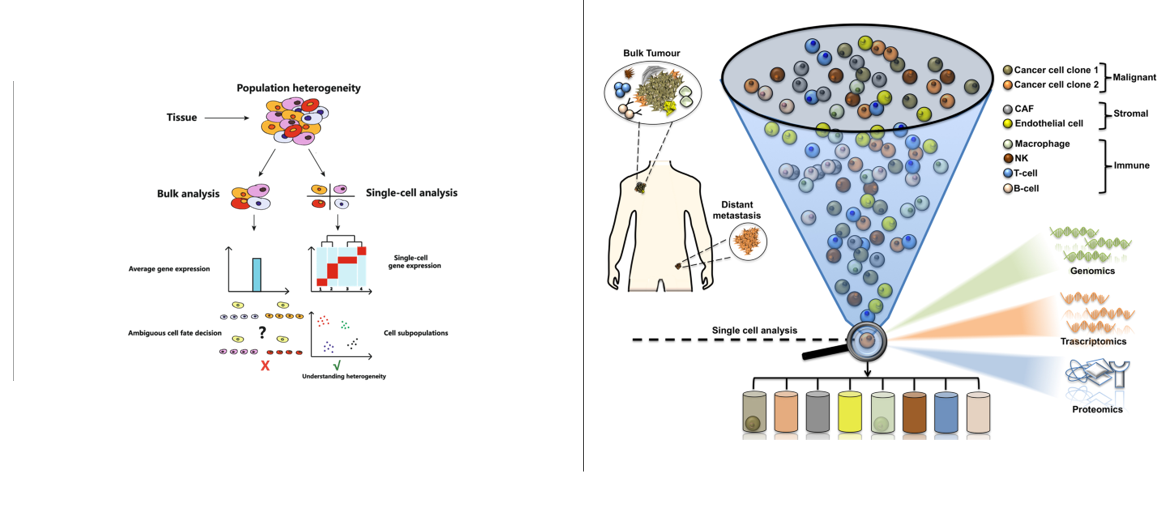
\includegraphics[width=0.8\textwidth]{figures/single_cell_methodology.PNG}
\caption{ Single-cell RNASeq pipeline compared to bulk transcriptomic RNASeq}
\label{fig:scrna-vs-bulk}
\end{figure}



A systematic and comparative review of the respective performance of these methods is summed up in \Cref{fig:mse-complex_heatmap}

\begin{figure}
    \centering
    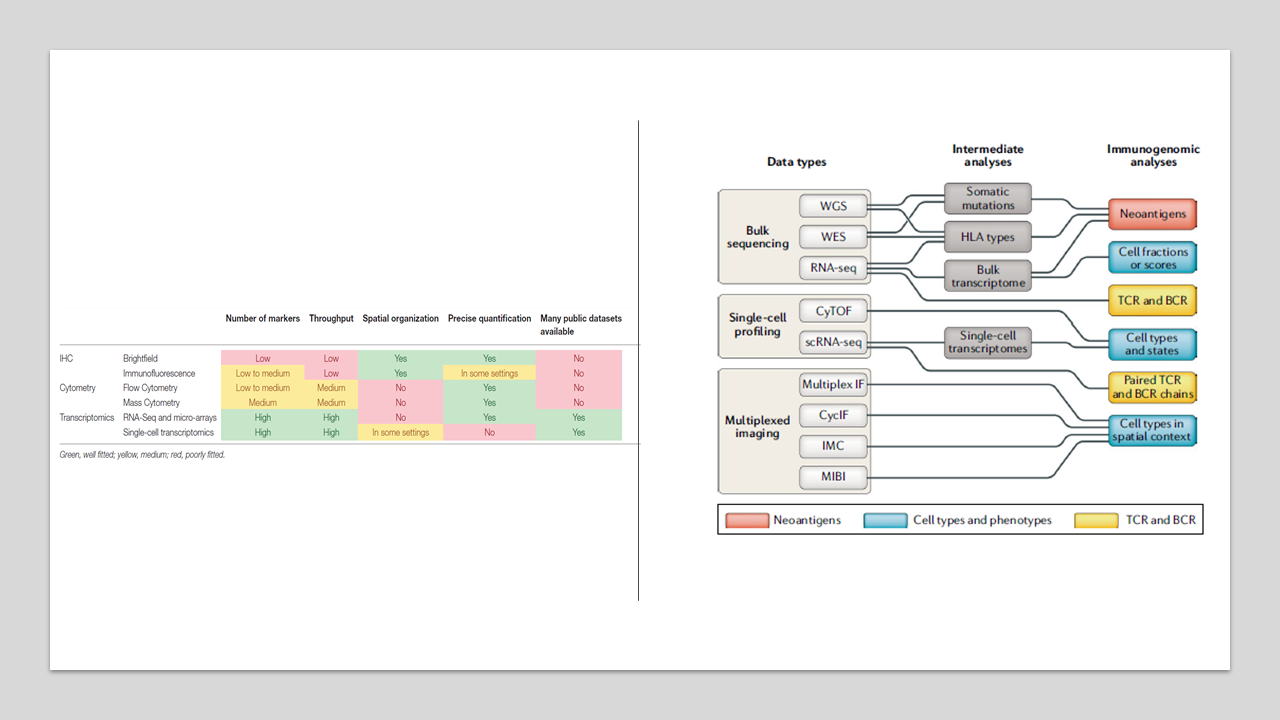
\includegraphics[width=0.5\textwidth]{figures/tme_estimation_technics.PNG}
    \caption{Comparison of accuracy and sequencing throughput of the most commonly used methods to decipher the biological medium, reproduced from \autocite{finotello_trajanoski18}}
    \label{fig:mse-complex_heatmap}
\end{figure}



\section{Computational methods using transcriptomics data}
\label{computational-methods-using-transcriptomics-data}

To overcome the highly costs of  \acrshort{scrna} technologies and exploit old
relevant bulk data (re diseases, long follow-up studies or complex
tissue extraction) for which the biological samples may not be available
anymore, multiple computational approaches have been developed in the
past years to infer ratios of cell types in biological
samples\autocite{avilacobos_etal18}. Additionally, single cell technologies, by physically separating
the various cell populations present in a biological sample, may hinder
the complex interactions within them, while computational techniques,
extracting directly cell-specific information from heterogeneous
samples, capture both cell-centered and whole-system information
landscape.

\emph{Deconvolution} generally speaking names the process that consists
in retrieving from a mixture its individual subcomponents. Linear
deconvolution is a subproblem of the general problem of the blind signal
separation, popularized as the `cocktail party problem'
\autocite{cherry53}. In a biological sample
(whole blood, tissue, \ldots), this consists generally in retrieving the
distinct cell populations (immune, stromal\ldots) composing it, but it
can be directly extended to identify the different sources of the RNA
production (for instance, many studies investigate on estimating a
tumour purity score returning the proportion of malignant cells in \autocite{yoshihara_etal13})
or set apart distinct cell phases. General pipeline is briefly described below \Cref{fig:cibersort-pipeline}

\begin{figure}
\centering
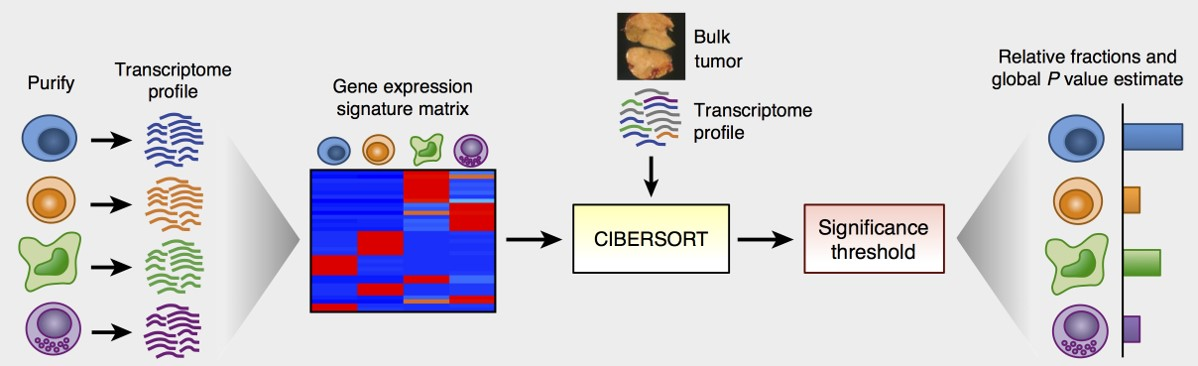
\includegraphics[width=0.7\textwidth]{figures/deconvolution_general_process.jpg}
\caption{Cibersort general description}
\label{fig:cibersort-pipeline}
\end{figure}

\todo{Use our own infography}

In classic linear deconvolution analyses, the gene expression measure is
the sum of each cell populations' gene expression weighted by their
corresponding proportions. If we consider a 'perfect' measure (no noise,
all cell types correctly identified, \ldots), we can be describe the
model as such:

\[
y_i = \sum_{j=1}^k x_{ij} \times p_j
\] 

with \(y_i, \quad 1 \le i \le n\) the sample's bulk transcriptome measure of gene \(i\), generated by \(k\) distinct cell populations
described by their proportion in the mixture \(p=p_{1:m}\) and their
individual specific expression \(x_{i, j}\), with \(1 \le j \le k\)
index of the cell population. Such equation states that the bulk gene
expression is the sum of individual cell specific expression \(x_{i.}\)
weighted by the proportion \(p_j\) of the cell population in the sample.
Additionally, the following constraints are generally applied on the model: 

\begin{equation}
\begin{cases}
\sum_{j=1}^J p_j=1\\
\forall j \in 1, \ldots, J, \quad p_j\ge 0
\end{cases}
\label{eq:simplex-constraint}
\end{equation}

 stating that no other cell population is present in the sample, and
that cell ratios must logically be non-negative values. For the ensemble
of \(n\) genes, this can be represented matricially by the following
equation: 
\[
y=\mathbf{X}p
\] 

Finally, let \(S\) the number of measured samples (in possible
distinct individuals, or in different tissues or at distinct period of
times in the same individual). The transcriptomic expression is then
given by a \(n \times S\) matrix, whose
\(s^{\text{th}}, \quad 1 \le s \le S\) is the transcriptome of sample
\(s\). Then the transcriptomic matrix \(\mathbf{Y}_{1:n, 1:S}\),
assuming that the expression of a population cell type is
\emph{tropic}-free (same no matter the individual or tissue) verifies
the following matricial equation: \[
\mathbf{Y}_{1:G, 1:N}=\boldsymbol{X}_{1:G, 1:J} \mathbf{p}_{1:J, 1:N}
\]

\[
\begin{pmatrix}
y_{1, 1} & \ldots & y_{1, N}\\
\vdots & \ddots & \vdots \\
y_{G,1} & \ldots & y_{n, N}
\end{pmatrix}
=
\begin{pmatrix}
x_{1, 1} & \ldots & x_{1, J}\\
\vdots & \ddots & \vdots \\
x_{G,1} & \ldots & x_{G, J}
\end{pmatrix}
\times
\begin{pmatrix}
p_{1, 1} & \ldots & p_{1, N}\\
\vdots & \ddots & \vdots \\
p_{J,1} & \ldots & p_{J, N}
\end{pmatrix}
\] where \(p_{j, s}\) is the proportion of the cell population \(j\) in
sample \(s\). Several information can be extracted from cell
type-specific analysis, to detect signal of a cell type in a mixture,
going further by estimating either its proportion or specific expression
profile or in a totally unsupervised manner, identify possibly new cell
populations by retrieving both individual signal and ratio of the
mixture. These four general information are summed up in the following
picture, and we describe in further details in next section main
technics used to do so.

%\begin{figure}
%\centering
%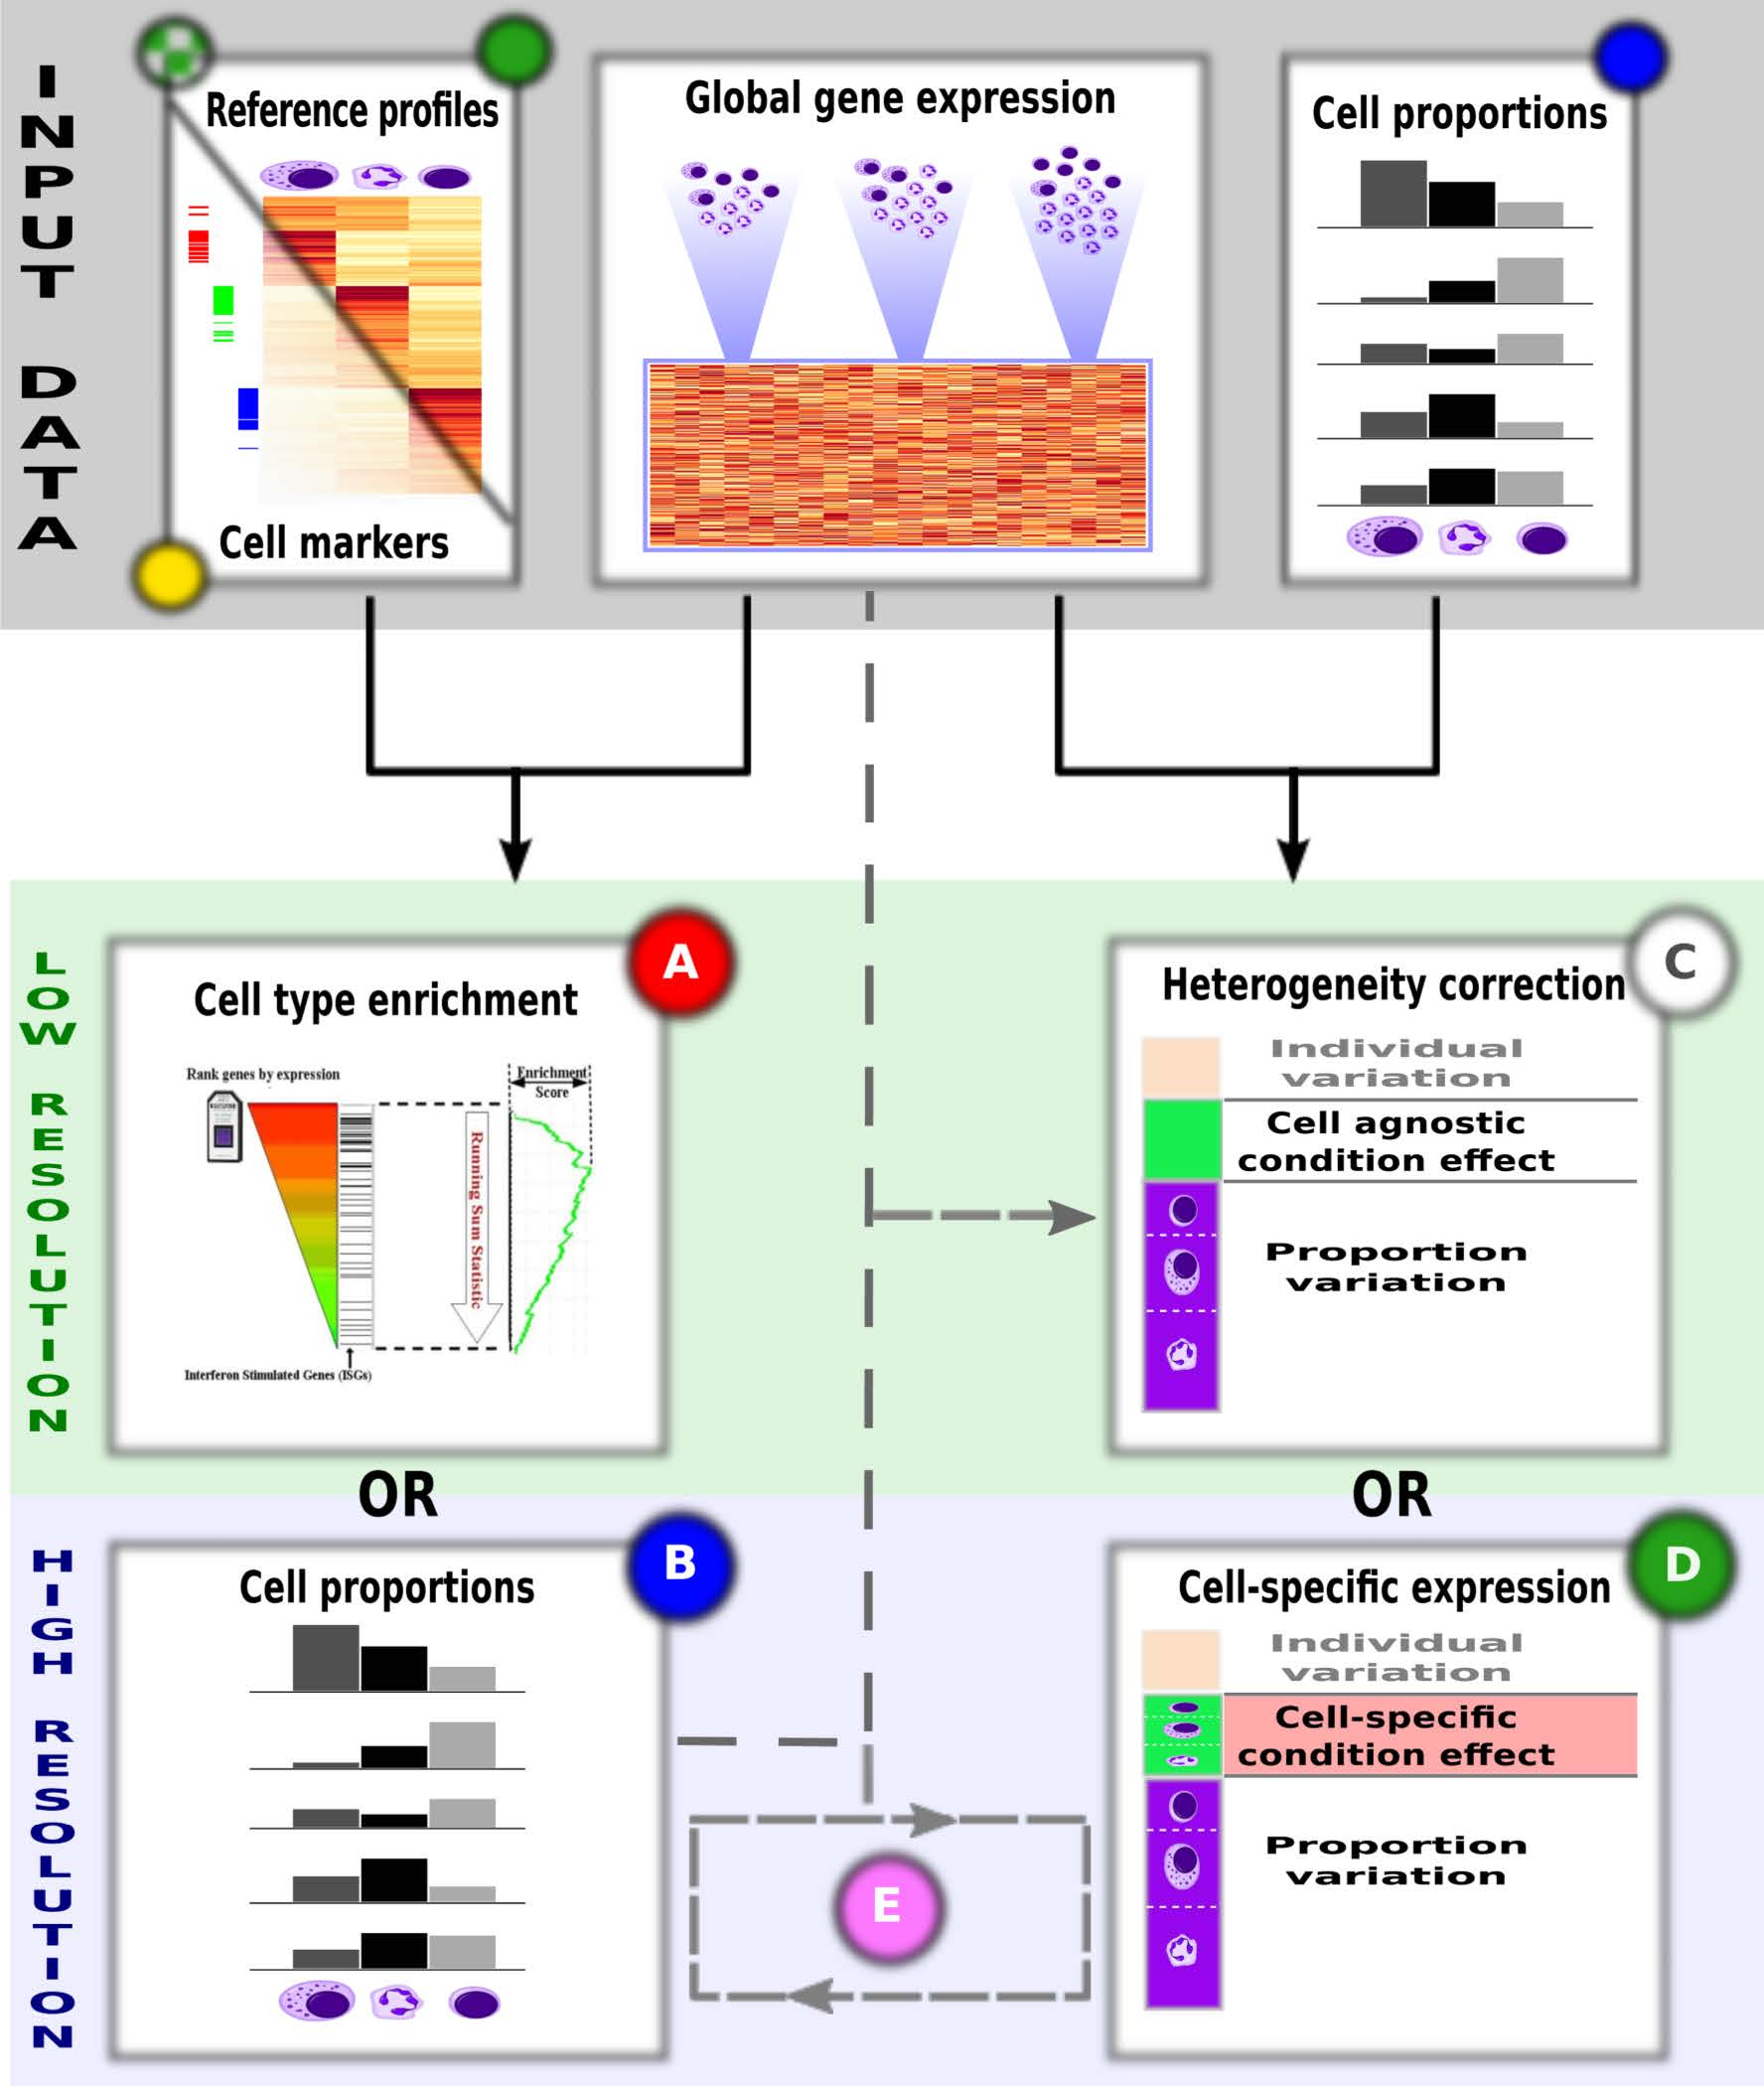
\includegraphics{figures/shenorr_purposes_deconvolution.jpg}
%\caption{Main purposes of computational deconvolution}
%\end{figure}


\subsection{Partial deconvolution technics}
\label{partial-deconvolution-technics}

Most published methods, referred as partial deconvolution methods, rely
on the measurement of cell proportions to estimate population specific
expression profilesStuart et al.
\autocite{stuart_etal04}, or on the measurement of
specific expression profiles to estimate proportions.


\subsubsection{Estimate the ratios}
\label{estimate-the-ratios}

In a perfect system without noise as modelled in equation {[}{]}, the
number of solutions, with \(p\) the unknown variable vector to estimate,
is given by the ``Rouché--Capelli'' theorem
\autocite{shafarevich_remizov13}. Briefly, uniqueness of the solution implies that the number of
genes \(n\) is equal to the number of cell types studies \(k\), and that
the expression of an individual gene can not be rewritten as a linear
combination of the remaining genes expressed in the sample (matricially,
this implies that the reference matrix \(\boldsymbol{X}\) is invertible).
When the number of genes exceeds those of cell populations, the system
gets overdetermined, and solution to the corresponding system of
equations, without collinearity in the gene observations, requires to
account for noise in the deconvolution problem.

According, goal of the ordinary least squares method (OLS) is to
minimize the sum of squares (SSE) between fitted values:
\(\hat{y} = \boldsymbol{X}\hat{p}\) and observed values: \(y\), regardless
of the distribution of the error term: \[
\hat{\mathbf{\epsilon}} = ||\hat{y} - y||^2 = ||\boldsymbol{X}\hat{p} - y||^2 = \sum_{g=1}^G \left( y_g - \sum_{j=1}^J \hat{p_j} X_{ij}\right)
\] The OLS estimator,\(\hat{p}_{\text{OLS}}\), that minimizes the sum of
residuals above, is given, using the normal equations, by: \[
\hat{p}_{\text{OLS}} = \arg \min_{\hat{p}} \left( ||\boldsymbol{X}\hat{p} - y||^2 \right) = (\boldsymbol{X}^T\boldsymbol{X})^{-1}\boldsymbol{X}^Ty, \quad y \in \mathbb{R}^n, \boldsymbol{X} \in \mathbb{R}^{n \times k}, p \in \mathbb{R}^k
\] \[
\hat{\mathbf{p}}_\text{MLE} = \arg \max_{\mathbf{p}} \left( \mathbb{P}_\mathbf{p} (y_{1:G}|\boldsymbol{X}_{1:G, 1:J})\right)= \arg \max_{\mathbf{p}} \left( \prod_{g=1}^G  \mathbb{P}_\mathbf{p} (y_{g}|\boldsymbol{X}_{.g})\right) \text { with } y_{1:G} \sim \mathcal{N}_G(\boldsymbol{X} \mathbf{p}, \sigma^2\mathbf{I}_G)
\] We generally assume a null spherical multivariate Gaussian
distribution for the distribution of the noise, a.k.a. the \emph{error
term}
\(\mathbf{\epsilon} \sim \mathcal{N}_n (\mathbf{0}, \mathbf{\Sigma})\),
with a \(n\)-zero mean vector and a diagonal covariance matrix of
constant diagonal term corresponding to the variance on the gene
measure, \(\mathbf{\Sigma} = \sigma^2 I_n\). The form of the covariance
matrix induces several assumptions on the biological model:

\begin{itemize}

\item
  \emph{weak exogeneity} the cell type-specific expression profiles are
  considered as fixed values and not random variables. This erases the
  intra-variability of a given gene within a cell population.
\item
  \emph{constant variance} as homoscedasticity, meaning that the
  variance is the same for any observation, in other terms, that
  \(\text{var} \left(\epsilon_i\right)=\sigma^2, \quad \forall i =1, \ldots, n\)
\item
  \emph{independence of the errors},
  \(\quad 1 \le i \le n, \quad 1 \le j \le n, \forall i \neq j, \quad \text{cov} (\epsilon_i, \epsilon_j)=0\),
  implying biologically that the bulk gene expression measured is
  independent of the others
\item
  the null expected value of the error term,
  \(1 \le i \le n, \quad \mathbb{E}(\epsilon_i)=0\), implying
  biologically that only the cell populations referenced in the
  signature matrix are responsible for the observed transcriptomic
  expression.
\end{itemize}

To avoid redundancy and guarantee the uniqueness of the solution, the
reference matrix \(\boldsymbol{X}\) must be of full rank \(k\), implying
that the number of gene observations \(n\) is superior to the number of
cell ratios to be estimated \(k\), and that no cell population specific
expression can be written as a linear combination of the others
(multicollinearity). The lowest variability on the estimate is obtained
when cell expression profiles are uncorrelated to each other, a strongly
assumption that might be only valid at a high level of the cell lineage.

With the conditions listed below, we can apply the
\emph{Gaussian-Markov} theorem, stating that the OLS estimate is not
only the unique estimate returning the global minimal of equation
{[}{]}, but the BLUE estimator (best linear unbiased estimator),
i.e.~the unbiased estimator (in average, no difference between the
estimated parameter and its true value) with the lowest variance. Except
when the number of ratios to estimate is rather small (and so the
columns of reference matrix profile), the direct computation of the
reverse matrix \((\boldsymbol{X}^T\boldsymbol{X})^{-1}\) is a rather difficult
task, proned to numerical rounding errors. Instead, \(QR\)
decomposition, in which the rather difficult reference matrix
\(\boldsymbol{X}\) is decomposed as the product of \(\mathbf{Q}\), a
\(n \times k\) orthogonal matrix, and \(\mathbf{R}\), a \(k \times k\),
upper triangular matrix, is often favoured. The OLS estimator is then
given by: \(\hat{p}_{\text{OLS}} = \mathbf{R}^{-1} \mathbf{Q}^T y\),
where the triangular matrix \(\mathbf{R}\) is much easier to invert.
Additionally, in the LLS method, linearity is only required with respect
to the coefficients of the model \(p\) with a possibly nonlinear
transformation of the bulk transcriptome \(y\) and gene reference
profile \(\boldsymbol{X}\): \[
\psi'(y_i)= p_0 + \sum_{j=1}^k p_j \psi_j(X_{ij})
\] with \(\psi\) a possibly nonlinear function. Usual transformation is
the TPM normalization for \acrshort{RNA-Seq} data that enforces a fixed measured
quantity of RNA transcripts for each sample. As shown in
\autocite{racle_etal17}, TPM
normalization being a linear function ensures that if the sum of the
estimated ratios in raw data sums to one, then the TPM normalized
estimated ratios comply this condition. Another rarer function used is
the \emph{log2} transformation
\autocite{hoffmann_etal06},
supposed to guarantee better the normality conditions of the residuals
required by the Gaussian Markov theorem. However, this model has no
biological sense, with no sum-to-one constraint preserved.

This \emph{linear model} is the one used in
\autocite{abbas_etal09}
paper, using the R \emph{lsfit} function, to estimate 18 different
immune cell ratios. They show that the activation of NK and T helper
lymphocytes were highly correlated to symptoms of the SLE disease, with
a prominent impact on the interferon signature. But it is sensitive to
outliers and efficiency of the estimate relies on a set of strict
conditions that aren't usually met in biological conditions,
e.g.~homoscedasticity of the residuals and absence of correlation
between the residuals and observed values. Additionally, the OLS
estimated ratios might be negative or not sum-to-one, having no
biological sense. Hence, such coefficients are artificially removed
after the estimation. The same method is used in
\autocite{li_etal16}, in a context of
tumoral mixture. To avoid accounting for tumoral cells when asserting
ratios of infiltrated cells, only genes both highly correlated to the
cell types of the sample and negatively correlated to the \emph{tumour
purity} are integrated in the reference matrix. In this study, tumour
purity is the ratio of \emph{aneuploid cells}, namely cells with a non
canonical number of 46 chromosomes, asserted by the CHAT (clonal
heterogeneity analysis tool) R package (not maintained anymore on the
CRAN), considered as surrogate variable of the true ratio of tumoral
cells. Additionally, a pre-filter on the top \(1%
\) most varying genes is performed to maintain the heteroscedascity
assumption. This study identifies 2 subgroups of melanomas with two
distinct levels of TCD8 subsets, and associated to distinct prognostic
issues.

The sum-to-one ratios might be relaxed, by integrating an additional
constant term accounting for remaining cell populations that might have
been left undetected. To do so, we simply need to add a column of ones
in the reference cell matrix is now:
\(\boldsymbol{X} \in \mathbb{R}^{n} \times \mathbb{R}^{k + 1}\), and
\(k + 1\) cell ratios are now estimated, \(p_0\) being the cell ratio of
uncovered cell subsets present in the mixture. Finally, a direct
approach, by adding weights proportional to the influence desired for
the gene expression measure on the OLS estimate, or indirect robust
approach adjusting automatically to outliers, can be used to account for
outliers in the mixture. In the weighted approach, the Weighted Least
Square estimate is given by
\(\hat{p}_{\text{WLS}} = (\boldsymbol{X}^T\mathbf{W}\boldsymbol{X})^{-1}\boldsymbol{X}^T\mathbf{W}y\)
with \(\mathbf{W}\) the diagonal matrix of weights, hence, the
individual error estimate with an intersection term is given by
\(\hat{\epsilon_i}=w_i\left( y_i - \hat{p_0} - \sum_{j=1}^k \hat{p_j} X_{ij}\right)^2\).
The weights are given by the user, low-quality points being associated
to small weights. In the robust approach, the weights are iteratively
adjusted till convergence (the usual prior being usually the uniform
weight for each observation), or, in a stricter way, some genes are
simply not used for the estimation.

CellPred, developed in \autocite{wang_etal10} for the estimation of stromal and tumour proportion from
microarray transcriptomic data, is an user-friendly web service that
performs a multivariate linear regression model with a noise intercept.
EPIC, \autocite{racle_etal17},
includes both processes, for the estimation of cell ratios in a tumoral
context. Instead of a constant term accounting for none described cell
population, the algorithm assumes that genes expressed in tumoral cells
are poorly transcribed in immune or stromal cells, and an additional
column corresponding to tumour is added to the reference cell
population. The signatures in EPIC were developed using both bulk and
 \acrshort{scrna}-seq data from circulating and tumour-infiltrating immune cells,
CAFs and epithelial cells, with one designed for whole-blood samples and
another for solid tumoral tissues. Besides, a weighted LLS method is
implemented to retrieve the ratios, with less weight given to highly
variable genes. It's worth noted that this method can be applied to
\emph{solid tumours} as the immune cells do not mix up with tumoral
cells, but not hematological malignancies (lymphonenia, leukemia\ldots),
where the estimated immune cell subset may be composed of a mixture of
both normal and mutated cells.

Same approach, but simply using a constant intersection term, is used in
the quanTIseq algorithm
\autocite{finotello_etal19}. To
integrate the drop-out observed in some cell subsets poorly present in
the sample and highly correlated to other cell types, they implement a
heuristic strategy averaging the estimated ratio of Tregs in presence
and in absence of the highly correlated \(TCD4^+\) subset in the design
matrix. QuanTIseq is specifically tailored for RNA-seq data and
implements a full analytical pipeline, from pre-processing of raw
RNA-seq data until deconvolution of cell fractions.

Actually, with gene expression data normalized per sample et cell
population, the estimated ratios \(\hat{p}\) returned by the
deconvolution method correspond actually to the fraction of mRNA coming
from each cell type, rather than the cell proportion itself. Dividing
the number of transcripts associated to a cell subset by the average
production of RNA transcripts (or equivalently the total weight of RNA)
yields the expected number of cells associated to this compartment.
Finally, the true cell population ratio derived from the RNA fraction is
given by: \[
\hat{p^*_j} = K \frac{\hat{p_j}}{r_j}, \quad K= \frac{1}{\sum_{j=1}^k \frac{\hat{p_j}}{r_j}}
\] with \(r_j\) the average number of transcripts extracted per cell
type, and \(K\) a normalization constant, such that the modified
estimated cell ratios still sum to one.

Post-correction of this biased effect is taken into account in
\autocite{racle_etal17} and \autocite{finotello_etal19}
studies, using the RNAeasy mini kit (Qiagen) to extract RNA nucleotides
a and a Fragment Analyser (Advanced Analytical) to quantify it in
\autocite{racle_etal17} paper and
using as a surrogate variable the expression of the housekeeping genes
in the Proteasome Subunit Beta 2 (PSMB2)
\autocite{eisenberg_levanon13} in \autocite{finotello_etal19} to retrieve 
the average number of transcripts \(r_j\). Still,
extraction efficiencies evaluated by both methods are high correlated.

Another similar interpretation of the \(r_j\) coefficient, as reported
in \autocite{liebner_etal14}, is the correction for technical bias with differential RNA
extraction efficiency whether the cell type. Unlike EPIC and QuantiSeq,
the MMAD (microarray microdissection with analysis of differences)
algorithm does not consider the coefficient extraction efficiency as
data provided by the user as input, but rather as a parameter to
estimate for the deconvolution algorithm, as well as the potential
biological perturbation induced by the phenotypical condition of the
sample. Then, the true estimated cell ratio can be decomposed, and
directly plugged in the LTS regression (ref equation): \[
\hat{p_{js}}^*= \hat{r_j} \hat{\beta_s} \hat{p_j}
\] In this case, the linearity between the response variable and the
weighted combination of the estimates is lost, and the LTS estimate is
computed using a non-linear conjugate gradient search algorithm,
implemented in MATLAB, with additional non-negative constraint on the
estimated parameters.

In the previously described approaches, all genes that were measured in
both the transcriptome \(y\) and the reference profile \(\boldsymbol{X}\)
were used for the deconvolution. However, such a an approach may yield
biased estimates, as the expression of some genes might significantly
differ between the bulk mixture and cell-separated subsets. Yet, these
outlying genes are the ones having the largest influence on the fit, due
to the squaring distance used to compute the error term.

Therefore, robust least-squares regression use only a subset of these
genes. To evaluate these methods, two metrics are generally used: the
relative \emph{efficiency} of the robust estimate, compared to the OLS
estimate when the assumptions of the Gaussian-Markov theorem apply (the
OLS estimate is indeed asymptotically efficient estimate, in the sense
of attaining the Cramér--Rao bound ), and the breakdown point (BP),
which is the minimal proportion of outliers in the dataset required so
that the estimate does not converge anymore. The OLS estimate has a
small BP of \(\frac{1}{n}\), implying that one single unusual
observation makes the estimation divergent
\autocite{rousseeuw85}. Several robust
methods, making a compromise between efficiency and robustness of the
estimate, were developed:

\begin{itemize}

\item
  M-estimate replaces the LLS criterion with a robust function of the
  residuals, giving less weight to highly leveraged points {[}{]},
\end{itemize}

\[
\hat{p}_{\text{IWLS}} =  \arg \min_{p} \sum_{i=1}^n \rho\left(\frac{y_i - \sum_{j=1}^k \hat{p_j} X_{ij}}{\hat{\sigma}}\right) = \arg \min_{p} \sum_{i=1}^n \rho\left(\frac{r_i}{\hat{\sigma}}\right)
\] 

where \(\psi = \rho'\) is the derivative of the robust function
\(\rho\), called the \emph{influence function}, for which the null
argument is the estimate to be found, and \({\hat{\sigma}}\) an estimate
of the residuals variability (sometimes the mean absolute deviation is
used), then \(\frac{r_{1:n}}{\hat{\sigma}}\) is the vector of
standardized residuals. With \(\rho(t)=\frac{1}{2}t^2\), we return on
the original OLS problem. Huber's function was the first used, in 1981,
with a strong smoothing as any absolute residual going beyond a constant
\(c\) (set to 1.345, the efficiency is \(95\%\) worth of the OLS
estimate) is given a null weight, while the same weight is given to any
other residual. Tukey's bisquare function is a soft smoothing function,
with the following influence function:
\(\psi(t)= \max \left(0, \left(1 - (\frac{t}{c})^2\right)^2\right)\).
Observations associated with a strong residual and so far the regression
line are given less weights, and the threshold gives null weight to
points that are farther from the regression line from what would be
expected by random chance. With c\(c=4.6885\) the efficiency of the
estimate is the same as Huber's estimate. With both functions, the
weights for each observation depend on the residuals that depend
themselves on the weighted estimator which itself is dependent of the
weights. As a result, the robust estimator must be computed iteratively.
The general process consists first in the initialisation step in
computing the OLS estimate, assuming uniform weights for any observation
(or any other weight returned by robust estimator, as in MM-estimates,
\autocite{yohai87}). Then, each observation
is weighted by the transformation of its corresponding residual value by
the influence function, and a weighted regression is performed, as given
in equation {[}{]}. When the weighted estimate converges, we stop this
iteratively reweighed least square regression. Although not described in
any deconvolution paper, the standard \emph{rlm} (for robust linear
modelling) function in the R MASS package, that performs the Tukey's
biweight iterative regression, is often implemented as a standard robust
method in any deconvolution benchmark paper. Another influence function
implemented is the Least absolute deviation (LAD), aka the \(L_1\)
estimate, that minimizes the absolute difference of the residuals,
instead of the squared differences:
\(\hat{p}_{\text{MAE}} = \arg \min_{\hat{p}} \left( |\boldsymbol{X}\hat{p} - y| \right)\).
Accordingly, extreme gene expression values \(y\) have less influence on
the regression. However, LAD can not be solved analytically, requiring
an iterative approach, such as the simplex-based Barrodale-Roberts
algorithm \autocite{barrodale_roberts73}. A LAD regression is performed in the RCR (robust
computational reconstitution) algorithm supplied in
\autocite{hoffmann_etal06}, in
which additionally trimming is performed (cf next point) and where the
non-negativity and the sum-to-one constraints are enforced. The final
number of genes used in their trimmed regression process corresponds to
the minimal number of genes to guarantee the uniqueness of the solution
(no matter the initial ratio estimates given in the initialisation
process, the same estimate is returned). Interestingly, they showed
theoretically that adding additional gene measures from the mixture at
that trimming point, that are more likely to be uncorrelated with gene,
leads to an artefact, with equal ratios attributed for each cell
population. All these methods remain sensitive to high leverage outliers
present in the cell reference matrix, and thus have the same breakdown
point as the OLS estimate. Additionally, they are less efficient in the
best case where the error is normally distributed, with LAD having the
lowest efficiency of 0.64 compared to the OLS estimate. - The LTS (least
trimmed squared) method was first proposed in
\autocite{rousseeuw85}, in which the
purpose is to find the \(q= n(1- \alpha) + 1\) observations, with
\(\alpha\) corresponding to the proportion of trimming, that have the
smallest residuals. Practically, the estimate is given by: \[
\hat{p}_{\text{LTS}} =  \arg \min_{p} \sum_{i=1}^q r_i (p)^2
\], with \(r_i (p)\) the residuals ordered by increasing order. LTS has
a strong BP of 0.5, taking \(\alpha=\frac{n}{2}\), making it strongly
resistant to outliers, but a very low efficiency of 0.08. LTS is an
NP-hard problem \autocite{rousseeuw85},
as any combination of \(\binom{n}{q}\) observations should be tested, to
find the \(q\) observations for which the estimate is minimal. With a
large number of observations, that's not computationally feasible, hence
\autocite{rousseeuw_vandriessen06} proposed a stochastic faster version of this algorithm,
in 2006. However, its performance is highly dependent on the initial
random \(q\)-subset chosen, and it's still too slow when the sample size
is too big, with initial bad initialization. Eventually, the number of
outliers to be trimmed has to be provided by the user. Accordingly, the
FARDEEP algorithm was developed by
\autocite{hao_etal19}, returning an
adaptive LTS estimate. At each step, the total number of points
considered as outliers is bounded between an overestimate and an
underestimate of the total number of outliers, with the series of
overestimate strictly decreasing and the sequence of underestimate
strictly increasing. Thus, the algorithm is guaranteed to converge in a
fixed number of steps, according to the hyperparameters provided by the
user. However, the algorithm is highly sensitive to the tuning parameter
\(k\) that indirectly controls the final number of observations trimmed
during the regression, and is not easily interpretable (the set of
outliers is composed of the observations for which the corresponding
absolute residual is above the median of the residuals multiplied by
\(k\)). And there's no theoretical result on the efficiency or even on
the consistency of the estimate returned, especially no guarantee to
find either the true number nor the set of outliers. A review of robust
linear estimates is supplied in \autocite{yu_etal14}, with 10 methods benchmarked, and in which
MM-estimates and REWLSE estimates have overall the best performance in
terms of robustness and asymptotic efficiency.

SVR (support vector regression) uses as well a specific metric keeping
the most informative gene expression, but rely on a different paradigm
than robust linear regression. As in classical linear regression, linear
SVR identifies the hyperplane that fits as many data points as possible.
But contrary to classical linear regression approaches, where all
observations are used for the fitting process, or to robust linear
approach, where distant points are trimmed or given less weight, the
most relevant gene expressions, referred as ``support vectors'' (SVs),
are the ones the most distant from the fitted hyperplane (in 3D, those
lying outside a tube of radius \(\epsilon\), centred on the fitted
hyperplane). SVs, penalized by a slack variable \(\zeta_i\) according to
their distance from the \(\epsilon\)-tube, define alone the linear
function, and any gene expression altered within the \(\epsilon\)-tube
would not impact the regression curve. Generally, the metric used in SVR
approach complies with the statistical learning principle stating that
in order to obtain a small risk, both the training error and model
complexity must be controlled. Hence, the optimization function consists
in \emph{a loss term} to be minimized (herein, the difference between
the estimated and observed transcriptomic values) and a \emph{penalty
term}, advocating for the model with the fewer coefficients.
Historically, the first SVR approach, \(\epsilon\)-SVR
\autocite{cortes_vapnik95}, uses
a \(\epsilon\)-insensitive loss function that automatically retrieves
the set of support vectors needed to reach the degree of precision on
the results required by the user. As suggested in
\autocite{cc_cj02}, this method is the
one recommended to reach the highest performances. CIBERSORT (Cell Type
Identification By Estimating Relative Samples Of RNA Transcripts), a
deconvolution algorithm developed in 2015 by
\autocite{newman_etal15}, uses a
more recent alternative, using a \(\nu-\) insensitive loss function,
that automatically determines the best precision that can be reached,
given as input the proportion of SV expected. Indeed,
\autocite{scholkopf_etal00} shows
asymptotically that the proportion of SVs returned correspond to the
\(\nu\) hyperparameter. The \(\nu\)-SVR primary optimization problem
tries to minimize the following risk function: \[
\min \left[ \tau (p, \zeta, \epsilon) = \frac{1}{2} \sum_{j=1}^k p_j^2 + C \left( \nu \epsilon + \frac{1}{n} \sum_{i=1}^l (\zeta_i + \zeta_i^* )\right) \right]
\] where \(C\) is a regularization parameter making the compromise
between penalizing for the complexity of the model and the fitness of
the model to the gene expressions. Additionally, the risk function is
subjected to the following constraints: \[
\forall i \in \{1, \ldots, n\}, \quad
\begin{cases}
(p x_i + p_0) - y_i \le \epsilon + \zeta_i \\
y_i - (p x_i + p_0)  \le \epsilon + \zeta_i^* \\
\zeta_i, \zeta_i^* \ge 0 \\
\epsilon \ge 0
\end{cases}
\] with \(p_0\) an inersection term. \autocite{cc_cj02} suggests that this method should be privileged for
reducing the complexity of the model (here, the number of gene selected
in the signature matrix). There's a direct relationship between the two
methods, as increasing the \(\nu\) hyperparameter and accordingly the
number of SVs used for the regression would result in a smaller
\(\epsilon\)-tube and a higher precision on the results. Additionally,
the values of the estimated ratios using \(\nu\)-SVR associated to a
specific degree of precision \(\hat{\epsilon}\) has the same solution
than \(\epsilon\)-SVR, fixing a priori the degree of precision to be
reached at \(\epsilon\). The \(L2\)--norm penalty function (the same as
used in ridge regression) penalizes model complexity by penalizing the
variance associated to the estimated ratios corresponding to highly
correlated cell-types, while the \(\nu\)-insensitive function avoids
over-fitting by only selecting and penalizing the most leveraged points,
making it less sensitive to noisy samples
\autocite{cherkassky_ma04}.
Indeed, ``spillover effects'' (when contribution of a cell type is
masked by the noise magnitude or another cell type highly correlated),
are efficiently tackled with SVR approach, enabling them to integrate
more distinct cell types in their analysis. No physical constraint of
non-negativity on the estimated ratios is enforced, hence,
non-negativity and sum-to-one constraints on the SVR-estimated ratios
are applied afterwards (as done in the OLS method provided by
\autocite{abbas_etal09}).
Oddly enough, CIBERSORT algorithm does not account for the intersection
term, that could be interpreted as an additional undescribed cell
population. It uses the freely available \emph{svm} function from the
e1071 R package \autocite{meyer_etal21}, with, provided with the method, the LM22 signature which was
built using a meta-collection of 6 studies, and gather the purified
expression profiles of 22 distinct immune cell types, whose expression
profiles were characterized with 547 genes expressed in tonsils. To
retrieve their signature, they apply two consecutive filters, first by
selecting genes highly expressed in a given cell population, and then by
removing genes also expressed on non-hematopoietic cell types, based on
their enrichment score. An extension of
this work is proposed in ImmuCC algorithm
(\autocite{chen_etal17}) using the
same CIBERSORT algorithm, but with a distinct reference signature
composed of 25 cell types discriminated by the microarray transcriptomic
expression of 511 genes sampled in mice tissues. The ImmuCC algorithm
showed high performance and robustness, including in aberrant tissues
with immune cells infiltration or affected by leukaemia.

Simulated annealing (SA), inspired from physics' cooling process of
metals, is an optimization algorithm
\autocite{kirkpatrick_etal83} specifically dealt for complex optimization problems, in
which several local minimas coexist. Classical optimization methods,
such as gradient descent, are not adjusted to that type of problem, as
they are likely to be trapped by non-optimal extremums. SA algorithm,
preceding \emph{tabu search}, can escape local optimum by temporarily
accepting a worse solution. Precisely, if a new solution (in context of
deconvolution, the estimated ratios of the cell types) decreases the
squared sum of residuals, it's accepted, but if it increases the
optimization function, it has a certain probability to be accepted,
depending on the hyper-parameter \(T\) called the temperature. The most
commonly used criterion, derived from the Metropolis algorithm, defined
as such the probability of acceptance: \[
\mathbb{P} (p_i | p_{i-1}) =
\begin{cases}
1, & \text{if} \quad f(\hat{p_{i}}) \le f(\hat{p_{i-1}})\\
\exp^{\left(\frac{f(\hat{p_{i-1}}) - f(\hat{p_{i}})}{kT} \right)} & \text{if} \quad f(\hat{p_{i}}) > f(\hat{p_{i-1}})
\end{cases}
\] with \(f(\hat{p_i}) = \sum_{i}^n \hat{r_i}^2\) the squared sum of
residuals, \(\hat{p^T}\) the estimated ratios, drawn for instance from a
Dirichlet distribution (ensuring thus both non-negativity and sum-to-one
constraint) and \(k\) the Boltzmann constant. Generally, a predefined
cooling scheme of the temperature is defined, such that the temperature
is relatively high in the beginning of the process, increasing the
probability of acceptance of new solutions and thereby exploring a wider
region of the search space. On the contrary, along with the iterations,
the probability of finding a global optimal solution increases, and
accordingly the temperature is reduced, decreasing the probability of
accepting unfavourable solutions and avoiding to miss the global optimum
solution. Intuitively, this process mimics the true physical nature of
temperature, which is simply a measure of the state of the agitation of
molecules, higher temperatures being associated to increased chaotic
activity. SA was used in \autocite{lu_etal03} to retrieve five cell phases (G1, S,
G2, M, and M/G1) and infer the population dynamics of cell yeasts, with
the DECONVOLUTE algorithm based on microarray transcriptomic expression.
It was then directly applied in \autocite{wang_etal06} to compare the cell tissues in normal
murine mammary glands with Ras-induced mammary tumorigenesis, and sets
apart genes whose expression depends on an intrinsic intracellular
regulation rather than a shift in the relative proportions of cell
tissues. Adjusting mammary gene expression profiles by taking into
account the three main tissue components of mammary glands (epithelium,
white adipose tissue, and brown adipose tissue) enabled to both reduce
false-positive detection due solely to varying cell compartments and
reduce false-negative detection by unmasking gene expression that was
otherwise obscured by changes in compar$  $nt sizes. Nevertheless, SA is
a non-convex optimization strategy, and unlike convex-based optimization
technics, such as the LTS regression, there's no guarantee that the
local solution corresponds to the global miminum of the regression
function, making it prone to get stuck in local extremums. Addtionally,
the non-sparsity of gene expression matrices induces higher
computational times associated with lower rates of convergence.

Common drawback of the previously reviewed algorithms is that they do
not take into account the physical constraint of sum-to-one and
non-negativity of the estimated ratios. While not supplied alone in a
deconvolution paper, the NNLS (Non Negative Least Squares) estimate
returned by the Lawson Hanson algorithm, first described in 1974, is
often proposed to enforce the non-negativity constraint on the estimated
ratios, while trying to minimize the residuals. With R, the \emph{nnls}
function from limSolve package can be used to solve this optimization
problem. The Least Squares with Equality and Inequality Constraints
(LSEI) generalizes this approach by enforcing both non-negativity and
sum-to-one constraints. The \emph{lsqlin} function in Matlab, or the
\emph{lsei} function in R, from limSolve package, can both be used to
solve the corresponding optimization problem. it's worth noted that both
algorithms belong to the class of \emph{QP} (quadratic programming)
problems, which in the linear case, aims at optimizing a convex
function, guaranteeing the unicity of the global solution returned.A
deconvolution algorithm using the Matlab \emph{lsqlin} function was
proposed first in \autocite{gong_etal11}, then a user-friendly Bioconductor package using the \emph{lsei}
function, DeconRNASeq, was proposed two years after by the same author
\autocite{gong_szustakowski13}.

When the number of cell types \(k\) exceeds the number of gene
expressions \(n\), the problem got overdetermined, with multiple
solutions maximizing the squared sum of residuals. More generally, when
the number of cell ratios is too high, the risk of overfitting the
deconvolution model increases. To deal with such limitation, classically
two methods were used, penalizing the complexity of the model (and so
the number of ratios used for the estimation).

Historically, the first linear regression penalizing for the complexity
of the model uses the \(l2\)-penalty (also called Ridge regression,
\autocite{hoerl_kennard70})),
that enforces the two following constraints: \[
\begin{cases}
\hat{p}_{\text{Ridge}}  =  \arg \min_{p \in \mathbb{R}^k} \left\{\sum_{i=1}^n \left( y_i - \sum_{j=1}^k p_j X_{ij}\right)^2 + \lambda \sum_{j=1}^k p_j^2 \right\} \\
\sum_{j=1}^k p_j^2 \le c
\end{cases}
\]

where \(\lambda\) is the Lagrange multiplier of the constraint. However,
with this regularization process, the coefficients are only shrunk and
none of them is set to zero, inducing that there is no variable
selection. Then, linear regression using an \(l1\)-penalty (also
referred to as lasso regression,
\autocite{tibshirani96}) was introduced,
allowing both a continuous shrinkage with a variable selection feature:
\[
\hat{p}_{\text{Lasso}}  =  \arg \min_{p \in \mathbb{R}^k} \left\{\sum_{i=1}^n \left( y_i - \sum_{j=1}^k p_j X_{ij}\right)^2 + \lambda \sum_{j=1}^k |p_j| \right\}
\] Main hypothesis of this model is its sparsity, including that most of
the coefficients are worth zero. The set of coefficients with non-null
values is called the \emph{true support}, with an increase of the
Lagrangian multiplier being associated to a more stringent feature
selection. But this algorithm has two main drawbacks: first, the lasso
algorithm selects at most \(n\) coefficients before it saturates, which
makes it not applicable when the number of cell types exceeds those of
genes, and if a group of cell specific expression profiles is highly
correlated, Lasso regression tends to select only one of them at random,
leading to erroneous predictions in the case of closely related
cell-type subsets. Especially, the true support can not be found when
the irrepresentable condition (IC) assumption is violated, namely when
the correlation between the explanatory (those belonging to the true
support) and non-explanatory variables is smaller that the intra
correlation between the variables associated to the true support.

Elastic net proposes to combine the advantages of both worlds
\autocite{zou_hastie05} \[
\hat{p}_{\text{ElasticNet}}  =  \arg \min_{p \in \mathbb{R}^k} \left\{\sum_{i=1}^n \left( y_i - \sum_{j=1}^k  p_j X_{ij}\right)^2 + \lambda \sum_{j=1}^k \left[ \frac{1}{2} (1 - \alpha) p_j^2 + \alpha  |p_j| \right] \right\}
\] in which \(\alpha\) is a compromise parameter between the use of a
\(l2\)-penalty (\(\alpha=0\)) or the use of \(l1\)-penalty
(\(\alpha=1\)). This formulation enables continous shrinkage, variable
selection, including highly correlated cell expression profiles. The DCQ
algorithm \autocite{altboum_etal14}
uses the \emph{glmnet} R package
\autocite{friedman_etal11} for the
estimation of the elastic net model using the parameters
\(\alpha =0.05\) and \(\lambda_{\min}=0.2\), which is the ratio over the
minimal regularization value for which all coefficients tend to 0. More
computationally efficient algorithms have since been developed, as it
can be shown that the Elastic net optimization problem can be reduced to
a linear SVM \autocite{zhou_etal14},
enabling the use of large-scale SVM solvers that uses the high
performances of GPUs. Recent benchmark papers Jin and Liu
\autocite{jin_liu21} show that these methods
present sub optimal performances, but doing so, they mislead the main
interest of penalized linear regression models. They are not intended to
retrieve the absolute cell ratios of a biological sample, but rather
capture the minimal subset of cell populations that induce
transcriptomic variations from a biological state to another. For
instance, DCQ was used to identify the dynamical evolution of immune
cell ratios during influenza infection. Indeed, dozens of immune cell
types work in coordination to maintain tissue homeostasis and infection
induces dramatic changes of the cell proportions with a change of
signalling and proliferation in order to detect the infection site,
limit its spreading and remove the intruders. Hence, DCQ studied the
evolution dynamics of up to to 213 immune cell subpopulations in mice
lungs, at ten distinct time points and find significant changes in 70
immune cell type ratios. Especially, they identified new dynamics of
four immune dendritic cell subtypes, with the specific role for CD103+
CD11b- DCs in the early stage and CD8+ pDC in the late stage of flu
infection. Accordingly, they leverage the results returned by DGEAs,
making the assumption that most of the cell subset populations do not
evolve from a biological state to another, and hence that the variations
in the gene expression observed are only induced by a small subset of
the cell types. Two years after, the ImmQuant package
\autocite{frishberg_etal16} was
developed to provide a user-friendly tool for inferring immune cells in
both human and mouse organisms, as it integrates automatic import and
cleaning of the user datasets, selection of the marker genes,
deconvolution of the biological samples provided and several
visualizations of the estimated cell ratios. However, it does not
include data pre-processing and the software assumes that the input
transcriptomic matrix is normalized beforehand.

Another approach, that naturally accounts for the sum-ton-one and
non-negative constraints on the estimated cell ratios rely on modelling
the transcriptomic data with a probabilistic approach, attempting to
maximize the likelihood of observing the RNA counts measured. All these
methods assume that we have access to the raw RNA counts, and
accordingly that each abundance of a transcript in the sample, in both
mixture and purified profiles, is represented by an integer
(alternatively, we assume that the expression measure of a transcript is
not continuous, but rather digital).

The simplest approach, that naturally complies the sum-to-one and
non-negativity constraints on the estimated cell ratios, uses LDA
(Latent Dirichlet Allocation) \autocite{blei_etal03} to model the counts' distribution. Formally, let's
consider a pair sample of independent random observations \((T_s, Z_s)\)
of length of length \(N_s = \sum_{i=1}^n y_j\), the total number of
counts in sample \(s\), with \(Z_s= Z_{1:N_s, s}\) a discrete latent
variable taking values in set \(\{1, \ldots, k\}\) identifying the cell
population at the origin of the production of the transcript for each
transcript of the sample \(s \in \{1, \ldots, S\}\), and
\(T_s = T_{1:N_s, s}\) an expanded version of the compact transcriptomic
expression profile \(Y_s\), such that the total expression of a gene
\(g\) can be retrieved by summing any transcript of \(T_s\) associated
to this
gene:\(y_{g,s} = \sum_{i=1}^{N_s} t_{i,s} \,\mathbb{1}_{t_{i,s} = g}\).
Determining for each transcript from which cell population is most
likely to be originated enables directly to recover the cell ratios:
\(p_{j,s}= \frac{\sum_{i=1}^{N_s} z_{i,s} \mathbb{1}_{z_{i,s} = j}}{N_s}\).
Additionally, once we get the cell population origin \(j\), we can model
each count \(t_{i, s}\) as being drawn from a discrete multinomial
distribution of parameter \(\beta_j\), determined by the corresponding
purified expression profile \(x_j=x_{1:n,j}\) as such:
\(\beta_j = \frac{x_j}{N_j}\), with \(N_j\) the total number of counts
in population \(j\). Hence, the distribution of counts of a sample \(s\)
is modeled by a mixture of multinomial distributions: \[
\begin{aligned}
\mathbb{P}_{\theta} (\widetilde{Y}) &=  \sum_{j=1}^k \mathbb{P} (Z=j) \mathbb{P} (\widetilde{Y} |Z=j)\\
&=\sum_{j=1}^k p_j f_{\widetilde{X_j}} (\widetilde{Y}), \quad \widetilde{Y} \in \{1, \ldots, n_s \}
\end{aligned}
\] and determination of the most likely cell population responsible for
the transcript \(i\) measured can be retrieved by assigning each
transcript to the cell type maximising the following MAP (maximum a
posteriori) distribution: \[
\hat{s_i} = \arg \max \left( \eta_{i}(j)\right) = \arg \max \left( \mathbb{P} (S_i=j | T_i =i) \right)
\] This is the approach followed by the NNML algorithm (Non-negative
maximum likelihood model) in \autocite{qiao_etal12} paper. Additionally, for regularization purpose,
a prior distribution is set on the cell ratios, modelled by a symmetric
Dirichlet distribution in which all cell populations are considered as
likely abundant by default:\(p_j=1/k\). Then, the posterior distribution
of the cell ratios is given by a Dirichlet-multinomial distribution,
often used to represent an over-dispersed multinomial distribution and
as a conjugate distribution of the multinomial distribution. The
advantage of this method over the classic additive white Gaussian noise
assumed for OLS regression is to naturally account for the dependance
between the mean of the gene expression and its variance, as several
studies shown that the variance tends to increase with the mean
Lobenhofer et al. \autocite{lobenhofer_etal08}.
\(\text{NNML}\), by replacing the white Gaussian noise with a
multinomial noise, has the desired scaling.

\(\text{NNML}_\text{np}\) (Non-negative maximum likelihood new
population) is an extension of the NNML algorithm that relaxes the
assumption that the counts observed only proceed from the \(k\) cell
types identified in the cell signature, by integrating an additional
unobserved expression profile \(\gamma\) associated to an unknown cell
population \(k+1\) in the mixture (for instance, tumoral cells). To
prevent overfitting (in that context, avoid the unexplained variability
to be captured solely by this additional component), the ISOLATE
algorithm \autocite{quon_morris09}
assumes that the expression profile of any gene \(i\) of the unknown
cell type is associated to one cell type present in the reference
signature, with an additional multiplicative perturbation \(\rho_i\)
specific to each gene, accounting for the dysregulation induced by the
tumoral state. Additionally, a Gamma uninformative prior is set on
\(\rho_i\), with an average of 1, as we assume that most of the gene
expressions are not modified in tumoral state. This feature is well
adjusted when deconvolving tumoral samples, in which all cell types were
identified and sampled, and the cancerogenesis process only concerns one
population. To identify the most likely cell type causal for the tumoral
clone, all cell populations are perturbed once and for all, and the one
associated to the highest likelihood is considered as the CSO (cancer
site of origin, the original cell population responsible for the
apparition of the tumor). To relax this hypothesis, the
\(\text{NNML}_\text{np}\) algorithm
\autocite{qiao_etal12} assumes instead
that the transcriptomic profile of the unknown cell type can be computed
by a convex combination of the existing cell populations (each gene
transcript of the unknown cell population is indeed computed from a
weighted combination of the already sampled pure expression profiles,
modulated by a perturbation factor). Biologically, we can interpret this
as if the tumoral part of the sample is only composed of the purified
cell populations, whose expression would have mutate, leading to
differential expression (only for a subset of the genes). They also consider that the perturbation factor for each gene and the
weighted contribution of each pure cell population was fixed for each
sample \footnote{However, the hypothesis of a similar perturbation for each gene, whatever the type of cell of origin, seems a highly controversial assumption.}. To account for the multinomial distribution chosen for
representing the counts of the unknown cell type, parametrized by
\(\gamma = \beta_{k+1}\) in \autocite{qiao_etal12}, we can once again draw it from a Dirichlet
distribution (enforcing then directly the sum-to-one and non-negativity
constraints of the parameters of a multinomial distribution),
conditioned on the individual gene perturbation profile and prior cell
type contribution \(\omega\).

Finally, the PERT (perturbation) algorithm relaxes the other main
assumption made by the NNLP algorithm, namely that the purified cell
expression profiles faithfully represents the expression profiles in the
heterogeneous mixture. Let's denote as \(\gamma_j = \rho \beta_j\) the
\(n\)-vector of the expression profile, after adjusting the original
expression profile \(\beta_j\) for accounting for varying environmental
condition. Changes in gene expression is gene-dependent (perturbation
factor \(\rho=\rho_{1:n}\) modifies each gene expression) but assumed to
act equally across all cell populations. To prevent the multiplicative
factor from capturing all the non-explained variability, the
multiplicative factor is drawn from a Gamma distribution of mean 1.
Finally, we ensure (assumption of multinomial distribution) that the sum
of transcriptomic ratios for a given population \(j\) equals one. The
complexity of the likelihood function requires specific optimization
methods, with the use of a conjugate gradient descent for PERT and NNML
algorithm, and the use of variational EM for the ISOLATE algorithm.
Notably, by inferring either the unknown expression profile or the
environmental modifications on purified cell populations, these
approaches may help in designing more robust differential analyses.

%\begin{figure}
%\centering
%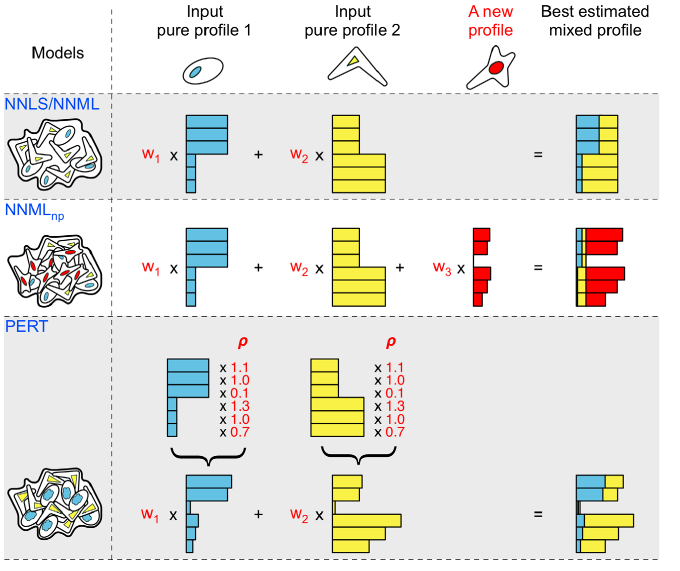
\includegraphics{figures/pert_probalistic_model.PNG}
%\caption{The main four assumptions of the probalistic models benchmarked
%by PERT approach}
%\end{figure}

TEMT (Transcript Estimation from Mixed Tissue samples)
\autocite{li_xie13} is also a
probabilistic model used for deconvolving mixture samples, originally
designed to infer the proportion of transcripts from a two-component
mixture (for instance, setting apart tumoral and normal immune cells)
but that can easily extended to deconvolve any number of cell
populations, provided a purified expression profile is available.
Instead of the \acrshort{RNA-Seq} counts generally required for most of the
deconvolution analyses (an integer number for each sampled transcript),
the read sequence is required, as well as length and sequence of the
transcripts. Actually, one read can be asserted to multiple transcripts
due to alternative splicing (a single DNA coding sequence for a gene can
produce distinct mature RNA transcripts, encoding possibly for proteins
with various functions) or similarity of the sequence, with a higher
proximity among homologous genes. One of the main objective of TEMT,
making it applicable for normalization of purified samples, is removing
non-biological variability. Indeed, only a part of the differences
observed in the number of counts between the transcripts is explained
biologically (the nature of the cells sampled, for instance, Lymphocytes
B express more IL4R than the other cell populations, or the phenotypical
status), but another part is associated to technical artefact.
Accordingly, for two genes expressed in the same proportions in a given
cell type, the resulting transcript with the longer sequence (referred
as the \emph{effective length} in the paper) offers more priming sites
to the RNApolymerase to start the transcription, and accordingly the
number of counts associated to it will be artificially superior. Even
trickier, the sequence itself can induce bias, resulting from both
\emph{positional bias} (starting positions of the processed reads are
not uniformly distributed along the sequence, but preferentially
distributed around the ends of the target transcript) computed before
using a binning method and \emph{sequence-specific bias} (the series of
nucleotides in the ends of the sequence, namely the proportions of A, C,
G and T nucleotides), estimated using Markov Chain. To our knowledge,
this is the only partial-based deconvolution method that directly
accounts for technical artefacts in their deconvolving process, as other
methods generally consider that input data has already been normalized
for such technical noise (TPM roughly corrects the effective length
bias, but doesn't deal with more specific sequence bias). Finally, the
last perturbation variable comes from the unknown cell population, which
is modelled similarly as in \(\text{NNML}_\text{np}\) algorithm (both
determination of its expression profile and its ratio). Instead of a
Dirichlet prior on the initial distribution of the ratios, a Gamma prior
has been used to initialize individually each ratio. The MLE of the
corresponding log-likelihood of the model is not analytically
computable, hence an online EM algorithm, whose convergence to the true
estimate was shown theoretically in
\autocite{dempster_etal77}, is used to retrieve an unbiased estimate of both the proportions
of a given transcript produced in a cell type, removing the technical
artefact, and the proportions of the cell type itself.
The DAGs describing the generative process of these probabilistic-based deconvolution models are represented in \Cref{fig:probalistic-model}

\begin{figure}
\centering
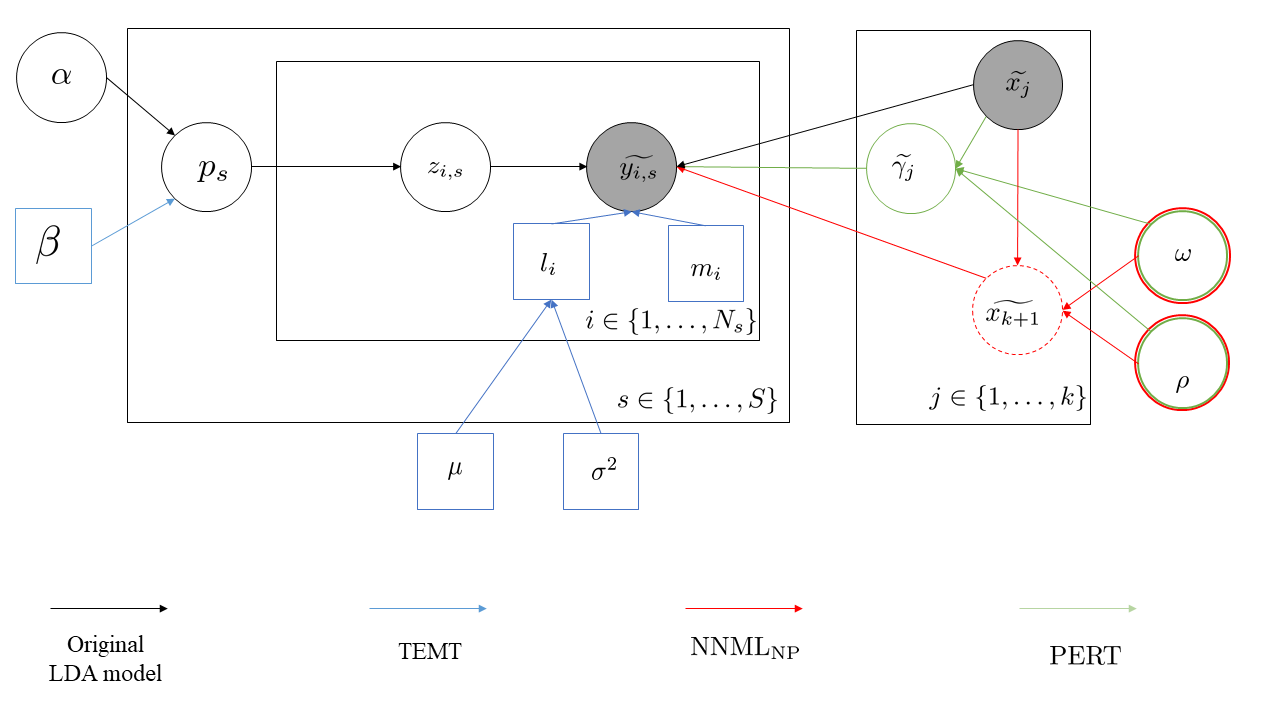
\includegraphics[width=0.5\textwidth]{figures/directed_probalistic_model.png}
\caption{The representative graphical models used to retrieve cell
ratios. More information on
\href{https://revbayes.github.io/tutorials/intro/graph_models.html\#legend}{legende
of a graphical model}}
\label{fig:probalistic-model}
\end{figure}

Lu and colleagues\autocite{lu_etal03} were the first to deconvolve cell proportions in the
transcriptome of yeast cultures in different phases of the cell cycle.
Wang and colleagues estimates immune cell populations (CD4+ and CD8+ T
cells, B and plasma cells and macrophages) in murine mammary gland
samples along with mammary epithelial cells and brown and white adipose
tissues. Following studies focus on the estimation of population cells'
proportions in blood samples, as the diversity of cell populations is
lower than solid tissues. Using transcriptomic profiles of purified cell
populations, these studies were able to estimate either the proportions
of lymphocytes, neutrophils and
monocytes\autocite{gong_etal11}, or 18
different immune cell populations \autocite{abbas_etal09}.


\subsubsection{Estimate cell-specific expression profiles}
\label{estimate-cell-specific-expression-profiles}

The usual method assumes that the gene expression of a cell subset is
uncorrelated to the remaining genes and independent of the
environmental. Hence, we can decompose the problem of retrieving the
cell-specific reference matrix for each gene, considering additionally
fixed expression per cell subset no matter the sample. Hence, the
individual gene expression for each sample is given by {[}{]}, where
this time, the cell specific expression profiles \(x_{ij}\) are the
parameters to estimate. Matricially, this yields for S samples the
following equality: \[
y_{i.}^T=x_{i.}^T \mathbf{P} , \quad y_{i.} \in \mathbb{R}^S, x_{i.} \in \mathbb{R}^{k}, \mathbf{P} \in \mathbb{R}^{k \times S}
\] and the LLS problem to solve is given by: \[
\hat{x_{i.}}_{\text{OLS}} = \arg \min_{\hat{x_{i.}}} \left( ||\hat{x_{i.}} \mathbf{P} - y_{i.}||^2 \right) = \sum_{s=1}^S \left( y_{is} - \sum_{j=1}^k p_{sj}\hat{x_{ij}} \right)
\]

As in CibersortX \autocite{newman_etal19} or the csSM algorithm in
\autocite{shen-orr_etal10}, it may
be possible to add a discrete explanatory variable for which in each
level the cell reference is fixed, but may vary from a condition to
another (for instance, sex or disease state). However, adding this
covariate implies, to keep a determined solution, that the number of
samples in each biological level is superior to the number of cell type
\(k\). Finally, instead of OLS, any linear regression method described
in the previous section can be used to solve the problem (yet, using
robust or SVR-based methods that include a filtering step, here on the
cell types selected, is not really relevant).

\[
x_{ij} \ge 0, \forall j \in \{1, \ldots, k\}
\] \[
Z_1, Z_2 \in \left\{1, \ldots, S \right\}, |Z_1| \ge 2, |Z_2| \ge 2, Z_1 \cap Z_2 =0
\]

\[
\begin{pmatrix}
y_{1, 1} & \ldots & y_{1, |Z_1|} & \ldots & y_{1, |Z_2|}\\
y_{2, 1} & \ldots & y_{2, |Z_1|} & \ldots & y_{1, |Z_2|}\\
y_{3,1} & \ldots & y_{3, |Z_1|} & \ldots & y_{1, |Z_2|}
\end{pmatrix}
=
\begin{pmatrix}
x_{1, 1} &  x_{1, 2}\\
x_{2,1} &  x_{2, 2} \\
x_{3,1} &  x_{3, 2}
\end{pmatrix}
\times
\begin{pmatrix}
p_{1, 1} & \ldots & p_{1,|Z_1|}\\
p_{2,1} & \ldots & p_{2,|Z_1|}
\end{pmatrix}
\]

\[
\forall i \in \left\{ 1, \ldots, 3 \right\}, \forall s \in Z_1
\] \[
y_{3, s} = a_1 y_{2, s} + a_2 y_{2, s}, \forall s \in Z_1, a_1, a_2 \in \mathbb{R}
\]


\subsection{Unsupervised and reference-free deconvolution methods}
\label{unsupervised-and-reference-free-deconvolution-methods}

Complete deconvolution algorithms attempt to simultaneously estimate
both the proportions and the pure expression profile of cell types
\autocite{shen-orr_gaujoux13},
without any additional information than the bulk profile. Such methods
are generally undetermined, thus they require prior information as well
as extra post-processing steps to assign the identified clusters to pure
cell types. Indeed, several optimal solutions can be found, and adding
prior information or constraint, can make the problem identifiable. They
are more sensitive to the amount and quality of data provided.

The first study proposing an algorithm to solve this problem was
published in 2001 by Venet and
colleagues\autocite{venet_etal01}. It
was an iterative method that estimates both \(\boldsymbol{X}\) and
\(\mathbf{P}\) by minimizing the absolute error,
\(|\mathbf{Y} - \boldsymbol{X} \times \mathbf{P}|\) that was applied to
deconvolve colon cancer samples. Interestingly, their method was able to
identify four cell populations, two of which could be identified as
hematopoietic cells and
fibroblasts\autocite{venet_etal01}.
The authors however discuss the limitations of their algorithm, notably
the selection of the appropriate \(k\) number of cell populations.

Repsilber and colleagues extended the method proposed by
\autocite{venet_etal01}, notably by
using a least-square non-negative matrix factorization algorithm,
alleviating one of the hypotheses necessary for the applicability of the
previously-proposed
model\autocite{repsilber_etal10}.
Erkkiläe implemented a Bayesian statistical framework that requires only
the number of distinct cell populations
\(k\)\autocite{erkkila_etal10}.

\autocite{wang_etal15} introduces
the UNDO R package that supplies an unsupervised deconvolution method to
impute both ratios and expression profiles specific to the tumour cells.
It requires however to identify marker genes (MGs) specific to the
tumour population studied. Previously,
\autocite{ahn_etal13} and
\autocite{quon_etal13} also address the
challenging task of purifying biological samples with immune infiltration and contamination in tumoral samples \footnote{Taking into account tumour heterogeneity in cancer genomics increases by several orders the sensitivity and specificity of DGEAs. Nevertheless, it is a challenging task due to the combination of an inter-tumour heterogeneity between different tumour types and an intratumour heterogeneity within a given sample (different tumour subclones). The current studies only addresses the inter-tumour heterogeneity, while in order to study intra-tumour
heterogeneity, either single-cell profiling data or sequences from multiple locations at different time points are needed.}.

Finally, UNDO \autocite{wang_etal15}
and CAM \autocite{wang_etal16} are
unsupervised approaches, allowing novel marker identification. To do so,
the expression matrix is projected in a K-dimensional \emph{polytope}
where each dimension \(K\) corresponds to a cell type present in the
mixture and the vertices to the associated marker genes. The R package
CAMTHC \autocite{chen19} implements the
completely unsupervised CAM algorithm with MDL visualization to help the
users selecting the right number of populations in their mixture. Prior
knowledge on some TMs for a cell type can increase the accuracy and
performance of the algorithm, in a semi-supervised approach where de
novo markers can be added by CAM algorithm. Both versions of this
algorithm are referred and benchmarked in
\autocite{jin_liu21} as CAMfree and
CAMmarker. Additionally, they provide a supervised approach to infer the
cell ratios with a LLS method when the pure signature is available and
NNLS independently for each gene when the cell ratios are provided.


\subsection{Marker-based approaches}
\label{subsec:marker-based-approaches}

In this type of approach, markers and expression profiles specific to a
cell type are required. Ideally, \emph{markers} are thought as genes
entirely specific to one population and robustly expressed in different
biological conditions. But to set apart highly correlated cell types,
this restrictive definition is often relaxed to a gene mostly expressed
in one cell type.

The markers investigated are sometimes proposed on immunology knowledge
Rooney et al. \autocite{rooney_etal15}, but are
most often based on empirical measures of purified (FACS-sorted or
in-vitro cultured) cell populations. The first approach to select marker
genes consisted in finding genes whose average expression value in one
cell type is greater than the expression value across the remaining cell
types \autocite{shoemaker_etal12}.
\autocite{chikina_etal15} extends this approach by assessing whether the difference was
statistically significant (combination of arbitrary fold-change and
\emph{p}-value approaches), by ranking markers based on SNR
(signal-to-noise) ratios \autocite{becht_etal16}, the F-statistic (testing whether adding an additional marker
is relevant in a multiple linear regression model)
\autocite{wang_etal10} or the Gini
index \autocite{zhang_etal17}.
Generally speaking, the methods used to discard genes belong to the
general machine-learning framework of \emph{filtering}, the
pre-processing step that removes irrelevant features before application
of a prediction algorithm
\autocite{guyon_elisseeff03}.

We now define theoretically the basis for using marker genes in
deconvolution problems. Let's consider a cell population \(j\), with
\(G_j \in \{1, \ldots, n\}\) the set of genes expressed uniquely in this
cell population. Then, for any gene from the marker set, we have the
following relation: \[
y_{i, i \in G_j}= \sum_{l=1}^k x_{i, l} \times p_{l} = x_{i, j} p_j, \text{ as } x_{i, l} =0, \forall l \neq j
\] where the existence of a mathematical solution in absence of noise
requires colinearity between the expression of the genes of cell
population \(j\) and the sample's expression of the corresponding genes
in the transcriptome \(y_{i, i \in G_j}\). This implies that for any
gene belonging to the market set, we have the following relationship: \[
p_{j}=\frac{y_i}{x_{i, j}}, \quad \forall i \in {G_j}
\] or, alternatively, that any gene expression is correlated to the
remaining genes of the market set.

This relationship can be generalized to \(S\) samples and to the \(k\)
cell populations of interest, with the genes expressed in the population
cells represented by the following \emph{block diagonal matrix} \[
\begin{pmatrix}
y_{G_1, 1} & \ldots & y_{G_1, S}\\
y_{G_2, 1} & \ldots & y_{G_2, S}\\
\vdots & \ddots & \vdots \\
y_{G_nn,1} & \ldots & y_{G_n, S}
\end{pmatrix}
=
\begin{pmatrix}
x_{G_1, 1}  &\ldots & 0\\
0 & x_{G_2, 2}   & 0\\
\vdots & \ddots & \vdots\\
0 & \ldots & x_{G_k, k}
\end{pmatrix}
\times
\begin{pmatrix}
p_{1, 1} & \ldots & p_{1, S}\\
p_{2, 1} & \ldots & p_{2, S}\\
\vdots & \ddots & \vdots \\
p_{k,1} & \ldots & p_{k, S}
\end{pmatrix}
\] with \(x_{G_j, j}\) the expression of markers genes uniquely
expressed in population \(j\). We generally set apart unsupervised
methods where neither the reference signature nor the cell ratios are
provided from supervised methods where one of these elements is known.
But both methods assume that markers specifically associated to a cell
population exist. Furthermore, there's no deconvolution technics going
down to the transcript level, while alternative transcript expression
may help in setting apart close cell types.


%\subsubsection{Infer ratios}
%\label{infer-ratios}
%
%However, in real datasets, the linear relationship assumption is broken
%by the presence of a random noise:
%\(y_{j}=x_{j}\times p_{j} + \epsilon_j, \quad \forall j \in G_j\).
%Historically, marker-based deconvolution methods rely on the
%identification of one \emph{strong} marker with a gene expression
%specific to only one cell population Clarke, Seo, and Clarke
%\autocite{clarke_etal10}. \autocite{gosink_etal07} assumed that the minimal expression ratio between the
%mixture and the reference signature \(\frac{y_{j}}{x_{j}}\) can be used
%as a proxy, up to a multiplicative constant, of the population
%associated to gene \(j\). It was originally designed to estimate the
%tumoral proportion in heterogeneous samples, and may not well-adjusted
%when retrieving ratios of several cell types. Additionally, it assumes
%that the noise effect is minimal and that a gene is uniquely expressed
%in the population of interest. An extension of this work is proposed in
%\autocite{clarke_etal10}
%that use the same algorithm but applies a specific log transformation.
%This may reduce the noise impact associated to small ratio values and a
%general underestimation of the true proportion. However, as suggested in
%several benchmarks Fa et al. \autocite{fa_etal20},
%log-transformation generally has a negative impact on the performance.
%
%More recent studies alleviate the null-expression condition, identifying
%\emph{weak} markers over-expressed in a given cell population but with
%possibly non-null expression levels in the others. They also focus on
%identifying not only one specific gene per cell type, but a collection
%of them, which is then either aggregated into an abundance score
%(MCPcounter, Becht et al., 2016) or an enrichment score (xCell, Aran et
%al., 2017).
%
%The abundance score is computed by averaging the expression ratios of
%the bulk mixture and the reference profile over the set of markers Becht
%et al. \autocite{becht_etal16}, and may be used as
%an approximate estimate of the ratios of cell subsets:
%
%\[
%\hat{p_{j}}=\sum_{i=1}^{n} \frac{y_i}{x_{i, j} |G_j|} \mathbb{1}_{i \in {G_j}}
%\] with \(|G_j|\) the number of marker genes associated to population
%\(j\). In doing so, we compute a more robust abundance score to the
%previous methods taking into account only one marker Clarke, Seo, and
%Clarke \autocite{clarke_etal10}, as the presence of
%an aberrant transcriptomic profile among the set of markers genes may be
%alleviated by the remaining genes. Both methods differ on the filtering
%of cell populations investigated and on the selection of marker genes.
%In \autocite{angelova_etal15}, a
%first cutoff of two FC is applied for the selection of candidate genes
%and then refined by considering only genes highly correlated to each
%other within a marker set. GSEA is then used to identify cell
%populations truly present in the mixture, keeping those enriched in the
%patient sample. In \autocite{becht_etal16}, the selection of TM relies on a compendium of 3 filters: AUC,
%fold change and a tailored fold change that preferentially selects genes
%both highly specific to a cell population and little variable in the
%remaining cell populations. Alternatively to the average of ratios
%proposed above, they propose the MCP-counter score, which is simply the
%log of the geometric mean of the bulk expression of the
%TMs:\(p_{k0} \propto \left(\prod_{j=1}^{n_{k_0}} y_j\right)^{1/k_0}\).
%This score is supposed to be correlated with the true ratio of the
%investigated cell population.
%
%Most of the methods computing an enrichment score (ES) rely on a
%weighted version of the ssGSEA (single-sample gene set enrichment
%analysis) principle, developed first by
%\autocite{subramanian_etal05}
%and \autocite{barbie_etal09} to
%determine whether a gene set was differentially expressed in a given
%biological sample. Let's consider a set of marker candidates for a given
%population \(k_0\) and rank the total number of genes \(n\) of the bulk
%mixture by their normalized expression level (or any other measure of
%the magnitude of their expression). The ES of the marker genes is given
%by: \[
%ES (y_{n_{k_0}}, \overline{y_{n_{k_0}}})=\sup_{i=1}^n \left| P_{y_{n_{k_0}}}(y_i) - P_{\overline{y_{n_{k_0}}}}(y_i) \right|
%\] where
%\(P_{y_{n_{k_0}}}=\sum_{j \le i}^{n_{k_0}} \frac{y_j^{\alpha}}{n_{k_0}}\)
%is the ECDF (empirical cumulative distribution function) of the marker
%genes, possibly weighted by an exponential term, and
%\(P_{\overline{y_{n_{k_0}}}} = \sum_{j \le i}^{n - n_{k_0}} \frac{1}{n - n_{k_0}}\)
%is the ECDF of the ranking of the remaining genes (remember that a
%marker gene is uniquely assigned to a cell population). When
%\(\alpha=0\), this is equivalent to the standard Kolmogorov--Smirnov
%statistic to compare empirical distributions
%\textcolor{red}{cucconi test might be relevant as well}. In all the
%reviewed papers that use this score, the ES was computed with the R
%\emph{gsva} function.
%
%In \autocite{bolen_etal11}, SPEC (Subset Prediction from Enrichment Correlation) is a
%two-step algorithm, aiming at linking a change in the gene expression
%with a specific cell population. To do so, enrichment scores (ES) are used as proxys of cell ratios
%for each sample, then the signature input provided by the user is associated to the cell lineage
%with the highest Pearson correlation in terms of ES. SPEC determines
%that the origin of the resistance to the standard treatment of HCV
%patients was the interaction between the myeloid cells and the
%anti-interferon therapy. In
%\autocite{rooney_etal15}, genes with
%at least 2-fold change greater than any observed in remaining cell types
%were selected as TMs. The goal of the study was to link the
%transcriptomic tumoral activity with the cell ratios observed in order
%to uncover mechanisms related to immune tumour resistance.
%\autocite{yoshihara_etal13}
%generates an immune and stromal enrichment score in a tumoral sample,
%averaging them into the E\acrshort{st}IMATE metric. It then uses the Eureqa
%software to determine the best link function associating the tumoral
%purity (proportion of tumoral cells in the sample) to the E\acrshort{st}IMATE
%score. The formula, fitted with the \emph{nls} function from the stats
%package is given by: \[
%\text{tumour purity} = \cos \left(a + b \times \text{E\acrshort{st}IMATE}\right)
%\] An extension of this method, combining metrics from alternative omics
%data, is proposed in \autocite{aran_etal15} paper. It's simply the average of the tumour purity
%estimations from four sources: the E\acrshort{st}IMATE score described above,
%ABSOLUTE (quantify the proportion of cancer cells based on the number
%and location of somatic copy-number mutations), LUMP (correlation
%between the degree of methylation and the tumour proportion) and
%immunehistochemistry image analysis (tumoral cells can be identified
%with specific fluorescent markers). In
%\autocite{senbabaoglu_etal16},
%gene signatures were obtained from biological knowledge, discriminating
%24 distinct cell populations in 19 cancer types. It was shown that
%over-expression of some cell types improved survival (Th17, CD8+ and
%Treg), while Th2 cells increase is associated to a negative prognostic.
%More recently, using a newly designed gene signature
%\autocite{aran_etal17}, xCell
%algorithm claims that it's able to identify up to 64 distinct immune and
%stromal cell types \textcolor{blue}{definition of a stromal cell}, using
%a compendium of 1822 pure human transcriptome. Additionally to a FC
%criterion, oncogenes were pre-filtered in the design of the reference
%matrix, and several signatures could be associated to a given cell type.
%To keep the linear relationship between the computed ES and the true
%cell ratio across several data sources, calibration was performed by
%means of a power function (only adjusted for average abundant cell
%ratios). Finally, the spillover effect that induces systemic bias in the
%ratios' estimation of highly correlated cell populations is
%counterbalanced by reducing correlated terms of the covariance matrix
%between the cell ratios.
%Finally, TIminer \autocite{tappeiner_etal17} is a freely Docker analytical pipeline. It uses the reference
%matrices provided by\autocite{aran_etal17}, \autocite{angelova_etal15} or
%\autocite{charoentong_etal17} to estimate the enrichment of tumour immune cell types, along
%with neoantigen prediction and tumour immunogenicity to characterize the
%tumoral environment.
%
%\autocite{shoemaker_etal12}
%propose the CTen (cell type enrichment) web-based tool able to
%automatically retrieve highly specific cell's gene expression in
%user-provided pure cell population transcriptome. Enrichment score in
%that paper is the negative log10 of the \emph{p}-value of a a Fisher's
%exact test. A significant \emph{p}-value rejects the null hypothesis of
%independence between the over-expression status of a gene and its
%belonging to a specific cell type TM. In case of independence, we expect
%in average that the proportion of over-expressed genes within the marker
%set and the non-specific genes is equal. This method is not applicable
%when a large number of cell populations are considered or when the set
%of TM is too small. Additionally,
%\autocite{abatangelo_etal09}
%shows that the Fisher's exact test is much worse in detecting small
%enrichments. Another alternative is proposed by the Bioconductor package
%BioQC \autocite{zhang_etal17}, where
%the enrichment of a marker set is asserted comparing the median
%expression of the TMs with the median expression of the bulk mixture,
%asserted with the non-parametric \emph{Wilcoxon-Mann-Whitney test}.
%
%Last but not least, both abundance and enrichment methods do not return
%the exact relative proportions of cell populations in the bulk sample,
%but only a score correlated to it. While most studies assume that
%there's a linear relationship between the score and the true ratio,
%\autocite{aran_etal17} is the
%only marker-based method in our review that attempts with numerical
%simulations to clearly retrieve the parameters of a link function, which
%reveals non linear (here, a power function). Hence, as opposed to whole
%transcriptome based methods, marker-based technics are more dedicated to
%inter-sample comparisons than intra-sample comparison.
%
%
%\subsubsection{Infer reference profiles}
%\label{infer-reference-profiles}
%
%\autocite{kuhn_etal11} and \autocite{kuhn_etal12} design the
%Population-Specific Expression Analysis (PSEA), the only method of our
%review using FACS data to estimate cell type-specific expression levels.
%Their method includes an intersection term to include non accounted cell
%types in the bulk expression, however they assume that within a
%biological group, the specific expression of a given cell type is the
%same for all individuals. It has been designed to identify the
%correlation between expression changes in astrocytes and Alzheimer's
%disease progression. More generally, their design is more adjusted to
%perform differential analyses testing whether the specific expression of
%a gene within a cell type is differentially expressed in relation with a
%biological condition. \autocite{reinartz_etal16} paper supplies as well a method dedicated to infer cell
%type specific expression, but it requires pure reference signatures of
%the cell types of interest, with small overlap between their
%transcriptomic expression. Additionally, the cell ratios and corrected
%pure cell types expression in a mixture are systematically biased, with
%an underestimation of the infiltrate cell type, or even worse, the
%adjustment performed is likely to be confounded with the natural
%variability of the transcriptomic expression.
%
%\todo{look at EPICabsolute and TIMERtumor}
%
%
%\subsubsection{Infer ratios and pure transcriptomic expression}
\label{infer-ratios-and-pure-transcriptomic-expression}

One of the first unsupervised technics, requiring only a set of specific
TM for a given cell type, is the Digital Sorting Algorithm (DSA) Zhong
et al. \autocite{zhong_etal13}{]}. First, we
hypothesise that the pure expression of a TM can be summed up by its
mean, yielding the following pure reference matrix:

\begin{equation}
\widetilde{\boldsymbol{X}_{1:k, 1:k}}
=
\begin{pmatrix}
\overline{x_{n_1, 1}}  &\ldots & 0\\
0 & \overline{x_{n_2, 2}}   & 0\\
\vdots & \ddots & \vdots\\
0 & \ldots & \overline{x_{n_k, k}}
\end{pmatrix}
\label{eq:marker-based}
\end{equation}

where \(\overline{x_{n_j, j}}\) is the average expression of the TM
set of population \(j\). Then, using \Cref{eq:marker-based} and simplex-unit constraint, listed in \Cref{eq:simplex-constraint}, we obtained the
following system of linear equations, with \(k\) unknown pure aggregated
TMs: \[
\begin{cases}
\sum_{j=1}^k \frac{y_j1}{\overline{x_{n_j, j}}}&=1\\
& \vdots \\
\sum_{j=1}^k \frac{y_jS}{\overline{x_{n_j, j}}}&=1
\end{cases}
\] Provided that the number of samples exceeds the number of cell types
(\(k < S\)), we can solve the system, and use the corresponding
aggregated matrix \(\widetilde{\boldsymbol{X}_{1:k, 1:k}}\) to retrieve the cell type ratio matrix with
classic linear regression. Once done, the estimated cell ratios are used
to retrieve the distinct pure expression profile, using
quadratic programming with bounded constraint for the expression.
CellCODE \autocite{chikina_etal15} models the proportion of the cell type of interest as a
surrogate variable, retrieved as the first right singular vector
(denoted as \emph{eigengene}, contributing the most to the variability
observed in the considered TM set). To reduce the searching space, the
estimation of the surrogate proportion variable (SPV) is restrained to
an user set of TMs specific to the cell population of interest.
Additionally, to account for the biological effect, it's possible to
integrate the design experiment in the study, although limited to a
single explanatory variable. The main purpose of this study is then to
integrate the estimated ratios to demingle the effect resulting truly
from a dysregulated expression of the TM to the effect of a modification
in the cell population. Their study notably shows that using this
process increases the sensitivity of their differential analyses.
However, we should note that the additional variability captured by the
surrogate variable may not be explained by a change in cell population
composition but rather from a technical effect or an uncaptured
biological condition \autocite{venet_etal01}.




\subsection{Alternative omic data types used for the deconvolution}
\label{alternative-omic-data-types-used-for-the-deconvolution}

Recently, epigenomics has been increasingly used for the deconvolution
problem. EpiDISH
\autocite{teschendorff_etal17} and methyICC \autocite{hicks_irizarry19} infers cell-type composition using DNA methylation data
and a reference profile of the CpG sites. Indeed, the degree of
methylation of the CpG sites of the DNA sequence is highly correlated to
the level of the gene expression and highly specific for a given gene to
the cell population. TOA\acrshort{st} \autocite{li_etal19}, BayesCCE \autocite{rahmani_etal18}, Edec \autocite{onuchic_etal16}, RefFreeEwas
\autocite{houseman_etal16} and MeDeCom \autocite{lutsik_etal17}
retrieve both the cell ratios and methylome reference profiles in a
completely unsupervised manner. Most of these methods use the same NNMF
algorithm, but set apart in the details of the implementation of the
method. For instance, RefFreeEwas initiates the population clusters
using hierarchical clustering, while Edec and Medecom use random
initialisation. Finally, Aran et al.~(2015) built a score, the Consensus
measurement of Purity Estimation, to evaluate the tumour purity in the
sample, combining transcriptomic, somatic copy number, methylation and
immunohistochemistry data.

However, as Teschendorff and Zheng (2017) pointed out, there's currently
no benchmark comparing the cell ratios retrieved from either
expression-based or DNA methylation-based, neither any attempt of
multi-omic integration data to solve the deconvolution problem.


\section{Feature selection}
\label{sec:feature-selection}

\todo{to be linked with the RNA-Seq pipeline}

Generally, following steps are considered for solving bulk mixture problem:

\begin{itemize}

\item
  creation of a reference gene signature profile when not provided
\item
  mixture model solved using svr or linear regression
\item
  statistic tests evaluating for each cell ratio estimation if it's
  significantly different from 0
\item
  (if provided) comparison with reference cell ratio measures, for
  instance using flow cytometry for instance
\end{itemize}

\todo{un-normalized RNA-seq is more accurately described by a negative binomial distribution// methods that do not rely on data normality, like LDA models, cf finotello in review section.}

The definition of a \emph{transcriptomic marker} for a cell population
is unclear and varies from one study to the other. In most partial
deconvolution approaches, the used markers of cell populations are
simply the differentially expressed genes.

Cell-types matrices were obtained by differential expression analysis.
Differentiation is asserted via an unequal two-sided variance t-test,
and a global \(q-value\) is computed (FDR process, with an extra step of
estimation of \(H_0\) distribution of p-values). For the estimation of
the total number of distinct genes to be used \(n\), \emph{condition
number} was applied to assert stability and robustness of cell
signatures with noise (especially presence of other cell types or
specifific phenotypic conditions), keeping the one with the lowest
condition number obtained with \(n=547\). With CIBERSORT, such a process
is done using \emph{kappa} function.

To derive a signature from that matrix, an extra-step of filtering is
required, to remove irrelevant feature (in our case, remove genes that
are not useful to discriminate several cell types). This enables a
faster computation (removal of genes with uniform expression, no matter
the cell type, such as those implied in metabolic processes) and a
greater signal-to-noise ratio, by keeping the most discriminatory genes
in terms of expression.

For LM22, either RMA or MAS5 normalization was performed, with HUGO
annotation, for Affymetrix chips. Illumina BeadChip was analyzed using
background correction of limma package \emph{normexp}. All microarray
studies were also processed a quantile normalization step.

An extra-step specific to LM22 generation consisting in a two-step
filtering was performed:

\begin{itemize}
\item
  Exclude genes presenting a too-much enriched expression in
  non-hematopoietic cell types. To that purpose, using enrichment scores
  from Gene enrichment profiler, they exclude all genes whose expression
  score was found higher at a threshold of \(5\%\) in non-hematopoietic
  cells or tissues (that's say not linked with blood cells or blood cell
  formation). We thus remove the ones not specific to the cell types we
  want to describe.
\item
  Second step is removing all genes with a heavy expression (superior in
  log scale to 7) in cell lines profiled in CCLE.
\end{itemize}


Ultimately, although \acrfull{scrna} (see \Cref{subsec:sc-rnaseq}) and \acrfull{st} (see \Cref{subsec:st}) had revolutionised the transcriptomics, we anticipate continuous uphold for the integration of deconvolution techniques as a complementary tool, since both methods are far from reaching the sensitivity and affordability of more traditional \acrshort{ngs} methods. Integration of deconvolution methods enhance the precision and robustness of downstream analysis, notably for identifying in a holistic framework key drivers involved in cell type-specific differential gene expression.


\section{Useful links: Benchmark of deconvolution methods in scientific literature}

Several benchmarks have been developed recently to compare the
performances of numerical deconvolution methods in relation with the
cell type sampled (presence of unknown or highly correlated cell types,
rare populations poorly represented in the transcriptomic compendium, )
(\autocite{sturm_etal19}), the
pre-processing protocol before applying the deconvolution algorithm
itself (\autocite{fa_etal20}) or the
quality of the mixture sample itself (noise structure and magnitude,
number of cell populations to identify, presence of unknown cell types)
\autocite{jin_liu21}.

\begin{enumerate}
\def\labelenumi{\arabic{enumi}.}

\item
  \autocite{fa_etal20} benchmarks several
  combinations of scaling/normalization and transformation technics with
  deconvolution algorithms. \emph{Data normalization} covers all
  techniques to make samples' distribution comparable, including various
  scaling methods (min-max, \emph{z}-score, row or column-wise) and
  methods dedicated to a specific technology, such as \emph{TPM} or
  \emph{FPKM} with RNA data. They may also correct technical artefacts,
  for instance, in \acrshort{RNA-Seq} data, lowly expressed genes are associated
  with a higher variability. The library size (the total number of
  counts measured in a given sample) may also differ between the
  samples. Data scaling approaches transform the data into bounded
  intervals. \emph{Data transformation} refers to the \emph{link
  function} applied on data, such that the assumptions on the
  distribution apply. \emph{Linear transformation} is simply the
  identity link function, with no transformation of the data. Another
  common transformation in transcriptomics data, especially for
  \emph{DGEA} analyses, is the \emph{log2} transformation to make the
  transcripts distribution Gaussian. All pre-processing methods and
  algorithms used to retrieve cell ratios in
  \autocite{fa_etal20} benchmark are
  summed up in the following picture:
\end{enumerate}

\begin{figure}
\centering
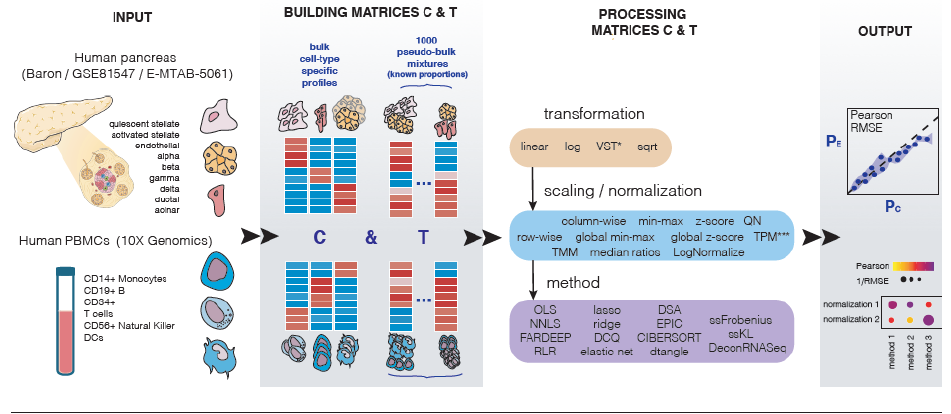
\includegraphics[width=0.9\textwidth]{figures/benchmark_GEP_schema.PNG}
\caption{Benchmark GEP technics}
\end{figure}

Both measures, independently on the platform (\acrshort{RNA-Seq} or microarray) used
or the tissue sampled, concludes that the log-normalization is
underachieving, with best results yield without any data transformation.
\emph{Scaling}, by smoothing extreme values, decreases the overall
performance, while \emph{normalization} within samples, for instance
batch correction of a technical artefact, have little impact on the
results (at the exception of row scaling, column min-max, column z-score
or quantile normalization that yield sub-optimal performances).
Specifically, Jin and Liu \autocite{jin_liu21}
shows that the best performances were reached when both the reference
signature and the bulk matrix of the measured transcripts were applied
the same normalization protocol. Specifically, quantification unit
technics (CPM, TPM, \ldots) that normalize \acrshort{RNA-Seq} data by library sizes,
with TPM being the most commonly used technics, present the best
performances overall.

Pre-filtering genes having the best discriminating power (ones with the
highest expression difference within cell type) tends to improve the
results. More precisely, the highest reproducibility of deconvolution
methods is reached by optimizing the \emph{condition number} (CN) of the
designed reference profile (A. Newman et al.
\autocite{newman_etal15}). Benchmarks on real
datasets seem to show that it was minimal with a moderate number of
genes selected. The CN is given by the following equation,
\(||\boldsymbol{X}|| \times ||\boldsymbol{X}^{-1}||\), with \(||\quad||\) the
Frobenius norm, and can be interpreted as an upper bound on the
precision of the obtained solution. With a CN of 1 (best case), the
accuracy of the solution is of the same order as the intrinsic
variability of the data. The lowest CN (1) is obtained for an orthogonal
matrix, implying in our deconvolution context that the transcriptomic
expression is independent between the cell populations.

The expression profiles are platform-specific, which might result in
markers not being captured by all platforms and in expression levels
depending on the choice of the platform. To counterbalance technical
artefact, CibersortX \autocite{newman_etal19} supplied a batch-correction effect using the Combat
method. Generally, Cibersort, CibersortX and MuSiC are the least
impacted by the choice of normalization protocol. Additionally,
single-cell deconvolution methods in which the reference signature
proceeds explicitly from  \acrshort{scrna} data do not show significant
improvement over more classical methods based on bulk-deconvolution
methods.

\begin{enumerate}
\def\labelenumi{\arabic{enumi}.}
\setcounter{enumi}{2}

\item
  Most of the methods are highly sensitive to the absence of a cell
  population in the reference signature when it's really present in the
  bulk mixture. Hence, \autocite{sturm_etal19} concludes that the best estimates are reached when the
  reference profile is representative of the true bulk cell population.
  Interestingly, the highest deviations occur in absence of
  significantly correlated cell types (\emph{multicollinearity} refers
  to situations where more than two cell types are strongly correlated).
  For instance, the performance in terms of correlation and mean
  absolute deviation (mAD) is highly decreased when mDC (myeloid
  dentritic cells) are present in the mixture, due to their proximal
  expression with monocytes. Especially, when the proportion of a given
  cell population is higher than expected, occurring especially when
  related cell types are not referenced in the signature,
  \autocite{sturm_etal19} mentions it
  as \emph{spillover effects}. They tend to have a greater impact on
  marker-based approaches. \emph{Background prediction} tackles with the
  opposite problem, when a cell ratio is statistically different from zero while it was not present in the mixture. It may explain why most of the numerical deconvolution methods are
  biased, tending to over or underestimate most of the cell types in the
  sample. Additionally, marker methods require an enough number of distinct
  genes (5-10) to identify unequivocally a cell population
  \autocite{ahn_etal13}, especially to
  deal with possible outliers. This issue is exacerbated when some of
  the genes used in the reference signature are both expressed in
  low-abundance and more abundant cell subset (\emph{signal dilution
  effect} \autocite{shen-orr_gaujoux13}. More precisely, \autocite{fa_etal20} suggests that removing a cell type that is uncorrelated
  to all other cell types remaining in the reference matrix tends to
  biased estimates of the ratios of all other cell types while removing
  a cell type that is strongly positively correlated with cell types
  still present in the reference matrix leads to biased estimates
  specifically for them. CibersortX, Cibersort and MuSiC are the least
  sensitive algorithms to the presence of highly-correlated cell types
  or to the presence of rare cell types in the
  mixture\autocite{jin_liu21}
  Additionally, some rare cell types, some being recently discovered,
  may not have been profiled yet, leading to systematic bias in the
  estimation of the cell ratios. This is especially an acute problem
  with tumoral profiles due to the unique patterns of mutations and the
  possibility diversity of subclonal populations. Methods specifically
  tailored to deal with infiltration of cell populations of unknown
  transcriptomic expression, such as TIMERtumor
  \autocite{li_etal16} or EPICabsolute
  \autocite{racle_etal17}, present the
  least biased cell ratio estimations in presence of unknown tumoral
  content.
\end{enumerate}

The results are really dependent on the \emph{phenotypic and tropic
condition}, and the discrepancy between the phenotype (age, gender,
disease status\ldots) of the references samples and the samples in which
the deconvolution is performed could bias the estimated cell ratios.
Additionally, even with similar tissues, individual singularities such
as cellular \emph{heterotypic} contamination (for instance, infiltrates
of tumoral cells), disease-induced or microenvironment dysregulation can
significantly modify the native transcriptomic profiles of the cell
populations compared to healthy tissues. Finally, most reference
profiles provided by deconvolution methods lack samples to capture the
variability of intracellular expression. For instance, the mean
expression of some of the cell types in the LM22 signature of Cibersort
\autocite{newman_etal15} was
estimated from three distinct samples.

In order to get closer from the true biological dynamics, deconvolution
methods could integrate the dynamics of cells types, as in each sample,
different phases of the cell cycle, characterized by varying levels of
transcriptomics expression activity, coexist. While in cultured cells,
the cell cycle can be synchronized by chemical arrest or nutrient
starvation \autocite{bar-joseph_etal08}, this is not possible when alive tissue samples are profiled.

While most methods assume that the expression of individual markers is
independent of the population ratios, Kuhn et al.
\autocite{kuhn_etal11} show that \emph{paracrine}
(proximal cellular communication altering only the behaviour of
neighbouring cells) signalling effects induce high cross-product values
across transcripts.

\begin{enumerate}
\def\labelenumi{\arabic{enumi}.}
\setcounter{enumi}{3}

\item
  Penalized regression approaches including Lasso, ridge, elastic net
  regression and DCQ performed in average slightly worse compared to the
  other deconvolution methods. Quadratic programming (DeconRNASeq),
  Digital Sorting Algorithm (DSA) and the semi-supervised approaches
  ssKL and ssFrobenius (using only sets of marker genes, in contrast to
  the supervised counterparts which use a reference matrix with
  expression values for the markers) showed the poorest performances. As
  against, regression-based (least-squares, support-vector (CIBERSORT)
  and robust regression (RLR, FARDEEP) approaches) bulk deconvolution
  methods, coupled with single-cell data, have the best performances.
\end{enumerate}


%\section{Applications of numerical deconvolution methods}


\label{applications-of-numerical-deconvolution-methods}


\subsection{Differential analysis}
\label{differential-analysis}

\autocite{elloumi_etal11} is one of
the first authors highlighting the loss of power and the risk of wrongly
identifying transcripts expression as prognostic markers of a disease,
when the biological effect is confounded with a change in cell
composition. Indeed, it shows with numerical simulations that ignoring
the contamination of normal cells within tumour cells deflates the power
of detecting breast genomic predictors.

The algorithm \emph{contamDE} \autocite{shen_etal16} offers to model each gene expression in the tumoral
mixture as the contribution of pure tumoral and normal cell population
weighted by their proportion in the sample. The total number of counts
retrieved from \acrshort{RNA-Seq} experiment is hence modelled by the sum of two
negative binomials (NBs), a commonly used probability distribution in
such study. The specificity of their model is to integrate directly the
effect of cell proportion as well as the normalization factor (when the
depth sequence is heterogeneous along with the sample) in the negative
distribution: \[
Y_{ij}^{\text{pure}} \sim \text{NB} (\kappa_j \mu_i, \phi_i) \text{ and } Y_{ij}^{\text{mixture}} \sim \text{NB} (\kappa_j^{'} \left( \mu_i + \omega_j \delta_i\right) , \phi_i)
\] where \(Y_{ij}^{\text{pure}}\) is the number of reads of gene \(i\)
for the \(j^{th}\) sample, \(Y_{ij}^{\text{mixture}}\) the number of
reads in the mixture sample, accounting for both the contribution of
tumoral and normal cells, \(\kappa_j\) and \(\kappa_j^{'}\) are
normalization factors and \(\delta_i = \mu_i' - \mu_i\) the true mean
expression difference between tumours and normal cells. Relevant
prognostic markers are those for which this difference, \(\delta_i\), is
not null. It's worth noted that this distribution is different from the
following mixture model, 
\[
Y_{ij}^{\text{mixture}} \sim (1 - \omega_j) \text{NB} (\kappa_j \mu_i, \phi_i) + \omega_j \text{NB} (\kappa_j^{'} \left( \mu_i + \delta_i\right) , \phi_i)
\] 
that could be expected to simulate the two counts sources, the
purpose being to ease the difficulty of deriving confidence intervals of
DE genes. They also include another model in their analysis, adding an
additional fix effect, to account for possible correlation when the pure
sample and the mixture sample proceed from the same source. Finally, the
unknown parameters of the model (mean of the genes distribution and cell
proportion) are estimated with an iterative method and the final
\emph{p}-values are derived using a likelihood ratio test. However, to
make the problem identifiable, as the pure expression of tumoral cells
is unknown, an additional constraint on the ratios must be set, which
lead to systematic bias toward 1 between the estimated and the true fold
change (no bias in pure samples).

\todo{micro-environment application, \url{https://www.sciencedirect.com/science/article/pii/S0945053X23000811}}
%\section{Biological application}
%\subsection{Tumoral micro-environment}
%
%Cancer is one of the first causes of mortality in developed countries
%(first cause in France, second factor in the USA). In the meantime, it
%remains challenging to develop treatments adjusted to the wide diversity
%taken by cancer forms. Additionally, most of the existing treatments do
%not adjust to the specificity of the tumoral environment, and present
%numerous side-effects.
%
%However, recently, a newly developed treatment, cancer immunotherapy,
%using \emph{immune checkpoint blockers}, reveals highly successful in
%curing tumours that were resistant to standard drug therapies. But the
%tumour microenvironment (TME) {``Low-{Heterogeneity Melanomas Are More
%Immunogenic} and {Less Aggressive}''}
%\autocite{LowHeterogeneity19} is a complex network
%of an interwoven mixture of malignant cells and healthy cells, including
%immune cells and fibroblasts, that intercommunicate. And immunotherapy
%requires a comprehensive molecular and cellular characterization of the
%tumoral environment to elucidate the complex interactions intervening in
%the TME and develop therapies adjusted to any type of cancer form
%\autocite{finotello_trajanoski18}. Indeed, the mechanism of immuno-resistance remains largely
%unexplained, with cold tumours having a poor immunogenic activity with
%low infiltration of T cells and small response to immune checkpoint
%inhibitor therapy (as opposed to hot tumours).
%
%Next-generation sequencing (NGS) as well as novel technologies such as
%single-cell RNA sequencing ( \acrshort{scrna}) and mass cytometry by time of
%flight (CyTOF) provide large data sets that give relevant cues for the
%development of innovative treatments. Accordingly, storing, analysing
%and vizualizing the large and heterogeneous amount of data returned by
%NGS require an intensive research on developing adapted computational
%algorithms.
%
%The \emph{cancer-immunity cycle} \autocite{chen_mellman13}
%consists in the chronological description and evolution of the
%interactions between immune and tumour cells. Complete characterization
%of the tumoral landscape includes thus to retrieve information on
%neoantigens, immune contexture, the tumour microenvironment (TME), and
%global environmental factors.
%
%Cytotoxic CD8+ T cells are responsible for most of the anti-cancer
%response. First, it requires phagocytosis of a newly exogenous foreign
%protein, generated by the gene mutations or rearrangements occurring in
%tumoral cells, by an APC (antigen-presenting cell), generally a DC
%(dentritic cell). Then, proteolytic enzymes cleave the protein into
%smaller peptides that are transported to the cell surface via newly
%synthesized MHC class II molecules from the endoplasmic reticulum. Next,
%priming and activation of naive CD8 T cells occurs in lymph nodes where
%the antigen is presented by the MHC class II complex of an APC together
%with co-stimulatory signals. Finally, after clonal expansion and
%proliferation of the activated T cells, the anticancer immune response
%is exerted through recognition of an endogenous peptide bound to MHC
%(major histocompatibility complex) class I of tumoral cells (the
%so-called peptide-HLA complex) by the variable part of the TCR chain of
%a TCD8 cell and secretion of molecules such as granzyme B (GZMB) and
%interferon-\(\gamma\) (IFN\(\gamma\)) that lyse the cell membrane. It's
%worth noted that both MHC classes are encoded by distinct HLA gene
%complexes. Interestingly, the proteasomes of any cell type generate
%peptides from all proteins present within the cell that are presented to
%the surface, but their recognition as \emph{non-self} requires
%necessarily that the corresponding TCD8 \emph{clonotype} (populations of
%T cells that carry identical TCRs) has first been activated and
%amplified by an APC. Immune checkpoint blockers are monoclonal
%antibodies (specific to one antigen only) targeting receptors present on
%either tumour or immune cells that can boost the inflammatory response
%against cancer cells, generally by their antagonistic action on the
%inhibitory mechanisms developed by tumoral cells. The in silico
%prediction of the \emph{immunogenicity} (ability of a molecule to
%provoke an immune response) of neoantigens are at the core development
%of personalized cancer vaccination and immunotherapy. It requires three
%steps: first, identification of somatic mutations from paired tumour and
%normal tissue; second, genotyping of the patient's HLA genes and, third,
%prediction of peptides binding to the patient's HLA molecules. Two
%prognostic signs associated to a higher immunogenecity include the
%stability of the pHLA complex altogether with the \emph{avidity} (T
%cells with high functional avidity respond to low antigen amounts) of
%the TCR receptor, especially the CDR3 sequence, region of the variable
%chain that binds to the eiptope of the antigen Rasmussen et al.
%\autocite{rasmussen_etal16}, and the foreignness of
%the neoantigen \autocite{blank_etal16}
%(a never recognized peptide is more likely to induce a higher reaction).
%
%\begin{figure}
%\centering
%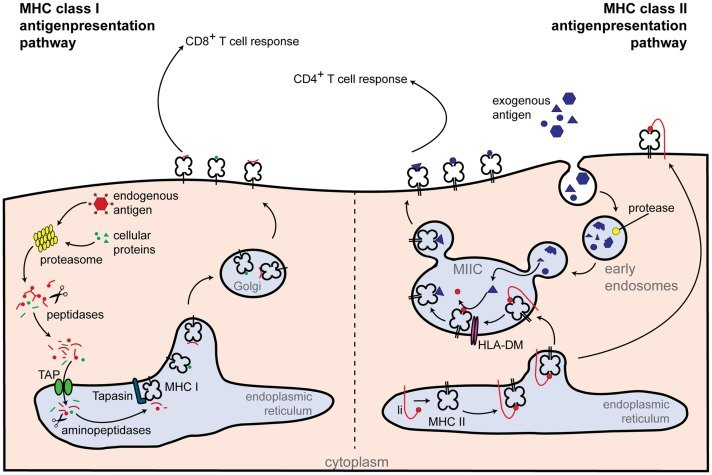
\includegraphics{figures/Classical-routes-of-antigen-presentation-by-MHC-class-I-and-II-molecules-Class-I-antigen.png}
%\caption{Description of the differences between the mechanisms of
%antigen presentation by- MHC class I and II molecules
%\autocite{neerincx_etal13}}
%\end{figure}
%
%The immune context describes the composition (ratio of effectors and
%suppressors cells of the immune reaction), the localisation of
%infiltrating (infiltrated: immune inflamed phenotype, confined at the
%tumour margins: the immune excluded phenotype or absent from the tumour
%mass: immune desert phenotype) and their state of activation. Indeed, by
%exerting pro- and anti-tumorigenic actions, tumour-infiltrating immune
%cells can profoundly influence tumour progression, as well as the
%success of anti-cancer therapies Galluzzi et al.
%\autocite{galluzzi_etal18}. For instance, cytotoxic
%CD8+ T cells can specifically recognize and kill tumour cells bearing
%neoantigens \autocite{chen_mellman13}, while regulatory T cells, by their immuno-suppressive
%functions, can enforce immune escape
%\autocite{finotello_trajanoski17}. Understanding the interaction and communication among distinct
%cell populations is also crucial to help understanding the evolution of
%the tumoral population. Proteomics and secretome (what is released into
%the extracellular space) data can help deciphering the various cell
%communication pathways, including chemokines or cytokines with their
%coupled receptor or immune checkpoint ligand--receptor pairs
%\autocite{rieckmann_etal17}.
%
%The spatial range of cytokine-mediated communication is also key to
%unveil the complex network of interactions between the cell populations,
%with three modes of cell signalling: \emph{autocrine signalling}, in
%which secreted cytokines are trapped by receptors from the same cell;
%paracrine signalling, in which secreted cytokines are trapped from
%receptors of cells belonging to the same tissue; and endocrine
%signalling, in which secreted cytokines are generally carried by blood
%vessels to distant remote tissues
%\autocite{thurley_etal15}. Analysing
%the ligand--receptor interactions helps recently to elucidate the
%mechanism of action of a ligand secreted by epithelial cell on a
%receptor present in cancer-associated fibroblasts of the ovarian cancer
%\autocite{yeung_etal19}.
%
%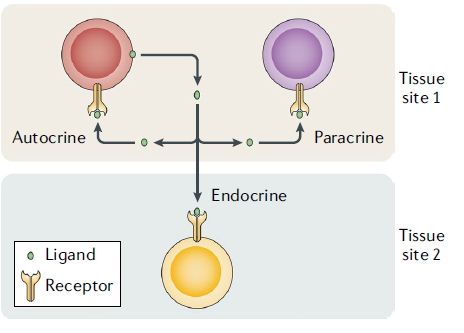
\includegraphics{figures/cell-cell_communication.PNG}
%
%The TME encompasses, in addition to tumoral and immune cells, other
%healthy non-immune cells, such as epithelial and endothelial cells,
%mesenchymal stem cells and cancer-associated fibroblasts (CAFs).
%Notably, CAFs release various tumour-promoting cytokines and chemokines,
%hence favouring tumour growth, angiogenesis (and so risk of the
%development of metastatis) and immunosuppression. Indirectly, pericytes
%play a role in the development of tumoral clones, by regulating the
%contracton of the blood vessels.
%
%Global environmental factors, such as angiogenesis, tumour-promoting
%inflammation and immunological competence of the patient, such as
%infection state or immuno-mediators drugs have a strong impact on the
%composition of the TME. Additionally, commensal microbes from the gut
%microbiota can modulate the antitumour immunity.
%
%
%
%Major challenges remain to understand this intricate system, including
%the comprehension of acquired resistance to immune checkpoint blockers
%therapy, the computational prediction of the strength of the
%immunological response, the identification of combined therapies with
%synergistic potential, the selection of neoantigens for therapeutic
%cancer vaccination and personalized therapy with tailored T cells
%targeting directly the identified clones.
%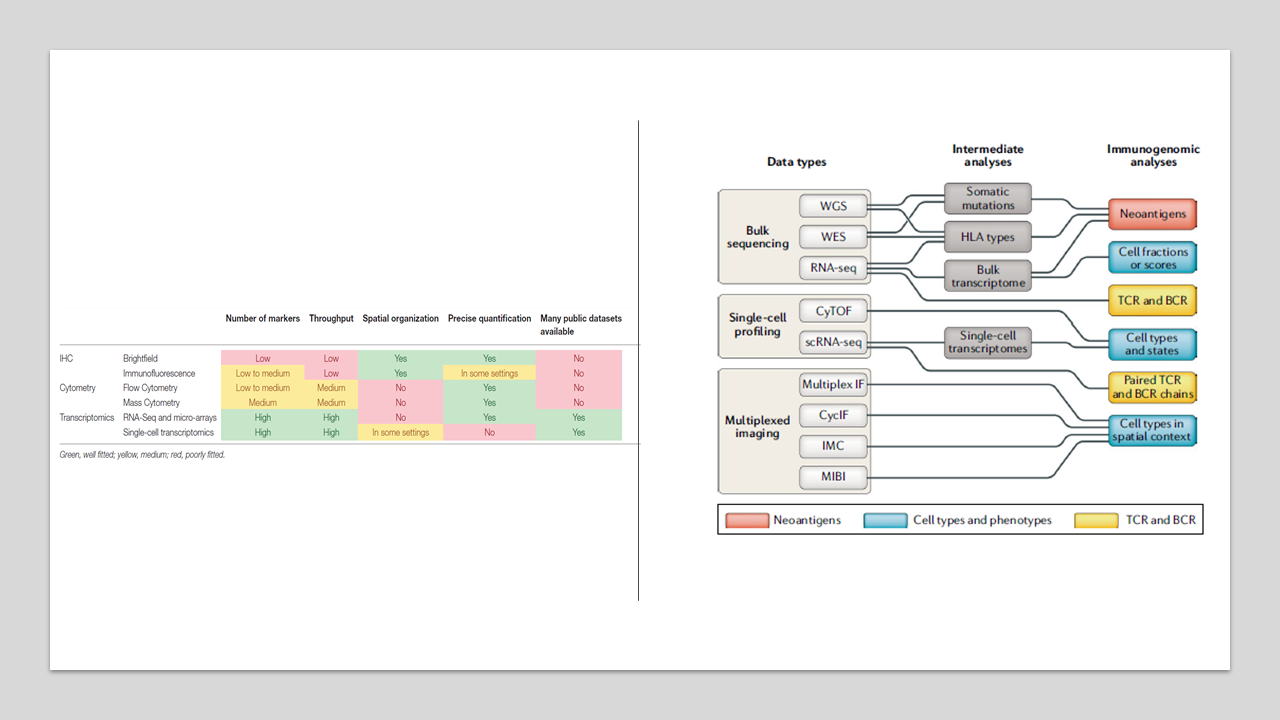
\includegraphics{figures/tme_estimation_technics.PNG} Finotello and
%Trajanoski \autocite{finotello_trajanoski18}








Several emerging promising methods aim at keeping the spatial
information of transcriptomic data along with the origin of identified
tumoral cell types. Using barcodes associated to different regions of
the analysed tissue prior to RNA-Seq, Ståhl et al.~and Salmen et
al.~pioneered the field of Spatial Transcriptomics
\autocite{salmen_etal18}. Recently, the
combination of contrast-enhanced tomography images with RNA-seq data
enabled to identify the radiomic signature of tumour-infiltrating CD8+ T
cells \autocite{sun_etal18}.
Simultaneous measures of distinct omics data, for example joint \acrshort{RNA-Seq}
and epitopes analyses (CITE-seq,
\autocite{stoeckius_etal17}), or
\acrshort{RNA-Seq} and proteomics data (REAP-seq,
\autocite{peterson_etal17}) could
unravel the tumoral cell signalling pathways. Indeed, dysfunctional
tumoral signalling arises from a combination of gene mutations with
epigenetic modifications, inducing rewiring of the signalling network \autocite{yaffe19}.
Additionally, regulation of cell signalling has a strong impact on the
fate of the tumoral clone, intervening in cell growth, cell-cell communications, cell cycle and cell death mechanisms. Last, most of
targeted drugs are directed against signalling molecules, combining them
would require computational predictive analyses of the pharmacological
signalling rewiring. Unfortunately, the crosstalk between oncogenic
signalling and signalling rewiring induced by drugs is still not used in
clinical decision-making due to the lack of reproducibility. And use of
RNA-seq data only as a surrogate of the protemics is suboptimal, as a
large part of the epigenetic regulation of signalling pathways is
performed at the post-transcriptional level. All these approaches could pave the way for non-invasive exploration of tumoral landscape and enable longitudinal monitoring of the effects of immunotherapy.

Alternatively, transferring information from one data set to another,using transfer learning approaches, is helpful to explore partial information. For instance, in study (181),  \acrshort{scrna} was used for cell
type annotation, enabling to reveal finer differences of gene expression
regulation processes spotted by chromatin accessibility data, generated
using sscATAC-seq technics. Last but not least, mathematical mechanistic
modelling provide quantitative predictions that can be experimentally
validated, with pioneered investigation on the dynamics of
tumorigenesis \autocite{iwami_etal12} or the development of Gemini in-silico patient models to predict the effects of combination therapies \autocite{kather_etal18}.




 \part{Mathematical Introduction}
 \chapter{Mixture models} 
\label{chap:gmm-benchmark}

\paragraph{Overview: variability in biological systems}

In general in absence of clear identified phenotype marker, it is common to assume the same generative model for patients belonging to a given cohort. 
However, we observe strong variability even between related samples, included within the same individuals. The variability may result from three distinct factors: at the environmental level (disease state, tissue location, \ldots), the genotypical level (presence of individual mutations inducing varying transcriptomic activity) and even at the cell population level. 

When unobserved, using a \textit{latent variable} to account for the intra-variability may reveal useful to discover unknown patterns. In the next section, we present one of the most commonly used statistic tool, namely \Glspl{gmm}, used to perform \textit{unsupervised} analysis. 


\section{Article 1: Gaussian Mixture Models in R}

\includepdf[pages=-]{gaussian_mixtures_benchmark.pdf}












 
\part{Biological Applications}

\leadchapter{Primary Sjögren's disease (pSD) is a complex and highly heterogeneous autoimmune disease, characterized notably by lymphoid infiltration of exocrine glands and autoantibody generation. The heterogeneity in clinical manifestations and pathophysiology of the disease make the current development of an effective treatment or an approved targeted therapy a highly intractable task. To address this issue, we conducted a large \emph{stratification study} on a \gls{cross-sectional} cohort of blood samples from 300 patients, with both molecular and clinical validation of Sjögren's syndrome, to identify well-characterised transcriptomic patient subgroups. These clusters were then further annotated with genomic, epigenetic, cytokine, autoantibody expression as well as flow cytometry and clinical data, as summarised in \Cref{fig:infographic-sjogren-clustering}.


Previous studies classified patients based only on their \acrshort{ifn} activation score status, yet, this study aims at extending these preliminary results, by adopting a comprehensive multi-omics approach. 


The clustering algorithm was performed on pre-processed RNAseq data, $\boldsymbol{Y} \in \mathcal{M}^+_{G \times N}$, with $G$ the number of genes not belonging to the background noise, and $N=304$ the final number of individuals selected under the protocol extensively described in \Cref{chap:transcriptome-workflow} and \Cref{subfig:rnaseq-sjogren-pipeline}

\begin{enumerate}
\item The top $25\%$ most variant genes, defined by their degree of 
variation coefficient(CV), were selected to perform the clustering analysis.

\item To determine the number of clusters, a robust clustering method, previously applied to breast cancer transcriptomic profiles, \autocite{guedj_etal12} and \Cref{subfig:consensus-clustering}, was performed:

\begin{itemize}
\item \emph{Agglomerative Hierarchical Clustering} (\texttt{hclust} function from R mclust package, \autocite{scrucca_etal16}), using Pearson correlation as a similarity measure 
\item $k$-means clustering \autocite{macqueen67}, using \texttt{kmeans} function from stats R package 
\item Gaussian mixture clustering (GMM) using \texttt{mclust function} from R mclust package \autocite{scrucca_etal16}.
\end{itemize}

\item Next follows a supervised analysis, performed on the 149 patients with consistent cluster assignments between the three clustering methods (considered as \enquote{core} groups) to retrieve the minimal transcriptomic signature to identify unambiguously the 4 clusters. A pre-candidate set of \num{3577} genes was selected from a classical one-way ANOVA
($\text{FDR} < \num {1.e-10}$), and then reduced by Random Forest to a final set of 257 top discriminating genes (\texttt{randomForest} function from randomForest \autocite{cutler_wiener22} R package). We then verified and confirmed afterwards the robustness of the clustering by re-applying Step 2 on our discovery set with the final minimal signature obtained.

\item Finally, patients inconsistently assigned with the 3 clustering methods were associated for each of them to their respective closest centroid, as measured by their correlation similarity score.
\end{enumerate}

Since this algorithm consists of iterated unsupervised and supervised steps, \autocite{guedj_etal12} classifies it as \enquote{semi-supervised} .


We eventually identified four distinct pSS patient clusters, illustrated in Heatmap \Cref{subfig:heatmap-sjogren}. Interestingly, they displayed distinct patterns of immune dysregulation, cellular composition and disease activities. Precisely, the four clusters were annotated as such:

\begin{itemize}
\item The C2 cluster displays a healthy-like profile, gathering patients with on average, lower disease activity and no \Gls{anti-ssa} antibodies.

\item  On the contrary, cluster C4 exhibited the strongest severe clinical phenotype signature, characterized by a prominent \gls{interferon} Type II activation signature, significant inflammation, massive \emph{lymphopenia} (unexpected decrease of lymphocytes) and monocytes decrease as well as higher levels of neutrophils, all tending to output an inflammatory phenotype. These observations were further corroborated by methylation analysis on \acrshort{dmp}, since they revealed that C4 had the highest number of hypomethylated genes related to IFN signalling, inflammation and neutrophils, knowing that high levels of gene expression are often associated with low promoter methylation \autocite{wagner_etal14}. Finally, we should note too that C4 is the less populated group, with only 38 patients ($12.5\%$) in it. Besides, 

\item The cluster C1 showcases the highest Type I and Type II \acrshort{ifn} scores, as exhibited by enrichment analysis studies of gene modules. Genome-wide association study (GWAS) analysis only pinpoint significant genetic differences in C1, particularly genes associated with the immune system, signal transduction and cell cycle.

\item While the cluster C3 is characterised by a strong Type I \acrshort{ifn} score. Additionally, C3 showed a significant activation of pathways related to B cell activation and higher levels of autoantibodies, further supporting the relevance of B cells as additional potential therapeutic targets for the patients assigned to this cluster.
\end{itemize}

We verified a posteriori that systemic treatments had no impact on the cluster distribution, since half of the pSS patients were undergoing antimalarial, immunosuppressive or steroid treatment. However, comprehensive sensitivity analyses showed that treatments did not significantly affect the distribution of patients within clusters.


We finally developed a composite model using machine learning approaches to predict to which cluster each patient belonged, using a reduced number of non transcriptomic variables. The accuracy of the model was high and validity confirmed using an external dataset of pSS patients as a validation marker. This model could help in selecting patients prior to clinical trials, more likely to display better therapeutic outcomes.
To conclude, we were able to provide a new patient classification into \emph{endotypes} (subgroup patients defined by distinct functional and metabolic mechanisms). 


\begin{figure}
     \centering
     \begin{subfigure}[p]{0.6\textwidth}
         \centering
         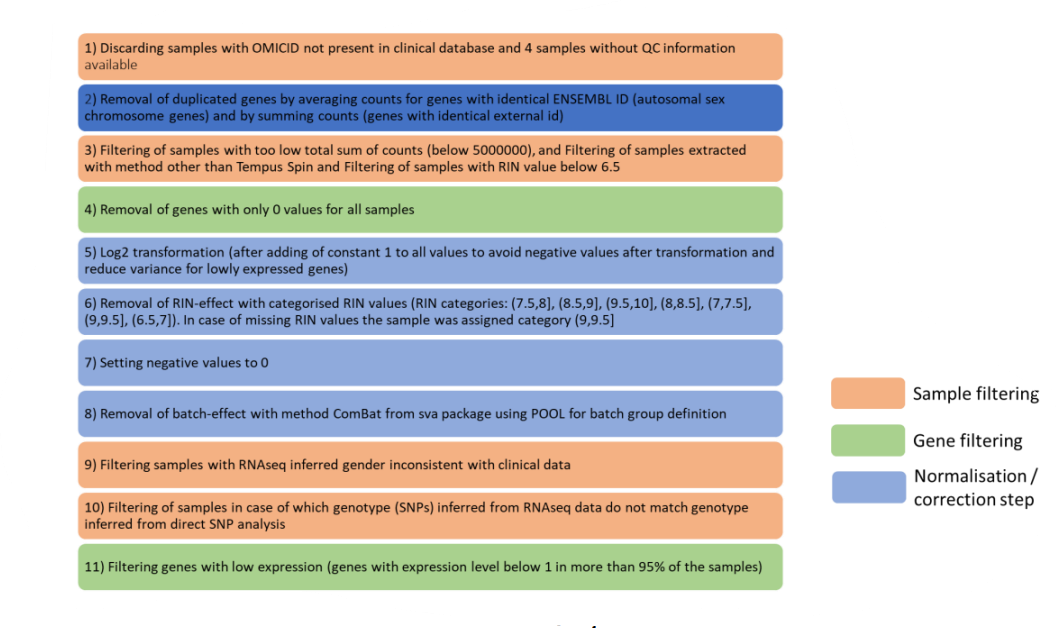
\includegraphics[width=\textwidth]{figures/sjogren/pre-processing.png}
         \caption[\textbf{RNAseq analysis flowchart}]{This flow-chart summarises the several steps used to pre-process and normalise RNASeq data. Notably, duplicated genes or displaying inconsistent updated HGNC gene annotations were discard. Log2 transformation and svt normalisation were then applied on gene expression data followed by removal of genes exhibiting low expression.}
         \label{subfig:rnaseq-sjogren-pipeline}
     \end{subfigure}
     \hfill
     \begin{subfigure}[p]{0.35\textwidth}
         \centering
         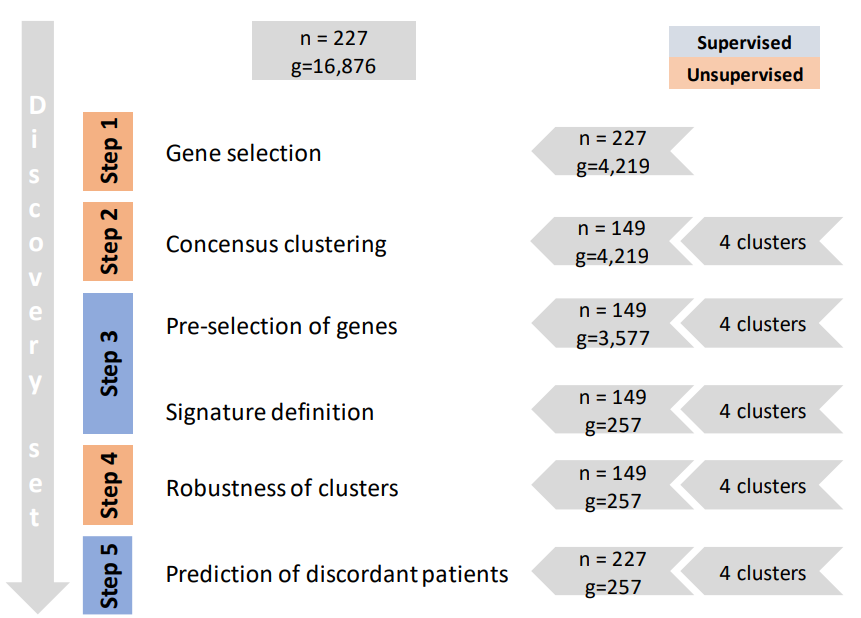
\includegraphics[width=\textwidth]{figures/sjogren/consensus_clustering.png}
         \caption[Flow chart of \enquote{semi-supervised} hierarchical clustering]{In brief, we classified Primary Sjögren’s syndrome (pSS) patients into 4 clusters using three comparable clustering algorithms. Out of the 227 patients, 149 yielded a consensus identification in each of the clusters, even after applying gene feature selection refinement, leading to a minimal reference signature of 257 genes. }
         \label{subfig:consensus-clustering}
     \end{subfigure}
     \vfill
     \begin{subfigure}[p]{0.6\textwidth}
         \centering
         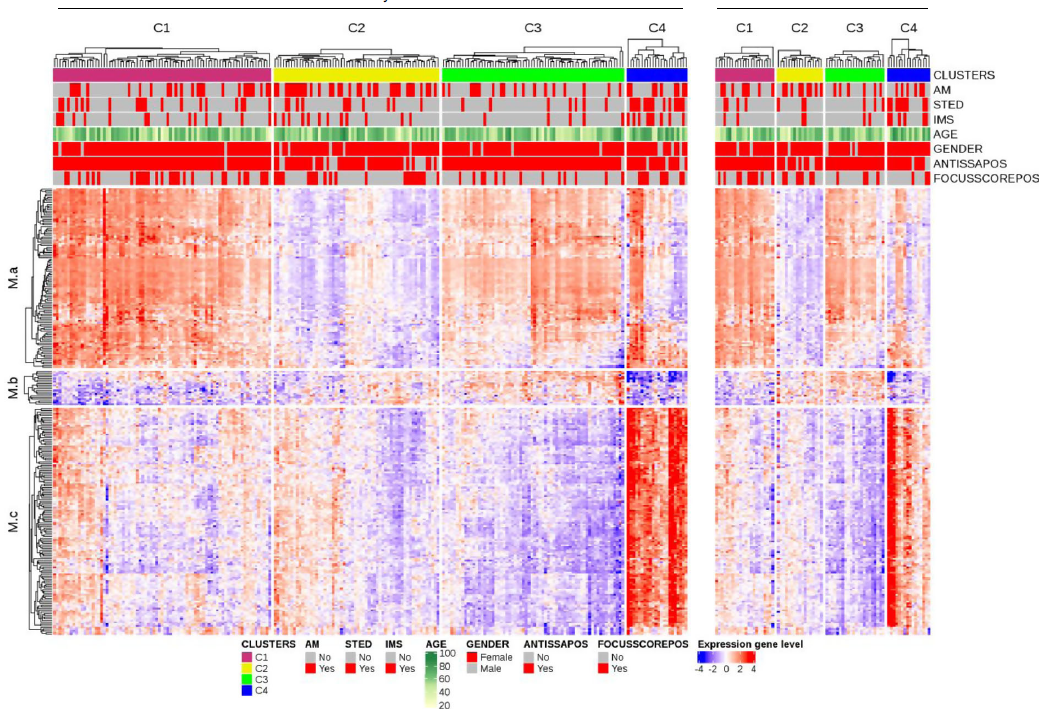
\includegraphics[width=\textwidth]{figures/sjogren/heatmap_sjogren.png}
         \caption[Heatmap performed for 304 pSS patients (Discovery set: 227, Validation set: 77) showing the distribution of gene transcripts.]{ In columns patients are grouped by cluster assignment and in rows genes are grouped by functional modules (three identified), with the \emph{discovery set} on the left and \emph{validation set} on the right. 
         The level of transcriptomic expression is encoded by a colour scale, a red colour depicting a stronger expression value. We also added at the top additional phenotype annotations: the treatment (AM: antimalarials, STED: steroids and IMS: immunosuppressors), age, gender, ANTISSAPOS as an indicator variable of the presence of anti-SSA/Ro antibody and finally FOCUSSCOREPOS as the discretised variable of the focus score \autocite{liao_etal22}.}
         \label{subfig:heatmap-sjogren}
     \end{subfigure}        
    \hfill
     \begin{subfigure}[p]{0.35\textwidth}
         \centering
         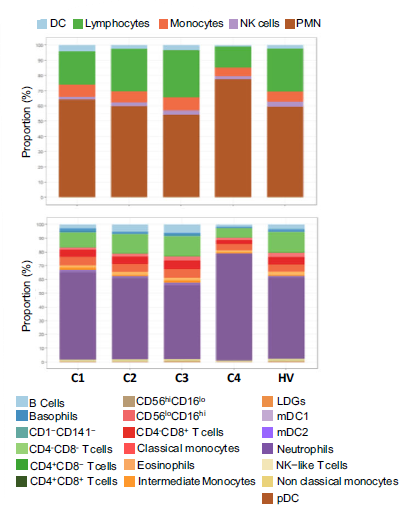
\includegraphics[width=\textwidth]{figures/sjogren/cellular_proportions.png}
         \caption[\textbf{Cell population composition in blood samples from the 4 identified clusters.}]{The bar chart denotes the cell types proportion per cluster, normalised to sum to one, as inferred from the gold-standard deconvolution algorithm Cibersort \autocite{newman_etal15}.}
         \label{subfig:cell-population-cibersort}
     \end{subfigure}
    \caption{Infographic of Chapter 4, about a practical use case of Gaussian mixture models applied to classify patients into groups with similar transcriptomic profiles.}
    \label{fig:infographic-sjogren-clustering}
\end{figure}
}

\chapter{Article 2: A new molecular classification in primary Sjögren’s syndrome}
\label{sec:sjogren-clustering}

% 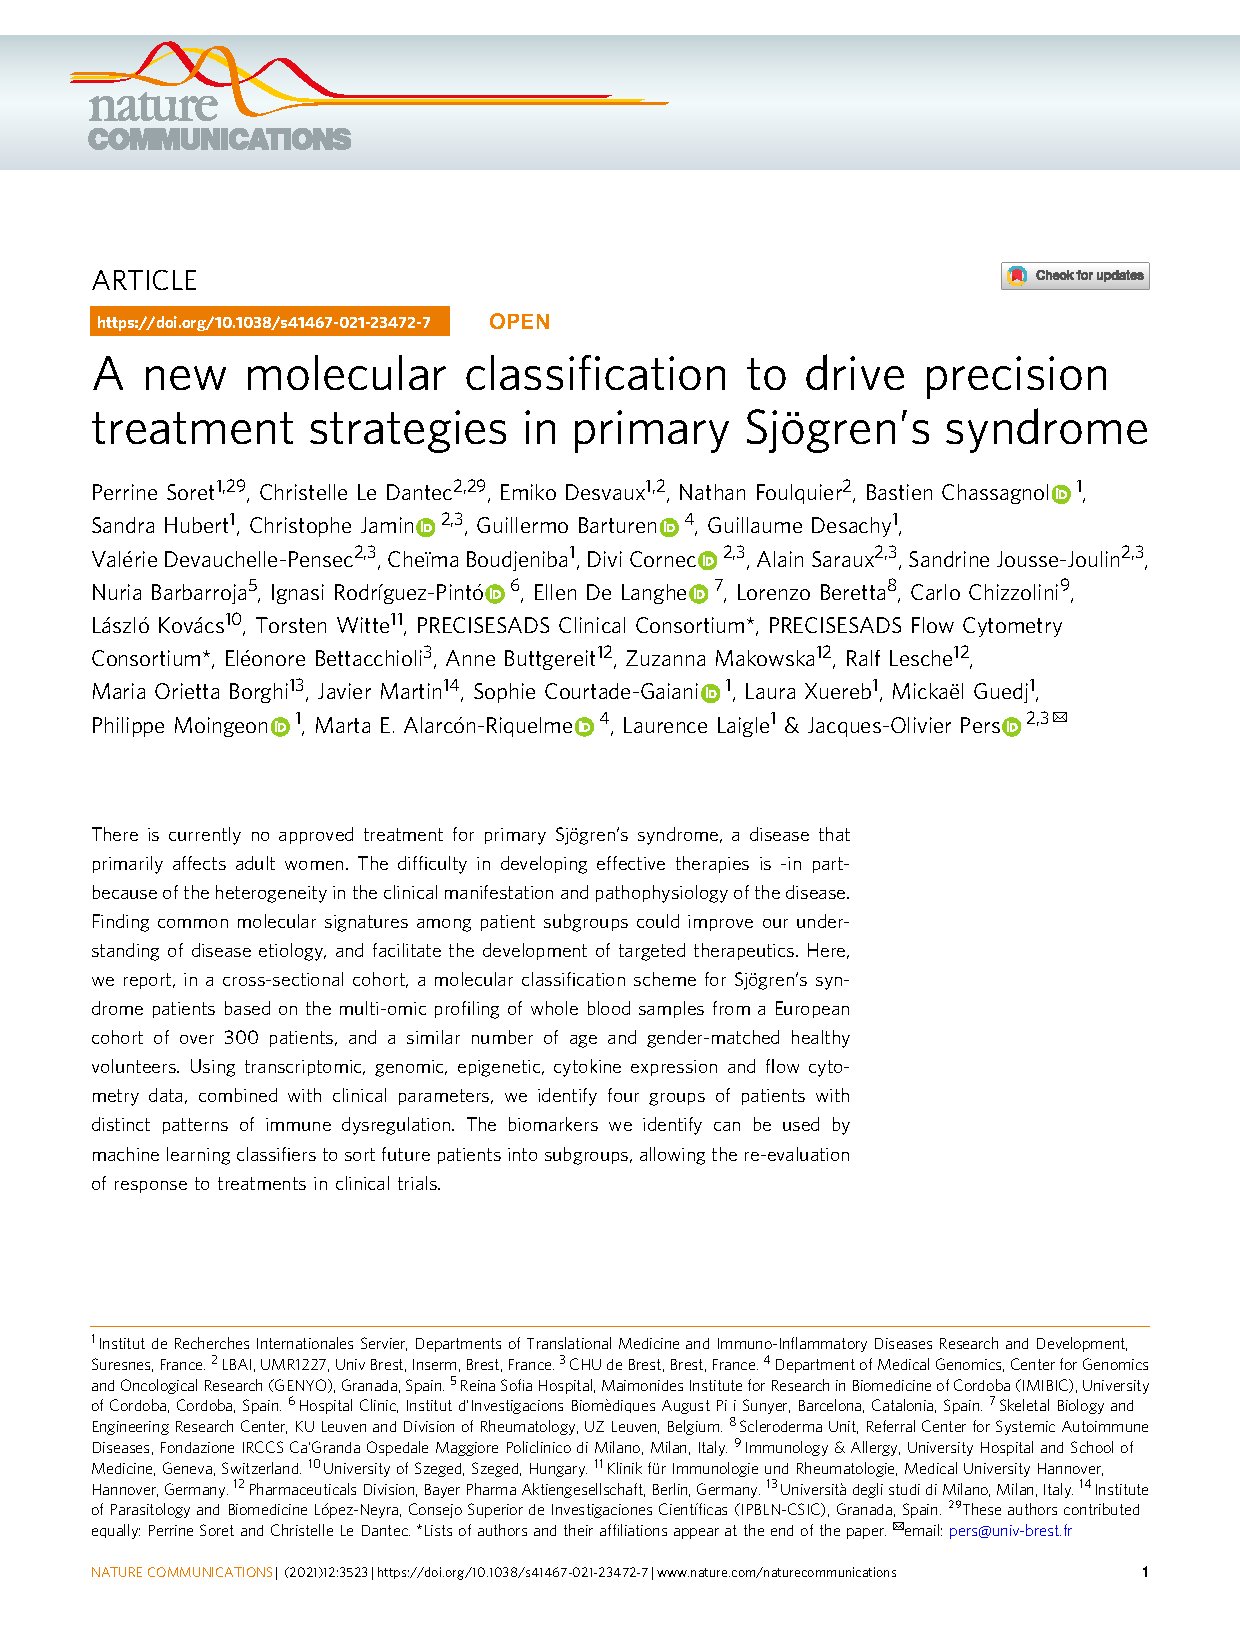
\includepdf[nup=2x1, pages={-}]{gmm_sjogren.pdf}

\section{Conclusion}

This study sheds light on the complex heterogeneity of pSS and contributes to unravel the intricate role of IFN pathways in its \emph{physiopathogenesis}. Besides, dissecting the heterogeneity of pSS patients should promote the development of targeted therapies and led to more personal and efficient clinical trials. However, further investigation is needed, including longitudinal studies to understand the stability of these clusters over time and the impact of treatments on gene signalling dysregulation. Furthermore, although collecting blood samples is a much easier task, it should be noted that most of the observed clinical features of Sjögren's disease, particularly in the early stages, are concentrated in the salivary glands, which may explains the lack of significant correlation between the observed clinical features and the patients grouped on the basis of transcriptomics.


I personally contribute to this paper through the following contributions:
\begin{itemize}
\item I participated to the standardisation and industrialisation of the RNASeq pipeline, and notably I contributed to the development of an unsupervised and statistically valid method to automatically discard the background transcriptomic noise, adjusting to the distribution nature of the transcriptomic data (see Details in Appendix \Cref{sec:truncated-distribution}).

\item I provided some insight and recommendations on the development of a consensual clustering method to identify patients sharing similar transcriptomic profiles. 

\item I ran and performed the statistical analyses to evaluate whether the cellular composition differs significantly between the identified clusters. Interestingly, not only we show strong heterogeneous cellular composition across patients, but it turns out that most of the transcriptomic variability observed could be explained by evolution of the cellular composition. \todo{add differences observed between the population of monocytes and B cells + cite cibersort again}
\end{itemize}

and detail in \Cref{sec:sjogren-extension} suggestions to perform co-clustering on both genes and patient samples.

\section{Perspectives}
\label{sec:sjogren-extension}

To extend this preliminary exploration study, I would certainly have adopted another method to establish a robust clustering of Sjögren's patients, without resorting to a combination of existing methods. Indeed, $k$-means and hierarchical clustering methods, are very similar in principle to Gaussian mixture models. Besides, we are rather used them for parameter initialisation, since they rely on additional and controversial assumptions (thus, both methods do not explicitly integrate the uncertainty of assignment to a given cluster, moreover, $k$-means assumes clusters of similar size and variability). Thus, it would certainly have been more interesting to assert the robustness of the model under different choices of Gaussian mixture model parametrisations (only the model with full covariance matrix structures has been tested) and number of components, using \emph{empirical bootstrap} (see also \Cref{chap:gmm-benchmark}, appendix sections \texttt{Model selection} and \texttt{Derivation of confidence intervals in GMMs} ). In addition, with bootstrap methods, we can easily derive confidence intervals, evaluating the statistical uncertainty on the parameters specific to each cluster. Finally, GMMs provide a straightforward manner to assign a posterior any observation, using directly the maximum a posteriori inferred from the parameters of the \acrshort{gmm} model, in place of a controversial correlation distance.
It's also worth noting that classical mixture models or $k$-means are not really suited to high-dimensional datasets, particularly when the number of variables (here genes, quantified by $G$) largely exceeds the number of observations, $N$. Projections on lower dimensional spaces, using for instance principal component analysis, and/or parsimonious parametrizations of the models (Appendix \Cref{sec:high-dimensional-simulations}) would certainly have enhanced the discrimination between the observed groups, while facilitating their visualisation and biological exploration, with a reduced computational cost.


Finally, and contrary to what we announced in the abstract, the qualification of multi-omic clustering is misleading, since we do not perform in practice \emph{integrated clustering} and based the classification of Sjögren's patients solely on transcriptomic data. Indeed, we use posterior analyses to annotate biologically these clusters (without, moreover, being able to correlate them significantly with clinical traits). We thus deemed that holistic approaches, genuinely integrating heterogeneous omic data and clinical features are particularly promising to disentangle the causal biological mechanisms and pathophysiology of these autoimmune diseases, which mostly elude us till now.

Integrated methods, combining several datasets of potential different nature, generally fall into the following categories: \textbf{early} (full), \textbf{late} (decision) or \textbf{intermediate} (partial) integration. Early integration methods involve combining all datasets into a single comprehensive dataset, which in turn is used as input for learning the model. However, this merging process requires representing the data in a common feature space, potentially leading to information loss. On the other hand, late integration approaches involve initially building individual models independently for each dataset and subsequently, combined them to generate an integrated model. However, this approach may not fully leverage the shared patterns present in the different datasets, potentially leading to suboptimal performance of the final integrated model.

We describe some of these integrated, network-based methods below:

\begin{itemize}

\item Similarity Network Fusion (SNF) \autocite{wang_etal14} combines networks using a diffusion process, but might struggle finding shared patterns for highly heterogeneous datasets. A quick overview of this method is further detailed in next \Cref{chap:sjogren-cheima}.

\item Variants of the \acrshort{nnmf} method might also be used to retrieve hidden structures shared across multiple datasets, projecting them into a smaller subspace, while enforcing the positivity constraint on gene or proteomic expression. Among these methods, we may quote Natural Gradient Weighted Simultaneous Symmetric NMTF (NG-WSSNMTF) \autocite{gligorijevic_etal16} or iCell (integrated Cell), a bottom-up,integrated model of cancer cells, relying on non-negative matrix tri-factorization (NMTF, \autocite{malod-dognin_etal19}).
For instance, iCell combines three molecular interaction networks: protein-protein interaction (PPI), gene co-expression (COEX), and genetic interaction (GI) networks and has been used to compare cancer-specific cell networks for breast, prostate and colorectal cancers along with their corresponding control tissues.  Precisely, in the iCell framework, each network, represented by its \emph{adjacency matrix}, is decomposed into two matrices: one common that groups genes into clusters shared across all decompositions, and one compact, low dimensional representation of each omic network, describing how the gene clusters relate specifically to each other in it. The decomposition is achieved by minimising the Frobenius norm of the difference between the original adjacency matrix and the factorial decomposition product specific to each network, using an iterated, fixed-point method (an explicit formula returning the roots being unreachable, instead a local optimal solution is computed). Finally, a final threshold process refines the network by discarding the bottom $99\%$ of the lowest pairwise transcriptomic relationships. Interestingly, while the standard differential mean expression, especially on cohorts of relatively small sizes and thus lacking of statistical power, failed at retrieving varying gene expression between cancer and control cases, iCell methodology succeeds in exhibiting significantly altered \emph{wiring patterns}, namely the crosstalk patterns of transcriptomic interactions.

\item Spectral clustering on multi-layer graphs (SC-ML) \autocite{dong_etal14} and GraphFuse \autocite{papalexakis_etal13} are both spectral methods, but may undergo poor cluster convergence or struggle with memory issue \autocite{malod-dognin_etal19}. The key idea behind spectral clustering is to project the data into a lower-dimensional subspace, by computing and keeping the largest eigenvectors of the corresponding Laplacian operator of the adjacency matrix, enhancing thus the separation between the clusters. Fllowing this dimension reduction, any clustering algorithm (usually $k$-means) applied to the transformed data can be used to assign each data point to a specific cluster, however, like most clustering methods, there is no universal method to derive the number of clusters. Spectral clustering is particularly useful when the underlying structure of the data is highly intricate, since it can reveal nonlinear patterns and complex relationships between data points. However, it requires careful parameter tuning and can be computationally demanding for large datasets. 

\item Markov Clustering (MCL) \autocite{enright_etal02} is a single graph clustering method that requires at first merging all omics networks into one structure, and then clustering the resulting union graph. It relies on the idea that the asymptotic distribution of random walks on a graph reflects the degree of interaction relating two distant clusters.
\end{itemize}

However, we should point out that these integrated methods, due to the large, intractable network sizes, the potential presence of spurious and noisy pairwise edges and possibly the lack of shared biological mechanisms among several omics, struggle to converge into consistent and shared interaction patterns solutions. It may lead for instance to poor overlap between the identified clusters  across several cohorts from the same disease or even returns to an empty set of candidate solutions. Hence, a trade-off has to be found between integrating datasets of different nature, using prior knowledge, and focus on returning a robust and highly predictive model. This issue has been partly addressed in the following paper, , where the purpose was to determine the perfect balance between improving the accuracy and reproducibility of gene regulatory network inference while integrating prior knowledge datasets using transcription factor binding sites as proxy of gene interaction candidates. It turns out that only one third of the prior putative pairwise interactions significantly improved the predictability performance of the network, while others have no impact, or even worse impact the overall performance.


\leadchapter{In this paper, we intended to understand the heterogeneity of patients suffering from pSD and deciphering the intertwined transcriptomic interactions by identifying larger gene modules summarising transcriptome expression.

We identified 13 Consensus gene Modules (CMs) that contribute the most to the variability of the transcriptome across pSD patients. We retrieved them using unsupervised clustering methods on four different transcriptomic datasets, all processes from blood samples. Then, gene set enrichment analyses were used to annotate each module based on its connection with cell populations or biological function. Finally, flow cytometry data and cytokine measurements were used to validate biologically the annotations. \Cref{fig:infographic-louvain-clustering} details the major steps of the clustering pipeline, as well as the major biological results. 


Precisely, the four datasets proceed from private sources funded by the NECESSITY consortium (ASSESS \autocite{gottenberg_etal13}, PreciseSADS \autocite{barturen_etal18} and UKPSSR \autocite{ng_etal11}) or publicly available repositories, such as GSE84844 \autocite{tasaki_etal17}. To reduce partly the intrinsic high dimensionality of transcriptomic data \footnote{with \num{20000} identified genes coding for proteins, the number of pairwise interactions covers the staggering number of  \num{4.e8} correlation coefficients}, often prone to high confusing technical noise, we tailored a dedicated analysis workflow, summarised in \Cref{subfig:cheima-pipeline}.

Initially, each cohort's gene expression matrix was transformed into an affinity matrix representing the gene co-expression network. Each pairwise Pearson correlation coefficient was mapped to a non-linear but monotonic \emph{sigmoid function}, resulting in lower correlation coefficients being shrunk towards zero \autocite{wang_etal14}. Subsequently, an additional filtration step enables to further prune the built network and keep only highly co-expressed genes, generating a strongly sparse weighted graph. Secondly, we used the \acrfull{snf} algorithm (\autocite{wang_etal14} and \Cref{subfig:snf-method}) to emphasise shared network patterns and merge multiple affinity matrices across the four independent cohorts of pSD patients' blood.

Finally, we applied Louvain clustering \autocite{blondel_etal08} to this sparse, \emph{consensus graph} and identified 13 CMs. In brief, Louvain's method is one of the graph clustering algorithms that focuses on maximising the \emph{modularity} of the network. This metric, bounded between -1 and 1, aims at computing the averaged density of edges within clusters with respect to the interaction density between communities, a graph composed only of \textit{cliques} unconnected to each other displaying a score of 1. However, Louvain's paper implements two innovative features: an approximate heuristic algorithm, briefly described in \Cref{subfig:louvain-method} to increase the scalability of the method to larger datasets (it has even been applied to social network, with tens of millions of user nodes) and an internal hierarchical approach, enabling to adjust the level of granularity to user requirements.

\begin{figure}
     \centering
     \begin{subfigure}[p]{0.6\textwidth}
         \centering
         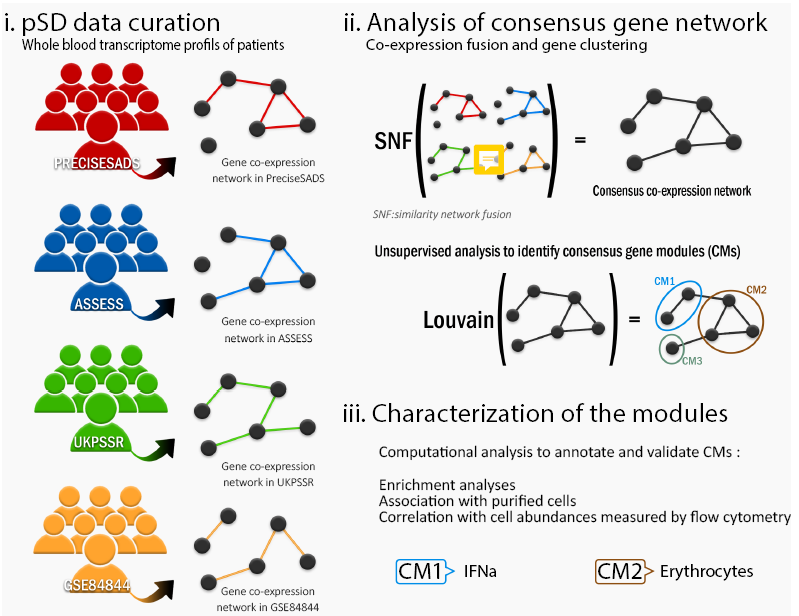
\includegraphics[width=\textwidth]{figures/cheima_pipeline.png}
         \caption{Schematic representation of the pipeline used in this paper, in which step i) encompasses all the construction steps to retrieve an individual similarity network, ranging from the preprocessing and data wrangling operations to the pruning of spurious correlations, step ii) covers the network and clustering operations to return consensual modules across all studied datasets and iii) includes all the post statistical and biological experiences to assert the soundness and relevance of the returned gene clusters.}
         \label{subfig:cheima-pipeline}
     \end{subfigure}
     \vfill
     \begin{subfigure}[p]{0.4\textwidth}
         \centering
         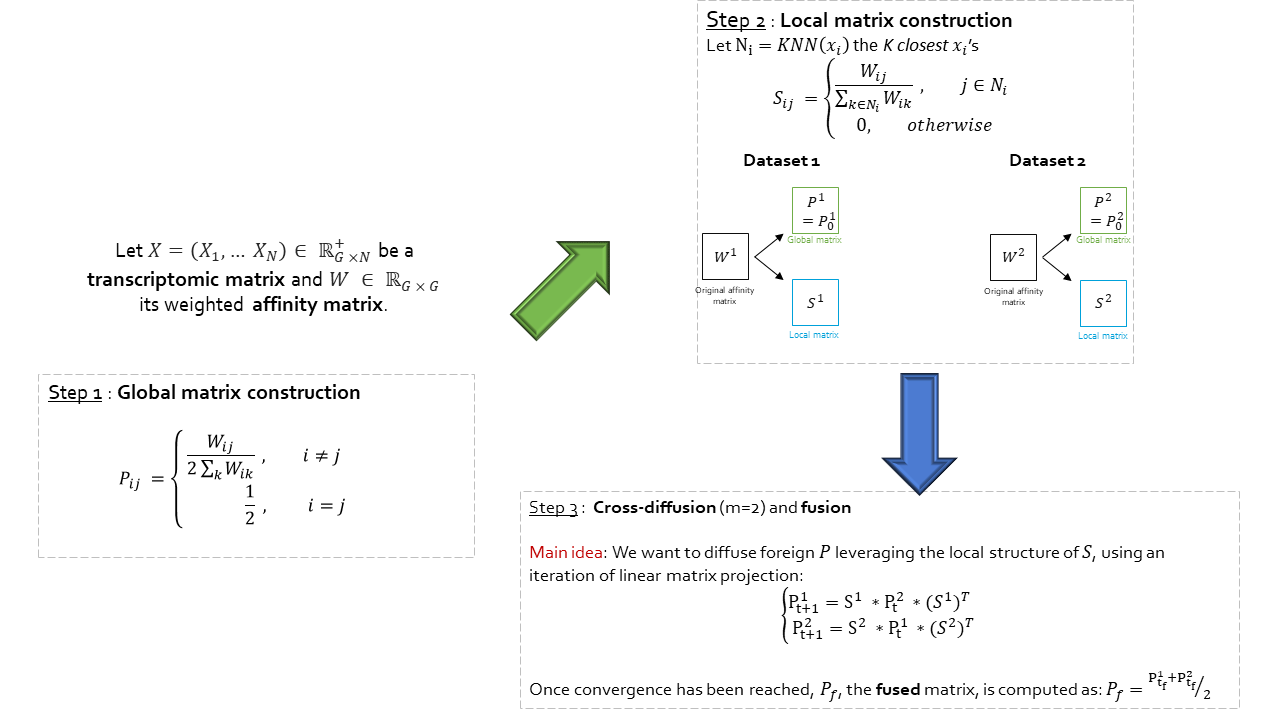
\includegraphics[width=\textwidth]{figures/similarity_network_fusion.png}
         \caption{\acrshort{snf} [\autocite{wang_etal14}] is a \emph{cross-diffusion} process that outputs enhanced metrics by averaging in an integrated manner multiple similarity measures. Briefly, it consists first of computing similarity matrices for each dataset, one \emph{global} and one \emph{local}, discarding remote nodes. Then, iterative steps of matrix projection on the same endomorphic graph space and a final averaged operation results in a fused global network that concatenates relevant neighbourhood information across all datasets.}
         \label{subfig:snf-method}
     \end{subfigure}
     \hfill
     \begin{subfigure}[p]{0.4\textwidth}
         \centering
         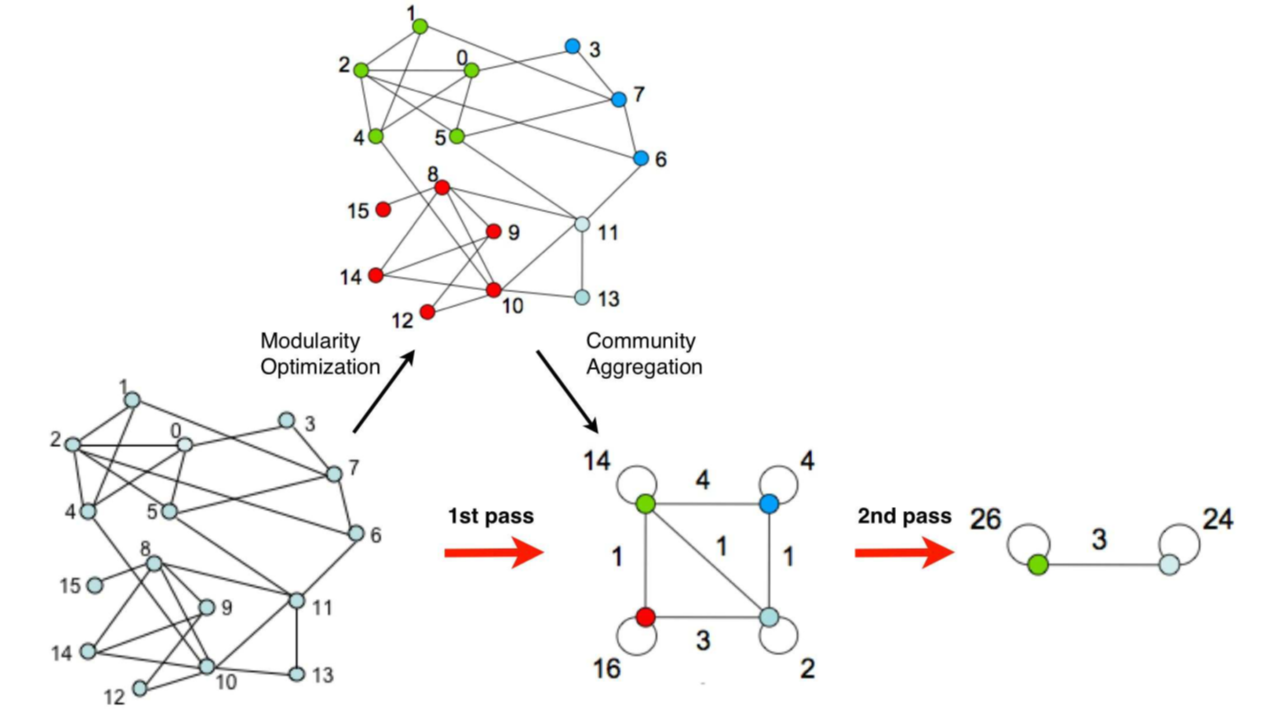
\includegraphics[width=\textwidth]{figures/louvain_clustering.png}
         \caption{A schematic visualisation of Louvain's algorithm \autocite{blondel_etal08} each pass (alternatively \emph{epoch}) is made of two phases: a local optimisation phase, where modularity is increased only by local changes of community assignment followed by an aggregation phase, where sub-communities are merged in order to build a global network of clusters. The passes are repeated iteratively until the total modularity score no longer increases.}
         \label{subfig:louvain-method}
     \end{subfigure}        
    \vfill
     \begin{subfigure}[p]{0.4\textwidth}
         \centering
         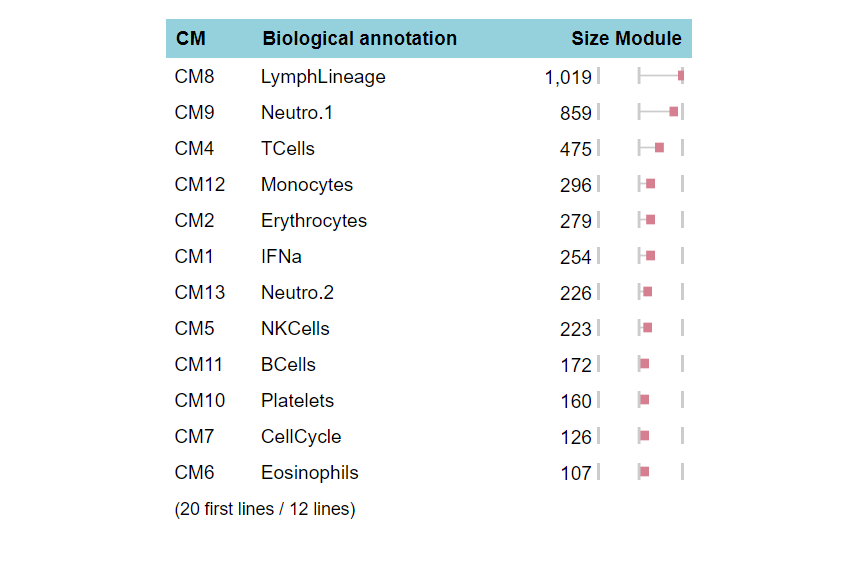
\includegraphics[width=\textwidth]{figures/cheima_modules.png}
         \caption{13 consensus modules have been identified between the studied datasets, and we were able to annotate consistently 12 of them with either metabolic pathways or cellular-related mechanisms represented in the following table. Voluntarily, we discard module CM3, since it strongly diverges between datasets.}
         \label{subfig:cheima-modules}
     \end{subfigure}
     \hfill
     \begin{subfigure}[p]{0.4\textwidth}
         \centering
         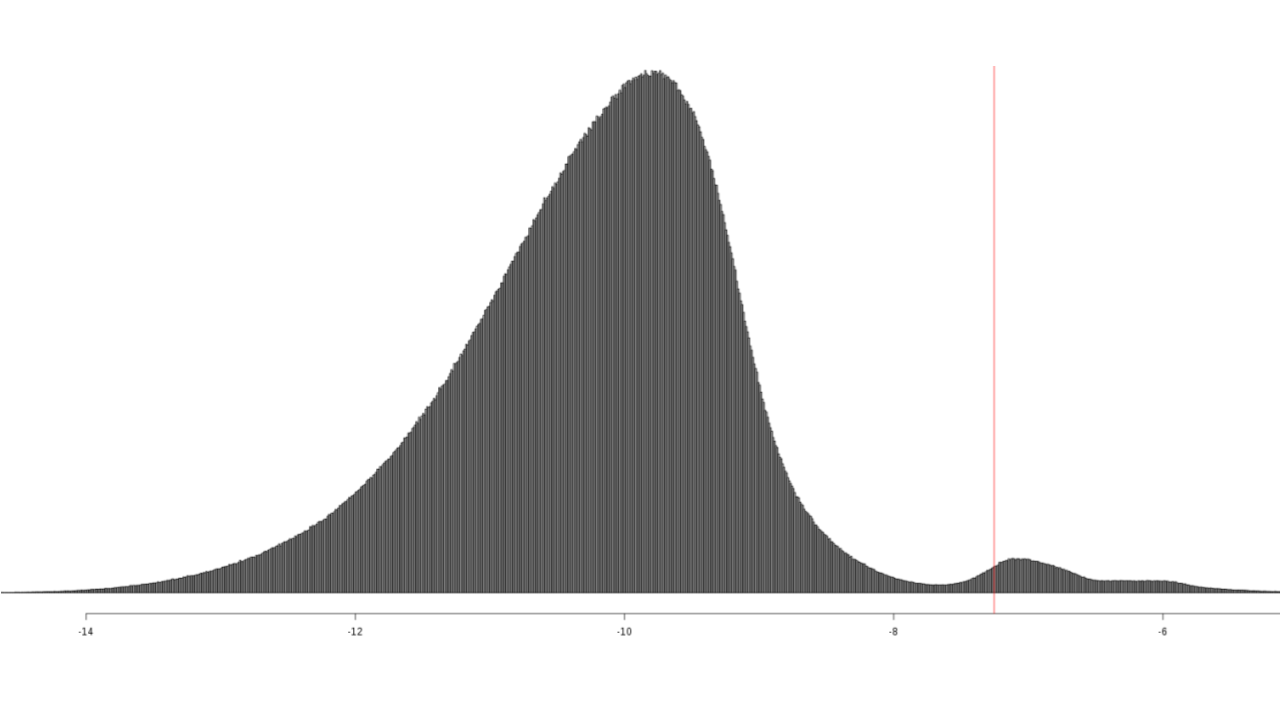
\includegraphics[width=\textwidth]{figures/distribution_weights_snf.png}
         \caption{Histogram showing the distribution of correlation weights in the total \acrshort{snf} matrix. We fit a mixture of positively skewed Gaussian distributions and uses the $0.05^\text{th}$ quantile of the second mode of the distribution, visualised by  the vertical red line, as the signal upper threshold to discard irrelevant weights.}
         \label{subfig:weight-snf}
     \end{subfigure}    
    \caption{Infographic of Chapter 5, about a practical use case of high dimensional clustering, to identify shared gene modules across technical batches.}
    \label{fig:infographic-louvain-clustering}
\end{figure}

Performing the same clustering independently on each cohort, keeping the same hyper-parameters confirm that these CMs are highly consistent, no matter the origin of the dataset. Notably, we found out that CM1 was correlated with type 1 interferon signalling, CM7 corroborates cell cycle-related genes and out of the 11 remaining, 9 modules were significantly enriched in different lymphoid and myeloid cell subsets \Cref{subfig:cheima-modules}. In addition, the identified CMs were then compared against two previous stratifications of gene expression, and we were able to recover significant overlap in the clusters assignment performed by both approaches. Nonetheless, we should point out that the module displaying the highest number of genes ($n=1247$) and the lowest averaged expression value showed inconsistent biological characterisation and was assimilated to a nuisance cluster, a commonly observed artefact in omics clustering papers \todo{refer to papers discussing this issue}.
We also looked into the therapeutic effect of a drug combination of hydroxychloroquine and leflunomide on the blood transcriptome of pSD patients and revealed that the expression of some modules was significantly linked to treatment outcome, suggesting these modules could be leveraged as predictive biomarkers.


While the construction of the main bricks of the pipeline and the biological exploitation of the results was mostly supervised by my co PhD Cheima, I mostly contribute to this paper with the following tasks:

\begin{itemize}
\item With the \acrshort{bbc} team, we have released an user-friendly, standardised and internal pipeline dedicated to the pre-processing, normalisation and downstream analysis of transcriptomic datasets, discussed in further details in \Cref{chap:transcriptome-workflow}.

\item Precisely, unsupervised clustering methods, adjusted to fit the nature and the shape of the density distribution of transcriptomic datasets, which may strongly differ with respect to the normalisation method chosen, were intensively used to automatically set apart noisy genes from highly expressed transcripts, as well as to automate the decision threshold to prune irrelevant edge (see \Cref{subfig:weight-snf}).

\item Finally, while several clustering methods have been benchmarked to identify closely related transcript networks, it turns out that the Gaussian mixture approach underperformed compared to the Louvain's method, yet, several assumptions underlying standard Gaussian mixtures were not met, namely that the number of observations, here the genes, largely exceeds those the number of variables, here the biological samples, and variants of \acrshort{gmm}, such as parsimonious parametrisations or projection to sub-dimensional space, as detailed in Appendix \Cref {sec:high-dimensional-simulations}, combined with strong refinement of the parameters and the number of components, might have improved the results. In addition, correlation data sets, by exhibiting naturally limited values, do not follow in general Gaussian distributions, with bell-shaped and symmetrical graphical representations.

\end{itemize}
}

\chapter{Article 3: Gene clustering applied to primary Sjögren’s disease}
\label{chap:sjogren-cheima}

%\includepdf[nup=2x1, pages={-}]{spectral_clustering.pdf}

\section{Conclusion}
\label{sec:conclu-gene-modules}

In summary, this study revealed that 13 gene modules over a starting collection of \num{4196} genes were enough to capture most of the heterogeneity of the blood transcriptome in pSD patients. We were able to further annotate these modules with various cell types and biological functions, providing insights into the pathophysiology of pSD. 
In addition, we suggest using these modules as biomarkers for patient stratification and prediction of treatment response in DBP. However, further clinical validation trials are required to fully understand the relevance of these genetic modules in identifying the causal mechanisms involved in disease progression.

\chapter{RNA-Seq workflow}
\label{chap:transcriptome-workflow}

\todo{Nextflox pipeline; \url{https://www.nature.com/articles/s41598-020-76881-x}, figure 1 notamment pour d'autres exemples de pipeline globales}
% \section{An automated Nextflow pipeline for genome alignement}
%\subsection{Bioinformatic tools for genome alignment}


\section{Objectives} 

\begin{itemize}
\item
  Identification of a \emph{reference signature} matrix, enabling to discriminate specifically any of the cell populations that may contribute to the observed bulk transcriptomic expression.
\item
  Evaluation of the impact of confusing technical and environmental variables on the individual cell transcriptomic expression, such as the effect of the sequencing method, the disease, the gender or the age of the patient.
\end{itemize}


\section{Gene expression databases} 
\label{gene-expression-databases}


\subsection{Import relevant files} 
\label{import-relevant-files}

Most of high-throughput transcriptomic datasets are available on two public repositories: NCBI \emph{Gene Expression Omnibus (GEO)} and ECBI \emph{ArrayExpress.}

GEOs objects are stratified with the following hierarchical structure:

\begin{enumerate}
\item
  A \emph{Platform} object details the general sequencing protocol and lists the probes or gene annotations. Besides, it gathers all the experiences that have been performed under this specific sequencing method. Platform ID follows the following notation: GPL, followed with an accession number.
\item
  A \emph{Series} object identifies a set of Samples associated with the same biological experiment and additionally summarises phenotype features and the global design. It is idnetified with the GSExxx flag.
\item
  A \emph{Sample} record, identified as GSMxxx, describes the conditions under which an individual Sample was handled, the manipulations it undergoes like the platform used, and the abundance measurement of each annotated transcript.
\end{enumerate}

The second biggest source of public datasets is \emph{ArrayExpress}, with differs from GEO with additional restrictions on the format of the datasets submitted, imposing to make them MIAME-compliant. Currently, 76,635 studies are represented in the ArrayExpress compendium. The general format is for each repository, a zipped MAGE-TAB document which splits itself into an \emph{Investigation Description Format (IDF)} file, equivalent to the MIAME experimental data of the eset object and describing top-level protocol experiences: \href{https://rdrr.io/pkg/Biobase/man/abstract.html}{\texttt{Biobase::experimentData}}, \emph{Array Design Format (ADF)}, equivalent to the feature data: \href{https://rdrr.io/pkg/Biobase/man/featureData.html}{\texttt{Biobase::fData}}, with the position (for microarray only) and the annotation of the measured transcripts, \emph{Sample and Data Relationship Format (SDRF)}, equivalent to the phenotype data: \href{https://rdrr.io/pkg/Biobase/man/phenoData.html}{\texttt{Biobase::pData}} and eventually the raw and processed data files, that store transcriptomic expression.

While the packages \href{http://seandavi.github.io/GEOquery/articles/GEOquery.html}{\texttt{GEOquery}}, \autocite{R-GEOquery}, \autocite{GEOquery2007}, and \href{https://bioconductor.org/packages/release/bioc/vignettes/ArrayExpress/inst/doc/ArrayExpress.pdf}{\texttt{ArrayExpress}}, \autocite{R-ArrayExpress}, \autocite{ArrayExpress2009}, have been designed to automatically query and fetch online databases, they are rather restricted to a specific format, unfortunately rarely met in practice. Depending on the level of precision required, along with general feature description files, we let the user to choose between raw or pre-processed data (generally, a tab-delimited file enumerating for each probe or identified transcript its total expression). In practice, one of the major bottlenecks is the absence of pre-processed expression data in the majority of RNASeq experiments, and the lack of standardisation of raw datasets. We have therefore attempted to partially resolve these limitations by respectively developing proprietary functions \texttt{bbcFetching::import\_normalised\_data} and \texttt{bbcFetching:::import\_raw\_files} for normalised and raw datasets, both functions attempting at first to parse local files, then fetch them online, and finally homogenises the output into an ExpressionSet object:

In addition, we display respectively the architecture of ArrayExpress, GEO and SRA databases\footnote{This last repository is specifically dedicated to store high throughput sequencing experiments, and reveals its full potential as un unlimited and parallel data storage, at the raw read alignment level, along with NCBI GEO and EBI ArrayExpress databases. Currently, the R package \href{http://www.ncbi.nlm.nih.gov/books/NBK47537/}{SRAdb}, \autocite{R-SRAdb}, \autocite{SRAdb2013}, is recommended for automatically querying, downloading and extracting alignment information}, in Fig.\Cref{fig:databases-schema-pdf}.

\begin{figure}

{\centering \subfloat[Relation database and user API interface, from  \href{https://ecoliwiki.org/colipedia/index.php/Gene_Expression_Omnibus_(GEO)}{Wiki GEO} 
\label{fig:databases-schema-pdf-1}]{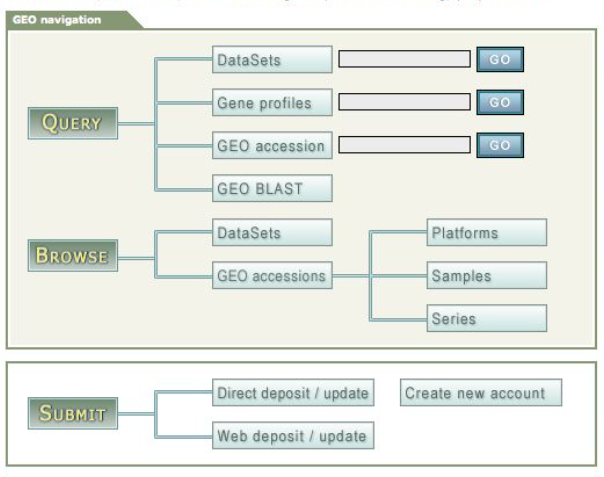
\includegraphics[width=0.45\linewidth]{figures/ERD_GEO} }\subfloat[The \href{https://www.bioconductor.org/packages/release/bioc/vignettes/SRAdb/inst/doc/SRAdb.pdf}{ArrayExpress} architecture, with user functionality detailled at the bottom on its vignette.\label{fig:databases-schema-pdf-2}]{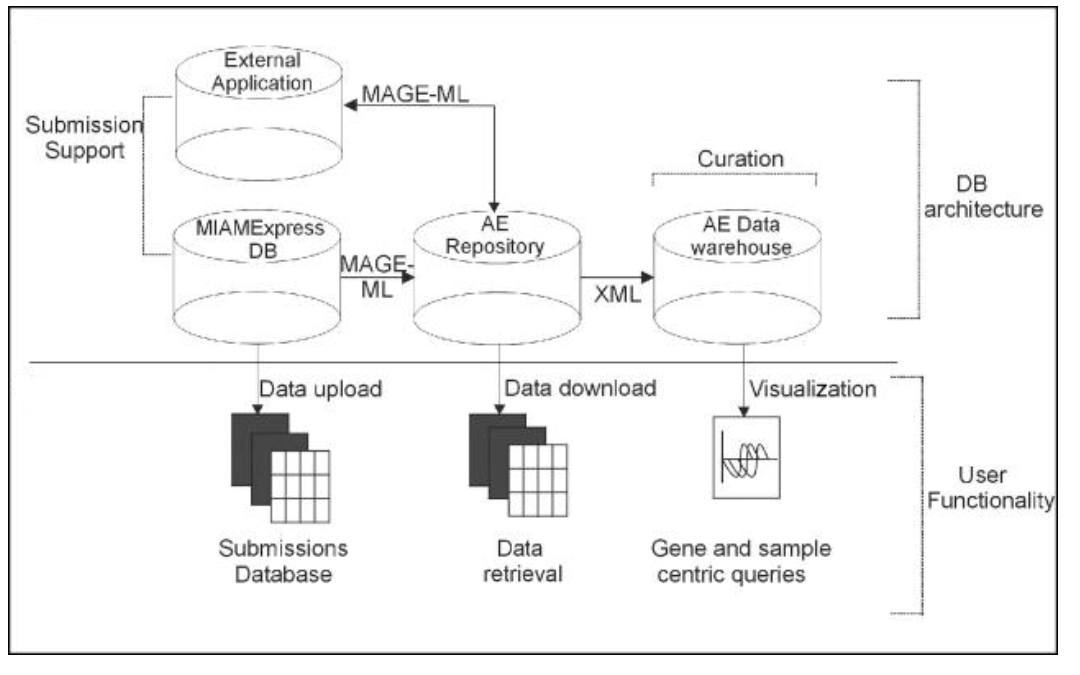
\includegraphics[width=0.45\linewidth]{figures/ERD_ArrayExpress} }\newline\subfloat[The graphical representation describing the entity relationships between the tables in \href{https://www.bioconductor.org/packages/release/bioc/vignettes/SRAdb/inst/doc/SRAdb.pdf}{SRAdb vignette}\label{fig:databases-schema-pdf-3}]{\includegraphics[width=0.45\linewidth]{figures/ERD_SRAdb} }

}

\caption{We display respectively the ERD (\emph{Entity-Relationship Diagram}), of GEO, ArrayExpress and SRA databases}\label{fig:databases-schema-pdf}
\end{figure}


\subsection{Data wrangling with ExpressionSet}\label{data-wrangling-with-expressionset}

An ExpressionSet object is composed of an expression matrix, a gene annotation dataset
and a phenotype dataset storing patient information, associated with general metadata stored in a MIAME object. In this section, we enumerate all the data formatting and quality check-ups performed to clean and leverage essential information from ExpressionSet:

\begin{enumerate}
\def\labelenumi{\arabic{enumi}.}
\item
  Data format: We require that transcriptomic expression is stored in a matrix, and that the annotation sets are \texttt{data.frame} objects.
\item
  All elements composing the eset must be documented with colnames and rownames, such that the colnames of the eset match the rownames of the \texttt{pData} object (correspond to unique identification of samples) and its rownames match the rownames of the \texttt{fData} object (unique identification of transcripts). We recall the general structure of ExpressionSet objects as well as the operations required to manipulate them in in Fig.\Cref{fig:databases-schema-pdf}.
\item
  Variable types: carefully prepare samples and features annotation data by formatting numerical variables in numeric format and converting textual variables as factors. When comparing several eset objects, it is relevant to keep track of factor assignment, and homogenises them across batches. About missing values, we marked unequivocally using the \emph{reserved variable name} \texttt{NA}, see sub\Cref{subsubsec:sample-annotation} for details.
\item
  Gene annotation: this step ensures that gene ID used can be uniquely mapped to their corresponding most updated HGNC symbol. We can additionally filter out genes that are not involved in any of the biological functions of interest, see details in sub\Cref{subsubsec:gene-annotation}.
\item
  (Optional) There is currently a strong lack of standard nomenclature to refer to cell types. We thus provide in sub\Cref{subsubsec:cell-type-annotation} helper functions to homogenise them across samples. Similarly, we may as well use ontologies to uniquely identify diseases or tissues.
\end{enumerate}





\begin{figure}

{\centering \subfloat[Structure of a \href{https://www.researchgate.net/figure/Structure-of-Bioconductors-ExpressionSet-class_fig1_326163413}{Bioconductor's ExpressionSet} object \autocite{Biobase2015}--\autocite{klaus_reisenauer18}.\label{fig:expressionset-structure-pdf-1}]{\includegraphics[width=0.45\linewidth]{figures/expressionset_structure} }\subfloat[The \href{https://combine-australia.github.io/2017-05-19-bioconductor-melbourne/data_structures.html}{SummarizedExperiment} object \autocite{R-SummarizedExperiment} is a generalisation of ExpressionSet. It is traditionally used to store the results of several experiences (provided at least some Gene IDs match). Besides, this format is required in some normalisation and differential analysis functions, notably for the \emph{vst} normalisation applied by \href{https://bioconductor.org/packages/release/bioc/vignettes/DESeq2/inst/doc/DESeq2.html}{DeSeq2} Bioconductor package \autocite{R-DESeq2}, \autocite{DESeq22014}.\label{fig:expressionset-structure-pdf-2}]{\includegraphics[width=0.45\linewidth]{figures/summarised_experiment_structure} }

}

\caption{General structure of the objects most commonly used in R to store transcriptomic data}\label{fig:expressionset-structure-pdf}
\end{figure}


\subsubsection{Sample annotation} 
\label{subsubsec:sample-annotation}

Part of this tedious data cleaning is automatically carried out with function \href{https://rdrr.io/pkg/bbcWrangling/man/clean_eset_names.html}{\texttt{bbcWrangling::clean\_eset\_names()}}, which proceeds in three steps:

\begin{enumerate}
\def\labelenumi{\arabic{enumi}.}
\item
  First, simplify the identification colnames of objects \href{https://rdrr.io/pkg/Biobase/man/phenoData.html}{\texttt{Biobase::pData}} and \href{https://rdrr.io/pkg/Biobase/man/featureData.html}{\texttt{Biobase::fData}}, mostly by complying them with the ruling names' syntax of R.
\item
  All non-ascii characters can be trimmed, however, perform this operation with care, since some of the characters of gene names may not comply with ASCII character encoding format.
\item
  The most useful function, removes any constant colname of object \texttt{Biobase::pData()}, and stores it as a \texttt{MIAME} object in slot \texttt{Biobase::experimentData}. We mean by \emph{constant} any column that stores information common to all the samples, or patients, considered for the experiment, which can be typically the sequencing technology, the general experimental name or setting, or general information about laboratory and biologists contacts.
\end{enumerate}

In addition to simplify the manual curation of phenotype data, these general management operations help identifying variables of interest, as well as confusing variables (for instance, batch replicates), and reduces the storage space taken by the eset object. For instance, the size taken by the phenotype dataset in memory hardware shifts from 322.8 Kb and 64, to 228 Kb and 26 on the cleaned eset.

However, while part of the automated data curation is performed by \href{https://rdrr.io/pkg/bbcWrangling/man/clean_eset_names.html}{\texttt{bbcWrangling::clean\_eset\_names()}}, there is still a need of manual curation, and we displayed below some common data wrangling operations to be performed on purified cell expression sets, respectively for GEO ID 149050 and 137143:

\begin{itemize}
\item
  Rename columns, such that shared phenotype information, are labelled consistently across several Expression Sets, for instance the columns returning the cell assignement or the patient id
\item
  Convert to factor any categorical variable which may contribute to biological or technical variability, since they will be required for batch correction and downstream analysis. Perform similarly for continuous values. For the last two experiences described, we identified three shared categorical variables of interest: patient assignment, cell type assignment and disease phenotype, and one continuous variable, age of the patient.
\item
  About categorical variables, you may attempt to merge closely related cell factors to gain statistical power and promote comparison across samples, a point further developed in sub\Cref{subsubsec:cell-type-annotation}
\end{itemize}

\begin{Shaded}
\begin{Highlighting}[]
\NormalTok{gse149050\_pheno\_data }\OtherTok{\textless{}{-}}\NormalTok{ Biobase}\SpecialCharTok{::}\FunctionTok{pData}\NormalTok{(gse149050\_raw\_count\_clean) }
\NormalTok{gse149050\_pheno\_data }\OtherTok{\textless{}{-}}\NormalTok{ gse149050\_pheno\_data  }\SpecialCharTok{\%\textgreater{}\%}
\NormalTok{  dplyr}\SpecialCharTok{::}\FunctionTok{select}\NormalTok{(}\FunctionTok{c}\NormalTok{(}\StringTok{"geo\_accession"}\NormalTok{,}
                  \StringTok{"age\_ch1"}\NormalTok{, }\StringTok{"cell\_type\_ch1"}\NormalTok{,}
                  \StringTok{"patientuid\_ch1"}\NormalTok{, }\StringTok{"relation\_1"}\NormalTok{,}
                  \StringTok{"disease\_state\_ch1"}\NormalTok{)) }\SpecialCharTok{\%\textgreater{}\%}
\NormalTok{  dplyr}\SpecialCharTok{::}\FunctionTok{rename}\NormalTok{(}\AttributeTok{sample\_id=}\StringTok{"geo\_accession"}\NormalTok{, }\AttributeTok{disease=}\StringTok{"disease\_state\_ch1"}\NormalTok{) }\SpecialCharTok{\%\textgreater{}\%}
\NormalTok{  dplyr}\SpecialCharTok{::}\FunctionTok{rename\_with}\NormalTok{(}\SpecialCharTok{\textasciitilde{}}\FunctionTok{gsub}\NormalTok{(}\StringTok{"\_(ch)*1$"}\NormalTok{, }\StringTok{""}\NormalTok{, .x)) }\SpecialCharTok{\%\textgreater{}\%}
\NormalTok{  dplyr}\SpecialCharTok{::}\FunctionTok{mutate}\NormalTok{(}\AttributeTok{patient\_id=}\NormalTok{stringr}\SpecialCharTok{::}\FunctionTok{str\_extract}\NormalTok{(patientuid,}
                                                \AttributeTok{pattern =} \StringTok{"\^{}[[:upper:]]\{1\}[[:digit:]]+"}\NormalTok{),}
                \AttributeTok{disease=}\NormalTok{forcats}\SpecialCharTok{::}\FunctionTok{fct\_collapse}\NormalTok{(}\FunctionTok{as.factor}\NormalTok{(disease),}
                                              \AttributeTok{hc=}\FunctionTok{c}\NormalTok{(}\StringTok{"healthy control"}\NormalTok{),}
                                              \StringTok{"sle"}\OtherTok{=}\FunctionTok{c}\NormalTok{(}\StringTok{"systemic lupus erythematosus (SLE)"}\NormalTok{)),}
                \AttributeTok{age=}\FunctionTok{as.numeric}\NormalTok{(age), }
                \AttributeTok{URL=}\NormalTok{stringr}\SpecialCharTok{::}\FunctionTok{str\_extract}\NormalTok{(relation, }\AttributeTok{pattern =} \StringTok{"(?\textless{}=SRA: )(.*?)$"}\NormalTok{),}
                \AttributeTok{platform=}\StringTok{"GPL16791"}\NormalTok{, }\AttributeTok{tissue=}\StringTok{"blood"}\NormalTok{,}
                \FunctionTok{across}\NormalTok{(}\FunctionTok{c}\NormalTok{(}\StringTok{"cell\_type"}\NormalTok{, }\StringTok{"disease"}\NormalTok{, }\StringTok{"patient\_id"}\NormalTok{),}
                       \SpecialCharTok{\textasciitilde{}}\NormalTok{ janitor}\SpecialCharTok{::}\FunctionTok{make\_clean\_names}\NormalTok{(.x, }\AttributeTok{allow\_dupes =} \ConstantTok{TRUE}\NormalTok{) }\SpecialCharTok{\%\textgreater{}\%}
\NormalTok{                         forcats}\SpecialCharTok{::}\FunctionTok{as\_factor}\NormalTok{())) }\SpecialCharTok{\%\textgreater{}\%}
  \FunctionTok{select}\NormalTok{(}\SpecialCharTok{{-}}\FunctionTok{c}\NormalTok{(patientuid, relation, URL))}
\NormalTok{gse149050\_raw\_count\_clean }\OtherTok{\textless{}{-}}\NormalTok{ bbcWrangling}\SpecialCharTok{::}\FunctionTok{update\_eset\_object}\NormalTok{(gse149050\_raw\_count\_clean,}
                                                              \AttributeTok{phenotype\_data =}\NormalTok{ gse149050\_pheno\_data)}
\end{Highlighting}
\end{Shaded}

\begin{Shaded}
\begin{Highlighting}[]
\NormalTok{pheno\_data\_137143 }\OtherTok{\textless{}{-}}\NormalTok{ Biobase}\SpecialCharTok{::}\FunctionTok{pData}\NormalTok{(gse137143\_TPM\_count\_clean)}
\NormalTok{pheno\_data\_137143 }\OtherTok{\textless{}{-}}\NormalTok{ pheno\_data\_137143  }\SpecialCharTok{\%\textgreater{}\%}
\NormalTok{  dplyr}\SpecialCharTok{::}\FunctionTok{select}\NormalTok{(}\SpecialCharTok{{-}}\FunctionTok{c}\NormalTok{(}\StringTok{"title"}\NormalTok{, }\StringTok{"srx\_id"}\NormalTok{)) }\SpecialCharTok{\%\textgreater{}\%}
\NormalTok{  dplyr}\SpecialCharTok{::}\FunctionTok{mutate}\NormalTok{(}\AttributeTok{age=}\FunctionTok{as.numeric}\NormalTok{(age),  }\AttributeTok{tissue=}\StringTok{"blood"}\NormalTok{, }\AttributeTok{platform=}\StringTok{"GPL24676"}\NormalTok{,}
                \AttributeTok{disease =}\NormalTok{ forcats}\SpecialCharTok{::}\FunctionTok{fct\_collapse}\NormalTok{(}\FunctionTok{as.factor}\NormalTok{(disease),}
                                                \AttributeTok{hc=}\FunctionTok{c}\NormalTok{(}\StringTok{"NA"}\NormalTok{),}
                                                \AttributeTok{ms=}\FunctionTok{c}\NormalTok{(}\StringTok{"CIS"}\NormalTok{, }\StringTok{"PP"}\NormalTok{, }\StringTok{"RIS"}\NormalTok{, }\StringTok{"RR"}\NormalTok{, }\StringTok{"SP"}\NormalTok{, }\StringTok{"Unknown"}\NormalTok{)),}
                \FunctionTok{across}\NormalTok{(}\FunctionTok{c}\NormalTok{(}\StringTok{"cell\_type"}\NormalTok{, }\StringTok{"disease"}\NormalTok{, }\StringTok{"patient\_id"}\NormalTok{),}
                       \SpecialCharTok{\textasciitilde{}}\NormalTok{ janitor}\SpecialCharTok{::}\FunctionTok{make\_clean\_names}\NormalTok{(.x, }\AttributeTok{allow\_dupes =} \ConstantTok{TRUE}\NormalTok{) }\SpecialCharTok{\%\textgreater{}\%}
\NormalTok{                         forcats}\SpecialCharTok{::}\FunctionTok{as\_factor}\NormalTok{()),}
                \AttributeTok{cell\_type =}\NormalTok{ forcats}\SpecialCharTok{::}\FunctionTok{fct\_collapse}\NormalTok{(cell\_type,}
                                                  \AttributeTok{c\_mo =} \StringTok{"cd14\_monocytes"}\NormalTok{,}
                                                  \AttributeTok{t\_cells=}\FunctionTok{c}\NormalTok{(}\StringTok{"cd4\_t\_cells"}\NormalTok{, }\StringTok{"cd8\_t\_cells"}\NormalTok{))) }\SpecialCharTok{\%\textgreater{}\%}
\NormalTok{                tidyr}\SpecialCharTok{::}\FunctionTok{unite}\NormalTok{(}\AttributeTok{col=}\StringTok{"sample\_id"}\NormalTok{, patient\_id, cell\_type, }\AttributeTok{sep =} \StringTok{"\_"}\NormalTok{, }\AttributeTok{remove =} \ConstantTok{FALSE}\NormalTok{) }
\NormalTok{gse137143\_TPM\_count\_clean }\OtherTok{\textless{}{-}}\NormalTok{ bbcWrangling}\SpecialCharTok{::}\FunctionTok{update\_eset\_object}\NormalTok{(gse137143\_TPM\_count\_clean,}
                                                              \AttributeTok{phenotype\_data =}\NormalTok{ pheno\_data\_137143)}
\end{Highlighting}
\end{Shaded}

In our example, we decided to concatenate closely related cell populations, by summing up their expressions within the same individual, based on our linear assumption of the reconstruction of the whole mixture:

\begin{Shaded}
\begin{Highlighting}[]
\CommentTok{\# helper function to aggregate expression and phenotype feature, using a common factor}
\NormalTok{gse137143\_TPM\_count\_clean }\OtherTok{\textless{}{-}}\NormalTok{ bbcWrangling}\SpecialCharTok{::}\FunctionTok{aggregate\_by\_pdata}\NormalTok{(gse137143\_TPM\_count\_clean,}
                                                                  \AttributeTok{col=}\FunctionTok{c}\NormalTok{(}\StringTok{"sample\_id"}\NormalTok{), sum)}
\end{Highlighting}
\end{Shaded}

We display respectively in Tables \Cref{tab:phenotype-description-pdf} and \Cref{tab:phenotype-description-second-pdf}, using function \texttt{bbcViz::display\_table()}, some of the phenotype variables of interest, as well as potential confusing ones. All these variables may contribute to the global transcriptomic variability across samples:

\global\setlength{\Oldarrayrulewidth}{\arrayrulewidth}

\global\setlength{\Oldtabcolsep}{\tabcolsep}

\setlength{\tabcolsep}{0pt}

\renewcommand*{\arraystretch}{1.5}



\providecommand{\ascline}[3]{\noalign{\global\arrayrulewidth #1}\arrayrulecolor[HTML]{#2}\cline{#3}}

\begin{longtable}[c]{|p{1.31in}|p{1.04in}|p{0.93in}|p{1.20in}}

\caption{Visualise\ some\ phenotype\ characteristics\ of\ the\ patients\ from\ cohort\ GEO\ 149050}
\label{tab:phenotype-description-pdf}\\

\hhline{>{\arrayrulecolor[HTML]{000000}\global\arrayrulewidth=0pt}->{\arrayrulecolor[HTML]{000000}\global\arrayrulewidth=0pt}->{\arrayrulecolor[HTML]{000000}\global\arrayrulewidth=0pt}->{\arrayrulecolor[HTML]{000000}\global\arrayrulewidth=0pt}-}

\multicolumn{1}{>{\cellcolor[HTML]{95D1DC}\raggedright}m{\dimexpr 1.31in+0\tabcolsep}}{\textcolor[HTML]{000000}{\fontsize{12}{12}\selectfont{\textbf{sample\_id}}}} & \multicolumn{1}{>{\cellcolor[HTML]{95D1DC}\raggedright}m{\dimexpr 1.04in+0\tabcolsep}}{\textcolor[HTML]{000000}{\fontsize{12}{12}\selectfont{\textbf{cell\_type}}}} & \multicolumn{1}{>{\cellcolor[HTML]{95D1DC}\raggedright}m{\dimexpr 0.93in+0\tabcolsep}}{\textcolor[HTML]{000000}{\fontsize{12}{12}\selectfont{\textbf{disease}}}} & \multicolumn{1}{>{\cellcolor[HTML]{95D1DC}\raggedleft}m{\dimexpr 1.2in+0\tabcolsep}}{\textcolor[HTML]{000000}{\fontsize{12}{12}\selectfont{\textbf{age}}}} \\

\noalign{\global\arrayrulewidth 0pt}\arrayrulecolor[HTML]{000000}

\hhline{>{\arrayrulecolor[HTML]{FFFFFF}\global\arrayrulewidth=0.75pt}->{\arrayrulecolor[HTML]{FFFFFF}\global\arrayrulewidth=0.75pt}->{\arrayrulecolor[HTML]{FFFFFF}\global\arrayrulewidth=0.75pt}->{\arrayrulecolor[HTML]{FFFFFF}\global\arrayrulewidth=0.75pt}-}\endhead



\multicolumn{4}{>{\raggedright}m{\dimexpr 4.49in+6\tabcolsep}}{\textcolor[HTML]{000000}{\fontsize{11}{11}\selectfont{(10\ first\ lines\ /\ \ 288\ lines)}}} \\

\noalign{\global\arrayrulewidth 0pt}\arrayrulecolor[HTML]{FFFFFF}

\endfoot



\multicolumn{1}{>{\cellcolor[HTML]{FFFFFF}\raggedright}m{\dimexpr 1.31in+0\tabcolsep}}{\textcolor[HTML]{000000}{\fontsize{12}{12}\selectfont{GSM4489145}}} & \multicolumn{1}{>{\cellcolor[HTML]{FFFFFF}\raggedright}m{\dimexpr 1.04in+0\tabcolsep}}{\textcolor[HTML]{000000}{\fontsize{12}{12}\selectfont{t\_cells}}} & \multicolumn{1}{>{\cellcolor[HTML]{FFFFFF}\raggedright}m{\dimexpr 0.93in+0\tabcolsep}}{\textcolor[HTML]{000000}{\fontsize{12}{12}\selectfont{hc}}} & \multicolumn{1}{>{\cellcolor[HTML]{FFFFFF}\raggedleft}m{\dimexpr 1.2in+0\tabcolsep}}{\textcolor[HTML]{000000}{\fontsize{12}{12}\selectfont{33.0}}\textcolor[HTML]{000000}{\fontsize{12}{12}\selectfont{\ \ }}\includegraphics[width=0.5in, height=0.2in]{figure-latex/phenotype-description-pdf-3.png}} \\

\noalign{\global\arrayrulewidth 0pt}\arrayrulecolor[HTML]{000000}





\multicolumn{1}{>{\raggedright}m{\dimexpr 1.31in+0\tabcolsep}}{\textcolor[HTML]{000000}{\fontsize{12}{12}\selectfont{GSM4489146}}} & \multicolumn{1}{>{\raggedright}m{\dimexpr 1.04in+0\tabcolsep}}{\textcolor[HTML]{000000}{\fontsize{12}{12}\selectfont{t\_cells}}} & \multicolumn{1}{>{\raggedright}m{\dimexpr 0.93in+0\tabcolsep}}{\textcolor[HTML]{000000}{\fontsize{12}{12}\selectfont{hc}}} & \multicolumn{1}{>{\raggedleft}m{\dimexpr 1.2in+0\tabcolsep}}{\textcolor[HTML]{000000}{\fontsize{12}{12}\selectfont{41.0}}\textcolor[HTML]{000000}{\fontsize{12}{12}\selectfont{\ \ }}\includegraphics[width=0.5in, height=0.2in]{figure-latex/phenotype-description-pdf-4.png}} \\

\noalign{\global\arrayrulewidth 0pt}\arrayrulecolor[HTML]{000000}





\multicolumn{1}{>{\cellcolor[HTML]{FFFFFF}\raggedright}m{\dimexpr 1.31in+0\tabcolsep}}{\textcolor[HTML]{000000}{\fontsize{12}{12}\selectfont{GSM4489147}}} & \multicolumn{1}{>{\cellcolor[HTML]{FFFFFF}\raggedright}m{\dimexpr 1.04in+0\tabcolsep}}{\textcolor[HTML]{000000}{\fontsize{12}{12}\selectfont{t\_cells}}} & \multicolumn{1}{>{\cellcolor[HTML]{FFFFFF}\raggedright}m{\dimexpr 0.93in+0\tabcolsep}}{\textcolor[HTML]{000000}{\fontsize{12}{12}\selectfont{hc}}} & \multicolumn{1}{>{\cellcolor[HTML]{FFFFFF}\raggedleft}m{\dimexpr 1.2in+0\tabcolsep}}{\textcolor[HTML]{000000}{\fontsize{12}{12}\selectfont{32.0}}\textcolor[HTML]{000000}{\fontsize{12}{12}\selectfont{\ \ }}\includegraphics[width=0.5in, height=0.2in]{figure-latex/phenotype-description-pdf-5.png}} \\

\noalign{\global\arrayrulewidth 0pt}\arrayrulecolor[HTML]{000000}





\multicolumn{1}{>{\cellcolor[HTML]{ADD8E6}\raggedright}m{\dimexpr 1.31in+0\tabcolsep}}{\textcolor[HTML]{000000}{\fontsize{12}{12}\selectfont{\textbf{GSM4489148}}}} & \multicolumn{1}{>{\cellcolor[HTML]{ADD8E6}\raggedright}m{\dimexpr 1.04in+0\tabcolsep}}{\textcolor[HTML]{000000}{\fontsize{12}{12}\selectfont{\textbf{t\_cells}}}} & \multicolumn{1}{>{\cellcolor[HTML]{ADD8E6}\raggedright}m{\dimexpr 0.93in+0\tabcolsep}}{\textcolor[HTML]{000000}{\fontsize{12}{12}\selectfont{\textbf{hc}}}} & \multicolumn{1}{>{\cellcolor[HTML]{ADD8E6}\raggedleft}m{\dimexpr 1.2in+0\tabcolsep}}{\textcolor[HTML]{000000}{\fontsize{12}{12}\selectfont{\textbf{52.0}}}\textcolor[HTML]{000000}{\fontsize{12}{12}\selectfont{\textbf{\ \ }}}\includegraphics[width=0.5in, height=0.2in]{figure-latex/phenotype-description-pdf-1.png}} \\

\noalign{\global\arrayrulewidth 0pt}\arrayrulecolor[HTML]{000000}





\multicolumn{1}{>{\cellcolor[HTML]{FFFFFF}\raggedright}m{\dimexpr 1.31in+0\tabcolsep}}{\textcolor[HTML]{000000}{\fontsize{12}{12}\selectfont{GSM4489149}}} & \multicolumn{1}{>{\cellcolor[HTML]{FFFFFF}\raggedright}m{\dimexpr 1.04in+0\tabcolsep}}{\textcolor[HTML]{000000}{\fontsize{12}{12}\selectfont{t\_cells}}} & \multicolumn{1}{>{\cellcolor[HTML]{FFFFFF}\raggedright}m{\dimexpr 0.93in+0\tabcolsep}}{\textcolor[HTML]{000000}{\fontsize{12}{12}\selectfont{hc}}} & \multicolumn{1}{>{\cellcolor[HTML]{FFFFFF}\raggedleft}m{\dimexpr 1.2in+0\tabcolsep}}{\textcolor[HTML]{000000}{\fontsize{12}{12}\selectfont{37.0}}\textcolor[HTML]{000000}{\fontsize{12}{12}\selectfont{\ \ }}\includegraphics[width=0.5in, height=0.2in]{figure-latex/phenotype-description-pdf-6.png}} \\

\noalign{\global\arrayrulewidth 0pt}\arrayrulecolor[HTML]{000000}





\multicolumn{1}{>{\raggedright}m{\dimexpr 1.31in+0\tabcolsep}}{\textcolor[HTML]{000000}{\fontsize{12}{12}\selectfont{GSM4489150}}} & \multicolumn{1}{>{\raggedright}m{\dimexpr 1.04in+0\tabcolsep}}{\textcolor[HTML]{000000}{\fontsize{12}{12}\selectfont{t\_cells}}} & \multicolumn{1}{>{\raggedright}m{\dimexpr 0.93in+0\tabcolsep}}{\textcolor[HTML]{000000}{\fontsize{12}{12}\selectfont{hc}}} & \multicolumn{1}{>{\raggedleft}m{\dimexpr 1.2in+0\tabcolsep}}{\textcolor[HTML]{000000}{\fontsize{12}{12}\selectfont{24.0}}\textcolor[HTML]{000000}{\fontsize{12}{12}\selectfont{\ \ }}\includegraphics[width=0.5in, height=0.2in]{figure-latex/phenotype-description-pdf-7.png}} \\

\noalign{\global\arrayrulewidth 0pt}\arrayrulecolor[HTML]{000000}





\multicolumn{1}{>{\cellcolor[HTML]{ADD8E6}\raggedright}m{\dimexpr 1.31in+0\tabcolsep}}{\textcolor[HTML]{000000}{\fontsize{12}{12}\selectfont{\textbf{GSM4489151}}}} & \multicolumn{1}{>{\cellcolor[HTML]{ADD8E6}\raggedright}m{\dimexpr 1.04in+0\tabcolsep}}{\textcolor[HTML]{000000}{\fontsize{12}{12}\selectfont{\textbf{t\_cells}}}} & \multicolumn{1}{>{\cellcolor[HTML]{ADD8E6}\raggedright}m{\dimexpr 0.93in+0\tabcolsep}}{\textcolor[HTML]{000000}{\fontsize{12}{12}\selectfont{\textbf{hc}}}} & \multicolumn{1}{>{\cellcolor[HTML]{ADD8E6}\raggedleft}m{\dimexpr 1.2in+0\tabcolsep}}{\textcolor[HTML]{000000}{\fontsize{12}{12}\selectfont{\textbf{58.0}}}\textcolor[HTML]{000000}{\fontsize{12}{12}\selectfont{\textbf{\ \ }}}\includegraphics[width=0.5in, height=0.2in]{figure-latex/phenotype-description-pdf-2.png}} \\

\noalign{\global\arrayrulewidth 0pt}\arrayrulecolor[HTML]{000000}





\multicolumn{1}{>{\raggedright}m{\dimexpr 1.31in+0\tabcolsep}}{\textcolor[HTML]{000000}{\fontsize{12}{12}\selectfont{GSM4489152}}} & \multicolumn{1}{>{\raggedright}m{\dimexpr 1.04in+0\tabcolsep}}{\textcolor[HTML]{000000}{\fontsize{12}{12}\selectfont{t\_cells}}} & \multicolumn{1}{>{\raggedright}m{\dimexpr 0.93in+0\tabcolsep}}{\textcolor[HTML]{000000}{\fontsize{12}{12}\selectfont{hc}}} & \multicolumn{1}{>{\raggedleft}m{\dimexpr 1.2in+0\tabcolsep}}{\textcolor[HTML]{000000}{\fontsize{12}{12}\selectfont{50.0}}\textcolor[HTML]{000000}{\fontsize{12}{12}\selectfont{\ \ }}\includegraphics[width=0.5in, height=0.2in]{figure-latex/phenotype-description-pdf-8.png}} \\

\noalign{\global\arrayrulewidth 0pt}\arrayrulecolor[HTML]{000000}





\multicolumn{1}{>{\cellcolor[HTML]{FFFFFF}\raggedright}m{\dimexpr 1.31in+0\tabcolsep}}{\textcolor[HTML]{000000}{\fontsize{12}{12}\selectfont{GSM4489153}}} & \multicolumn{1}{>{\cellcolor[HTML]{FFFFFF}\raggedright}m{\dimexpr 1.04in+0\tabcolsep}}{\textcolor[HTML]{000000}{\fontsize{12}{12}\selectfont{t\_cells}}} & \multicolumn{1}{>{\cellcolor[HTML]{FFFFFF}\raggedright}m{\dimexpr 0.93in+0\tabcolsep}}{\textcolor[HTML]{000000}{\fontsize{12}{12}\selectfont{hc}}} & \multicolumn{1}{>{\cellcolor[HTML]{FFFFFF}\raggedleft}m{\dimexpr 1.2in+0\tabcolsep}}{\textcolor[HTML]{000000}{\fontsize{12}{12}\selectfont{35.0}}\textcolor[HTML]{000000}{\fontsize{12}{12}\selectfont{\ \ }}\includegraphics[width=0.5in, height=0.2in]{figure-latex/phenotype-description-pdf-9.png}} \\

\noalign{\global\arrayrulewidth 0pt}\arrayrulecolor[HTML]{000000}





\multicolumn{1}{>{\raggedright}m{\dimexpr 1.31in+0\tabcolsep}}{\textcolor[HTML]{000000}{\fontsize{12}{12}\selectfont{GSM4489154}}} & \multicolumn{1}{>{\raggedright}m{\dimexpr 1.04in+0\tabcolsep}}{\textcolor[HTML]{000000}{\fontsize{12}{12}\selectfont{t\_cells}}} & \multicolumn{1}{>{\raggedright}m{\dimexpr 0.93in+0\tabcolsep}}{\textcolor[HTML]{000000}{\fontsize{12}{12}\selectfont{hc}}} & \multicolumn{1}{>{\raggedleft}m{\dimexpr 1.2in+0\tabcolsep}}{\textcolor[HTML]{000000}{\fontsize{12}{12}\selectfont{36.0}}\textcolor[HTML]{000000}{\fontsize{12}{12}\selectfont{\ \ }}\includegraphics[width=0.5in, height=0.2in]{figure-latex/phenotype-description-pdf-10.png}} \\

\noalign{\global\arrayrulewidth 0pt}\arrayrulecolor[HTML]{000000}





\end{longtable}



\arrayrulecolor[HTML]{000000}

\global\setlength{\arrayrulewidth}{\Oldarrayrulewidth}

\global\setlength{\tabcolsep}{\Oldtabcolsep}

\renewcommand*{\arraystretch}{1}

\newpage

\global\setlength{\Oldarrayrulewidth}{\arrayrulewidth}

\global\setlength{\Oldtabcolsep}{\tabcolsep}

\setlength{\tabcolsep}{0pt}

\renewcommand*{\arraystretch}{1.5}



\providecommand{\ascline}[3]{\noalign{\global\arrayrulewidth #1}\arrayrulecolor[HTML]{#2}\cline{#3}}

\begin{longtable}[c]{|p{1.45in}|p{1.04in}|p{0.93in}|p{1.20in}}

\caption{Visualise\ some\ phenotype\ characteristics\ of\ the\ patients\ from\ cohort\ GEO\ 137143}\label{tab:phenotype-description-second-pdf}\\

\hhline{>{\arrayrulecolor[HTML]{000000}\global\arrayrulewidth=0pt}->{\arrayrulecolor[HTML]{000000}\global\arrayrulewidth=0pt}->{\arrayrulecolor[HTML]{000000}\global\arrayrulewidth=0pt}->{\arrayrulecolor[HTML]{000000}\global\arrayrulewidth=0pt}-}

\multicolumn{1}{>{\cellcolor[HTML]{95D1DC}\raggedright}m{\dimexpr 1.45in+0\tabcolsep}}{\textcolor[HTML]{000000}{\fontsize{12}{12}\selectfont{\textbf{sample\_id}}}} & \multicolumn{1}{>{\cellcolor[HTML]{95D1DC}\raggedright}m{\dimexpr 1.04in+0\tabcolsep}}{\textcolor[HTML]{000000}{\fontsize{12}{12}\selectfont{\textbf{cell\_type}}}} & \multicolumn{1}{>{\cellcolor[HTML]{95D1DC}\raggedright}m{\dimexpr 0.93in+0\tabcolsep}}{\textcolor[HTML]{000000}{\fontsize{12}{12}\selectfont{\textbf{disease}}}} & \multicolumn{1}{>{\cellcolor[HTML]{95D1DC}\raggedleft}m{\dimexpr 1.2in+0\tabcolsep}}{\textcolor[HTML]{000000}{\fontsize{12}{12}\selectfont{\textbf{age}}}} \\

\noalign{\global\arrayrulewidth 0pt}\arrayrulecolor[HTML]{000000}

\hhline{>{\arrayrulecolor[HTML]{FFFFFF}\global\arrayrulewidth=0.75pt}->{\arrayrulecolor[HTML]{FFFFFF}\global\arrayrulewidth=0.75pt}->{\arrayrulecolor[HTML]{FFFFFF}\global\arrayrulewidth=0.75pt}->{\arrayrulecolor[HTML]{FFFFFF}\global\arrayrulewidth=0.75pt}-}\endhead



\multicolumn{4}{>{\raggedright}m{\dimexpr 4.62in+6\tabcolsep}}{\textcolor[HTML]{000000}{\fontsize{11}{11}\selectfont{(8\ first\ lines\ /\ \ 427\ lines)}}} \\

\noalign{\global\arrayrulewidth 0pt}\arrayrulecolor[HTML]{FFFFFF}

\endfoot



\multicolumn{1}{>{\cellcolor[HTML]{ADD8E6}\raggedright}m{\dimexpr 1.45in+0\tabcolsep}}{\textcolor[HTML]{000000}{\fontsize{12}{12}\selectfont{\textbf{x13311\_c\_mo}}}} & \multicolumn{1}{>{\cellcolor[HTML]{ADD8E6}\raggedright}m{\dimexpr 1.04in+0\tabcolsep}}{\textcolor[HTML]{000000}{\fontsize{12}{12}\selectfont{\textbf{c\_mo}}}} & \multicolumn{1}{>{\cellcolor[HTML]{ADD8E6}\raggedright}m{\dimexpr 0.93in+0\tabcolsep}}{\textcolor[HTML]{000000}{\fontsize{12}{12}\selectfont{\textbf{hc}}}} & \multicolumn{1}{>{\cellcolor[HTML]{ADD8E6}\raggedleft}m{\dimexpr 1.2in+0\tabcolsep}}{\textcolor[HTML]{000000}{\fontsize{12}{12}\selectfont{\textbf{}}}\textcolor[HTML]{000000}{\fontsize{12}{12}\selectfont{\textbf{\ \ }}}\includegraphics[width=0.5in, height=0.2in]{figure-latex/phenotype-description-second-pdf-1.png}} \\

\noalign{\global\arrayrulewidth 0pt}\arrayrulecolor[HTML]{000000}





\multicolumn{1}{>{\cellcolor[HTML]{ADD8E6}\raggedright}m{\dimexpr 1.45in+0\tabcolsep}}{\textcolor[HTML]{000000}{\fontsize{12}{12}\selectfont{\textbf{x13311\_t\_cells}}}} & \multicolumn{1}{>{\cellcolor[HTML]{ADD8E6}\raggedright}m{\dimexpr 1.04in+0\tabcolsep}}{\textcolor[HTML]{000000}{\fontsize{12}{12}\selectfont{\textbf{t\_cells}}}} & \multicolumn{1}{>{\cellcolor[HTML]{ADD8E6}\raggedright}m{\dimexpr 0.93in+0\tabcolsep}}{\textcolor[HTML]{000000}{\fontsize{12}{12}\selectfont{\textbf{hc}}}} & \multicolumn{1}{>{\cellcolor[HTML]{ADD8E6}\raggedleft}m{\dimexpr 1.2in+0\tabcolsep}}{\textcolor[HTML]{000000}{\fontsize{12}{12}\selectfont{\textbf{}}}\textcolor[HTML]{000000}{\fontsize{12}{12}\selectfont{\textbf{\ \ }}}\includegraphics[width=0.5in, height=0.2in]{figure-latex/phenotype-description-second-pdf-2.png}} \\

\noalign{\global\arrayrulewidth 0pt}\arrayrulecolor[HTML]{000000}





\multicolumn{1}{>{\cellcolor[HTML]{ADD8E6}\raggedright}m{\dimexpr 1.45in+0\tabcolsep}}{\textcolor[HTML]{000000}{\fontsize{12}{12}\selectfont{\textbf{x13311\_t\_cells}}}} & \multicolumn{1}{>{\cellcolor[HTML]{ADD8E6}\raggedright}m{\dimexpr 1.04in+0\tabcolsep}}{\textcolor[HTML]{000000}{\fontsize{12}{12}\selectfont{\textbf{t\_cells}}}} & \multicolumn{1}{>{\cellcolor[HTML]{ADD8E6}\raggedright}m{\dimexpr 0.93in+0\tabcolsep}}{\textcolor[HTML]{000000}{\fontsize{12}{12}\selectfont{\textbf{hc}}}} & \multicolumn{1}{>{\cellcolor[HTML]{ADD8E6}\raggedleft}m{\dimexpr 1.2in+0\tabcolsep}}{\textcolor[HTML]{000000}{\fontsize{12}{12}\selectfont{\textbf{}}}\textcolor[HTML]{000000}{\fontsize{12}{12}\selectfont{\textbf{\ \ }}}\includegraphics[width=0.5in, height=0.2in]{figure-latex/phenotype-description-second-pdf-3.png}} \\

\noalign{\global\arrayrulewidth 0pt}\arrayrulecolor[HTML]{000000}





\multicolumn{1}{>{\cellcolor[HTML]{ADD8E6}\raggedright}m{\dimexpr 1.45in+0\tabcolsep}}{\textcolor[HTML]{000000}{\fontsize{12}{12}\selectfont{\textbf{x22012\_c\_mo}}}} & \multicolumn{1}{>{\cellcolor[HTML]{ADD8E6}\raggedright}m{\dimexpr 1.04in+0\tabcolsep}}{\textcolor[HTML]{000000}{\fontsize{12}{12}\selectfont{\textbf{c\_mo}}}} & \multicolumn{1}{>{\cellcolor[HTML]{ADD8E6}\raggedright}m{\dimexpr 0.93in+0\tabcolsep}}{\textcolor[HTML]{000000}{\fontsize{12}{12}\selectfont{\textbf{hc}}}} & \multicolumn{1}{>{\cellcolor[HTML]{ADD8E6}\raggedleft}m{\dimexpr 1.2in+0\tabcolsep}}{\textcolor[HTML]{000000}{\fontsize{12}{12}\selectfont{\textbf{}}}\textcolor[HTML]{000000}{\fontsize{12}{12}\selectfont{\textbf{\ \ }}}\includegraphics[width=0.5in, height=0.2in]{figure-latex/phenotype-description-second-pdf-4.png}} \\

\noalign{\global\arrayrulewidth 0pt}\arrayrulecolor[HTML]{000000}





\multicolumn{1}{>{\cellcolor[HTML]{FFFFFF}\raggedright}m{\dimexpr 1.45in+0\tabcolsep}}{\textcolor[HTML]{000000}{\fontsize{12}{12}\selectfont{x43213\_c\_mo}}} & \multicolumn{1}{>{\cellcolor[HTML]{FFFFFF}\raggedright}m{\dimexpr 1.04in+0\tabcolsep}}{\textcolor[HTML]{000000}{\fontsize{12}{12}\selectfont{c\_mo}}} & \multicolumn{1}{>{\cellcolor[HTML]{FFFFFF}\raggedright}m{\dimexpr 0.93in+0\tabcolsep}}{\textcolor[HTML]{000000}{\fontsize{12}{12}\selectfont{ms}}} & \multicolumn{1}{>{\cellcolor[HTML]{FFFFFF}\raggedleft}m{\dimexpr 1.2in+0\tabcolsep}}{\textcolor[HTML]{000000}{\fontsize{12}{12}\selectfont{34.0}}\textcolor[HTML]{000000}{\fontsize{12}{12}\selectfont{\ \ }}\includegraphics[width=0.5in, height=0.2in]{figure-latex/phenotype-description-second-pdf-5.png}} \\

\noalign{\global\arrayrulewidth 0pt}\arrayrulecolor[HTML]{000000}





\multicolumn{1}{>{\raggedright}m{\dimexpr 1.45in+0\tabcolsep}}{\textcolor[HTML]{000000}{\fontsize{12}{12}\selectfont{x43213\_t\_cells}}} & \multicolumn{1}{>{\raggedright}m{\dimexpr 1.04in+0\tabcolsep}}{\textcolor[HTML]{000000}{\fontsize{12}{12}\selectfont{t\_cells}}} & \multicolumn{1}{>{\raggedright}m{\dimexpr 0.93in+0\tabcolsep}}{\textcolor[HTML]{000000}{\fontsize{12}{12}\selectfont{ms}}} & \multicolumn{1}{>{\raggedleft}m{\dimexpr 1.2in+0\tabcolsep}}{\textcolor[HTML]{000000}{\fontsize{12}{12}\selectfont{34.0}}\textcolor[HTML]{000000}{\fontsize{12}{12}\selectfont{\ \ }}\includegraphics[width=0.5in, height=0.2in]{figure-latex/phenotype-description-second-pdf-6.png}} \\

\noalign{\global\arrayrulewidth 0pt}\arrayrulecolor[HTML]{000000}





\multicolumn{1}{>{\cellcolor[HTML]{FFFFFF}\raggedright}m{\dimexpr 1.45in+0\tabcolsep}}{\textcolor[HTML]{000000}{\fontsize{12}{12}\selectfont{x43213\_t\_cells}}} & \multicolumn{1}{>{\cellcolor[HTML]{FFFFFF}\raggedright}m{\dimexpr 1.04in+0\tabcolsep}}{\textcolor[HTML]{000000}{\fontsize{12}{12}\selectfont{t\_cells}}} & \multicolumn{1}{>{\cellcolor[HTML]{FFFFFF}\raggedright}m{\dimexpr 0.93in+0\tabcolsep}}{\textcolor[HTML]{000000}{\fontsize{12}{12}\selectfont{ms}}} & \multicolumn{1}{>{\cellcolor[HTML]{FFFFFF}\raggedleft}m{\dimexpr 1.2in+0\tabcolsep}}{\textcolor[HTML]{000000}{\fontsize{12}{12}\selectfont{34.0}}\textcolor[HTML]{000000}{\fontsize{12}{12}\selectfont{\ \ }}\includegraphics[width=0.5in, height=0.2in]{figure-latex/phenotype-description-second-pdf-7.png}} \\

\noalign{\global\arrayrulewidth 0pt}\arrayrulecolor[HTML]{000000}





\multicolumn{1}{>{\raggedright}m{\dimexpr 1.45in+0\tabcolsep}}{\textcolor[HTML]{000000}{\fontsize{12}{12}\selectfont{x46913\_c\_mo}}} & \multicolumn{1}{>{\raggedright}m{\dimexpr 1.04in+0\tabcolsep}}{\textcolor[HTML]{000000}{\fontsize{12}{12}\selectfont{c\_mo}}} & \multicolumn{1}{>{\raggedright}m{\dimexpr 0.93in+0\tabcolsep}}{\textcolor[HTML]{000000}{\fontsize{12}{12}\selectfont{ms}}} & \multicolumn{1}{>{\raggedleft}m{\dimexpr 1.2in+0\tabcolsep}}{\textcolor[HTML]{000000}{\fontsize{12}{12}\selectfont{72.0}}\textcolor[HTML]{000000}{\fontsize{12}{12}\selectfont{\ \ }}\includegraphics[width=0.5in, height=0.2in]{figure-latex/phenotype-description-second-pdf-8.png}} \\

\noalign{\global\arrayrulewidth 0pt}\arrayrulecolor[HTML]{000000}





\end{longtable}



\arrayrulecolor[HTML]{000000}

\global\setlength{\arrayrulewidth}{\Oldarrayrulewidth}

\global\setlength{\tabcolsep}{\Oldtabcolsep}

\renewcommand*{\arraystretch}{1}


\subsubsection{Gene annotation} 
\label{subsubsec:gene-annotation}

One possibility to automatically update gene symbols to their respective modern gene nomenclature, typically HGNC and HUGO symbols, is to benefit from regularly cleaned online databases, which are available with R package \href{https://bioconductor.org/packages/release/bioc/vignettes/AnnotationDbi/inst/doc/AnnotationDbi.pdf}{\texttt{AnnotationDbi}}.

However, we implemented our own set of annotation functions, that both extend significantly the bare features provided in R packages, while easing the interface with the specific R object \texttt{Biobase::ExpressionSet()}. The core function, \texttt{bbcPreprocessing::from\_probe\_to\_gene}, is available externally for the regular user, and enables to automatically update genes to their newest format, performing the following steps:

\begin{enumerate}
\def\labelenumi{\arabic{enumi}.}
\setcounter{enumi}{-1}
\item
  (Optional) Unfortunately, most of the objects downloaded on GEO or ArrayExpress are not provided with recent, update gene nomenclature. In the worst case, the feature dataset is only composed of the \texttt{row.names} argument of the expression matrix, in that case, you may attempt to infer the type of nomenclature used. However, unfortunately, it may happen that the format used to name genes is exotic, or that expression is provided at a lower level than of the gene (typically, at the transcript isoform level for RNASeq, or at the probe level for microarray datasets). In that case, function \texttt{bbcPreprocessing::add\_eset\_annotation()} attempts, through argument \texttt{annotation\_basename} supplied by hand by the user, or retrieved from slot \texttt{Biobase::annotation()}, to add gene feature information from tables retrieved online. For instance, GPLs are often provided for microarray expression, or even made available as R packages of datasets, that can be queried using standard \texttt{AnnotationDbi} requests.
\item
  Function \texttt{bbcPreprocessing::get\_genes\_info} is called internally to update gene annotation. To uniformise the output of our analysis, we decided to force conversion to HUGO. However, any type of gene format among HGNC, Ensembl and ENTREZID can be provided as input, with its category manually filled in through argument \texttt{input\_type} \todo{In near future, add automated guess functionality}. The process joint is performed depends mostly on the nature of the input type:

  \begin{itemize}
  
  \item
    \texttt{ENTREZID} symbols can be directly matched (mapping between HUGO symbols and ENTREZID is 1-1), while the mapping between HUGO and ENSEMBL is of type one-to-many, requiring additional nesting operations. Indeed, an Ensembl stable ID consists of four compulsory parts: ENS(species)(object type)(identifier) and an optinal suffix indexing the (version), for example, ENSG00000141510.11 and the version index is likely to confuse most of automated naming tools. \todo{implement feature [genekitr::transId](https://www.genekitr.fun/gene-id-conversion-1.html)}
  \item
    Mapping is more challenging for type \texttt{HGNCSYMBOL}. First of all, HGNC symbols are not all R syntaxic, and we commonly observed unwanted transformation of th original name (typically, when genes are used as \texttt{colnames} for datasets). Second, numerous \emph{aliases} (old reference names, resulting generally from poor gene alignment) have been used as alternative names, some matching more than one current gene. For instance, the \texttt{OR4H6P} pseudogene, an old remnant of the olfactory superfamily, is known under 32 distinct names. In addition, we observe an \emph{invariant} transformation (unique identification) under upper and punctuation trimming (replaced by a dash) transformation for column \texttt{HGNCSYMBOL}, and punctuation trimming alone for column \texttt{ALIAS}. Thus, from the original set of input genes, we first remove genes from the genes that match \texttt{HGNCSYMBOL} column under capitalisation and punctuation transformation, then remove genes that match \texttt{ALIAS} column, and displays those genes which have not been found in any of the \texttt{NCBI\_gene} database.
  \end{itemize}
\item
  Additional gene annotations, for 61538 unique HGNC symbols, are available in our regularly updated internal database \href{https://rdrr.io/pkg/bbcData/man/NCBI_gene.html}{\texttt{bbcData::NCBI\_gene()}}, among the following 12 features:

  \begin{itemize}
  
  \item
    \texttt{HGNCSYMBOL} and its counterpart \texttt{ALIAS}, \texttt{ENTREZID} and \texttt{ENSEMBL} store gene updated correspondences, among the three most common gene nomenclatures. Of note, \texttt{HGNCSYMBOL} is the primary key of our table, uniquely identiyfing each row of our database, and there's a 1-1 match with \texttt{ENTREZID} symbol. General format for \texttt{ENTREZID} is the use of numbers, while the Ensembl nomenclature requires to precede the gene name with \emph{ENSG}, followed by a series of number. They have been extensively used to identify genes in more than 70 species.
  \item
    \texttt{GENENAME} and \texttt{GENEBIOTYPE} store respectively the specific and the general biological function of each transcript. 11 biological functions are available for the \texttt{GENEBIOTYPE} class, including \texttt{protein\_coding}, tRNA(transfer RNA), rRNA(ribosomal RNA) that play an active role in the gene transcription and traduction phases and finally scRNA (small conditional RNA), snoRNA(small nucleolar RNA) and snRNA(small nuclear RNA), whose role in th regulation of the gene expression is increasingly being studied and highlighted.
  \item
    \texttt{MAP} locates the general position in the genome, detailling notably the chromosome name and arm. \texttt{GENESEQSTART} and \texttt{GENESEQEND} locate precisely the nucletoide position of the gene.
  \item
    Finally, \texttt{TRANSCRIPTLENGTH} and \texttt{TRANSCRIPTNUMBER} return respectively the averaged size and the total known number of transcripts associated to the gene\footnote{Remember from general biological introduction, \fullref{subsec:alternative-splicing}, that an unique gene can give rise to several distinct transcripts, a phenomena known as \emph{alternative splicing}}. We detail in \Cref{sec:gene-annotation-convention} the protocol to fetch, aggregate and map distinct gene IDs conventions, and then how to populate them with additional general biological features.
  \end{itemize}
\item
  When mapped back to the ExpressionSet object, we performed the following series of data wrangling operations:

  \begin{itemize}
  
  \item
    Any of the original genes that could not have been mapped to an updated HGNCSYMBOL, as well as genes with a different biological function than the one listed in user-provided argument \texttt{gene\_function} (by default, we discard any gene that does not code for a functional protein) are removed.
  \item
    Any old gene that matches more than one recent HUGO symbol are also trimmed (typically, some aliases have been used to name recent HUGO symbols with completely distinct biological functions).
  \item
    On the contrary, the expression of a whole set of genes that match the same recent HUGO symbol is aggregated, under the following default protocol: it is summed with RNASeq (since bulk sequencing tecnlogies directly return the total number of counts observed in the sample), while it is averaged with microarray technology. For instance, in the Affymetrix technology, the expression of a RNA transcript is given by the number of complementary probe sequences, of of 25 bases long each, it matches. However, this small size increases the risk of mismatch and it is thus common to design several probe sequences that target different regions of the genes of interest.
  \item
    As a practical example, Table \Cref{tab:gene-annotation-table-pdf}, illustrates practical gene feature tidying operations of the function \texttt{bbcPreprocessing::from\_probe\_to\_gene}, applied on the raw ExpressionSet of the GSE149050 study. Gene \emph{5\_8S\_rRNA} (ribosomal RNA), alternatively known as ENSG00000276871, is removed since it is not associated to any known HGNC symbol. Old aliases that are mapped to more than one updated gene, such as \emph{CH507-154B10.1} (not assigned to any known biological function and associated to more than three distinct locations in the genome), \emph{DEC1} or \emph{GGTA1P} have thus been removed. In the former two cases, the paired HGNC symbols even correspond to genes with distinct biological functions, with only one coding actually for a protein. On the contrary, old aliases that can be unequivocally associated to one known HGNC symbol are conserved, such as \emph{AAED1}, mapped to gene \emph{PRXL2C}, both involved in the glycolysis pathway.
  \end{itemize}
\end{enumerate}

\global\setlength{\Oldarrayrulewidth}{\arrayrulewidth}

\global\setlength{\Oldtabcolsep}{\tabcolsep}

\setlength{\tabcolsep}{0pt}

\renewcommand*{\arraystretch}{1.5}



\providecommand{\ascline}[3]{\noalign{\global\arrayrulewidth #1}\arrayrulecolor[HTML]{#2}\cline{#3}}

\begin{longtable}[c]{|p{1.04in}|p{1.02in}|p{0.78in}|p{1.37in}|p{1.74in}}

\caption{Feature\ table\ illustrating\ some\ difficulties\ handled\ automatically\ by\ corporate\ function,\ to\ handle\ one-to-many\ or\ one-to-null\ gene\ mapping.\ We\ additionally\ highlight\ genes\ associated\ with\ more\ than\ one\ ENSEMBL\ ID.}\label{tab:gene-annotation-table-pdf}\\

\hhline{>{\arrayrulecolor[HTML]{000000}\global\arrayrulewidth=0pt}->{\arrayrulecolor[HTML]{000000}\global\arrayrulewidth=0pt}->{\arrayrulecolor[HTML]{000000}\global\arrayrulewidth=0pt}->{\arrayrulecolor[HTML]{000000}\global\arrayrulewidth=0pt}->{\arrayrulecolor[HTML]{000000}\global\arrayrulewidth=0pt}-}

\multicolumn{1}{>{\cellcolor[HTML]{95D1DC}\raggedright}m{\dimexpr 1.04in+0\tabcolsep}}{\textcolor[HTML]{000000}{\fontsize{8}{8}\selectfont{\textbf{original\_input}}}} & \multicolumn{1}{>{\cellcolor[HTML]{95D1DC}\raggedright}m{\dimexpr 1.02in+0\tabcolsep}}{\textcolor[HTML]{000000}{\fontsize{8}{8}\selectfont{\textbf{HGNCSYMBOL}}}} & \multicolumn{1}{>{\cellcolor[HTML]{95D1DC}\raggedright}m{\dimexpr 0.78in+0\tabcolsep}}{\textcolor[HTML]{000000}{\fontsize{8}{8}\selectfont{\textbf{ENTREZID}}}} & \multicolumn{1}{>{\cellcolor[HTML]{95D1DC}\raggedright}m{\dimexpr 1.37in+0\tabcolsep}}{\textcolor[HTML]{000000}{\fontsize{8}{8}\selectfont{\textbf{GENEBIOTYPE}}}} & \multicolumn{1}{>{\cellcolor[HTML]{95D1DC}\raggedleft}m{\dimexpr 1.74in+0\tabcolsep}}{\textcolor[HTML]{000000}{\fontsize{8}{8}\selectfont{\textbf{GENELENGTH}}}} \\

\noalign{\global\arrayrulewidth 0pt}\arrayrulecolor[HTML]{000000}

\hhline{>{\arrayrulecolor[HTML]{FFFFFF}\global\arrayrulewidth=0.75pt}->{\arrayrulecolor[HTML]{FFFFFF}\global\arrayrulewidth=0.75pt}->{\arrayrulecolor[HTML]{FFFFFF}\global\arrayrulewidth=0.75pt}->{\arrayrulecolor[HTML]{FFFFFF}\global\arrayrulewidth=0.75pt}->{\arrayrulecolor[HTML]{FFFFFF}\global\arrayrulewidth=0.75pt}-}\endhead



\multicolumn{5}{>{\raggedright}m{\dimexpr 5.96in+8\tabcolsep}}{\textcolor[HTML]{000000}{\fontsize{7}{7}\selectfont{(13\ first\ lines\ /\ \ 13\ lines)}}} \\

\noalign{\global\arrayrulewidth 0pt}\arrayrulecolor[HTML]{FFFFFF}

\endfoot



\multicolumn{1}{>{\cellcolor[HTML]{FFFFFF}\raggedright}m{\dimexpr 1.04in+0\tabcolsep}}{\textcolor[HTML]{000000}{\fontsize{8}{8}\selectfont{5\_8S\_rRNA}}} & \multicolumn{1}{>{\cellcolor[HTML]{FFFFFF}\raggedright}m{\dimexpr 1.02in+0\tabcolsep}}{\textcolor[HTML]{000000}{\fontsize{8}{8}\selectfont{}}} & \multicolumn{1}{>{\cellcolor[HTML]{FFFFFF}\raggedright}m{\dimexpr 0.78in+0\tabcolsep}}{\textcolor[HTML]{000000}{\fontsize{8}{8}\selectfont{}}} & \multicolumn{1}{>{\cellcolor[HTML]{FFFFFF}\raggedright}m{\dimexpr 1.37in+0\tabcolsep}}{\textcolor[HTML]{000000}{\fontsize{8}{8}\selectfont{}}} & \multicolumn{1}{>{\cellcolor[HTML]{FFFFFF}\raggedleft}m{\dimexpr 1.74in+0\tabcolsep}}{\textcolor[HTML]{000000}{\fontsize{8}{8}\selectfont{}}\textcolor[HTML]{000000}{\fontsize{8}{8}\selectfont{\ \ }}\includegraphics[width=1in, height=0.2in]{figure-latex/gene-annotation-table-pdf-3.png}} \\

\noalign{\global\arrayrulewidth 0pt}\arrayrulecolor[HTML]{000000}





\multicolumn{1}{>{\cellcolor[HTML]{ADD8E6}\raggedright}m{\dimexpr 1.04in+0\tabcolsep}}{\textcolor[HTML]{000000}{\fontsize{8}{8}\selectfont{\textbf{7SK}}}} & \multicolumn{1}{>{\cellcolor[HTML]{ADD8E6}\raggedright}m{\dimexpr 1.02in+0\tabcolsep}}{\textcolor[HTML]{000000}{\fontsize{8}{8}\selectfont{\textbf{RN7SK}}}} & \multicolumn{1}{>{\cellcolor[HTML]{ADD8E6}\raggedright}m{\dimexpr 0.78in+0\tabcolsep}}{\textcolor[HTML]{000000}{\fontsize{8}{8}\selectfont{\textbf{125050}}}} & \multicolumn{1}{>{\cellcolor[HTML]{ADD8E6}\raggedright}m{\dimexpr 1.37in+0\tabcolsep}}{\textcolor[HTML]{000000}{\fontsize{8}{8}\selectfont{\textbf{snRNA}}}} & \multicolumn{1}{>{\cellcolor[HTML]{ADD8E6}\raggedleft}m{\dimexpr 1.74in+0\tabcolsep}}{\textcolor[HTML]{000000}{\fontsize{8}{8}\selectfont{\textbf{328.0}}}\textcolor[HTML]{000000}{\fontsize{8}{8}\selectfont{\textbf{\ \ }}}\includegraphics[width=1in, height=0.2in]{figure-latex/gene-annotation-table-pdf-1.png}} \\

\noalign{\global\arrayrulewidth 0pt}\arrayrulecolor[HTML]{000000}





\multicolumn{1}{>{\cellcolor[HTML]{FFFFFF}\raggedright}m{\dimexpr 1.04in+0\tabcolsep}}{\textcolor[HTML]{000000}{\fontsize{8}{8}\selectfont{AAED1}}} & \multicolumn{1}{>{\cellcolor[HTML]{FFFFFF}\raggedright}m{\dimexpr 1.02in+0\tabcolsep}}{\textcolor[HTML]{000000}{\fontsize{8}{8}\selectfont{PRXL2C}}} & \multicolumn{1}{>{\cellcolor[HTML]{FFFFFF}\raggedright}m{\dimexpr 0.78in+0\tabcolsep}}{\textcolor[HTML]{000000}{\fontsize{8}{8}\selectfont{195827}}} & \multicolumn{1}{>{\cellcolor[HTML]{FFFFFF}\raggedright}m{\dimexpr 1.37in+0\tabcolsep}}{\textcolor[HTML]{000000}{\fontsize{8}{8}\selectfont{protein\_coding}}} & \multicolumn{1}{>{\cellcolor[HTML]{FFFFFF}\raggedleft}m{\dimexpr 1.74in+0\tabcolsep}}{\textcolor[HTML]{000000}{\fontsize{8}{8}\selectfont{15,741.0}}\textcolor[HTML]{000000}{\fontsize{8}{8}\selectfont{\ \ }}\includegraphics[width=1in, height=0.2in]{figure-latex/gene-annotation-table-pdf-4.png}} \\

\noalign{\global\arrayrulewidth 0pt}\arrayrulecolor[HTML]{000000}





\multicolumn{1}{>{\raggedright}m{\dimexpr 1.04in+0\tabcolsep}}{\textcolor[HTML]{000000}{\fontsize{8}{8}\selectfont{AIM1}}} & \multicolumn{1}{>{\raggedright}m{\dimexpr 1.02in+0\tabcolsep}}{\textcolor[HTML]{000000}{\fontsize{8}{8}\selectfont{CRYBG1}}} & \multicolumn{1}{>{\raggedright}m{\dimexpr 0.78in+0\tabcolsep}}{\textcolor[HTML]{000000}{\fontsize{8}{8}\selectfont{202}}} & \multicolumn{1}{>{\raggedright}m{\dimexpr 1.37in+0\tabcolsep}}{\textcolor[HTML]{000000}{\fontsize{8}{8}\selectfont{protein\_coding}}} & \multicolumn{1}{>{\raggedleft}m{\dimexpr 1.74in+0\tabcolsep}}{\textcolor[HTML]{000000}{\fontsize{8}{8}\selectfont{211,301.0}}\textcolor[HTML]{000000}{\fontsize{8}{8}\selectfont{\ \ }}\includegraphics[width=1in, height=0.2in]{figure-latex/gene-annotation-table-pdf-5.png}} \\

\noalign{\global\arrayrulewidth 0pt}\arrayrulecolor[HTML]{000000}





\multicolumn{1}{>{\cellcolor[HTML]{FFFFFF}\raggedright}m{\dimexpr 1.04in+0\tabcolsep}}{\textcolor[HTML]{000000}{\fontsize{8}{8}\selectfont{AIM1}}} & \multicolumn{1}{>{\cellcolor[HTML]{FFFFFF}\raggedright}m{\dimexpr 1.02in+0\tabcolsep}}{\textcolor[HTML]{000000}{\fontsize{8}{8}\selectfont{AURKB}}} & \multicolumn{1}{>{\cellcolor[HTML]{FFFFFF}\raggedright}m{\dimexpr 0.78in+0\tabcolsep}}{\textcolor[HTML]{000000}{\fontsize{8}{8}\selectfont{9212}}} & \multicolumn{1}{>{\cellcolor[HTML]{FFFFFF}\raggedright}m{\dimexpr 1.37in+0\tabcolsep}}{\textcolor[HTML]{000000}{\fontsize{8}{8}\selectfont{protein\_coding}}} & \multicolumn{1}{>{\cellcolor[HTML]{FFFFFF}\raggedleft}m{\dimexpr 1.74in+0\tabcolsep}}{\textcolor[HTML]{000000}{\fontsize{8}{8}\selectfont{5,868.0}}\textcolor[HTML]{000000}{\fontsize{8}{8}\selectfont{\ \ }}\includegraphics[width=1in, height=0.2in]{figure-latex/gene-annotation-table-pdf-6.png}} \\

\noalign{\global\arrayrulewidth 0pt}\arrayrulecolor[HTML]{000000}





\multicolumn{1}{>{\cellcolor[HTML]{ADD8E6}\raggedright}m{\dimexpr 1.04in+0\tabcolsep}}{\textcolor[HTML]{000000}{\fontsize{8}{8}\selectfont{\textbf{AIM1}}}} & \multicolumn{1}{>{\cellcolor[HTML]{ADD8E6}\raggedright}m{\dimexpr 1.02in+0\tabcolsep}}{\textcolor[HTML]{000000}{\fontsize{8}{8}\selectfont{\textbf{SLC45A2}}}} & \multicolumn{1}{>{\cellcolor[HTML]{ADD8E6}\raggedright}m{\dimexpr 0.78in+0\tabcolsep}}{\textcolor[HTML]{000000}{\fontsize{8}{8}\selectfont{\textbf{51151}}}} & \multicolumn{1}{>{\cellcolor[HTML]{ADD8E6}\raggedright}m{\dimexpr 1.37in+0\tabcolsep}}{\textcolor[HTML]{000000}{\fontsize{8}{8}\selectfont{\textbf{protein\_coding}}}} & \multicolumn{1}{>{\cellcolor[HTML]{ADD8E6}\raggedleft}m{\dimexpr 1.74in+0\tabcolsep}}{\textcolor[HTML]{000000}{\fontsize{8}{8}\selectfont{\textbf{24,980.0}}}\textcolor[HTML]{000000}{\fontsize{8}{8}\selectfont{\textbf{\ \ }}}\includegraphics[width=1in, height=0.2in]{figure-latex/gene-annotation-table-pdf-2.png}} \\

\noalign{\global\arrayrulewidth 0pt}\arrayrulecolor[HTML]{000000}





\multicolumn{1}{>{\cellcolor[HTML]{FFFFFF}\raggedright}m{\dimexpr 1.04in+0\tabcolsep}}{\textcolor[HTML]{000000}{\fontsize{8}{8}\selectfont{CH507-154B10.1}}} & \multicolumn{1}{>{\cellcolor[HTML]{FFFFFF}\raggedright}m{\dimexpr 1.02in+0\tabcolsep}}{\textcolor[HTML]{000000}{\fontsize{8}{8}\selectfont{LOC102724701}}} & \multicolumn{1}{>{\cellcolor[HTML]{FFFFFF}\raggedright}m{\dimexpr 0.78in+0\tabcolsep}}{\textcolor[HTML]{000000}{\fontsize{8}{8}\selectfont{102724701}}} & \multicolumn{1}{>{\cellcolor[HTML]{FFFFFF}\raggedright}m{\dimexpr 1.37in+0\tabcolsep}}{\textcolor[HTML]{000000}{\fontsize{8}{8}\selectfont{}}} & \multicolumn{1}{>{\cellcolor[HTML]{FFFFFF}\raggedleft}m{\dimexpr 1.74in+0\tabcolsep}}{\textcolor[HTML]{000000}{\fontsize{8}{8}\selectfont{}}\textcolor[HTML]{000000}{\fontsize{8}{8}\selectfont{\ \ }}\includegraphics[width=1in, height=0.2in]{figure-latex/gene-annotation-table-pdf-7.png}} \\

\noalign{\global\arrayrulewidth 0pt}\arrayrulecolor[HTML]{000000}





\multicolumn{1}{>{\raggedright}m{\dimexpr 1.04in+0\tabcolsep}}{\textcolor[HTML]{000000}{\fontsize{8}{8}\selectfont{CH507-154B10.1}}} & \multicolumn{1}{>{\raggedright}m{\dimexpr 1.02in+0\tabcolsep}}{\textcolor[HTML]{000000}{\fontsize{8}{8}\selectfont{LOC105379499}}} & \multicolumn{1}{>{\raggedright}m{\dimexpr 0.78in+0\tabcolsep}}{\textcolor[HTML]{000000}{\fontsize{8}{8}\selectfont{105379499}}} & \multicolumn{1}{>{\raggedright}m{\dimexpr 1.37in+0\tabcolsep}}{\textcolor[HTML]{000000}{\fontsize{8}{8}\selectfont{}}} & \multicolumn{1}{>{\raggedleft}m{\dimexpr 1.74in+0\tabcolsep}}{\textcolor[HTML]{000000}{\fontsize{8}{8}\selectfont{}}\textcolor[HTML]{000000}{\fontsize{8}{8}\selectfont{\ \ }}\includegraphics[width=1in, height=0.2in]{figure-latex/gene-annotation-table-pdf-8.png}} \\

\noalign{\global\arrayrulewidth 0pt}\arrayrulecolor[HTML]{000000}





\multicolumn{1}{>{\cellcolor[HTML]{FFFFFF}\raggedright}m{\dimexpr 1.04in+0\tabcolsep}}{\textcolor[HTML]{000000}{\fontsize{8}{8}\selectfont{CH507-154B10.1}}} & \multicolumn{1}{>{\cellcolor[HTML]{FFFFFF}\raggedright}m{\dimexpr 1.02in+0\tabcolsep}}{\textcolor[HTML]{000000}{\fontsize{8}{8}\selectfont{LOC107987290}}} & \multicolumn{1}{>{\cellcolor[HTML]{FFFFFF}\raggedright}m{\dimexpr 0.78in+0\tabcolsep}}{\textcolor[HTML]{000000}{\fontsize{8}{8}\selectfont{107987290}}} & \multicolumn{1}{>{\cellcolor[HTML]{FFFFFF}\raggedright}m{\dimexpr 1.37in+0\tabcolsep}}{\textcolor[HTML]{000000}{\fontsize{8}{8}\selectfont{}}} & \multicolumn{1}{>{\cellcolor[HTML]{FFFFFF}\raggedleft}m{\dimexpr 1.74in+0\tabcolsep}}{\textcolor[HTML]{000000}{\fontsize{8}{8}\selectfont{}}\textcolor[HTML]{000000}{\fontsize{8}{8}\selectfont{\ \ }}\includegraphics[width=1in, height=0.2in]{figure-latex/gene-annotation-table-pdf-9.png}} \\

\noalign{\global\arrayrulewidth 0pt}\arrayrulecolor[HTML]{000000}





\multicolumn{1}{>{\raggedright}m{\dimexpr 1.04in+0\tabcolsep}}{\textcolor[HTML]{000000}{\fontsize{8}{8}\selectfont{DEC1}}} & \multicolumn{1}{>{\raggedright}m{\dimexpr 1.02in+0\tabcolsep}}{\textcolor[HTML]{000000}{\fontsize{8}{8}\selectfont{BHLHE40}}} & \multicolumn{1}{>{\raggedright}m{\dimexpr 0.78in+0\tabcolsep}}{\textcolor[HTML]{000000}{\fontsize{8}{8}\selectfont{8553}}} & \multicolumn{1}{>{\raggedright}m{\dimexpr 1.37in+0\tabcolsep}}{\textcolor[HTML]{000000}{\fontsize{8}{8}\selectfont{protein\_coding}}} & \multicolumn{1}{>{\raggedleft}m{\dimexpr 1.74in+0\tabcolsep}}{\textcolor[HTML]{000000}{\fontsize{8}{8}\selectfont{5,887.0}}\textcolor[HTML]{000000}{\fontsize{8}{8}\selectfont{\ \ }}\includegraphics[width=1in, height=0.2in]{figure-latex/gene-annotation-table-pdf-10.png}} \\

\noalign{\global\arrayrulewidth 0pt}\arrayrulecolor[HTML]{000000}





\multicolumn{1}{>{\cellcolor[HTML]{FFFFFF}\raggedright}m{\dimexpr 1.04in+0\tabcolsep}}{\textcolor[HTML]{000000}{\fontsize{8}{8}\selectfont{DEC1}}} & \multicolumn{1}{>{\cellcolor[HTML]{FFFFFF}\raggedright}m{\dimexpr 1.02in+0\tabcolsep}}{\textcolor[HTML]{000000}{\fontsize{8}{8}\selectfont{DELEC1}}} & \multicolumn{1}{>{\cellcolor[HTML]{FFFFFF}\raggedright}m{\dimexpr 0.78in+0\tabcolsep}}{\textcolor[HTML]{000000}{\fontsize{8}{8}\selectfont{50514}}} & \multicolumn{1}{>{\cellcolor[HTML]{FFFFFF}\raggedright}m{\dimexpr 1.37in+0\tabcolsep}}{\textcolor[HTML]{000000}{\fontsize{8}{8}\selectfont{lncRNA}}} & \multicolumn{1}{>{\cellcolor[HTML]{FFFFFF}\raggedleft}m{\dimexpr 1.74in+0\tabcolsep}}{\textcolor[HTML]{000000}{\fontsize{8}{8}\selectfont{551,677.0}}\textcolor[HTML]{000000}{\fontsize{8}{8}\selectfont{\ \ }}\includegraphics[width=1in, height=0.2in]{figure-latex/gene-annotation-table-pdf-11.png}} \\

\noalign{\global\arrayrulewidth 0pt}\arrayrulecolor[HTML]{000000}





\multicolumn{1}{>{\raggedright}m{\dimexpr 1.04in+0\tabcolsep}}{\textcolor[HTML]{000000}{\fontsize{8}{8}\selectfont{GGTA1P}}} & \multicolumn{1}{>{\raggedright}m{\dimexpr 1.02in+0\tabcolsep}}{\textcolor[HTML]{000000}{\fontsize{8}{8}\selectfont{GGTA1}}} & \multicolumn{1}{>{\raggedright}m{\dimexpr 0.78in+0\tabcolsep}}{\textcolor[HTML]{000000}{\fontsize{8}{8}\selectfont{2681}}} & \multicolumn{1}{>{\raggedright}m{\dimexpr 1.37in+0\tabcolsep}}{\textcolor[HTML]{000000}{\fontsize{8}{8}\selectfont{protein\_coding}}} & \multicolumn{1}{>{\raggedleft}m{\dimexpr 1.74in+0\tabcolsep}}{\textcolor[HTML]{000000}{\fontsize{8}{8}\selectfont{55,037.0}}\textcolor[HTML]{000000}{\fontsize{8}{8}\selectfont{\ \ }}\includegraphics[width=1in, height=0.2in]{figure-latex/gene-annotation-table-pdf-12.png}} \\

\noalign{\global\arrayrulewidth 0pt}\arrayrulecolor[HTML]{000000}





\multicolumn{1}{>{\cellcolor[HTML]{FFFFFF}\raggedright}m{\dimexpr 1.04in+0\tabcolsep}}{\textcolor[HTML]{000000}{\fontsize{8}{8}\selectfont{GGTA1P}}} & \multicolumn{1}{>{\cellcolor[HTML]{FFFFFF}\raggedright}m{\dimexpr 1.02in+0\tabcolsep}}{\textcolor[HTML]{000000}{\fontsize{8}{8}\selectfont{GGTA2P}}} & \multicolumn{1}{>{\cellcolor[HTML]{FFFFFF}\raggedright}m{\dimexpr 0.78in+0\tabcolsep}}{\textcolor[HTML]{000000}{\fontsize{8}{8}\selectfont{121328}}} & \multicolumn{1}{>{\cellcolor[HTML]{FFFFFF}\raggedright}m{\dimexpr 1.37in+0\tabcolsep}}{\textcolor[HTML]{000000}{\fontsize{8}{8}\selectfont{processed\_pseudogene}}} & \multicolumn{1}{>{\cellcolor[HTML]{FFFFFF}\raggedleft}m{\dimexpr 1.74in+0\tabcolsep}}{\textcolor[HTML]{000000}{\fontsize{8}{8}\selectfont{1,125.0}}\textcolor[HTML]{000000}{\fontsize{8}{8}\selectfont{\ \ }}\includegraphics[width=1in, height=0.2in]{figure-latex/gene-annotation-table-pdf-13.png}} \\

\noalign{\global\arrayrulewidth 0pt}\arrayrulecolor[HTML]{000000}





\end{longtable}



\arrayrulecolor[HTML]{000000}

\global\setlength{\arrayrulewidth}{\Oldarrayrulewidth}

\global\setlength{\tabcolsep}{\Oldtabcolsep}

\renewcommand*{\arraystretch}{1}

\begin{Shaded}
\begin{Highlighting}[]
\NormalTok{gse149050\_raw\_count\_clean }\OtherTok{\textless{}{-}}
\NormalTok{  bbcPreprocessing}\SpecialCharTok{::}\FunctionTok{from\_probe\_to\_gene}\NormalTok{(gse149050\_raw\_count\_clean,}
  \AttributeTok{microarray\_type =} \ConstantTok{FALSE}
\NormalTok{)}
\CommentTok{\# add explicitly a column with some annotation}
\NormalTok{Biobase}\SpecialCharTok{::}\FunctionTok{fData}\NormalTok{(gse149050\_raw\_count\_clean) }\OtherTok{\textless{}{-}}
\NormalTok{  Biobase}\SpecialCharTok{::}\FunctionTok{fData}\NormalTok{(gse149050\_raw\_count\_clean) }\SpecialCharTok{\%\textgreater{}\%}
\NormalTok{  dplyr}\SpecialCharTok{::}\FunctionTok{mutate}\NormalTok{(}\AttributeTok{Genes =} \FunctionTok{row.names}\NormalTok{(.))}
\end{Highlighting}
\end{Shaded}


\subsubsection{Cell type annotation} 
\label{subsubsec:cell-type-annotation}

\todo{why using a graph-like structure, instead of a standard relational database, for cell ontologies. Can be extended to tissues, diseases, or any biologcal characteristic feraturing naturally a hierarchical structure}

\global\setlength{\Oldarrayrulewidth}{\arrayrulewidth}

\global\setlength{\Oldtabcolsep}{\tabcolsep}

\setlength{\tabcolsep}{0pt}

\renewcommand*{\arraystretch}{1.5}



\providecommand{\ascline}[3]{\noalign{\global\arrayrulewidth #1}\arrayrulecolor[HTML]{#2}\cline{#3}}

\begin{longtable}[c]{|p{0.76in}|p{0.84in}|p{1.26in}|p{2.79in}}

\caption{A\ quick\ summary\ of\ the\ datasets\ collected\ by\ the\ Kassandra\ algorithm,\ for\ the\ top\ 8\ databases\ containing\ the\ most\ samples.}\label{tab:prepare-kassandra-annotation}\\

\hhline{>{\arrayrulecolor[HTML]{000000}\global\arrayrulewidth=0pt}->{\arrayrulecolor[HTML]{000000}\global\arrayrulewidth=0pt}->{\arrayrulecolor[HTML]{000000}\global\arrayrulewidth=0pt}->{\arrayrulecolor[HTML]{000000}\global\arrayrulewidth=0pt}-}

\multicolumn{1}{>{\cellcolor[HTML]{95D1DC}\raggedright}m{\dimexpr 0.76in+0\tabcolsep}}{\textcolor[HTML]{000000}{\fontsize{5}{5}\selectfont{\textbf{Array\ accession}}}} & \multicolumn{1}{>{\cellcolor[HTML]{95D1DC}\raggedleft}m{\dimexpr 0.84in+0\tabcolsep}}{\textcolor[HTML]{000000}{\fontsize{5}{5}\selectfont{\textbf{Samples}}}} & \multicolumn{1}{>{\cellcolor[HTML]{95D1DC}\raggedleft}m{\dimexpr 1.26in+0\tabcolsep}}{\textcolor[HTML]{000000}{\fontsize{5}{5}\selectfont{\textbf{Num\ cell\ types}}}} & \multicolumn{1}{>{\cellcolor[HTML]{95D1DC}\raggedright}m{\dimexpr 2.79in+0\tabcolsep}}{\textcolor[HTML]{000000}{\fontsize{5}{5}\selectfont{\textbf{Cell\ types}}}} \\

\noalign{\global\arrayrulewidth 0pt}\arrayrulecolor[HTML]{000000}

\hhline{>{\arrayrulecolor[HTML]{FFFFFF}\global\arrayrulewidth=0.75pt}->{\arrayrulecolor[HTML]{FFFFFF}\global\arrayrulewidth=0.75pt}->{\arrayrulecolor[HTML]{FFFFFF}\global\arrayrulewidth=0.75pt}->{\arrayrulecolor[HTML]{FFFFFF}\global\arrayrulewidth=0.75pt}-}\endhead



\multicolumn{4}{>{\raggedright}m{\dimexpr 5.65in+6\tabcolsep}}{\textcolor[HTML]{000000}{\fontsize{4}{4}\selectfont{(8\ first\ lines\ /\ \ 212\ lines)}}} \\

\noalign{\global\arrayrulewidth 0pt}\arrayrulecolor[HTML]{FFFFFF}

\endfoot



\multicolumn{1}{>{\cellcolor[HTML]{FFFFFF}\raggedright}m{\dimexpr 0.76in+0\tabcolsep}}{\textcolor[HTML]{000000}{\fontsize{5}{5}\selectfont{GSE133822}}} & \multicolumn{1}{>{\cellcolor[HTML]{FFFFFF}\raggedleft}m{\dimexpr 0.84in+0\tabcolsep}}{\textcolor[HTML]{000000}{\fontsize{5}{5}\selectfont{219}}\textcolor[HTML]{000000}{\fontsize{5}{5}\selectfont{\ \ }}\includegraphics[width=0.5in, height=0.2in]{figure-latex/prepare-kassandra-annotation-1.png}} & \multicolumn{1}{>{\cellcolor[HTML]{FFFFFF}\raggedleft}m{\dimexpr 1.26in+0\tabcolsep}}{\textcolor[HTML]{000000}{\fontsize{5}{5}\selectfont{3}}\textcolor[HTML]{000000}{\fontsize{5}{5}\selectfont{\ \ }}\includegraphics[width=1in, height=0.2in]{figure-latex/prepare-kassandra-annotation-2.png}} & \multicolumn{1}{>{\cellcolor[HTML]{FFFFFF}\raggedright}m{\dimexpr 2.79in+0\tabcolsep}}{\textcolor[HTML]{000000}{\fontsize{5}{5}\selectfont{CD4\_T\_cells,\ CD8\_T\_cells,\ Monocytes}}} \\

\noalign{\global\arrayrulewidth 0pt}\arrayrulecolor[HTML]{000000}





\multicolumn{1}{>{\raggedright}m{\dimexpr 0.76in+0\tabcolsep}}{\textcolor[HTML]{000000}{\fontsize{5}{5}\selectfont{GSE103844}}} & \multicolumn{1}{>{\raggedleft}m{\dimexpr 0.84in+0\tabcolsep}}{\textcolor[HTML]{000000}{\fontsize{5}{5}\selectfont{178}}\textcolor[HTML]{000000}{\fontsize{5}{5}\selectfont{\ \ }}\includegraphics[width=0.5in, height=0.2in]{figure-latex/prepare-kassandra-annotation-3.png}} & \multicolumn{1}{>{\raggedleft}m{\dimexpr 1.26in+0\tabcolsep}}{\textcolor[HTML]{000000}{\fontsize{5}{5}\selectfont{1}}\textcolor[HTML]{000000}{\fontsize{5}{5}\selectfont{\ \ }}\includegraphics[width=1in, height=0.2in]{figure-latex/prepare-kassandra-annotation-4.png}} & \multicolumn{1}{>{\raggedright}m{\dimexpr 2.79in+0\tabcolsep}}{\textcolor[HTML]{000000}{\fontsize{5}{5}\selectfont{CD4\_T\_cells}}} \\

\noalign{\global\arrayrulewidth 0pt}\arrayrulecolor[HTML]{000000}





\multicolumn{1}{>{\cellcolor[HTML]{FFFFFF}\raggedright}m{\dimexpr 0.76in+0\tabcolsep}}{\textcolor[HTML]{000000}{\fontsize{5}{5}\selectfont{GSE104744}}} & \multicolumn{1}{>{\cellcolor[HTML]{FFFFFF}\raggedleft}m{\dimexpr 0.84in+0\tabcolsep}}{\textcolor[HTML]{000000}{\fontsize{5}{5}\selectfont{129}}\textcolor[HTML]{000000}{\fontsize{5}{5}\selectfont{\ \ }}\includegraphics[width=0.5in, height=0.2in]{figure-latex/prepare-kassandra-annotation-5.png}} & \multicolumn{1}{>{\cellcolor[HTML]{FFFFFF}\raggedleft}m{\dimexpr 1.26in+0\tabcolsep}}{\textcolor[HTML]{000000}{\fontsize{5}{5}\selectfont{3}}\textcolor[HTML]{000000}{\fontsize{5}{5}\selectfont{\ \ }}\includegraphics[width=1in, height=0.2in]{figure-latex/prepare-kassandra-annotation-6.png}} & \multicolumn{1}{>{\cellcolor[HTML]{FFFFFF}\raggedright}m{\dimexpr 2.79in+0\tabcolsep}}{\textcolor[HTML]{000000}{\fontsize{5}{5}\selectfont{Monocytes,\ CD8\_T\_cells,\ CD4\_T\_cells}}} \\

\noalign{\global\arrayrulewidth 0pt}\arrayrulecolor[HTML]{000000}





\multicolumn{1}{>{\raggedright}m{\dimexpr 0.76in+0\tabcolsep}}{\textcolor[HTML]{000000}{\fontsize{5}{5}\selectfont{GSE129829}}} & \multicolumn{1}{>{\raggedleft}m{\dimexpr 0.84in+0\tabcolsep}}{\textcolor[HTML]{000000}{\fontsize{5}{5}\selectfont{89}}\textcolor[HTML]{000000}{\fontsize{5}{5}\selectfont{\ \ }}\includegraphics[width=0.5in, height=0.2in]{figure-latex/prepare-kassandra-annotation-7.png}} & \multicolumn{1}{>{\raggedleft}m{\dimexpr 1.26in+0\tabcolsep}}{\textcolor[HTML]{000000}{\fontsize{5}{5}\selectfont{1}}\textcolor[HTML]{000000}{\fontsize{5}{5}\selectfont{\ \ }}\includegraphics[width=1in, height=0.2in]{figure-latex/prepare-kassandra-annotation-8.png}} & \multicolumn{1}{>{\raggedright}m{\dimexpr 2.79in+0\tabcolsep}}{\textcolor[HTML]{000000}{\fontsize{5}{5}\selectfont{CD4\_T\_cells}}} \\

\noalign{\global\arrayrulewidth 0pt}\arrayrulecolor[HTML]{000000}





\multicolumn{1}{>{\cellcolor[HTML]{FFFFFF}\raggedright}m{\dimexpr 0.76in+0\tabcolsep}}{\textcolor[HTML]{000000}{\fontsize{5}{5}\selectfont{GSE60424}}} & \multicolumn{1}{>{\cellcolor[HTML]{FFFFFF}\raggedleft}m{\dimexpr 0.84in+0\tabcolsep}}{\textcolor[HTML]{000000}{\fontsize{5}{5}\selectfont{80}}\textcolor[HTML]{000000}{\fontsize{5}{5}\selectfont{\ \ }}\includegraphics[width=0.5in, height=0.2in]{figure-latex/prepare-kassandra-annotation-9.png}} & \multicolumn{1}{>{\cellcolor[HTML]{FFFFFF}\raggedleft}m{\dimexpr 1.26in+0\tabcolsep}}{\textcolor[HTML]{000000}{\fontsize{5}{5}\selectfont{6}}\textcolor[HTML]{000000}{\fontsize{5}{5}\selectfont{\ \ }}\includegraphics[width=1in, height=0.2in]{figure-latex/prepare-kassandra-annotation-10.png}} & \multicolumn{1}{>{\cellcolor[HTML]{FFFFFF}\raggedright}m{\dimexpr 2.79in+0\tabcolsep}}{\textcolor[HTML]{000000}{\fontsize{5}{5}\selectfont{Neutrophils,\ CD4\_T\_cells,\ Monocytes,\ CD8\_T\_cells,\ Non\_plasma\_B\_cells,\ NK\_cells}}} \\

\noalign{\global\arrayrulewidth 0pt}\arrayrulecolor[HTML]{000000}





\multicolumn{1}{>{\raggedright}m{\dimexpr 0.76in+0\tabcolsep}}{\textcolor[HTML]{000000}{\fontsize{5}{5}\selectfont{GSE124073}}} & \multicolumn{1}{>{\raggedleft}m{\dimexpr 0.84in+0\tabcolsep}}{\textcolor[HTML]{000000}{\fontsize{5}{5}\selectfont{73}}\textcolor[HTML]{000000}{\fontsize{5}{5}\selectfont{\ \ }}\includegraphics[width=0.5in, height=0.2in]{figure-latex/prepare-kassandra-annotation-11.png}} & \multicolumn{1}{>{\raggedleft}m{\dimexpr 1.26in+0\tabcolsep}}{\textcolor[HTML]{000000}{\fontsize{5}{5}\selectfont{1}}\textcolor[HTML]{000000}{\fontsize{5}{5}\selectfont{\ \ }}\includegraphics[width=1in, height=0.2in]{figure-latex/prepare-kassandra-annotation-12.png}} & \multicolumn{1}{>{\raggedright}m{\dimexpr 2.79in+0\tabcolsep}}{\textcolor[HTML]{000000}{\fontsize{5}{5}\selectfont{Monocytes}}} \\

\noalign{\global\arrayrulewidth 0pt}\arrayrulecolor[HTML]{000000}





\multicolumn{1}{>{\cellcolor[HTML]{FFFFFF}\raggedright}m{\dimexpr 0.76in+0\tabcolsep}}{\textcolor[HTML]{000000}{\fontsize{5}{5}\selectfont{GSE114065}}} & \multicolumn{1}{>{\cellcolor[HTML]{FFFFFF}\raggedleft}m{\dimexpr 0.84in+0\tabcolsep}}{\textcolor[HTML]{000000}{\fontsize{5}{5}\selectfont{71}}\textcolor[HTML]{000000}{\fontsize{5}{5}\selectfont{\ \ }}\includegraphics[width=0.5in, height=0.2in]{figure-latex/prepare-kassandra-annotation-13.png}} & \multicolumn{1}{>{\cellcolor[HTML]{FFFFFF}\raggedleft}m{\dimexpr 1.26in+0\tabcolsep}}{\textcolor[HTML]{000000}{\fontsize{5}{5}\selectfont{1}}\textcolor[HTML]{000000}{\fontsize{5}{5}\selectfont{\ \ }}\includegraphics[width=1in, height=0.2in]{figure-latex/prepare-kassandra-annotation-14.png}} & \multicolumn{1}{>{\cellcolor[HTML]{FFFFFF}\raggedright}m{\dimexpr 2.79in+0\tabcolsep}}{\textcolor[HTML]{000000}{\fontsize{5}{5}\selectfont{CD4\_T\_cells}}} \\

\noalign{\global\arrayrulewidth 0pt}\arrayrulecolor[HTML]{000000}





\multicolumn{1}{>{\raggedright}m{\dimexpr 0.76in+0\tabcolsep}}{\textcolor[HTML]{000000}{\fontsize{5}{5}\selectfont{GSE117970}}} & \multicolumn{1}{>{\raggedleft}m{\dimexpr 0.84in+0\tabcolsep}}{\textcolor[HTML]{000000}{\fontsize{5}{5}\selectfont{60}}\textcolor[HTML]{000000}{\fontsize{5}{5}\selectfont{\ \ }}\includegraphics[width=0.5in, height=0.2in]{figure-latex/prepare-kassandra-annotation-15.png}} & \multicolumn{1}{>{\raggedleft}m{\dimexpr 1.26in+0\tabcolsep}}{\textcolor[HTML]{000000}{\fontsize{5}{5}\selectfont{1}}\textcolor[HTML]{000000}{\fontsize{5}{5}\selectfont{\ \ }}\includegraphics[width=1in, height=0.2in]{figure-latex/prepare-kassandra-annotation-16.png}} & \multicolumn{1}{>{\raggedright}m{\dimexpr 2.79in+0\tabcolsep}}{\textcolor[HTML]{000000}{\fontsize{5}{5}\selectfont{Monocytes}}} \\

\noalign{\global\arrayrulewidth 0pt}\arrayrulecolor[HTML]{000000}





\end{longtable}



\arrayrulecolor[HTML]{000000}

\global\setlength{\arrayrulewidth}{\Oldarrayrulewidth}

\global\setlength{\tabcolsep}{\Oldtabcolsep}

\renewcommand*{\arraystretch}{1}

The Kassandra project \autocite{zaitsev_etal22} gathered a compendium of more than 212 datasets, with 17 distinct cell annotations. We displayed in Table \Cref{tab:prepare-kassandra-annotation} canonical purified datasets of cell populations collected by the consortium. However, even this highly pre-processed database collection, the cell types concatenated together are not consistent in terms of cell lineage, hence the interest of automate the annotation of cell populations.

To simplify and standardise in an automated manner the mapping from the original Kassandra cell type annotation to updated cell ontologies, we benefit from the features implemented by the suite of R packages \texttt{ontologyX} \autocite{greene_etal17}, specially tailored for working with biological ontological datasets, and composed of three main compartments:

\begin{itemize}
\item
  \emph{ontologyIndex} \autocite{R-ontologyIndex}, \autocite{ontologyIndex2017} can read in arbitrary ontologies and converts them as R objects. Besides, it provides a set of highly-relevant wrapper functions to prune complex graph ontologies, or perfom complex graph queries.
\item
  \emph{ontologyPlot} \autocite{R-ontologyPlot} enables visualisation of ontological terms and ontological annotation with a wide variety of graphical options.
\item
  \emph{ontologySimilarity} \autocite{R-ontologySimilarity} facilitates fast semantic comparison across multiple ontological objects, including assessment of statistical significance.
\item
  \emph{ontoProc} \autocite{R-ontoProc} is an extension of the three previously cited packages, specially designed to work with biological ontologies. It provides base commands to annotate cell or tissue ontologies, as well as wrapper functions of \texttt{ontologyX} packages, for example \texttt{ontoProc::onto\_plot2} to visualise quickly cell ontologies.
\end{itemize}

We illustrate below the increased reproducibility power provided by these tools, providing useful commands to identify and map cell terms, especially when they slightly differ from the ones provided by default in the cell ontology, as well as commands to handle more easily the graph, for instance enforcing the directed graph to be a tree and performing standard network queries, such as retrieving the set of siblings, ancestors, descendants and first-order relatives for a given node:

\begin{Shaded}
\begin{Highlighting}[]
\DocumentationTok{\#\#\# load cell ontology}
\NormalTok{co }\OtherTok{\textless{}{-}}\NormalTok{ ontoProc}\SpecialCharTok{::}\FunctionTok{getCellOnto}\NormalTok{() }

\DocumentationTok{\#\#\# get correspondence to a specific term, when there is no direct match}
\NormalTok{monocytes\_matches }\OtherTok{\textless{}{-}}\NormalTok{ ontoProc}\SpecialCharTok{::}\FunctionTok{liberalMap}\NormalTok{(}\FunctionTok{c}\NormalTok{(}\StringTok{"Monocytes"}\NormalTok{), co, }\AttributeTok{useAgrep =} \ConstantTok{TRUE}\NormalTok{,}
                             \AttributeTok{ignore.case=}\NormalTok{T) }\CommentTok{\#36 possible matches are returned}

\DocumentationTok{\#\#\# from unique ontology ID key, retrieve the scientific, readable term}
\NormalTok{ontologyIndex}\SpecialCharTok{::}\FunctionTok{get\_term\_property}\NormalTok{(}\AttributeTok{ontology=}\NormalTok{co, }\AttributeTok{property=}\StringTok{"name"}\NormalTok{,}
                                 \AttributeTok{term=}\StringTok{"CL:0000576"}\NormalTok{, }\AttributeTok{as\_names=}\NormalTok{F)}
\CommentTok{\#\textgreater{} CL:0000576 }
\CommentTok{\#\textgreater{} "monocyte"}

\DocumentationTok{\#\#\# get all children (direct{-}link), from monocyte lineage (5 children returned)}
\NormalTok{ontoProc}\SpecialCharTok{::}\FunctionTok{children\_TAG}\NormalTok{(}\AttributeTok{Tagstring =} \StringTok{"CL:0000576"}\NormalTok{, co)}\SpecialCharTok{@}\NormalTok{ontoTags}
\CommentTok{\#\textgreater{}  CL:00005763  CL:00005764  CL:00005761  CL:00005765  CL:00005762 }
\CommentTok{\#\textgreater{} "CL:0001022" "CL:0001054" "CL:0000860" "CL:0002393" "CL:0000875"}

\DocumentationTok{\#\#\# rebuild Kassandra cell ontology}

\NormalTok{ancestors\_kassandra }\OtherTok{\textless{}{-}}\NormalTok{ co}\SpecialCharTok{\$}\NormalTok{id[ontologyIndex}\SpecialCharTok{::}\FunctionTok{get\_ancestors}\NormalTok{(co, updated\_kassandra\_annotations}\SpecialCharTok{\$}\NormalTok{ontoid)] }\CommentTok{\# get all ancestors of Kassandra}

\CommentTok{\# get the root (leukocyte = CL:0000738 is the closest common ancestor)}
\NormalTok{ancestral\_root }\OtherTok{\textless{}{-}}\NormalTok{ co}\SpecialCharTok{\$}\NormalTok{id[ontologyIndex}\SpecialCharTok{::}\FunctionTok{get\_ancestors}\NormalTok{(co, }\FunctionTok{c}\NormalTok{(}\StringTok{"CL:0000738"}\NormalTok{))]}

\CommentTok{\# prune the cell line, by removing spurious ancestral terms}
\CommentTok{\# minimal\_set enables to remove spurious or redundant terms}
\NormalTok{cell\_ids }\OtherTok{\textless{}{-}} \FunctionTok{setdiff}\NormalTok{(ancestors\_kassandra, ancestral\_root) }\SpecialCharTok{\%\textgreater{}\%}
\NormalTok{                       ontologyIndex}\SpecialCharTok{::}\FunctionTok{minimal\_set}\NormalTok{(co, .)}
\CommentTok{\# ontoProc::onto\_plot2(co, cell\_ids, cex = 0.8) plot the associated lineage}
\end{Highlighting}
\end{Shaded}

We represent below Table \Cref{tab:mapping-database} once the mapping between the original cell inputs from Kassandra and our renewed database have been performed:

\global\setlength{\Oldarrayrulewidth}{\arrayrulewidth}

\global\setlength{\Oldtabcolsep}{\tabcolsep}

\setlength{\tabcolsep}{0pt}

\renewcommand*{\arraystretch}{1.5}



\providecommand{\ascline}[3]{\noalign{\global\arrayrulewidth #1}\arrayrulecolor[HTML]{#2}\cline{#3}}

\begin{longtable}[c]{|p{1.63in}|p{1.89in}|p{0.90in}|p{1.35in}}

\caption{Mapping\ dataset\ between\ the\ Cibersort\ notation,\ the\ original\ Kassandra\ notation,\ the\ human\ understable,\ research\ term\ designing\ each\ cell\ population,\ and\ an\ unique\ ID,\ build\ as\ such:\ CL:unique\_ID\_number,\ for\ the\ 17\ cell\ populations\ identified\ by\ Kassandra\ repertoire.\ We\ highlight\ cell\ rows\ that\ correspond\ to\ cell\ populations\ at\ a\ distinct\ cell\ lineage,\ and\ thus\ that\ should\ not\ be\ mixed\ with\ others.}\label{tab:mapping-database}\\

\hhline{>{\arrayrulecolor[HTML]{000000}\global\arrayrulewidth=0pt}->{\arrayrulecolor[HTML]{000000}\global\arrayrulewidth=0pt}->{\arrayrulecolor[HTML]{000000}\global\arrayrulewidth=0pt}->{\arrayrulecolor[HTML]{000000}\global\arrayrulewidth=0pt}-}

\multicolumn{1}{>{\cellcolor[HTML]{95D1DC}\raggedright}m{\dimexpr 1.63in+0\tabcolsep}}{\textcolor[HTML]{000000}{\fontsize{9}{9}\selectfont{\textbf{old\_annotation}}}} & \multicolumn{1}{>{\cellcolor[HTML]{95D1DC}\raggedright}m{\dimexpr 1.89in+0\tabcolsep}}{\textcolor[HTML]{000000}{\fontsize{9}{9}\selectfont{\textbf{cell\_type}}}} & \multicolumn{1}{>{\cellcolor[HTML]{95D1DC}\raggedright}m{\dimexpr 0.9in+0\tabcolsep}}{\textcolor[HTML]{000000}{\fontsize{9}{9}\selectfont{\textbf{ontoid}}}} & \multicolumn{1}{>{\cellcolor[HTML]{95D1DC}\raggedright}m{\dimexpr 1.35in+0\tabcolsep}}{\textcolor[HTML]{000000}{\fontsize{9}{9}\selectfont{\textbf{cibersort\_mapping}}}} \\

\noalign{\global\arrayrulewidth 0pt}\arrayrulecolor[HTML]{000000}

\hhline{>{\arrayrulecolor[HTML]{FFFFFF}\global\arrayrulewidth=0.75pt}->{\arrayrulecolor[HTML]{FFFFFF}\global\arrayrulewidth=0.75pt}->{\arrayrulecolor[HTML]{FFFFFF}\global\arrayrulewidth=0.75pt}->{\arrayrulecolor[HTML]{FFFFFF}\global\arrayrulewidth=0.75pt}-}\endhead



\multicolumn{4}{>{\raggedright}m{\dimexpr 5.77in+6\tabcolsep}}{\textcolor[HTML]{000000}{\fontsize{8}{8}\selectfont{(17\ first\ lines\ /\ \ 17\ lines)}}} \\

\noalign{\global\arrayrulewidth 0pt}\arrayrulecolor[HTML]{FFFFFF}

\endfoot



\multicolumn{1}{>{\cellcolor[HTML]{E3E3E3}\raggedright}m{\dimexpr 1.63in+0\tabcolsep}}{\textcolor[HTML]{000000}{\fontsize{9}{9}\selectfont{\textbf{B\_cells}}}} & \multicolumn{1}{>{\cellcolor[HTML]{E3E3E3}\raggedright}m{\dimexpr 1.89in+0\tabcolsep}}{\textcolor[HTML]{000000}{\fontsize{9}{9}\selectfont{\textbf{B\ cell}}}} & \multicolumn{1}{>{\cellcolor[HTML]{E3E3E3}\raggedright}m{\dimexpr 0.9in+0\tabcolsep}}{\textcolor[HTML]{000000}{\fontsize{9}{9}\selectfont{\textbf{CL:0000236}}}} & \multicolumn{1}{>{\cellcolor[HTML]{E3E3E3}\raggedright}m{\dimexpr 1.35in+0\tabcolsep}}{\textcolor[HTML]{000000}{\fontsize{9}{9}\selectfont{\textbf{B\ cell}}}} \\

\noalign{\global\arrayrulewidth 0pt}\arrayrulecolor[HTML]{000000}
\multicolumn{1}{>{\cellcolor[HTML]{E3E3E3}\raggedright}m{\dimexpr 1.63in+0\tabcolsep}}{\textcolor[HTML]{000000}{\fontsize{9}{9}\selectfont{\textbf{T\_cells}}}} & \multicolumn{1}{>{\cellcolor[HTML]{E3E3E3}\raggedright}m{\dimexpr 1.89in+0\tabcolsep}}{\textcolor[HTML]{000000}{\fontsize{9}{9}\selectfont{\textbf{T\ cell}}}} & \multicolumn{1}{>{\cellcolor[HTML]{E3E3E3}\raggedright}m{\dimexpr 0.9in+0\tabcolsep}}{\textcolor[HTML]{000000}{\fontsize{9}{9}\selectfont{\textbf{CL:0000084}}}} & \multicolumn{1}{>{\cellcolor[HTML]{E3E3E3}\raggedright}m{\dimexpr 1.35in+0\tabcolsep}}{\textcolor[HTML]{000000}{\fontsize{9}{9}\selectfont{\textbf{T\ cell}}}} \\

\noalign{\global\arrayrulewidth 0pt}\arrayrulecolor[HTML]{000000}

\multicolumn{1}{>{\cellcolor[HTML]{FFFFFF}\raggedright}m{\dimexpr 1.63in+0\tabcolsep}}{\textcolor[HTML]{000000}{\fontsize{9}{9}\selectfont{CD4\_T\_cells}}} & \multicolumn{1}{>{\cellcolor[HTML]{FFFFFF}\raggedright}m{\dimexpr 1.89in+0\tabcolsep}}{\textcolor[HTML]{000000}{\fontsize{9}{9}\selectfont{CD4-positive,\ alpha-beta\ T\ cell}}} & \multicolumn{1}{>{\cellcolor[HTML]{FFFFFF}\raggedright}m{\dimexpr 0.9in+0\tabcolsep}}{\textcolor[HTML]{000000}{\fontsize{9}{9}\selectfont{CL:0000624}}} & \multicolumn{1}{>{\cellcolor[HTML]{FFFFFF}\raggedright}m{\dimexpr 1.35in+0\tabcolsep}}{\textcolor[HTML]{000000}{\fontsize{9}{9}\selectfont{T\ cell}}} \\

\noalign{\global\arrayrulewidth 0pt}\arrayrulecolor[HTML]{000000}

\multicolumn{1}{>{\raggedright}m{\dimexpr 1.63in+0\tabcolsep}}{\textcolor[HTML]{000000}{\fontsize{9}{9}\selectfont{CD8\_T\_cells}}} & \multicolumn{1}{>{\raggedright}m{\dimexpr 1.89in+0\tabcolsep}}{\textcolor[HTML]{000000}{\fontsize{9}{9}\selectfont{CD8-positive,\ alpha-beta\ T\ cell}}} & \multicolumn{1}{>{\raggedright}m{\dimexpr 0.9in+0\tabcolsep}}{\textcolor[HTML]{000000}{\fontsize{9}{9}\selectfont{CL:0000625}}} & \multicolumn{1}{>{\raggedright}m{\dimexpr 1.35in+0\tabcolsep}}{\textcolor[HTML]{000000}{\fontsize{9}{9}\selectfont{T\ cell}}} \\

\noalign{\global\arrayrulewidth 0pt}\arrayrulecolor[HTML]{000000}

\multicolumn{1}{>{\cellcolor[HTML]{FFFFFF}\raggedright}m{\dimexpr 1.63in+0\tabcolsep}}{\textcolor[HTML]{000000}{\fontsize{9}{9}\selectfont{Classical\_monocytes}}} & \multicolumn{1}{>{\cellcolor[HTML]{FFFFFF}\raggedright}m{\dimexpr 1.89in+0\tabcolsep}}{\textcolor[HTML]{000000}{\fontsize{9}{9}\selectfont{classical\ monocyte}}} & \multicolumn{1}{>{\cellcolor[HTML]{FFFFFF}\raggedright}m{\dimexpr 0.9in+0\tabcolsep}}{\textcolor[HTML]{000000}{\fontsize{9}{9}\selectfont{CL:0000860}}} & \multicolumn{1}{>{\cellcolor[HTML]{FFFFFF}\raggedright}m{\dimexpr 1.35in+0\tabcolsep}}{\textcolor[HTML]{000000}{\fontsize{9}{9}\selectfont{monocyte}}} \\

\noalign{\global\arrayrulewidth 0pt}\arrayrulecolor[HTML]{000000}


\multicolumn{1}{>{\raggedright}m{\dimexpr 1.63in+0\tabcolsep}}{\textcolor[HTML]{000000}{\fontsize{9}{9}\selectfont{Eosinophils}}} & \multicolumn{1}{>{\raggedright}m{\dimexpr 1.89in+0\tabcolsep}}{\textcolor[HTML]{000000}{\fontsize{9}{9}\selectfont{eosinophil}}} & \multicolumn{1}{>{\raggedright}m{\dimexpr 0.9in+0\tabcolsep}}{\textcolor[HTML]{000000}{\fontsize{9}{9}\selectfont{CL:0000771}}} & \multicolumn{1}{>{\raggedright}m{\dimexpr 1.35in+0\tabcolsep}}{\textcolor[HTML]{000000}{\fontsize{9}{9}\selectfont{eosinophil}}} \\

\noalign{\global\arrayrulewidth 0pt}\arrayrulecolor[HTML]{000000}

\multicolumn{1}{>{\cellcolor[HTML]{FFFFFF}\raggedright}m{\dimexpr 1.63in+0\tabcolsep}}{\textcolor[HTML]{000000}{\fontsize{9}{9}\selectfont{Basophils}}} & \multicolumn{1}{>{\cellcolor[HTML]{FFFFFF}\raggedright}m{\dimexpr 1.89in+0\tabcolsep}}{\textcolor[HTML]{000000}{\fontsize{9}{9}\selectfont{basophil}}} & \multicolumn{1}{>{\cellcolor[HTML]{FFFFFF}\raggedright}m{\dimexpr 0.9in+0\tabcolsep}}{\textcolor[HTML]{000000}{\fontsize{9}{9}\selectfont{CL:0000767}}} & \multicolumn{1}{>{\cellcolor[HTML]{FFFFFF}\raggedright}m{\dimexpr 1.35in+0\tabcolsep}}{\textcolor[HTML]{000000}{\fontsize{9}{9}\selectfont{basophil}}} \\

\noalign{\global\arrayrulewidth 0pt}\arrayrulecolor[HTML]{000000}





\multicolumn{1}{>{\raggedright}m{\dimexpr 1.63in+0\tabcolsep}}{\textcolor[HTML]{000000}{\fontsize{9}{9}\selectfont{memory\_B\_cells}}} & \multicolumn{1}{>{\raggedright}m{\dimexpr 1.89in+0\tabcolsep}}{\textcolor[HTML]{000000}{\fontsize{9}{9}\selectfont{memory\ B\ cell}}} & \multicolumn{1}{>{\raggedright}m{\dimexpr 0.9in+0\tabcolsep}}{\textcolor[HTML]{000000}{\fontsize{9}{9}\selectfont{CL:0000787}}} & \multicolumn{1}{>{\raggedright}m{\dimexpr 1.35in+0\tabcolsep}}{\textcolor[HTML]{000000}{\fontsize{9}{9}\selectfont{B\ cell}}} \\

\noalign{\global\arrayrulewidth 0pt}\arrayrulecolor[HTML]{000000}





\multicolumn{1}{>{\cellcolor[HTML]{FFFFFF}\raggedright}m{\dimexpr 1.63in+0\tabcolsep}}{\textcolor[HTML]{000000}{\fontsize{9}{9}\selectfont{Monocytes}}} & \multicolumn{1}{>{\cellcolor[HTML]{FFFFFF}\raggedright}m{\dimexpr 1.89in+0\tabcolsep}}{\textcolor[HTML]{000000}{\fontsize{9}{9}\selectfont{monocyte}}} & \multicolumn{1}{>{\cellcolor[HTML]{FFFFFF}\raggedright}m{\dimexpr 0.9in+0\tabcolsep}}{\textcolor[HTML]{000000}{\fontsize{9}{9}\selectfont{CL:0000576}}} & \multicolumn{1}{>{\cellcolor[HTML]{FFFFFF}\raggedright}m{\dimexpr 1.35in+0\tabcolsep}}{\textcolor[HTML]{000000}{\fontsize{9}{9}\selectfont{monocyte}}} \\

\noalign{\global\arrayrulewidth 0pt}\arrayrulecolor[HTML]{000000}





\multicolumn{1}{>{\raggedright}m{\dimexpr 1.63in+0\tabcolsep}}{\textcolor[HTML]{000000}{\fontsize{9}{9}\selectfont{Naive\_B\_cells}}} & \multicolumn{1}{>{\raggedright}m{\dimexpr 1.89in+0\tabcolsep}}{\textcolor[HTML]{000000}{\fontsize{9}{9}\selectfont{naive\ B\ cell}}} & \multicolumn{1}{>{\raggedright}m{\dimexpr 0.9in+0\tabcolsep}}{\textcolor[HTML]{000000}{\fontsize{9}{9}\selectfont{CL:0000788}}} & \multicolumn{1}{>{\raggedright}m{\dimexpr 1.35in+0\tabcolsep}}{\textcolor[HTML]{000000}{\fontsize{9}{9}\selectfont{B\ cell}}} \\

\noalign{\global\arrayrulewidth 0pt}\arrayrulecolor[HTML]{000000}





\multicolumn{1}{>{\cellcolor[HTML]{FFFFFF}\raggedright}m{\dimexpr 1.63in+0\tabcolsep}}{\textcolor[HTML]{000000}{\fontsize{9}{9}\selectfont{NK\_cells}}} & \multicolumn{1}{>{\cellcolor[HTML]{FFFFFF}\raggedright}m{\dimexpr 1.89in+0\tabcolsep}}{\textcolor[HTML]{000000}{\fontsize{9}{9}\selectfont{natural\ killer\ cell}}} & \multicolumn{1}{>{\cellcolor[HTML]{FFFFFF}\raggedright}m{\dimexpr 0.9in+0\tabcolsep}}{\textcolor[HTML]{000000}{\fontsize{9}{9}\selectfont{CL:0000623\ }}} & \multicolumn{1}{>{\cellcolor[HTML]{FFFFFF}\raggedright}m{\dimexpr 1.35in+0\tabcolsep}}{\textcolor[HTML]{000000}{\fontsize{9}{9}\selectfont{natural\ killer\ cell}}} \\

\noalign{\global\arrayrulewidth 0pt}\arrayrulecolor[HTML]{000000}





\multicolumn{1}{>{\raggedright}m{\dimexpr 1.63in+0\tabcolsep}}{\textcolor[HTML]{000000}{\fontsize{9}{9}\selectfont{Neutrophils}}} & \multicolumn{1}{>{\raggedright}m{\dimexpr 1.89in+0\tabcolsep}}{\textcolor[HTML]{000000}{\fontsize{9}{9}\selectfont{neutrophil}}} & \multicolumn{1}{>{\raggedright}m{\dimexpr 0.9in+0\tabcolsep}}{\textcolor[HTML]{000000}{\fontsize{9}{9}\selectfont{CL:0000775}}} & \multicolumn{1}{>{\raggedright}m{\dimexpr 1.35in+0\tabcolsep}}{\textcolor[HTML]{000000}{\fontsize{9}{9}\selectfont{neutrophil}}} \\

\noalign{\global\arrayrulewidth 0pt}\arrayrulecolor[HTML]{000000}





\multicolumn{1}{>{\cellcolor[HTML]{FFFFFF}\raggedright}m{\dimexpr 1.63in+0\tabcolsep}}{\textcolor[HTML]{000000}{\fontsize{9}{9}\selectfont{Non\_classical\_monocytes}}} & \multicolumn{1}{>{\cellcolor[HTML]{FFFFFF}\raggedright}m{\dimexpr 1.89in+0\tabcolsep}}{\textcolor[HTML]{000000}{\fontsize{9}{9}\selectfont{non-classical\ monocyte}}} & \multicolumn{1}{>{\cellcolor[HTML]{FFFFFF}\raggedright}m{\dimexpr 0.9in+0\tabcolsep}}{\textcolor[HTML]{000000}{\fontsize{9}{9}\selectfont{CL:0000875}}} & \multicolumn{1}{>{\cellcolor[HTML]{FFFFFF}\raggedright}m{\dimexpr 1.35in+0\tabcolsep}}{\textcolor[HTML]{000000}{\fontsize{9}{9}\selectfont{monocyte}}} \\

\noalign{\global\arrayrulewidth 0pt}\arrayrulecolor[HTML]{000000}





\multicolumn{1}{>{\cellcolor[HTML]{E3E3E3}\raggedright}m{\dimexpr 1.63in+0\tabcolsep}}{\textcolor[HTML]{000000}{\fontsize{9}{9}\selectfont{\textbf{Non\_plasma\_B\_cells}}}} & \multicolumn{1}{>{\cellcolor[HTML]{E3E3E3}\raggedright}m{\dimexpr 1.89in+0\tabcolsep}}{\textcolor[HTML]{000000}{\fontsize{9}{9}\selectfont{\textbf{mature\ B\ cell}}}} & \multicolumn{1}{>{\cellcolor[HTML]{E3E3E3}\raggedright}m{\dimexpr 0.9in+0\tabcolsep}}{\textcolor[HTML]{000000}{\fontsize{9}{9}\selectfont{\textbf{CL:0000785}}}} & \multicolumn{1}{>{\cellcolor[HTML]{E3E3E3}\raggedright}m{\dimexpr 1.35in+0\tabcolsep}}{\textcolor[HTML]{000000}{\fontsize{9}{9}\selectfont{\textbf{B\ cell}}}} \\

\noalign{\global\arrayrulewidth 0pt}\arrayrulecolor[HTML]{000000}





\multicolumn{1}{>{\cellcolor[HTML]{FFFFFF}\raggedright}m{\dimexpr 1.63in+0\tabcolsep}}{\textcolor[HTML]{000000}{\fontsize{9}{9}\selectfont{Plasma\_B\_cells}}} & \multicolumn{1}{>{\cellcolor[HTML]{FFFFFF}\raggedright}m{\dimexpr 1.89in+0\tabcolsep}}{\textcolor[HTML]{000000}{\fontsize{9}{9}\selectfont{plasma\ cell}}} & \multicolumn{1}{>{\cellcolor[HTML]{FFFFFF}\raggedright}m{\dimexpr 0.9in+0\tabcolsep}}{\textcolor[HTML]{000000}{\fontsize{9}{9}\selectfont{CL:0000786}}} & \multicolumn{1}{>{\cellcolor[HTML]{FFFFFF}\raggedright}m{\dimexpr 1.35in+0\tabcolsep}}{\textcolor[HTML]{000000}{\fontsize{9}{9}\selectfont{B\ cell}}} \\

\noalign{\global\arrayrulewidth 0pt}\arrayrulecolor[HTML]{000000}





\multicolumn{1}{>{\raggedright}m{\dimexpr 1.63in+0\tabcolsep}}{\textcolor[HTML]{000000}{\fontsize{9}{9}\selectfont{PDC}}} & \multicolumn{1}{>{\raggedright}m{\dimexpr 1.89in+0\tabcolsep}}{\textcolor[HTML]{000000}{\fontsize{9}{9}\selectfont{plasmacytoid\ dendritic\ cell}}} & \multicolumn{1}{>{\raggedright}m{\dimexpr 0.9in+0\tabcolsep}}{\textcolor[HTML]{000000}{\fontsize{9}{9}\selectfont{CL:0000784}}} & \multicolumn{1}{>{\raggedright}m{\dimexpr 1.35in+0\tabcolsep}}{\textcolor[HTML]{000000}{\fontsize{9}{9}\selectfont{Dendritic\ cell}}} \\

\noalign{\global\arrayrulewidth 0pt}\arrayrulecolor[HTML]{000000}





\multicolumn{1}{>{\cellcolor[HTML]{E3E3E3}\raggedright}m{\dimexpr 1.63in+0\tabcolsep}}{\textcolor[HTML]{000000}{\fontsize{9}{9}\selectfont{\textbf{Granulocytes}}}} & \multicolumn{1}{>{\cellcolor[HTML]{E3E3E3}\raggedright}m{\dimexpr 1.89in+0\tabcolsep}}{\textcolor[HTML]{000000}{\fontsize{9}{9}\selectfont{\textbf{granulocyte}}}} & \multicolumn{1}{>{\cellcolor[HTML]{E3E3E3}\raggedright}m{\dimexpr 0.9in+0\tabcolsep}}{\textcolor[HTML]{000000}{\fontsize{9}{9}\selectfont{\textbf{CL:0000094}}}} & \multicolumn{1}{>{\cellcolor[HTML]{E3E3E3}\raggedright}m{\dimexpr 1.35in+0\tabcolsep}}{\textcolor[HTML]{000000}{\fontsize{9}{9}\selectfont{\textbf{neutrophil}}}} \\

\noalign{\global\arrayrulewidth 0pt}\arrayrulecolor[HTML]{000000}





\end{longtable}



\arrayrulecolor[HTML]{000000}

\global\setlength{\arrayrulewidth}{\Oldarrayrulewidth}

\global\setlength{\tabcolsep}{\Oldtabcolsep}

\renewcommand*{\arraystretch}{1}

and the associated cell lineage tree built below, in Fig. \Cref{fig:cell-ontology-plot}, enhancing the lack of consistency hierarchy in the subset of cell populations selected by Kassandra:

\begin{figure}

{\centering \includegraphics[width=0.9\linewidth]{./figures/cell_ontology_kassandra} 

}

\caption{Cell lineage tree of the Kassandra database collection}\label{fig:cell-ontology-plot}
\end{figure}

While we were able to find a 1-1 mapping for most of the cell type annotated by Kassandra, we were unable to find any direct correspondence to design \texttt{Non\_plasma\_B\_cells}. Instead, we choose arbitrary to refer to them as \texttt{mature\ B\ cells}, but at least two other possible choices, illustrated in Figure \Cref{fig:B-cell-ontology} are likely valid:

\begin{figure}

{\centering \includegraphics[width=0.9\linewidth]{./figures/B_cell_ontology_caption} 

}

\caption{Descendants up to third lineage of B cell clones, including all terms of tke Kassandra annotaiton database relating to B cells}\label{fig:B-cell-ontology}
\end{figure}

\begin{itemize}
\item
  The most straightforward choice would have been to select a sibling term, at the same lineage hierarchical level, namely select \texttt{B-cell,\ C19+} term (most of B cells are unequivocally annotated with the so-called CD19 marker)
\item
  However, we observe that among the first-order descendants of \texttt{B-cell,\ C19+}, only the \texttt{mature\ B\ cells} population is likely to be found in blood tissues, since the other described B cell stem lines are precursors, more likely to prevail in bone marrow.
\item
  Eventually, it would have been possible to design all non plasma cell populations by integrating all descendants of \texttt{B\ cell} lineage that did not differentiate into \texttt{plasma\ cells} or displayed different biological functions, such as \texttt{naive\ B\ cells}, \texttt{memory\ B\ cells} or \texttt{regulatory\ B\ cells} (Biological introduction, \fullref{subsec:adaptive-system}).
\end{itemize}

Finally, a natural extension would consist of computing automatically the combined sum of the descendant cellular ratios for a given cell population, when the individual value for each of them is available (remember from the deconvolution assumptions, that including cell populations related by family links is not recommend, since it may result in generating a singular purified expression matrix and automatically bias, impact the other estimated cell ratios). Hence, the privileged approach is to retrieve the cellular abundance at the highest cell resolution possible, and then possibly compute by this automated approach ancestral fraction of interest. Such an approach has already been implemented with function \href{https://omnideconv.org/immunedeconv/reference/map_result_to_celltypes.html}{map\_result\_to\_celltypes}, in Github package \texttt{immunedeconv}, however, they do not use any recognised, approved cell ontology to perform that task.


\section{Pre-processing of bulk RNASeq} 
\label{pre-processing-of-bulk-rnaseq}


\subsection{Gene filtering of low expression genes} 
\label{gene-filtering-of-low-expression-genes}

We developed a set of functions to automatically retrieve the parameters of the original two-component mixture that usually captures accurately the bimodal density distribution of counts, with a first peak associated to the background noise, and a second peak assumed to proceed from the true, relevant biological signal.

With RNASeq, as illustrated below, we consider two parametric distributions:

\begin{itemize}
\item
  a mixture of negative binomial with raw counts
\item
  a mixture of zero-inflated log-Normal distributions with TPM counts
\end{itemize}

\begin{Shaded}
\begin{Highlighting}[]
\CommentTok{\# This function is applied on the distribution of raw counts}
\NormalTok{threshold\_gse149050 }\OtherTok{\textless{}{-}}\NormalTok{ bbcPreprocessing}\SpecialCharTok{::}\FunctionTok{estimate\_cutoff\_lowcounts}\NormalTok{(}
\NormalTok{  gse149050\_raw\_count\_clean }\SpecialCharTok{\%\textgreater{}\%}
\NormalTok{    Biobase}\SpecialCharTok{::}\FunctionTok{exprs}\NormalTok{())}

\CommentTok{\# This function is applied with TPM counts}
\NormalTok{threshold\_gse137143 }\OtherTok{\textless{}{-}}\NormalTok{ bbcPreprocessing}\SpecialCharTok{::}\FunctionTok{estimate\_cutoff\_lowcounts\_norm}\NormalTok{(}
\NormalTok{  gse137143\_TPM\_count\_clean }\SpecialCharTok{\%\textgreater{}\%}\NormalTok{ Biobase}\SpecialCharTok{::}\FunctionTok{exprs}\NormalTok{())}
\end{Highlighting}
\end{Shaded}

We then generate melted datasets for downstream use in the pipeline and apply gene filtering for background noise. Usually, we apply a stringent gene selection criteria, keeping genes with an expression superior to the \(0.95\) quantile of the first peak (considered then as \emph{expressed}) in at least \(30\%\) of the total cohort:

\begin{Shaded}
\begin{Highlighting}[]
\NormalTok{NSample }\OtherTok{\textless{}{-}} \FloatTok{0.3} \SpecialCharTok{*} \FunctionTok{ncol}\NormalTok{(gse149050\_raw\_count\_clean) }\SpecialCharTok{\%\textgreater{}\%} \FunctionTok{round}\NormalTok{()}
\NormalTok{threshold\_gse149050 }\OtherTok{\textless{}{-}} \DecValTok{7}
\NormalTok{gse149050\_raw\_count\_filtered }\OtherTok{\textless{}{-}}
\NormalTok{  bbcPreprocessing}\SpecialCharTok{::}\FunctionTok{filter\_background}\NormalTok{(gse149050\_raw\_count\_clean,}
                                      \AttributeTok{filter=}\NormalTok{threshold\_gse149050, NSample)}
\CommentTok{\#\textgreater{} [1] "Start : 19121"}
\CommentTok{\#\textgreater{} [1] "End : 12265"}
\CommentTok{\#\textgreater{} [1] "Diff : 6856"}
\end{Highlighting}
\end{Shaded}

Theoretical details and additional simulations are available in the appendices of the PhD manuscript, in \fullref{sec:truncated-distribution}.


\subsection{Normalization and transformation} 
\label{normalization-and-transformation}

In some cases, the phenotype dataset comes along with RIN indication, indicating the overall quality of the gene mapping, a commonly threshold being to remove any sample with a RIN value below six. In addition, we apply \emph{transformation} to match the assumptions of numerous downstream analyses, notably parametric differential analysis methods:

\begin{itemize}

\item
  Classical and easiest transformation is certainly the \(\log2(x+1)\) transformation:
\end{itemize}

\begin{Shaded}
\begin{Highlighting}[]
\NormalTok{gse149050\_log2\_filtered }\OtherTok{\textless{}{-}}\NormalTok{ bbcWrangling}\SpecialCharTok{::}\FunctionTok{transfrom\_exprs}\NormalTok{(}
\NormalTok{  gse149050\_raw\_count\_filtered, }\SpecialCharTok{\textasciitilde{}}\FunctionTok{log2}\NormalTok{(.x }\SpecialCharTok{+} \DecValTok{1}\NormalTok{))}
\end{Highlighting}
\end{Shaded}

\begin{itemize}

\item
  \emph{Vst} transformation. Contrary to \emph{log2} normalisation, this technique also attempts to assign a similar weight to each gene, by enforcing \emph{homoscedascity} (equal variance across all genes). Indeed, a discrepancy of the variance is often observed for lowly-expressed transcripts, and in a smaller amount, for highly-expressed genes, hence, genes with very low read counts tend to have greater variability in their counts. The main reason is technical, since the measurement of the gene expression and its mapping to a library are inherently noisy processes, preventing from effectively capturing all transcripts, an effect that is drastically amplified for lowly expressed genes\autocite{klaus_reisenauer18}.
\end{itemize}

\begin{Shaded}
\begin{Highlighting}[]
\CommentTok{\# Creation of a DESeq object}
\NormalTok{dds }\OtherTok{\textless{}{-}}\NormalTok{ DESeq2}\SpecialCharTok{::}\FunctionTok{DESeqDataSetFromMatrix}\NormalTok{(}
  \AttributeTok{countData =}\NormalTok{ Biobase}\SpecialCharTok{::}\FunctionTok{exprs}\NormalTok{(gse149050\_raw\_count\_filtered),}
  \AttributeTok{colData =}\NormalTok{ Biobase}\SpecialCharTok{::}\FunctionTok{pData}\NormalTok{(gse149050\_raw\_count\_filtered),}
  \AttributeTok{design =} \SpecialCharTok{\textasciitilde{}} \DecValTok{1} \SpecialCharTok{+}\NormalTok{ cell\_type)}

\CommentTok{\# Estimation of vst normalized expression matrix}
\NormalTok{counts\_vst }\OtherTok{\textless{}{-}}\NormalTok{ SummarizedExperiment}\SpecialCharTok{::}\FunctionTok{assay}\NormalTok{(dds }\SpecialCharTok{\%\textgreater{}\%}\NormalTok{ DESeq2}\SpecialCharTok{::}\FunctionTok{vst}\NormalTok{(}\AttributeTok{blind =}\NormalTok{ F))}

\CommentTok{\# Update the eSet with vst normalised expression}
\NormalTok{gse149050\_vst\_filtered }\OtherTok{\textless{}{-}}\NormalTok{ bbcWrangling}\SpecialCharTok{::}\FunctionTok{update\_eset\_object}\NormalTok{(}
  \AttributeTok{eset =}\NormalTok{ gse149050\_raw\_count\_filtered,}
  \AttributeTok{expression\_data =}\NormalTok{ counts\_vst)}
\end{Highlighting}
\end{Shaded}


\subsection{Quality control and data exploration} 
\label{quality-control-and-data-exploration}

Once these filtering and normalisation operations have been performed, it is then common to check their result with several visualisations:


\subsubsection{Kernel plots} 
\label{subsec:kernel-plot}

We visualised the results with the corresponding kernel plots, plotted with function \texttt{bbcViz::draw\_kernel}, before and after gene filtering, to assert whether the distribution is unimodal (removal of the peak related to the background noise) in Fig. \Cref{fig:kernel-plot-pdf}

\begin{figure}

{\centering \subfloat[Before filtering\label{fig:kernel-plot-pdf-1}]{\includegraphics[width=0.4\linewidth]{figure-latex/kernel-plot-pdf-1} }\subfloat[After filtering\label{fig:kernel-plot-pdf-2}]{\includegraphics[width=0.4\linewidth]{figure-latex/kernel-plot-pdf-2} }

}

\caption{Density distribution of the gene counts, after applying $\log_2$ transformation and removing null counts}\label{fig:kernel-plot-pdf}
\end{figure}


\subsubsection{Boxplots} 
\label{boxplots}

Complementary to density estimation reviewed in sub\Cref{subsec:kernel-plot}, we display in Fig. \Cref{fig:vst-quality-boxplot} the boxplot distributions concatenated per cell type, plotted with internal function \texttt{bbcViz::draw\_boxplot}

\begin{figure}

{\centering \includegraphics[width=0.9\linewidth]{figures/normalisation_boxplot} 

}

\caption{Boxplot representation of the transcriptomic expression, aggregated per cell type, before (subfig A) and after normalisation (subfig B)}\label{fig:vst-quality-boxplot}
\end{figure}

\begin{conclusion}{Detection of outliers wiht boxplots}
Together, these representations confirm the absence of outliers and the boxplot normalisation indeed coerces homogeneous variances among samples.

\end{conclusion}


\subsubsection{Principal component analysis (PCA)} 
\label{subsec:PCA}

\emph{Principal component analysis} (PCA) allows a representation of the samples in a low dimensional space estimated considering all genes' expressions (after background genes filtering). PCA is computed with the following function:

We compute the PCA projection using internal function \texttt{bbcUnsupervised::compute\_pca}
and then check whether supervised groups of interest (in our case, the cell population), can be clearly discriminated, and if other variables may contribute to the variability observed across individuals. Individual samples are projected onto the two-dimensional space described by the two most weighted eigen vectors, respectively for experience study GEO149050 in Fig. \Cref{fig:pca-graph1}

\begin{figure}

{\centering \includegraphics[width=0.9\linewidth]{./figures/pca_gse149050} 

}

\caption{On the left, PCA projection, colorised by cell population, on the right, same projection, but colorised by disease}\label{fig:pca-graph1}
\end{figure}

\begin{conclusion}{Evaluation of PCA projections}

\begin{itemize}
\item
  Most of the cell populations are well clustered, on the simple basis of transcriptomic expression, and notably the PMN group expression clearly differentiates from the other cell types. Expected, the transcriptomic expression of B cells and T cells is relatively close.
\item
  The general phenotype (disease, whether the sample proceeds from a patient suffering from SLE, or an healthy control) appears to have a negligible impact on the final transcriptomic profile.
\end{itemize}

\end{conclusion}

Briefly, we represent in Fig. \Cref{fig:pca-gse137143} the resulting pca projection for study GEO 137143, after performing the same normalisation and pre-preprocessing steps as described before:

\begin{figure}

{\centering \includegraphics[width=0.7\linewidth]{figure-latex/pca-gse137143-1} 

}

\caption{PCA projection for study GEO 137143, colorised by cell type}\label{fig:pca-gse137143}
\end{figure}

\begin{warning}{Detection of outliers through PCA projection}
We note at least five samples which seem to be clearly outliers, maybe resulting from technician wrong annotation of the samples. \todo{Apply LDA analysis to discriminate them automatically}

\end{warning}


\subsubsection{Partial least squares - discriminant analysis (PLS-DA)} 
\label{partial-least-squares---discriminant-analysis-pls-da}

\begin{info}{Introduction to Partial least squares}
Partial least squares - discriminant analysis (PLS-DA) allows a representation of the samples in a low dimensional space estimated considering genes that are selected as the most discriminant between groups of a variable of interest.

\end{info}

PLS-DA is computed with function \texttt{bbcSupervised::compute\_plsda} and visually projected in a two dimensional space with \texttt{bbcViz::draw\_plsda\_individuals}. We displayed in Fig. \Cref{fig:plsda-representation} the corresponding PLS-DA bi-dimensional projections, enabling to quickly identify whether we are able or not to discriminate cell populations on the one hand, phenotype origin on the other.

\begin{figure}

{\centering \includegraphics[width=0.8\linewidth]{figures/plsda_plots} 

}

\caption{Plsda projection, colorised by cell type and disease, respestively for Panels C and D.}\label{fig:plsda-representation}
\end{figure}


\subsubsection{Heatmap and sample clustering} 
\label{heatmap-and-sample-clustering}

Unsupervised classification, here performed by the Agglomerative hierarchical clustering method \href{https://mclust-org.github.io/mclust/reference/hc.html}{\texttt{mclust::hc}}, assuming a parametric Gaussian mixture distribution, can provide useful insight whether the normalisation keeps phenotypic contrasts of interest (\Cref{fig:sample-clustering}) \todo{detail the name of the package used, namely pheatmap}

\begin{figure}

{\centering \includegraphics[width=0.95\linewidth]{./figures/heatmap_gse149050} 

}

\caption{Heatmap followed by hierarchical clustering, showing explicitly that the profile of all listed cell populations clearly discriminate.}\label{fig:sample-clustering}
\end{figure}

\begin{info}{PCA exploration preliminary conclusions}
Unsupervised clustering tends to confirm that cell types are perfectly separated, once accounted in the design, with in particular, a strong dichotomy in terms of expression profiles between PMN and PBMC cell populations. On the other hand, discriminating disease phenotypes within a given cell population, namely identifying cell populations extracted from normal tissues from those displaying a disease phenotype is a comparably much harder task.

\end{info}


\subsection{Batch effect correction} 
\label{batch-effect-correction}

Since both experiences described displayed the same technical protocol for all the samples, and the other confusing variables are biologically relevant to consider, we illustrate the impact of the batch effect, with the following toy example, in which we combine GSE149050 and gse137143.


\subsubsection{Combat} 
\label{combat}

To apply Combat correction (as any batch correction technique), we need at least one observation for each factorial combination of categorical variables. Indeed, if this assumption is violated, there is no reference anymore to set apart explicitly the noise resulting from the technical bias from the expected biological variability, of interest. That's why we use helper functions \texttt{bbcWrangling::filter\_samples\_from\_expr} and \texttt{bbcWrangling::filter\_features\_from\_expr} to select genes and factors (concerning cell populations, only monocytes and T cells populations are shared in both experiences) present in both conditions (failure to enforce so results in a singular, degenerate problem):

We applied below the supervised \href{https://rdrr.io/pkg/sva/man/ComBat.html}{\texttt{sva::ComBat}} \autocite{R-sva} version, in which you can specify both the design of your experience (the expected biological variability, that should be left untouched by the correction process) and the technical bias:

And the visual comparison of PCA before and after batch removal, in the concatenated GEO, is displayed below, in Fig. \Cref{fig:ComBat-PCA-plot}

\begin{figure}

{\centering \includegraphics[width=0.7\linewidth]{./figures/pca_ComBat} 

}

\caption{PCA projection to check whether batch effect is, at least partly, removed after batch correction}\label{fig:ComBat-PCA-plot}
\end{figure}

\begin{conclusion}{Graphical evaluation of Combat normalisation}

\begin{itemize}

\item
  Batch effect correction is mostly taken into account with Combat
\end{itemize}

\end{conclusion}


\subsubsection{GLM Residuals} 
\label{glm-residuals}

An additional supervised way to correct for batch correction is provided by function\href{https://rdrr.io/pkg/limma/man/removeBatchEffect.html}{\texttt{limma::removeBatchEffect()}}, in which an univariate, Gaussian-distributed technical artefact is assumed. This function mostly performs a \(Z\)-score normalisation, constraining each gene across several technical replicates to follow the same mean and same variance (potential correction of biased variability induced erroneously by the sequencing platform).


\subsubsection{Surrogate Variable Analysis (SVA)} 
\label{surrogate-variable-analysis-sva}

Finally, when the latent, technical variable is unobserved, you may apply an unsupervised batch normalisation correction, as illustrated in the piece of code below, using function \href{https://rdrr.io/pkg/sva/man/svaseq.html}{\texttt{sva::svaseq}}

\begin{Shaded}
\begin{Highlighting}[]
\CommentTok{\# Full model including all variables of interest }
\CommentTok{\# (supposing having an effect on the phenotype outcome)}
\NormalTok{mod\_sva }\OtherTok{\textless{}{-}}
  \FunctionTok{model.matrix}\NormalTok{(}\SpecialCharTok{\textasciitilde{}} \DecValTok{1} \SpecialCharTok{+}\NormalTok{ cell\_type }\SpecialCharTok{+}\NormalTok{ disease, }\AttributeTok{data =}\NormalTok{ Biobase}\SpecialCharTok{::}\FunctionTok{pData}\NormalTok{(gse149050\_vst\_filtered))}

\CommentTok{\# Null model with only an intercept}
\NormalTok{mod\_null }\OtherTok{\textless{}{-}} \FunctionTok{model.matrix}\NormalTok{(}\SpecialCharTok{\textasciitilde{}}\DecValTok{1}\NormalTok{, }\AttributeTok{data =}\NormalTok{ Biobase}\SpecialCharTok{::}\FunctionTok{pData}\NormalTok{(gse149050\_vst\_filtered))}

\CommentTok{\# Estimation of the number of surrogate variables}
\NormalTok{n\_sv }\OtherTok{\textless{}{-}}\NormalTok{ sva}\SpecialCharTok{::}\FunctionTok{num.sv}\NormalTok{(gse149050\_vst\_filtered }\SpecialCharTok{\%\textgreater{}\%}\NormalTok{ Biobase}\SpecialCharTok{::}\FunctionTok{exprs}\NormalTok{(), mod\_sva, }\AttributeTok{method =} \StringTok{"be"}\NormalTok{) }
\CommentTok{\# 46 internal variables identified}


\CommentTok{\# Calculation of the surrogate variables (we only keep the two most informative variables)}
\NormalTok{svobj }\OtherTok{\textless{}{-}}\NormalTok{ sva}\SpecialCharTok{::}\FunctionTok{svaseq}\NormalTok{(gse149050\_vst\_filtered }\SpecialCharTok{\%\textgreater{}\%}\NormalTok{ Biobase}\SpecialCharTok{::}\FunctionTok{exprs}\NormalTok{(), mod\_sva, mod\_null, }\AttributeTok{n.sv =} \DecValTok{2}\NormalTok{)}
\CommentTok{\# svobj\$sv contains the surrogate variables that can be used as adjustments in DEA models or}
\CommentTok{\# as known batch variables in the 2nd approach using Residuals to obtain a batch free eSet}
\end{Highlighting}
\end{Shaded}

But we won't generally recommend such unsupervised correction, since \emph{surrogate variables} (linear combinations of possibly true, unmeasured factors causing noise dependence) generated may likely result from unknown biological processes, and there is no way to set apart spurious technical noise, from real biological effect. Alternatively, we can verify that performing SVA, once accounting for the known variables of interest, do not highlight strong technical effect. For GEO 149050, it seems like there's no unexplained factor, since the bi-variate projection, in Fig. \Cref{fig:sva-eval}, is a scattered cloud of points, without subgroups emerging from it:

\begin{figure}

{\centering \includegraphics[width=0.8\linewidth]{figures/sva_unsupervised_pca} 

}

\caption{To the left, PCA projection, based on the first two identified surrogate variables, colorised by cell type labelling, and to the right, same PCA, but colorised by disease assignement}\label{fig:sva-eval}
\end{figure}


\section{Downstream analyses} 
\label{sec:downstream-analyses}


\subsection{Differential expression analysis} 
\label{differential-expression-analysis}


\subsubsection{From scratch} 
\label{from-scratch}

Without assumption on the distribution of the transcripts, or without using any non base R package, the easiest way to compare transcriptomic expression is certainly by resorting to tests provided in \texttt{stats} package:

\begin{itemize}

\item
  \(t\)-test should be used for normally distributed variables
\item
  Wilcoxon and Kruskall-Wallis are non-parametric tests, particluarly relevant for small samples, that make no assumption on the distribution of the data, the first one being tailored to compare two groups, while the second one is used to determine whether a significant change occurs globally across multiple conditions. \todo{talk briefly here about statistical tests}
\end{itemize}

\begin{Shaded}
\begin{Highlighting}[]
\CommentTok{\# Contrasts}
\NormalTok{contr\_matrix }\OtherTok{\textless{}{-}} \FunctionTok{c}\NormalTok{(}\StringTok{"sle//hc"}\NormalTok{)}

\CommentTok{\# Perform group comparison with the chosen test ("t", "kruskal")}

\CommentTok{\# For two contrasts}
\NormalTok{GC\_res }\OtherTok{\textless{}{-}} \FunctionTok{dea\_univariate}\NormalTok{(}
  \AttributeTok{eset =}\NormalTok{ gse149050\_vst\_filtered,}
  \AttributeTok{var =} \StringTok{"disease"}\NormalTok{,}
  \AttributeTok{contrasts =}\NormalTok{ contr\_matrix,}
  \AttributeTok{test =} \StringTok{"t"}\NormalTok{,}
  \AttributeTok{correction =} \StringTok{"BH"}\NormalTok{)}

\CommentTok{\# Across multiple conditions, no need to provide contrast}
\NormalTok{GC\_res }\OtherTok{\textless{}{-}} \FunctionTok{dea\_univariate}\NormalTok{(}
  \AttributeTok{eset =}\NormalTok{ gse149050\_vst\_filtered,}
  \AttributeTok{var =} \StringTok{"cell\_type"}\NormalTok{,}
  \AttributeTok{test =} \StringTok{"kruskal"}\NormalTok{,}
  \AttributeTok{correction =} \StringTok{"BH"}\NormalTok{)}
\end{Highlighting}
\end{Shaded}


\subsubsection{DESeq2 framework} 
\label{deseq2-framework}

\begin{info}{Design and contrasts in differential analysis with DESeq}

\begin{itemize}

\item
  We consider the following statistical model, considering first only a biological effect resulting from the cell type origin (Equation \eqref{eq:design-deseq}):
\end{itemize}

\begin{equation}
y \sim S
\label{eq:design-deseq}
\end{equation}

in which \(S\) is the indicator variable returning the cell type assignment for each sample.

\begin{itemize}
\item
  We use the R package \texttt{DESeq} to perform the differential expression analysis
\item
  Counts are directly modelled through a Negative Binomial distribution and fitted using a Generalized Linear Model (GLM). An independent filtering is then used to estimate significant DEGs.
\item
  Fold-change (FC) and adjusted p-values (FDR of Benjamini-Hochberg correction) are used to identify differentially expressed genes (DEG)
\item
  A common standard is to consider the following double criteria to identify genes that are significantly differentially expressed: an absolute fold-change below 1.3, \(|FC| > 1.3\) and an adjusted \(p\)-value below 0.05, \(p_\text{adj} < 0.05\), which is considered as a proxy of the false discovery rate.
\end{itemize}

\end{info}

The following script performs DESeq analysis and returns a tibble with, for each contrast, the table of DEGs (differentially expressed genes):

\begin{Shaded}
\begin{Highlighting}[]
\CommentTok{\# common biological thresholds}
\NormalTok{t\_pvalue }\OtherTok{\textless{}{-}} \FloatTok{0.05}\NormalTok{; t\_FC }\OtherTok{\textless{}{-}} \DecValTok{2}

\CommentTok{\# Model without covariate}
\NormalTok{model }\OtherTok{\textless{}{-}} \FunctionTok{formula}\NormalTok{(}\SpecialCharTok{\textasciitilde{}}\DecValTok{0} \SpecialCharTok{+}\NormalTok{ cell\_type)}

\CommentTok{\# Contrasts (two possibilities to create them)}
\CommentTok{\# c("cell\_type", "t\_cells", "b\_cells") OR list(c("cell\_typet\_cells"), c("cell\_typeb\_cells"))}
\NormalTok{contr\_list }\OtherTok{\textless{}{-}} \FunctionTok{list}\NormalTok{(}
  \FunctionTok{c}\NormalTok{(}\StringTok{"cell\_type"}\NormalTok{, }\StringTok{"t\_cells"}\NormalTok{, }\StringTok{"b\_cells"}\NormalTok{),}
  \FunctionTok{c}\NormalTok{(}\StringTok{"cell\_type"}\NormalTok{,}\StringTok{"p\_dc"}\NormalTok{, }\StringTok{"c\_dc"}\NormalTok{))}


\CommentTok{\# Perform differential expression analysis with DESeq}
\NormalTok{DEA\_res\_seq }\OtherTok{\textless{}{-}}\NormalTok{ bbcSupervised}\SpecialCharTok{::}\FunctionTok{dea\_deseq}\NormalTok{(}
  \AttributeTok{eset\_object =}\NormalTok{ gse149050\_raw\_count\_filtered,}
  \AttributeTok{model =}\NormalTok{ model,}
  \AttributeTok{contr\_list =}\NormalTok{ contr\_list,}
  \AttributeTok{feature\_colname =} \StringTok{"Genes"}\NormalTok{)}

\CommentTok{\# Add the tables of DEGs to the results}
\NormalTok{DEA\_res\_seq }\OtherTok{\textless{}{-}}\NormalTok{ DEA\_res\_seq }\SpecialCharTok{\%\textgreater{}\%} \FunctionTok{mutate}\NormalTok{(}\AttributeTok{DEgenes =}\NormalTok{ purrr}\SpecialCharTok{::}\FunctionTok{map}\NormalTok{(}
\NormalTok{  data,}
  \SpecialCharTok{\textasciitilde{}}\NormalTok{ .x }\SpecialCharTok{\%\textgreater{}\%}\NormalTok{ bbcSupervised}\SpecialCharTok{::}\FunctionTok{subset\_deg}\NormalTok{(., }\StringTok{"FC"}\NormalTok{, t\_FC, }\StringTok{"FDR"}\NormalTok{, t\_pvalue, }\AttributeTok{order =} \StringTok{"FC"}\NormalTok{)}
\NormalTok{))}
\end{Highlighting}
\end{Shaded}


\subsubsection{Limma framework} 
\label{limma-framework}

\begin{info}{Design and contrasts in differential analysis with limma}

\begin{itemize}
\item
  We consider the same statistical model previously described (Equation \eqref{eq:design-deseq}). This model is said \emph{fixed}, since we consider that we observe all the possible modalities taken by explanatory variable \texttt{cell\_type}.
\item
  In that section, we consider the R package \texttt{limma} to perform the differential expression analysis
\item
  Normalized expressions are modelled through a Normal distribution and fitted using a Linear Model. A moderated \(t\)-statistics is then derived through a Bayesian estimation of the variance.
\item
  Fold-change (FC) and adjusted p-values (FDR of Benjamini-Hochberg correction) are used to identify differentially expressed genes (DEG)
\end{itemize}

\end{info}

\todo{Show by calcul that indeed the computed contrats are the ones of interest}

\begin{Shaded}
\begin{Highlighting}[]
\CommentTok{\# common biological thresholds}
\NormalTok{t\_pvalue }\OtherTok{\textless{}{-}} \FloatTok{0.05}\NormalTok{; t\_FC }\OtherTok{\textless{}{-}} \DecValTok{2}

\CommentTok{\# We do not consider the presence of intercept, or consider a reference cell population}
\CommentTok{\# Instead, we compute the averaged expression for each cell type}
\NormalTok{model }\OtherTok{\textless{}{-}} \FunctionTok{model.matrix}\NormalTok{(}\SpecialCharTok{\textasciitilde{}} \DecValTok{0} \SpecialCharTok{+}\NormalTok{ cell\_type, }\AttributeTok{data =}\NormalTok{ gse149050\_raw\_count\_filtered)}
\FunctionTok{colnames}\NormalTok{(model) }\OtherTok{\textless{}{-}}\NormalTok{ gse149050\_pheno\_data }\SpecialCharTok{\%\textgreater{}\%} 
  \FunctionTok{pull}\NormalTok{(}\StringTok{"cell\_type"}\NormalTok{) }\SpecialCharTok{\%\textgreater{}\%} \FunctionTok{unique}\NormalTok{ ()}

\CommentTok{\# Contrasts (as a proof of concept, we consider only two cell contrasts,}
\CommentTok{\# in order to separate closely related cell populations)}
\CommentTok{\# makeContrasts function enables to precisely compute the contrast of interest,}
\CommentTok{\# even when the resulting design is singular}
\NormalTok{contr\_matrix }\OtherTok{\textless{}{-}}\NormalTok{ limma}\SpecialCharTok{::}\FunctionTok{makeContrasts}\NormalTok{(}
  \AttributeTok{T\_vs\_Bcell =}\NormalTok{ t\_cells }\SpecialCharTok{{-}}\NormalTok{ b\_cells,}
  \AttributeTok{cDC\_vs\_pDC =}\NormalTok{ p\_dc }\SpecialCharTok{{-}}\NormalTok{ c\_dc,}
  \AttributeTok{levels =} \FunctionTok{colnames}\NormalTok{(model))}

\CommentTok{\# Perform count data normalization to apply Limma to be tested,}
\CommentTok{\# Other normalisations than vst are possible, such as log2 transformation!!}
\NormalTok{data\_normalized }\OtherTok{\textless{}{-}}\NormalTok{ bbcSupervised}\SpecialCharTok{::}\FunctionTok{dea\_limma\_normalization}\NormalTok{(}
  \AttributeTok{eset\_object =}\NormalTok{ gse149050\_raw\_count\_filtered, }\AttributeTok{model =}\NormalTok{ model)}

\CommentTok{\# Perform differential expression analysis with Limma}
\NormalTok{DEA\_res }\OtherTok{\textless{}{-}}\NormalTok{ bbcSupervised}\SpecialCharTok{::}\FunctionTok{dea\_limma}\NormalTok{(}
  \AttributeTok{eset\_object =}\NormalTok{ gse149050\_raw\_count\_filtered,}
  \AttributeTok{data\_norm =}\NormalTok{ data\_normalized,}
  \AttributeTok{model =}\NormalTok{ model,}
  \AttributeTok{contr\_matrix =}\NormalTok{ contr\_matrix,}
  \AttributeTok{feature\_colname =} \StringTok{"Genes"}\NormalTok{)}

\CommentTok{\# Add the tables of DEGs to the results}
\NormalTok{DEA\_res }\OtherTok{\textless{}{-}}\NormalTok{ DEA\_res }\SpecialCharTok{\%\textgreater{}\%}\NormalTok{ dplyr}\SpecialCharTok{::}\FunctionTok{mutate}\NormalTok{(}\AttributeTok{DEgenes =}\NormalTok{ purrr}\SpecialCharTok{::}\FunctionTok{map}\NormalTok{(}
\NormalTok{  data,}
  \SpecialCharTok{\textasciitilde{}}\NormalTok{ .x }\SpecialCharTok{\%\textgreater{}\%}\NormalTok{ bbcSupervised}\SpecialCharTok{::}\FunctionTok{subset\_deg}\NormalTok{(}\StringTok{"FC"}\NormalTok{, t\_FC, }\StringTok{"FDR"}\NormalTok{, t\_pvalue, }\AttributeTok{order =} \StringTok{"FC"}\NormalTok{)}
\NormalTok{))}
\end{Highlighting}
\end{Shaded}

Instead, we could have considered a \emph{linear-mixed} model, including in the experimental design both random and fixed variables (in that context, we assume that \texttt{cell\_type} has a \emph{fixed} effect, while \texttt{patient\_id} has a \emph{random} effect, since the patients included in the clinical trial are likely to constitute only a sample of the whole population). An example of such a design is proposed in the code below: \todo{Add pictures comparing several clinical trials}

\begin{Shaded}
\begin{Highlighting}[]

\CommentTok{\# Linear{-}mixed model specification}
\NormalTok{model }\OtherTok{\textless{}{-}} \FunctionTok{model.matrix}\NormalTok{(}\SpecialCharTok{\textasciitilde{}} \DecValTok{0} \SpecialCharTok{+}\NormalTok{ cell\_type }\SpecialCharTok{+}\NormalTok{ patient\_id, }\AttributeTok{data =}\NormalTok{ gse149050\_raw\_count\_filtered)}

\CommentTok{\# Perform count data normalization to apply limma}
\NormalTok{data\_mixed\_normalized }\OtherTok{\textless{}{-}}\NormalTok{ bbcSupervised}\SpecialCharTok{::}\FunctionTok{dea\_limma\_normalization}\NormalTok{(}
  \AttributeTok{eset\_object =}\NormalTok{ gse149050\_raw\_count\_filtered,}
  \AttributeTok{model =}\NormalTok{ model,}
  \AttributeTok{random =} \ConstantTok{TRUE}\NormalTok{,}
  \AttributeTok{var\_random =} \StringTok{"patient\_id"}\NormalTok{)}

\CommentTok{\# Perform differential expression analysis with Limma}
\NormalTok{DEA\_mixed\_res }\OtherTok{\textless{}{-}}\NormalTok{ bbcSupervised}\SpecialCharTok{::}\FunctionTok{dea\_limma}\NormalTok{(}
    \AttributeTok{eset\_object =}\NormalTok{ gse149050\_raw\_count\_filtered,}
    \AttributeTok{data\_norm =}\NormalTok{ data\_random\_normalized,}
    \AttributeTok{model =}\NormalTok{ model,}
    \AttributeTok{contr\_matrix =}\NormalTok{ contr\_matrix,}
    \AttributeTok{random =} \ConstantTok{TRUE}\NormalTok{,}
    \AttributeTok{var\_random =} \StringTok{"patient\_id"}\NormalTok{,}
    \AttributeTok{feature\_colname =} \StringTok{"Genes"}\NormalTok{)}
\end{Highlighting}
\end{Shaded}

Finally, you may include in the design variables of different natures, for instance compute the relation between \texttt{disease} assignment and \texttt{age} over the expression of the cell types (Eq. \eqref{eq:mixed-variables-design}):

\begin{equation}
y \sim \text{age} + \text{disease}
\label{eq:mixed-variables-design}
\end{equation}

and computed in practice with the following code:

\begin{Shaded}
\begin{Highlighting}[]
\CommentTok{\# Model specification}
\NormalTok{model }\OtherTok{\textless{}{-}} \FunctionTok{model.matrix}\NormalTok{(}\SpecialCharTok{\textasciitilde{}} \DecValTok{0} \SpecialCharTok{+}\NormalTok{ disease }\SpecialCharTok{+}\NormalTok{ disease}\SpecialCharTok{:}\NormalTok{age, }\AttributeTok{data =}\NormalTok{ gse149050\_raw\_count\_filtered)}
\CommentTok{\# Contrasts (evaluate the interaction of both age and sle disease}
\CommentTok{\# on the variation of the transcriptomic activity)}
\CommentTok{\# Possible to only provide one contrast of interest}
\NormalTok{coeff\_name }\OtherTok{\textless{}{-}} \StringTok{"sle\_age"}

\CommentTok{\# Perform count data normalization to apply limma}
\NormalTok{data\_normalized }\OtherTok{\textless{}{-}}\NormalTok{ bbcSupervised}\SpecialCharTok{::}\FunctionTok{dea\_limma\_normalization}\NormalTok{(}
  \AttributeTok{eset\_object =}\NormalTok{ eset\_count\_filtered,}
  \AttributeTok{model =}\NormalTok{ model,}
  \AttributeTok{random =} \ConstantTok{FALSE}\NormalTok{)}

\CommentTok{\# Perform differential expression analysis with limma}
\NormalTok{DEA\_res\_age }\OtherTok{\textless{}{-}}\NormalTok{ bbcSupervised}\SpecialCharTok{::}\FunctionTok{dea\_limma}\NormalTok{(}
    \AttributeTok{eset\_object =}\NormalTok{ eset\_count\_filtered,}
    \AttributeTok{data\_norm =}\NormalTok{ data\_normalized,}
    \AttributeTok{model =}\NormalTok{ model,}
    \AttributeTok{coeff\_name =}\NormalTok{ coeff\_name,}
    \AttributeTok{feature\_colname =} \StringTok{"Genes"}\NormalTok{ )}
\end{Highlighting}
\end{Shaded}


%\subsubsection{Visualisation} 
\label{visualisation}


\paragraph{DEGs table}
\label{degs-table}

We displayed in \Cref{tab:DEG-contrast} below the total number of genes identified as DEGs, as a relation of the prior thresholds established, between C(lassical) and P(lasmacytoid) dentritic cells subsets\footnote{Second contrast studied can be observed as well on the HTML report}.



\global\setlength{\Oldarrayrulewidth}{\arrayrulewidth}

\global\setlength{\Oldtabcolsep}{\tabcolsep}

\setlength{\tabcolsep}{0pt}

\renewcommand*{\arraystretch}{1.5}



\providecommand{\ascline}[3]{\noalign{\global\arrayrulewidth #1}\arrayrulecolor[HTML]{#2}\cline{#3}}

\begin{longtable}[c]{|p{1.51in}|p{0.67in}|p{0.67in}|p{0.70in}|p{0.67in}|p{0.67in}|p{0.70in}}

\caption{Total number of DEGs identified, for the following respective thresholds, FC: \(\{1.3, 1.5, 2\}\), and adjusted \emph{p}-values: \(\{0.05, 0.1\}\).}\label{tab:DEG-contrast}\\

\hhline{>{\arrayrulecolor[HTML]{000000}\global\arrayrulewidth=0pt}->{\arrayrulecolor[HTML]{000000}\global\arrayrulewidth=0pt}->{\arrayrulecolor[HTML]{000000}\global\arrayrulewidth=0pt}->{\arrayrulecolor[HTML]{000000}\global\arrayrulewidth=0pt}->{\arrayrulecolor[HTML]{000000}\global\arrayrulewidth=0pt}->{\arrayrulecolor[HTML]{000000}\global\arrayrulewidth=0pt}->{\arrayrulecolor[HTML]{000000}\global\arrayrulewidth=0pt}-}

\multicolumn{1}{>{\cellcolor[HTML]{9AD2CB}\centering}m{\dimexpr 1.51in+0\tabcolsep}}{\textcolor[HTML]{000000}{\fontsize{11}{11}\selectfont{\textbf{pvalue\ threshold}}}} & \multicolumn{3}{>{\cellcolor[HTML]{9AD2CB}\centering}m{\dimexpr 2.04in+4\tabcolsep}}{\textcolor[HTML]{000000}{\fontsize{11}{11}\selectfont{\textbf{0.05}}}} & \multicolumn{3}{>{\cellcolor[HTML]{9AD2CB}\centering}m{\dimexpr 2.04in+4\tabcolsep}}{\textcolor[HTML]{000000}{\fontsize{11}{11}\selectfont{\textbf{0.1}}}} \\

\noalign{\global\arrayrulewidth 0pt}\arrayrulecolor[HTML]{000000}

\hhline{>{\arrayrulecolor[HTML]{FFFFFF}\global\arrayrulewidth=2pt}->{\arrayrulecolor[HTML]{FFFFFF}\global\arrayrulewidth=2pt}->{\arrayrulecolor[HTML]{FFFFFF}\global\arrayrulewidth=2pt}->{\arrayrulecolor[HTML]{FFFFFF}\global\arrayrulewidth=2pt}->{\arrayrulecolor[HTML]{FFFFFF}\global\arrayrulewidth=2pt}->{\arrayrulecolor[HTML]{FFFFFF}\global\arrayrulewidth=2pt}->{\arrayrulecolor[HTML]{FFFFFF}\global\arrayrulewidth=2pt}-}



\multicolumn{1}{>{\cellcolor[HTML]{D5ECE9}\centering}m{\dimexpr 1.51in+0\tabcolsep}}{\textcolor[HTML]{000000}{\fontsize{11}{11}\selectfont{\textbf{foldchange}}}} & \multicolumn{1}{>{\cellcolor[HTML]{D5ECE9}\centering}m{\dimexpr 0.67in+0\tabcolsep}}{\textcolor[HTML]{000000}{\fontsize{11}{11}\selectfont{\textbf{Total}}}} & \multicolumn{1}{>{\cellcolor[HTML]{D5ECE9}\centering}m{\dimexpr 0.67in+0\tabcolsep}}{\textcolor[HTML]{000000}{\fontsize{11}{11}\selectfont{\textbf{Up}}}} & \multicolumn{1}{>{\cellcolor[HTML]{D5ECE9}\centering}m{\dimexpr 0.7in+0\tabcolsep}}{\textcolor[HTML]{000000}{\fontsize{11}{11}\selectfont{\textbf{Down}}}} & \multicolumn{1}{>{\cellcolor[HTML]{D5ECE9}\centering}m{\dimexpr 0.67in+0\tabcolsep}}{\textcolor[HTML]{000000}{\fontsize{11}{11}\selectfont{\textbf{Total}}}} & \multicolumn{1}{>{\cellcolor[HTML]{D5ECE9}\centering}m{\dimexpr 0.67in+0\tabcolsep}}{\textcolor[HTML]{000000}{\fontsize{11}{11}\selectfont{\textbf{Up}}}} & \multicolumn{1}{>{\cellcolor[HTML]{D5ECE9}\centering}m{\dimexpr 0.7in+0\tabcolsep}}{\textcolor[HTML]{000000}{\fontsize{11}{11}\selectfont{\textbf{Down}}}} \\

\noalign{\global\arrayrulewidth 0pt}\arrayrulecolor[HTML]{000000}

\hhline{>{\arrayrulecolor[HTML]{FFFFFF}\global\arrayrulewidth=2pt}->{\arrayrulecolor[HTML]{FFFFFF}\global\arrayrulewidth=2pt}->{\arrayrulecolor[HTML]{FFFFFF}\global\arrayrulewidth=2pt}->{\arrayrulecolor[HTML]{FFFFFF}\global\arrayrulewidth=2pt}->{\arrayrulecolor[HTML]{FFFFFF}\global\arrayrulewidth=2pt}->{\arrayrulecolor[HTML]{FFFFFF}\global\arrayrulewidth=2pt}->{\arrayrulecolor[HTML]{FFFFFF}\global\arrayrulewidth=2pt}-}\endhead



\multicolumn{1}{>{\cellcolor[HTML]{EFEFEF}\centering}m{\dimexpr 1.51in+0\tabcolsep}}{\textcolor[HTML]{000000}{\fontsize{11}{11}\selectfont{1.3}}} & \multicolumn{1}{>{\cellcolor[HTML]{EFEFEF}\centering}m{\dimexpr 0.67in+0\tabcolsep}}{\textcolor[HTML]{000000}{\fontsize{11}{11}\selectfont{5,397}}} & \multicolumn{1}{>{\cellcolor[HTML]{EFEFEF}\centering}m{\dimexpr 0.67in+0\tabcolsep}}{\textcolor[HTML]{000000}{\fontsize{11}{11}\selectfont{2,480}}} & \multicolumn{1}{>{\cellcolor[HTML]{EFEFEF}\centering}m{\dimexpr 0.7in+0\tabcolsep}}{\textcolor[HTML]{000000}{\fontsize{11}{11}\selectfont{2,917}}} & \multicolumn{1}{>{\cellcolor[HTML]{EFEFEF}\centering}m{\dimexpr 0.67in+0\tabcolsep}}{\textcolor[HTML]{000000}{\fontsize{11}{11}\selectfont{5,400}}} & \multicolumn{1}{>{\cellcolor[HTML]{EFEFEF}\centering}m{\dimexpr 0.67in+0\tabcolsep}}{\textcolor[HTML]{000000}{\fontsize{11}{11}\selectfont{2,481}}} & \multicolumn{1}{>{\cellcolor[HTML]{EFEFEF}\centering}m{\dimexpr 0.7in+0\tabcolsep}}{\textcolor[HTML]{000000}{\fontsize{11}{11}\selectfont{2,919}}} \\

\noalign{\global\arrayrulewidth 0pt}\arrayrulecolor[HTML]{000000}





\multicolumn{1}{>{\centering}m{\dimexpr 1.51in+0\tabcolsep}}{\textcolor[HTML]{000000}{\fontsize{11}{11}\selectfont{1.5}}} & \multicolumn{1}{>{\centering}m{\dimexpr 0.67in+0\tabcolsep}}{\textcolor[HTML]{000000}{\fontsize{11}{11}\selectfont{3,659}}} & \multicolumn{1}{>{\centering}m{\dimexpr 0.67in+0\tabcolsep}}{\textcolor[HTML]{000000}{\fontsize{11}{11}\selectfont{1,619}}} & \multicolumn{1}{>{\centering}m{\dimexpr 0.7in+0\tabcolsep}}{\textcolor[HTML]{000000}{\fontsize{11}{11}\selectfont{2,040}}} & \multicolumn{1}{>{\centering}m{\dimexpr 0.67in+0\tabcolsep}}{\textcolor[HTML]{000000}{\fontsize{11}{11}\selectfont{3,659}}} & \multicolumn{1}{>{\centering}m{\dimexpr 0.67in+0\tabcolsep}}{\textcolor[HTML]{000000}{\fontsize{11}{11}\selectfont{1,619}}} & \multicolumn{1}{>{\centering}m{\dimexpr 0.7in+0\tabcolsep}}{\textcolor[HTML]{000000}{\fontsize{11}{11}\selectfont{2,040}}} \\

\noalign{\global\arrayrulewidth 0pt}\arrayrulecolor[HTML]{000000}





\multicolumn{1}{>{\cellcolor[HTML]{EFEFEF}\centering}m{\dimexpr 1.51in+0\tabcolsep}}{\textcolor[HTML]{000000}{\fontsize{11}{11}\selectfont{2.0}}} & \multicolumn{1}{>{\cellcolor[HTML]{EFEFEF}\centering}m{\dimexpr 0.67in+0\tabcolsep}}{\textcolor[HTML]{000000}{\fontsize{11}{11}\selectfont{1,883}}} & \multicolumn{1}{>{\cellcolor[HTML]{EFEFEF}\centering}m{\dimexpr 0.67in+0\tabcolsep}}{\textcolor[HTML]{000000}{\fontsize{11}{11}\selectfont{781}}} & \multicolumn{1}{>{\cellcolor[HTML]{EFEFEF}\centering}m{\dimexpr 0.7in+0\tabcolsep}}{\textcolor[HTML]{000000}{\fontsize{11}{11}\selectfont{1,102}}} & \multicolumn{1}{>{\cellcolor[HTML]{EFEFEF}\centering}m{\dimexpr 0.67in+0\tabcolsep}}{\textcolor[HTML]{000000}{\fontsize{11}{11}\selectfont{1,883}}} & \multicolumn{1}{>{\cellcolor[HTML]{EFEFEF}\centering}m{\dimexpr 0.67in+0\tabcolsep}}{\textcolor[HTML]{000000}{\fontsize{11}{11}\selectfont{781}}} & \multicolumn{1}{>{\cellcolor[HTML]{EFEFEF}\centering}m{\dimexpr 0.7in+0\tabcolsep}}{\textcolor[HTML]{000000}{\fontsize{11}{11}\selectfont{1,102}}} \\

\noalign{\global\arrayrulewidth 0pt}\arrayrulecolor[HTML]{000000}





\end{longtable}



\arrayrulecolor[HTML]{000000}

\global\setlength{\arrayrulewidth}{\Oldarrayrulewidth}

\global\setlength{\tabcolsep}{\Oldtabcolsep}

\renewcommand*{\arraystretch}{1}

and we displayed the top 10 most differentially expressed genes in \Cref{tab:DEG-differential-table}, ordered by decreasing absolute value of log2 Fold change:

\global\setlength{\Oldarrayrulewidth}{\arrayrulewidth}

\global\setlength{\Oldtabcolsep}{\tabcolsep}

\setlength{\tabcolsep}{0pt}

\renewcommand*{\arraystretch}{1.5}



\providecommand{\ascline}[3]{\noalign{\global\arrayrulewidth #1}\arrayrulecolor[HTML]{#2}\cline{#3}}

\begin{longtable}[c]{|p{0.75in}|p{1.24in}|p{1.36in}|p{1.09in}|p{1.21in}}

\caption{Table\ of\ differentially\ expressed\ genes,\ showing\ for\ each\ of\ them\ their\ respective\ p-value\ and\ fold\ change.}\label{tab:DEG-differential-table}\\

\hhline{>{\arrayrulecolor[HTML]{000000}\global\arrayrulewidth=0pt}->{\arrayrulecolor[HTML]{000000}\global\arrayrulewidth=0pt}->{\arrayrulecolor[HTML]{000000}\global\arrayrulewidth=0pt}->{\arrayrulecolor[HTML]{000000}\global\arrayrulewidth=0pt}->{\arrayrulecolor[HTML]{000000}\global\arrayrulewidth=0pt}-}

\multicolumn{1}{>{\cellcolor[HTML]{95D1DC}\raggedright}m{\dimexpr 0.75in+0\tabcolsep}}{\textcolor[HTML]{000000}{\fontsize{8}{8}\selectfont{\textbf{Genes}}}} & \multicolumn{1}{>{\cellcolor[HTML]{95D1DC}\raggedleft}m{\dimexpr 1.24in+0\tabcolsep}}{\textcolor[HTML]{000000}{\fontsize{8}{8}\selectfont{\textbf{log2FC\_T\_vs\_Bcell}}}} & \multicolumn{1}{>{\cellcolor[HTML]{95D1DC}\raggedleft}m{\dimexpr 1.36in+0\tabcolsep}}{\textcolor[HTML]{000000}{\fontsize{8}{8}\selectfont{\textbf{log2FC\_cDC\_vs\_pDC}}}} & \multicolumn{1}{>{\cellcolor[HTML]{95D1DC}\raggedleft}m{\dimexpr 1.09in+0\tabcolsep}}{\textcolor[HTML]{000000}{\fontsize{8}{8}\selectfont{\textbf{FDR\_T\_vs\_Bcell}}}} & \multicolumn{1}{>{\cellcolor[HTML]{95D1DC}\raggedleft}m{\dimexpr 1.21in+0\tabcolsep}}{\textcolor[HTML]{000000}{\fontsize{8}{8}\selectfont{\textbf{FDR\_cDC\_vs\_pDC}}}} \\

\noalign{\global\arrayrulewidth 0pt}\arrayrulecolor[HTML]{000000}

\hhline{>{\arrayrulecolor[HTML]{FFFFFF}\global\arrayrulewidth=0.75pt}->{\arrayrulecolor[HTML]{FFFFFF}\global\arrayrulewidth=0.75pt}->{\arrayrulecolor[HTML]{FFFFFF}\global\arrayrulewidth=0.75pt}->{\arrayrulecolor[HTML]{FFFFFF}\global\arrayrulewidth=0.75pt}->{\arrayrulecolor[HTML]{FFFFFF}\global\arrayrulewidth=0.75pt}-}\endhead



\multicolumn{5}{>{\raggedright}m{\dimexpr 5.65in+8\tabcolsep}}{\textcolor[HTML]{000000}{\fontsize{7}{7}\selectfont{(10\ first\ lines\ /\ \ 10\ lines)}}} \\

\noalign{\global\arrayrulewidth 0pt}\arrayrulecolor[HTML]{FFFFFF}

\endfoot



\multicolumn{1}{>{\cellcolor[HTML]{FFFFFF}\raggedright}m{\dimexpr 0.75in+0\tabcolsep}}{\textcolor[HTML]{000000}{\fontsize{8}{8}\selectfont{JCHAIN}}} & \multicolumn{1}{>{\cellcolor[HTML]{FFFFFF}\raggedleft}m{\dimexpr 1.24in+0\tabcolsep}}{\textcolor[HTML]{000000}{\fontsize{8}{8}\selectfont{-7.7}}} & \multicolumn{1}{>{\cellcolor[HTML]{FFFFFF}\raggedleft}m{\dimexpr 1.36in+0\tabcolsep}}{\textcolor[HTML]{000000}{\fontsize{8}{8}\selectfont{8.4}}} & \multicolumn{1}{>{\cellcolor[HTML]{FFFFFF}\raggedleft}m{\dimexpr 1.09in+0\tabcolsep}}{\textcolor[HTML]{000000}{\fontsize{8}{8}\selectfont{0.0}}} & \multicolumn{1}{>{\cellcolor[HTML]{FFFFFF}\raggedleft}m{\dimexpr 1.21in+0\tabcolsep}}{\textcolor[HTML]{000000}{\fontsize{8}{8}\selectfont{0.0}}} \\

\noalign{\global\arrayrulewidth 0pt}\arrayrulecolor[HTML]{000000}





\multicolumn{1}{>{\raggedright}m{\dimexpr 0.75in+0\tabcolsep}}{\textcolor[HTML]{000000}{\fontsize{8}{8}\selectfont{MS4A1}}} & \multicolumn{1}{>{\raggedleft}m{\dimexpr 1.24in+0\tabcolsep}}{\textcolor[HTML]{000000}{\fontsize{8}{8}\selectfont{-7.5}}} & \multicolumn{1}{>{\raggedleft}m{\dimexpr 1.36in+0\tabcolsep}}{\textcolor[HTML]{000000}{\fontsize{8}{8}\selectfont{0.2}}} & \multicolumn{1}{>{\raggedleft}m{\dimexpr 1.09in+0\tabcolsep}}{\textcolor[HTML]{000000}{\fontsize{8}{8}\selectfont{0.0}}} & \multicolumn{1}{>{\raggedleft}m{\dimexpr 1.21in+0\tabcolsep}}{\textcolor[HTML]{000000}{\fontsize{8}{8}\selectfont{0.2}}} \\

\noalign{\global\arrayrulewidth 0pt}\arrayrulecolor[HTML]{000000}





\multicolumn{1}{>{\cellcolor[HTML]{FFFFFF}\raggedright}m{\dimexpr 0.75in+0\tabcolsep}}{\textcolor[HTML]{000000}{\fontsize{8}{8}\selectfont{BANK1}}} & \multicolumn{1}{>{\cellcolor[HTML]{FFFFFF}\raggedleft}m{\dimexpr 1.24in+0\tabcolsep}}{\textcolor[HTML]{000000}{\fontsize{8}{8}\selectfont{-7.1}}} & \multicolumn{1}{>{\cellcolor[HTML]{FFFFFF}\raggedleft}m{\dimexpr 1.36in+0\tabcolsep}}{\textcolor[HTML]{000000}{\fontsize{8}{8}\selectfont{0.0}}} & \multicolumn{1}{>{\cellcolor[HTML]{FFFFFF}\raggedleft}m{\dimexpr 1.09in+0\tabcolsep}}{\textcolor[HTML]{000000}{\fontsize{8}{8}\selectfont{0.0}}} & \multicolumn{1}{>{\cellcolor[HTML]{FFFFFF}\raggedleft}m{\dimexpr 1.21in+0\tabcolsep}}{\textcolor[HTML]{000000}{\fontsize{8}{8}\selectfont{0.8}}} \\

\noalign{\global\arrayrulewidth 0pt}\arrayrulecolor[HTML]{000000}





\multicolumn{1}{>{\raggedright}m{\dimexpr 0.75in+0\tabcolsep}}{\textcolor[HTML]{000000}{\fontsize{8}{8}\selectfont{TCL1A}}} & \multicolumn{1}{>{\raggedleft}m{\dimexpr 1.24in+0\tabcolsep}}{\textcolor[HTML]{000000}{\fontsize{8}{8}\selectfont{-6.7}}} & \multicolumn{1}{>{\raggedleft}m{\dimexpr 1.36in+0\tabcolsep}}{\textcolor[HTML]{000000}{\fontsize{8}{8}\selectfont{7.3}}} & \multicolumn{1}{>{\raggedleft}m{\dimexpr 1.09in+0\tabcolsep}}{\textcolor[HTML]{000000}{\fontsize{8}{8}\selectfont{0.0}}} & \multicolumn{1}{>{\raggedleft}m{\dimexpr 1.21in+0\tabcolsep}}{\textcolor[HTML]{000000}{\fontsize{8}{8}\selectfont{0.0}}} \\

\noalign{\global\arrayrulewidth 0pt}\arrayrulecolor[HTML]{000000}





\multicolumn{1}{>{\cellcolor[HTML]{FFFFFF}\raggedright}m{\dimexpr 0.75in+0\tabcolsep}}{\textcolor[HTML]{000000}{\fontsize{8}{8}\selectfont{IL7R}}} & \multicolumn{1}{>{\cellcolor[HTML]{FFFFFF}\raggedleft}m{\dimexpr 1.24in+0\tabcolsep}}{\textcolor[HTML]{000000}{\fontsize{8}{8}\selectfont{6.5}}} & \multicolumn{1}{>{\cellcolor[HTML]{FFFFFF}\raggedleft}m{\dimexpr 1.36in+0\tabcolsep}}{\textcolor[HTML]{000000}{\fontsize{8}{8}\selectfont{-0.3}}} & \multicolumn{1}{>{\cellcolor[HTML]{FFFFFF}\raggedleft}m{\dimexpr 1.09in+0\tabcolsep}}{\textcolor[HTML]{000000}{\fontsize{8}{8}\selectfont{0.0}}} & \multicolumn{1}{>{\cellcolor[HTML]{FFFFFF}\raggedleft}m{\dimexpr 1.21in+0\tabcolsep}}{\textcolor[HTML]{000000}{\fontsize{8}{8}\selectfont{0.1}}} \\

\noalign{\global\arrayrulewidth 0pt}\arrayrulecolor[HTML]{000000}





\multicolumn{1}{>{\raggedright}m{\dimexpr 0.75in+0\tabcolsep}}{\textcolor[HTML]{000000}{\fontsize{8}{8}\selectfont{CD3D}}} & \multicolumn{1}{>{\raggedleft}m{\dimexpr 1.24in+0\tabcolsep}}{\textcolor[HTML]{000000}{\fontsize{8}{8}\selectfont{6.2}}} & \multicolumn{1}{>{\raggedleft}m{\dimexpr 1.36in+0\tabcolsep}}{\textcolor[HTML]{000000}{\fontsize{8}{8}\selectfont{0.0}}} & \multicolumn{1}{>{\raggedleft}m{\dimexpr 1.09in+0\tabcolsep}}{\textcolor[HTML]{000000}{\fontsize{8}{8}\selectfont{0.0}}} & \multicolumn{1}{>{\raggedleft}m{\dimexpr 1.21in+0\tabcolsep}}{\textcolor[HTML]{000000}{\fontsize{8}{8}\selectfont{0.8}}} \\

\noalign{\global\arrayrulewidth 0pt}\arrayrulecolor[HTML]{000000}





\multicolumn{1}{>{\cellcolor[HTML]{FFFFFF}\raggedright}m{\dimexpr 0.75in+0\tabcolsep}}{\textcolor[HTML]{000000}{\fontsize{8}{8}\selectfont{CD3E}}} & \multicolumn{1}{>{\cellcolor[HTML]{FFFFFF}\raggedleft}m{\dimexpr 1.24in+0\tabcolsep}}{\textcolor[HTML]{000000}{\fontsize{8}{8}\selectfont{6.1}}} & \multicolumn{1}{>{\cellcolor[HTML]{FFFFFF}\raggedleft}m{\dimexpr 1.36in+0\tabcolsep}}{\textcolor[HTML]{000000}{\fontsize{8}{8}\selectfont{1.4}}} & \multicolumn{1}{>{\cellcolor[HTML]{FFFFFF}\raggedleft}m{\dimexpr 1.09in+0\tabcolsep}}{\textcolor[HTML]{000000}{\fontsize{8}{8}\selectfont{0.0}}} & \multicolumn{1}{>{\cellcolor[HTML]{FFFFFF}\raggedleft}m{\dimexpr 1.21in+0\tabcolsep}}{\textcolor[HTML]{000000}{\fontsize{8}{8}\selectfont{0.0}}} \\

\noalign{\global\arrayrulewidth 0pt}\arrayrulecolor[HTML]{000000}





\multicolumn{1}{>{\raggedright}m{\dimexpr 0.75in+0\tabcolsep}}{\textcolor[HTML]{000000}{\fontsize{8}{8}\selectfont{CD19}}} & \multicolumn{1}{>{\raggedleft}m{\dimexpr 1.24in+0\tabcolsep}}{\textcolor[HTML]{000000}{\fontsize{8}{8}\selectfont{-6.1}}} & \multicolumn{1}{>{\raggedleft}m{\dimexpr 1.36in+0\tabcolsep}}{\textcolor[HTML]{000000}{\fontsize{8}{8}\selectfont{-0.0}}} & \multicolumn{1}{>{\raggedleft}m{\dimexpr 1.09in+0\tabcolsep}}{\textcolor[HTML]{000000}{\fontsize{8}{8}\selectfont{0.0}}} & \multicolumn{1}{>{\raggedleft}m{\dimexpr 1.21in+0\tabcolsep}}{\textcolor[HTML]{000000}{\fontsize{8}{8}\selectfont{0.8}}} \\

\noalign{\global\arrayrulewidth 0pt}\arrayrulecolor[HTML]{000000}





\multicolumn{1}{>{\cellcolor[HTML]{FFFFFF}\raggedright}m{\dimexpr 0.75in+0\tabcolsep}}{\textcolor[HTML]{000000}{\fontsize{8}{8}\selectfont{CD22}}} & \multicolumn{1}{>{\cellcolor[HTML]{FFFFFF}\raggedleft}m{\dimexpr 1.24in+0\tabcolsep}}{\textcolor[HTML]{000000}{\fontsize{8}{8}\selectfont{-5.9}}} & \multicolumn{1}{>{\cellcolor[HTML]{FFFFFF}\raggedleft}m{\dimexpr 1.36in+0\tabcolsep}}{\textcolor[HTML]{000000}{\fontsize{8}{8}\selectfont{-0.5}}} & \multicolumn{1}{>{\cellcolor[HTML]{FFFFFF}\raggedleft}m{\dimexpr 1.09in+0\tabcolsep}}{\textcolor[HTML]{000000}{\fontsize{8}{8}\selectfont{0.0}}} & \multicolumn{1}{>{\cellcolor[HTML]{FFFFFF}\raggedleft}m{\dimexpr 1.21in+0\tabcolsep}}{\textcolor[HTML]{000000}{\fontsize{8}{8}\selectfont{0.0}}} \\

\noalign{\global\arrayrulewidth 0pt}\arrayrulecolor[HTML]{000000}





\multicolumn{1}{>{\raggedright}m{\dimexpr 0.75in+0\tabcolsep}}{\textcolor[HTML]{000000}{\fontsize{8}{8}\selectfont{HLA-DRA}}} & \multicolumn{1}{>{\raggedleft}m{\dimexpr 1.24in+0\tabcolsep}}{\textcolor[HTML]{000000}{\fontsize{8}{8}\selectfont{-5.9}}} & \multicolumn{1}{>{\raggedleft}m{\dimexpr 1.36in+0\tabcolsep}}{\textcolor[HTML]{000000}{\fontsize{8}{8}\selectfont{-1.9}}} & \multicolumn{1}{>{\raggedleft}m{\dimexpr 1.09in+0\tabcolsep}}{\textcolor[HTML]{000000}{\fontsize{8}{8}\selectfont{0.0}}} & \multicolumn{1}{>{\raggedleft}m{\dimexpr 1.21in+0\tabcolsep}}{\textcolor[HTML]{000000}{\fontsize{8}{8}\selectfont{0.0}}} \\

\noalign{\global\arrayrulewidth 0pt}\arrayrulecolor[HTML]{000000}





\end{longtable}



\arrayrulecolor[HTML]{000000}

\global\setlength{\arrayrulewidth}{\Oldarrayrulewidth}

\global\setlength{\tabcolsep}{\Oldtabcolsep}

\renewcommand*{\arraystretch}{1}

\begin{conclusion}{Analysis of DEGs table}

\begin{itemize}
\item
  Even being stringent on these thresholds, by considering a high fold-change of 2 and a small adjusted \(p-\) value of 0.05, we still observe a great number of genes identified as DEGs (1883 in total, with 781 up-regulated in cDC in comparison with pDC and so 1101 down-regulated)
\item
  Similarly, the number of identified DEGs between B cells and T cells is significant, with 525 up-regulated genes identified in T cells in comparison with B cells and 687 down-regulated)
\end{itemize}

\end{conclusion}


\paragraph{P-value distribution}
\label{p-value-distribution}

For the two-described contrasts, we plot in Fig \Cref{fig:p-values-distribution} the density distribution and histograms of the computed \(p-\) values.

\begin{figure}

{\centering \includegraphics[width=0.9\linewidth]{./figures/pvalues_distribution} 

}

\caption{P-value histogram distribution}\label{fig:p-values-distribution}
\end{figure}

\begin{conclusion}{Sound evaluation of P-values distributions}
P-value distributions for both studied cell contrasts display strong signal, since the distribution has a strong left heavy tail, implying that many genes are significantly differentially expressed (on average, if the assumption \(H0\) of null differential expression between two cell types hold, you would expect an uniform distribution between 0 and 1, with on average, \(5\%\) of the genes considered as differentially expressed, with a \(p\) value below 0.05).

\end{conclusion}


\paragraph{Volcano plots}
\label{volcano-plots}

\begin{center}\includegraphics[width=0.9\linewidth]{./figures/volcano_plots} \end{center}


\paragraph{Concordance plots}
\label{concordance-plots}

One way to evaluate the quality of the batch correction effect is to compare whether the fold changes, or the related \(p\)-values, for the same biological contrast, are similar across several biological conditions. Visually, this would correspond in the perfect scenario to an unidimensional manifold scatter plot (fold change values in that context should all line up along a straight line of slope 1 and of null intercept), we displayed as a toy example two contrast comparisons in Fig \Cref{fig:concord-plot}

\begin{figure}

{\centering \includegraphics[width=0.9\linewidth]{./figures/first_concord_plot} 

}

\caption{As a proof of concept, we displayed first to the left the scatter plot between two conditions highly dissimilar (subfig A) and then between the two same biological contrastst, but processed in distinct batch conditions (subfig B).}\label{fig:concord-plot}
\end{figure}

More interestingly, it can be interesting to compare the set of genes that are differentially expressed between monocytes and T cells, for each batch and for the concatenated expression matrix. It can also be interesting to evaluate the global impact of the batch effect on the transcriptomic expression. We supply in the following snippet of code instructions to generate the corresponding contrasts of interest \todo{detail a bit more how to make design, and what is factorial analysis, from p44-47 of limma vignette}

\begin{Shaded}
\begin{Highlighting}[]
\CommentTok{\# add dummy variable combining all categorical modalities}
\NormalTok{Biobase}\SpecialCharTok{::}\FunctionTok{pData}\NormalTok{(combined\_eset) }\OtherTok{\textless{}{-}}\NormalTok{ Biobase}\SpecialCharTok{::}\FunctionTok{pData}\NormalTok{(combined\_eset) }\SpecialCharTok{\%\textgreater{}\%}
\NormalTok{  tidyr}\SpecialCharTok{::}\FunctionTok{unite}\NormalTok{(}\AttributeTok{col=}\StringTok{"combined\_factor"}\NormalTok{, platform, cell\_type, }\AttributeTok{remove =} \ConstantTok{FALSE}\NormalTok{)}

\CommentTok{\# First the design}
\NormalTok{design\_interaction }\OtherTok{\textless{}{-}} \FunctionTok{model.matrix}\NormalTok{(}
  \SpecialCharTok{\textasciitilde{}} \DecValTok{0} \SpecialCharTok{+}\NormalTok{ combined\_factor, }\AttributeTok{data =}\NormalTok{ combined\_eset)}
\FunctionTok{colnames}\NormalTok{(design\_interaction) }\OtherTok{\textless{}{-}} \FunctionTok{c}\NormalTok{(}\StringTok{"GEO149\_M"}\NormalTok{, }\StringTok{"GEO149\_T"}\NormalTok{, }\StringTok{"GEO137\_M"}\NormalTok{, }\StringTok{"GEO137\_T"}\NormalTok{)}


\CommentTok{\# Then, compute the contrasts (coefficients of interest)}
\NormalTok{contr\_matrix\_interaction }\OtherTok{\textless{}{-}}\NormalTok{ limma}\SpecialCharTok{::}\FunctionTok{makeContrasts}\NormalTok{(}
  \AttributeTok{TvsMinGEO149 =}\NormalTok{ GEO149\_T }\SpecialCharTok{{-}}\NormalTok{ GEO149\_M,}
  \AttributeTok{TvsMinGEO137 =}\NormalTok{ GEO137\_T }\SpecialCharTok{{-}}\NormalTok{ GEO137\_M,}
  \AttributeTok{Diff =}\NormalTok{ (GEO137\_T }\SpecialCharTok{{-}}\NormalTok{ GEO137\_M) }\SpecialCharTok{{-}}\NormalTok{ (GEO149\_T }\SpecialCharTok{{-}}\NormalTok{ GEO149\_M),}
  \AttributeTok{levels =}\NormalTok{ design\_interaction)}

\CommentTok{\# Finally, perform differential expression analysis with Limma}
\NormalTok{DEA\_uncorrected }\OtherTok{\textless{}{-}}\NormalTok{ bbcSupervised}\SpecialCharTok{::}\FunctionTok{dea\_limma}\NormalTok{(}
  \AttributeTok{eset\_object =}\NormalTok{ combined\_eset,}
  \AttributeTok{model =}\NormalTok{ design\_interaction,}
  \AttributeTok{contr\_matrix =}\NormalTok{ contr\_matrix\_interaction,}
  \AttributeTok{feature\_colname =} \StringTok{"Genes"}\NormalTok{)}

\NormalTok{Biobase}\SpecialCharTok{::}\FunctionTok{pData}\NormalTok{(combined\_eset\_combat) }\OtherTok{\textless{}{-}}\NormalTok{ Biobase}\SpecialCharTok{::}\FunctionTok{pData}\NormalTok{(combined\_eset\_combat) }\SpecialCharTok{\%\textgreater{}\%}
\NormalTok{  tidyr}\SpecialCharTok{::}\FunctionTok{unite}\NormalTok{(}\AttributeTok{col=}\StringTok{"combined\_factor"}\NormalTok{, platform, cell\_type, }\AttributeTok{remove =} \ConstantTok{FALSE}\NormalTok{)}
\NormalTok{DEA\_corrected }\OtherTok{\textless{}{-}}\NormalTok{ bbcSupervised}\SpecialCharTok{::}\FunctionTok{dea\_limma}\NormalTok{(}
  \AttributeTok{eset\_object =}\NormalTok{ combined\_eset\_combat,}
  \AttributeTok{model =}\NormalTok{ design\_interaction,}
  \AttributeTok{contr\_matrix =}\NormalTok{ contr\_matrix\_interaction,}
  \AttributeTok{feature\_colname =} \StringTok{"Genes"}\NormalTok{)}
  \CommentTok{\# dplyr::mutate(contrast=paste("Corrected", contrast, sep = "."))}
\end{Highlighting}
\end{Shaded}

The impact of batch correction effect, as the difference between the averaged fold change values, is computed in Fig. \Cref{fig:concord-plot2}

\begin{figure}

{\centering \includegraphics[width=0.9\linewidth]{./figures/batch_effect_concord_plot} 

}

\caption{Correspondance plot of fold-change values, before and after batch correction, comparing monocytes and T cells expression}
\label{fig:concord-plot2}
\end{figure}


\paragraph{Heatmaps}
\label{heatmaps}

We displayed below the concatenated Heatmap (\Cref{fig:complex-heatmap}) before and after applying Combat batch correction:

\begin{figure}

{\centering \includegraphics[width=0.9\linewidth]{./figures/heatmap_differential_genes} 

}

\caption{Left Heatmap, before applying batch correction effect, right, after applying it}
\label{fig:complex-heatmap}
\end{figure}


\paragraph{Profile plots}
\label{profile-plots}

The purpose of \emph{profile plots} is to visualise the potential presence of any interaction, when we have repeated measurements for each of the categorical combinations. An interaction between two factors occurs when the effect of one of the factors on the variable to be explained varies according to the levels of the other factor. The interaction plot can be visualised with base R function \href{https://rdrr.io/r/stats/interaction.plot.html}{\texttt{stats::interaction.plot}} or with our more fancy, ggplot-compliant \texttt{bbcViz::draw\_profile} function, in Fig \Cref{fig:interaction-plot} represented for the two genes showing the greatest difference between the two technical replicates \todo{detail type of possible interactions, like cross-like ones, with an image}

\begin{figure}

{\centering \includegraphics[width=0.6\linewidth]{./figures/global_profile_plot} 

}

\caption{Interaction plot, showing the difference of averaged fold change for the two genes displaying the most dissimilar contrast, before any batch correction is applied.}
\label{fig:interaction-plot}
\end{figure}


\paragraph{Venn diagram}
\label{venn-diagram}

Venn diagrams are standard representation to compare enriched sets of genes across biological conditions or cell types, we display a small example in Fig. \Cref{fig:venn-diagram} below:

\begin{figure}

{\centering \includegraphics[width=0.9\linewidth]{figure-latex/venn-diagram-1} 

}

\caption{Compare the set of genes considered as differentially expressed in T cells with respect to monocytes, before and after Combat batch correction}\label{fig:venn-diagram}
\end{figure}

\subsection{Enrichment analysis}

\todo{Abantagelo  paper review;permedcoe and carnival: decoupleR function lists a set of methods to determine how enriched a pathway is!: \url{https://saezlab.github.io/decoupleR/articles/pw_bk.html}}

\section{Complex design downstream analyses} 
\label{complex-design-downstream-analyses}

\todo{\href{https://journals.plos.org/ploscompbiol/article?id=10.1371/journal.pcbi.1011254}{Review on GRN networks}}

Till now, we focused on relatively easy-to-handle contrast, since we compare only two phenotypes or two cell conditions. However, in a multivariate contrast, comparing all conditions and selecting the most relevant constraints is a much more challenging task.

Additionally, recall from introductive Chapter on deconvolution, \fullref{sec:feature-selection} that we are not only interested in identifying the characteristic genes of a given cell population, but rather into retrieving the minimal subset of genes that enables the best segregation across all cell populations. We will compare three approaches in this section:

\begin{enumerate}
\item
  The standard approach, as the one developed by \autocite{newman_etal15}, in the CIBERSORT algorithm, does not consider interaction between the genes, and so perform the selection criteria independently for each gene.
\item
  A second possible approach would be to explicitly integrate the multivariate network structure in the development of a differential statistical test. Such an approach has been developed, for instance, in the work of \autocite{chion_etal22}, in which she proposed a new Bayesian generative model, in which the proteomic expression is modelled as a multivariate Gaussian distribution (it can be easily extended to a transcriptomic expression). This strategy is likely to corroborate the most our newly approach of the deconvolution problem, since the assumptions on the distribution of her model are rather close from ours.
\item
  Finally, differential network approaches separate the objective of maximising the differential averaged expression and the network structure itself, requiring thus an extra-step to concatenate both information;
\item
  Finally, no matter the method described before, they only provide a set of discriminative genes for each cell population, against all others. And the union of them can still be relatively large, requiring additional selection steps among the pool of putative candidate genes. We briefly review in the fourth section of this chapter key ideas proposed in the literature to perform such steps, and compare their performance, notably whether they overlap well.
\end{enumerate}


\subsection{Standard feature selection approach} 
\label{standard-feature-selection-approach}

A straightforward when dealing with multiple phenotype categories is certainly to retrieve the features of interest, by performing the standard machine-learning strategy \emph{one-vs-all}. To do so with limma, and compute the associated contrasts, you may alternatively:

\begin{itemize}
\item
  A classic strategy would to consider for each cell population the creation of a \emph{dummy} indicator variable, which equals 1 when the sample is indeed the cell population of interest, and 0 otherwise. This strategy tends however to mask the differences between the phenotypes, and thus is not recommended when they strongly diverge.
\item
  Compute and evaluate the significance of the difference of the cell population of interest against the averaged expression of all other cell types (in our setting, we assume equal contribution of each cell population, hence the common denominator). This strategy is recommended when the groups evaluated are heterogeneous. A detailed reason on why these two approaches slightly differ, and their respective pros and cons, is reviewed in further details in Bioconductor discussion \href{https://support.bioconductor.org/p/26251/}{Limma: Contrasts comparing one factor to multiple others}. We present below a code snippet to build automatically the associated design contrast, for GEO study 149035:
\end{itemize}

\begin{Shaded}
\begin{Highlighting}[]
\DocumentationTok{\#\#\# Retrieve the minimal set of coefficients}
\CommentTok{\# Compute the averaged expression of each cell type, }
\CommentTok{\# without intercept or reference cell line}
\NormalTok{model }\OtherTok{\textless{}{-}} \FunctionTok{model.matrix}\NormalTok{(}\SpecialCharTok{\textasciitilde{}} \DecValTok{0} \SpecialCharTok{+}\NormalTok{ cell\_type,}
                      \AttributeTok{data =}\NormalTok{ gse149050\_raw\_count\_filtered)}
\FunctionTok{colnames}\NormalTok{(model) }\OtherTok{\textless{}{-}}\NormalTok{ gse149050\_pheno\_data }\SpecialCharTok{\%\textgreater{}\%}
\FunctionTok{pull}\NormalTok{(}\StringTok{"cell\_type"}\NormalTok{) }\SpecialCharTok{\%\textgreater{}\%} \FunctionTok{unique}\NormalTok{ ()}
\CommentTok{\# Perform vst data normalization to apply limma, }
\CommentTok{\# enforcing its gaussian{-}distributed assumptions}
\NormalTok{data\_normalized }\OtherTok{\textless{}{-}}\NormalTok{ bbcSupervised}\SpecialCharTok{::}\FunctionTok{dea\_limma\_normalization}\NormalTok{(}
  \AttributeTok{eset\_object =}\NormalTok{ gse149050\_raw\_count\_filtered, }\AttributeTok{model =}\NormalTok{ model)}

\DocumentationTok{\#\#\# Build the contrasts of interest}
\CommentTok{\# the number of contrasts to be compared against}
\NormalTok{num\_cells }\OtherTok{\textless{}{-}} \FunctionTok{length}\NormalTok{(cell\_type\_labels)}

\CommentTok{\# build the contrast programmatically for each cell population}
\NormalTok{contr\_matrix }\OtherTok{\textless{}{-}}\NormalTok{ purrr}\SpecialCharTok{::}\FunctionTok{map}\NormalTok{(cell\_type\_labels, }\ControlFlowTok{function}\NormalTok{(.x) \{}
  \CommentTok{\# identify the other cell types to be aggregated }
\NormalTok{  other\_celltypes }\OtherTok{\textless{}{-}} \FunctionTok{setdiff}\NormalTok{(cell\_type\_labels, .x)}
  
  \CommentTok{\# contrast of the cell of interest, vs all{-}others}
\NormalTok{  contr\_matrix\_per\_cell }\OtherTok{\textless{}{-}}\NormalTok{ limma}\SpecialCharTok{::}\FunctionTok{makeContrasts}\NormalTok{(}
    \AttributeTok{contrasts=} \FunctionTok{paste0}\NormalTok{(.x, }\StringTok{"{-}"}\NormalTok{,}
                           \StringTok{"("}\NormalTok{, }\FunctionTok{paste}\NormalTok{(other\_celltypes, }\AttributeTok{collapse =} \StringTok{" + "}\NormalTok{), }\StringTok{")/"}\NormalTok{,}
\NormalTok{                           num\_cells }\SpecialCharTok{{-}}\DecValTok{1}\NormalTok{),}
    \AttributeTok{levels =} \FunctionTok{colnames}\NormalTok{(model))}
  \FunctionTok{return}\NormalTok{(contr\_matrix\_per\_cell }\SpecialCharTok{\%\textgreater{}\%} \FunctionTok{as.data.frame}\NormalTok{())}
\NormalTok{\}) }\SpecialCharTok{\%\textgreater{}\%}\NormalTok{ purrr}\SpecialCharTok{::}\FunctionTok{list\_cbind}\NormalTok{() }\SpecialCharTok{\%\textgreater{}\%} \FunctionTok{as.matrix}\NormalTok{() }\CommentTok{\# combine all contrasts together}
\FunctionTok{colnames}\NormalTok{(contr\_matrix) }\OtherTok{\textless{}{-}} \FunctionTok{paste0}\NormalTok{(cell\_type\_labels, }\StringTok{"\_Vs\_All"}\NormalTok{)}

\DocumentationTok{\#\#\# Perform differential expression analysis}
\NormalTok{DEA\_res\_all\_contrasts }\OtherTok{\textless{}{-}}\NormalTok{ bbcSupervised}\SpecialCharTok{::}\FunctionTok{dea\_limma}\NormalTok{(}
  \AttributeTok{eset\_object =}\NormalTok{ gse149050\_raw\_count\_filtered,}
  \AttributeTok{data\_norm =}\NormalTok{ data\_normalized,}
  \AttributeTok{model =}\NormalTok{ model,}
  \AttributeTok{contr\_matrix =}\NormalTok{ contr\_matrix,}
  \AttributeTok{feature\_colname =} \StringTok{"Genes"}\NormalTok{)}
\end{Highlighting}
\end{Shaded}

It can be interesting now to represent marker genes that are shared across several populations, however, Venn diagrams are not anymore adapted with multiple conditions. Indeed, the total number of subsets, grows exponentially with the number of pairwise conditions to compare\footnote{The number of possible subsets to compare equals the number of \emph{parties} that can be sampled for a set of \(J\) elements, with \(J\) the number of cell types, namely \(2^J -1\), discarding the null element}. In that scenario, \emph{upset plots}, using R function \href{https://krassowski.github.io/complex-upset/reference/upset.html}{\texttt{ComplexUpset::upset}} \autocite{R-ComplexUpset}--\autocite{ComplexUpset2020}, displays an alternative, user-friendly graphical representation\footnote{We supplied an additional function, \texttt{bbcUtils::binary\_membership}, to ease the computation of the input required for the method (namely build a data.frame with as many columns as contrasts of interest, each composed of an indicator variable, stating whether or not the sample belonged to the associated constrast)}. The upset plot is composed of three parts:

\begin{itemize}
\item
  \emph{Set size} panel, in the bottom left corner, displays the size of each set to compare (namely the number of genes identified as differentially expressed across all conditions)
\item
  \emph{Intersection size} panel, in the top right corner, shows the size of each set. Using argument \texttt{group\_by}, it is possible to order them first, by cell population, and second by decreasing size of intersection set, ranging from single pairwise comparisons, to ones with any degree up to the module of cell populations \(J\)
\item
  Finally, the \emph{group} panel displays in a fancy way the groups that are compared, all highlighted dots corresponding to the actual group comparison performed
\end{itemize}

and we illustrate this visualisation concept as an example in Fig. \Cref{fig:advanced-upset-plot}. We can directly observe that the \texttt{PMN} group is the most dissimilar, matching PCA observations (see \Cref{subsec:PCA}) in which the PMN group contributes to most of the variability observed on the first projected dimension. Additionally, we should note that the second most similar group to \texttt{PMN} is the dendrite group \texttt{c\_DC}, with more than \texttt{491} shared genes.

\begin{figure}

{\centering \includegraphics[width=0.9\linewidth]{./figures/upset_plot_all_contrasts} 

}

\caption{Upset plot of the overlapping subsets of genes identified as DEGs, in study GEO 149050}\label{fig:advanced-upset-plot}
\end{figure}

Finally, the union of all identified genes as DEGs is still too large for a robust deconvolution method, since \texttt{length(Reduce\ (union,\ list\_venn))\ =\ 6712} are required. We kindly invite the reader to address \Cref{subsec:feature-selection} for a literature review of existing methods to refine the resulting \emph{signature matrix}.


\subsection{Bayesian multivariate framework} 
\label{bayesian-multivariate-framework}

\autocite{chion_etal22} paper


\subsection{Differential network strategy} 
\label{differential-network-strategy}

INDEED example


\subsection{Minimal gene subset} 
\label{subsec:feature-selection}

\section{Appendix A: Gene notations} 
\label{sec:gene-annotation-convention}

The need for a standardised convention to refer to human genes is essential, advocating the development of universal gene naming protocols. Practical examples, where the use of symbol aliases instead of their updated HGNC symbol, led to wasted clinical experiences and more worryingly to harmful and erroneous medical recommendations, are reviewed in \autocite{braschi_etal21}. Consider for instance the confusion involving the two unrelated genes currently approved as SF3B3 (splicing factor 3b subunit 3, plays a role in activating the immune system, notably in triggering inflammatory bowel condition of the Crohn's disease \autocite{gong_etal20}) and SAP130 (Sin3A associated protein 130, a corepressor protein associated with histone deacetylases, \autocite{fleischer_etal03}), that both encode proteins that are around the same molecular weight. It turns out that numerous papers use SAP130 as an alias to the HGNC approved name for SF3B3, starting from a 2013 publication, that referred to SAP130, a subunit of histone deacetylase, when they were actually studying SF3B3 \autocite{suzuki_etal13} Antibody companies then wrongly attached this article to products for both the SAP130 and SF3B3 genes, which finally leads to misidentification of an identified biomarker in \autocite{liu_etal20} study, in which they survey the activity of the SAP130 protein rather than the SF3B3-encoded protein.

We decided to use HGNC symbol as the primary key of our database, notably to uniquely identify each row of our table and fetch related annotation information. Indeed, the HUGO Gene Nomenclature Committee (HGNC) is the only internationally appointed authority for providing standardised guidelines for naming any transcribed RNA gene, including protein-coding genes and pseudogenes \autocite{bruford_etal20}--\autocite{yates_etal17}, with a focus on maintaining a stable and unique gene name and requiring that each entry matches a DNA segment with proved phenotype or function, or at least a related homology. Starting from 1979, more than 40,000 carefully curated human loci inputs can be retrieved from the \href{https://www.genenames.org/}{HGNC database}, with approximately half of them being protein-coding genes, even though the focus is now on naming different classes of RNA pseudogenes.
Additionally, it appears than only eight HGNC symbols (retrieved with key \texttt{SYMBOL}) could not be uniquely matched with ENTREZ ID symbols, thus, manually curating ambiguous mappings by keeping only the most plausible annotation, we succeed in keeping a \texttt{1-1} mapping for both \texttt{ENTREZID} and chromosome name. On the contrary, one HGCN symbol is likely to match more than several old aliases (\texttt{ALIAS}) still commonly used by biologists, or more than one \texttt{ENSEMBL} symbol.

Finally, as against \texttt{ENTREZID} symbols, \texttt{HGNC} names provide directly biological insight on the biological function of the gene they referred to \autocite{bruford_etal20}, Table 1, while \texttt{ENTREZID} entries are just ordered integer indexes. Accordingly, all the members of a gene family (genes grouped together based on homology, shared phenotype characteristic or membership of a protein complex) should be designated by the same root symbol, followed by an Arabic numeral for unique identification (for example, KLF1, KLF2 and KLF3 are all antibodies), \emph{pseudogenes} (genetic sequence incapable of producing a functional protein product but homologous to a functional gene) are named after their ancestral parent gene, and \emph{non-coding RNA genes} are prefixed according to their RNA type (miRNA, snRNA, snoRNA for instance, see \autocite{bruford_etal20}, Table 2 and \autocite{wright_bruford11} for details): currently, most of small ncRNA genes have now been provided with a unique nomenclature, while work on naming the long non-coding RNAs (lncRNAs, \(> \, 200\) nucleotides) is still ongoing. Similarly, the HGNC can not be used to name \emph{isoforms} (alternate transcripts or splice variants).
In contrast to ENSEMBL guidelines, in which a gene is named after a specific localisation and mapping, HGNC nomenclature endorses that a gene can not be used to name a mutated gene, like an alternative-sequence variant or a by-product resulting from gene translocation or fusion, a protein or a promoter site. Precisely, ENSEMBL naming \autocite{birney_etal04} is a partly unsupervised process, summarised in \autocite{aken_etal16}37, Fig. , in which gene sequences are mapped onto genome assemblies and uniquely indexed through their genomic coordinates, which are not always manually curated, while the precise localisation in the genome might differ from an individual to another. Hence, most of the many-to-one mappings between HGNC and ENTREZID can be explained mostly by the presence of \emph{haplotypes} (regions of the genome which are known under two or more versions, possibly vastly differing across individuals) or duplicated genes, with distinct \emph{loci} (genome localisations). For instance, \texttt{AGPAT1} is mapped to 9 distinct ENSEMB sites, each corresponding to a specific haplotype, see forums \href{https://www.biostars.org/p/119540/\#119767}{Why am I getting different ensembl gene ids for a given gene symbol?}, \href{https://www.biostars.org/p/169596/\#169623}{Alternative sequence gene Ensembl ID}, \href{https://www.biostars.org/p/352492/}{How to deal with the case that one gene symbol matches multiple ensembl ids?} and illustrative \href{https://www.youtube.com/watch?v=sPE9j_Hw9HU}{haplotype video} for details.

However, the advantage of Ensembl database lies in the documentation of a cluster of related spliced transcripts (ENST\ldots) with overlapping coding sequences\footnote{Indeed, transcripts that belong to the same gene may vastly differ in transcription start and end sites, as well as the sequence of exons, and can give rise to very different proteins, see biological introduction, \fullref{subsec:alternative-splicing}.}.

To conclude, in order to minimise gene symbol confusion, the HGNC recommends to pair each HGNC symbol with its unique, associated ID, since they are less proned to nomenclature changes, being directly associated with the gene sequence. Another way to minimise confusion between approved and alias symbols is by displaying \emph{curator notes} on the approved gene symbols that are used as well as alias for another gene or when multiple genes share the same alias\footnote{More than 450 approved gene symbols match aliases for different genes}. Finally, the HGNC \href{https://www.genenames.org/tools/multi-symbol-checker/}{multi-symbol checker tool} is another fast and easy way to check that you are using HGNC-approved gene symbols in your manuscripts.

Let's step in programmatic details: to build automatically our own, regularly updated \texttt{NCBI\_gene} database, we first start by loading \href{NA}{\texttt{org.Hs.eg.db}} \autocite{R-org-Hs-eg-db}, a genome annotation database for Human, together with the wrapper Bioconductor package \href{NA}{\texttt{AnnotationDbi}} \autocite{R-AnnotationDbi}, an user-friendly interface using SQLite-based conventions to query omics databases\footnote{Alternatively, you may leverage \autocite{R-EnsDb-Hsapiens-v86} database, another \texttt{AnnotationDbi} object, however, keep in mind that Ensembl databases are less curated and homogenised than ENTREZ ID or HUGO-based databases. A wrapper function to \href{https://rdrr.io/pkg/AnnotationDbi/man/AnnotationDb-class.html}{\texttt{AnnotationDbi::select}}, \href{https://rdrr.io/pkg/clusterProfiler/man/bitr.html}{\texttt{clusterProfiler::bitr()}} is also available in \href{NA}{\texttt{clusterProfiler}} package \autocite{R-clusterProfiler}--\autocite{clusterProfiler2012}}.

\begin{Shaded}
\begin{Highlighting}[]
\FunctionTok{library}\NormalTok{(org.Hs.eg.db); }\FunctionTok{library}\NormalTok{(AnnotationDbi)}
\NormalTok{symbol\_humans }\OtherTok{\textless{}{-}}\NormalTok{ AnnotationDbi}\SpecialCharTok{::}\FunctionTok{keys}\NormalTok{(org.Hs.eg.db, }\AttributeTok{keytype=}\StringTok{"SYMBOL"}\NormalTok{)}
\NormalTok{NCBI\_gene }\OtherTok{\textless{}{-}}\NormalTok{ AnnotationDbi}\SpecialCharTok{::}\FunctionTok{select}\NormalTok{(org.Hs.eg.db, }\AttributeTok{keys=}\NormalTok{symbol\_humans,}
                                   \AttributeTok{columns=}\FunctionTok{c}\NormalTok{(}\StringTok{"SYMBOL"}\NormalTok{, }\StringTok{"GENENAME"}\NormalTok{,}\StringTok{"ENTREZID"}\NormalTok{), }\AttributeTok{keytype=}\StringTok{"SYMBOL"}\NormalTok{)}
\CommentTok{\# remove duplicated genes (when HGNC SYMBOL match more than one ENTREZID)}
\NormalTok{duplicated\_genes }\OtherTok{\textless{}{-}} \FunctionTok{unique}\NormalTok{(NCBI\_gene}\SpecialCharTok{\$}\NormalTok{SYMBOL[}\FunctionTok{duplicated}\NormalTok{(NCBI\_gene}\SpecialCharTok{\$}\NormalTok{SYMBOL)])}
\NormalTok{NCBI\_gene }\OtherTok{\textless{}{-}}\NormalTok{ NCBI\_gene }\SpecialCharTok{\%\textgreater{}\%}\NormalTok{ dplyr}\SpecialCharTok{::}\FunctionTok{filter}\NormalTok{(}\SpecialCharTok{!}\NormalTok{SYMBOL }\SpecialCharTok{\%in\%}\NormalTok{ duplicated\_genes)}

\CommentTok{\# get chromosome localisation}
\NormalTok{NCBI\_chrom\_location }\OtherTok{\textless{}{-}}\NormalTok{ AnnotationDbi}\SpecialCharTok{::}\FunctionTok{select}\NormalTok{(org.Hs.eg.db, }\AttributeTok{keys=}\NormalTok{symbol\_humans,}
                                             \AttributeTok{columns=}\FunctionTok{c}\NormalTok{(}\StringTok{"SYMBOL"}\NormalTok{,}\StringTok{"MAP"}\NormalTok{), }\AttributeTok{keytype=}\StringTok{"SYMBOL"}\NormalTok{)}

\NormalTok{NCBI\_gene }\OtherTok{\textless{}{-}}\NormalTok{ NCBI\_gene }\SpecialCharTok{\%\textgreater{}\%}\NormalTok{ dplyr}\SpecialCharTok{::}\FunctionTok{inner\_join}\NormalTok{(NCBI\_chrom\_location, }\AttributeTok{by=}\StringTok{"SYMBOL"}\NormalTok{)}
\CommentTok{\# get aliases for each symbol}
\NormalTok{NCBI\_aliases }\OtherTok{\textless{}{-}}\NormalTok{ AnnotationDbi}\SpecialCharTok{::}\FunctionTok{select}\NormalTok{(org.Hs.eg.db, }\AttributeTok{keys=}\NormalTok{symbol\_humans,}
                                      \AttributeTok{columns=}\FunctionTok{c}\NormalTok{(}\StringTok{"SYMBOL"}\NormalTok{,}\StringTok{"ALIAS"}\NormalTok{), }\AttributeTok{keytype=}\StringTok{"SYMBOL"}\NormalTok{) }\SpecialCharTok{\%\textgreater{}\%}
\NormalTok{  tidyr}\SpecialCharTok{::}\FunctionTok{chop}\NormalTok{(}\AttributeTok{cols=}\FunctionTok{c}\NormalTok{(}\StringTok{"ALIAS"}\NormalTok{))}
\NormalTok{NCBI\_gene }\OtherTok{\textless{}{-}}\NormalTok{ NCBI\_gene }\SpecialCharTok{\%\textgreater{}\%}\NormalTok{ dplyr}\SpecialCharTok{::}\FunctionTok{inner\_join}\NormalTok{(NCBI\_aliases, }\AttributeTok{by=}\StringTok{"SYMBOL"}\NormalTok{)}

\CommentTok{\#get ensembl for each symbol}
\NormalTok{NCBI\_ensembl }\OtherTok{\textless{}{-}}\NormalTok{ AnnotationDbi}\SpecialCharTok{::}\FunctionTok{select}\NormalTok{(org.Hs.eg.db, }\AttributeTok{keys=}\NormalTok{symbol\_humans,}
                                      \AttributeTok{columns=}\FunctionTok{c}\NormalTok{(}\StringTok{"SYMBOL"}\NormalTok{,}\StringTok{"ENSEMBL"}\NormalTok{), }\AttributeTok{keytype=}\StringTok{"SYMBOL"}\NormalTok{) }\SpecialCharTok{\%\textgreater{}\%}
\NormalTok{  tidyr}\SpecialCharTok{::}\FunctionTok{chop}\NormalTok{(}\AttributeTok{cols=}\FunctionTok{c}\NormalTok{(}\StringTok{"ENSEMBL"}\NormalTok{))}

\NormalTok{NCBI\_gene }\OtherTok{\textless{}{-}}\NormalTok{ NCBI\_gene }\SpecialCharTok{\%\textgreater{}\%}
\NormalTok{  dplyr}\SpecialCharTok{::}\FunctionTok{inner\_join}\NormalTok{(NCBI\_ensembl, }\AttributeTok{by=}\StringTok{"SYMBOL"}\NormalTok{) }\SpecialCharTok{\%\textgreater{}\%}
\NormalTok{  dplyr}\SpecialCharTok{::}\FunctionTok{rename}\NormalTok{(}\AttributeTok{hgnc\_symbol =}\NormalTok{ SYMBOL)}
\end{Highlighting}
\end{Shaded}

In a second time, we use \href{NA}{\texttt{biomaRt}} \autocite{biomaRt2005}--\autocite{R-biomaRt} package to access detailed gene annotations, such as the most likely biological function assigned to the transcript, or its precise localisation in the genome. To do so, we first download the database storing Homo sapiens annotation with function \href{https://rdrr.io/pkg/biomaRt/man/useEnsembl.html}{\texttt{biomaRt::useEnsembl}}, then retrieve biological function and precise nucleotide/mapping locations in the human genome with \href{https://rdrr.io/pkg/biomaRt/man/getBM.html}{\texttt{biomaRt::getBM}} function and respectively keys \texttt{gene\_biotype}, \texttt{start\_position} and \texttt{end\_position}\footnote{Since there is no \texttt{1-1} mapping between biological function and HGNC symbol, we only keep the first entry in the list, except when coding for a gene. Similarly, there is no unique localisation of the start and the end of the gene sequence, thus, we compute instead the mean of all known positions. From these values, we can then easily deduce the \texttt{GENELENGTH} for each gene, a required entry for most RNASeq normalisation methods: \(\text{GENESEQEND} - \text{GENESEQSTART} + 1\)}. Finally, we use the key \texttt{cdna} to retrieve all the known RNA transcripts of a given HGNC gene\footnote{Since this operation might generate memory overflow due to the size taken by the complementary sequences, and since we are only interested in getting the number and the average size of transcripts, it is recommended to run this last operation in parallel, or sequentially process each transcript.}.

\begin{Shaded}
\begin{Highlighting}[]
\CommentTok{\# download associated database}
\NormalTok{human\_ensembl }\OtherTok{\textless{}{-}}\NormalTok{ biomaRt}\SpecialCharTok{::}\FunctionTok{useEnsembl}\NormalTok{(}\AttributeTok{biomart =} \StringTok{"ensembl"}\NormalTok{, }\AttributeTok{dataset =} \StringTok{"hsapiens\_gene\_ensembl"}\NormalTok{)}

\CommentTok{\# get biologic types}
\NormalTok{gene\_biologic\_functions }\OtherTok{\textless{}{-}}\NormalTok{ biomaRt}\SpecialCharTok{::}\FunctionTok{getBM}\NormalTok{(}\AttributeTok{attributes=} \FunctionTok{c}\NormalTok{(}\StringTok{"gene\_biotype"}\NormalTok{, }\StringTok{"hgnc\_symbol"}\NormalTok{), }\AttributeTok{filters=}\FunctionTok{c}\NormalTok{(}\StringTok{"hgnc\_symbol"}\NormalTok{),}
                                          \AttributeTok{values =}\NormalTok{ NCBI\_gene }\SpecialCharTok{\%\textgreater{}\%}\NormalTok{ dplyr}\SpecialCharTok{::}\FunctionTok{pull}\NormalTok{(hgnc\_symbol), }\AttributeTok{mart=}\NormalTok{human\_ensembl) }\SpecialCharTok{\%\textgreater{}\%}\NormalTok{ dplyr}\SpecialCharTok{::}\FunctionTok{distinct}\NormalTok{(hgnc\_symbol, }\AttributeTok{.keep\_all=}\ConstantTok{TRUE}\NormalTok{)}

\CommentTok{\# get gene positions}
\NormalTok{gene\_positions }\OtherTok{\textless{}{-}}\NormalTok{ biomaRt}\SpecialCharTok{::}\FunctionTok{getBM}\NormalTok{(}\AttributeTok{attributes=} \FunctionTok{c}\NormalTok{(}\StringTok{"start\_position"}\NormalTok{, }\StringTok{"end\_position"}\NormalTok{, }\StringTok{"hgnc\_symbol"}\NormalTok{), }\AttributeTok{filters=}\FunctionTok{c}\NormalTok{(}\StringTok{"hgnc\_symbol"}\NormalTok{),}
                                 \AttributeTok{values =}\NormalTok{ NCBI\_gene }\SpecialCharTok{\%\textgreater{}\%}\NormalTok{ dplyr}\SpecialCharTok{::}\FunctionTok{pull}\NormalTok{(hgnc\_symbol), }\AttributeTok{mart=}\NormalTok{human\_ensembl) }\SpecialCharTok{\%\textgreater{}\%}
\NormalTok{  dplyr}\SpecialCharTok{::}\FunctionTok{group\_by}\NormalTok{(hgnc\_symbol) }\SpecialCharTok{\%\textgreater{}\%}
\NormalTok{  dplyr}\SpecialCharTok{::}\FunctionTok{summarise}\NormalTok{(}\AttributeTok{GENESEQSTART =} \FunctionTok{round}\NormalTok{(}\FunctionTok{mean}\NormalTok{(end\_position)),}
                   \AttributeTok{GENESEQEND =} \FunctionTok{round}\NormalTok{(}\FunctionTok{mean}\NormalTok{(start\_position)),}
                   \AttributeTok{GENELENGTH =}\NormalTok{ end\_position }\SpecialCharTok{{-}}\NormalTok{ start\_position }\SpecialCharTok{+} \DecValTok{1}\NormalTok{)}

\CommentTok{\# transcript number and size}
\NormalTok{transcript\_base }\OtherTok{\textless{}{-}}\NormalTok{ biomaRt}\SpecialCharTok{::}\FunctionTok{getBM}\NormalTok{(}\AttributeTok{attributes=} \FunctionTok{c}\NormalTok{(}\StringTok{"hgnc\_symbol"}\NormalTok{, }\StringTok{"cdna"}\NormalTok{), }\AttributeTok{filters=}\FunctionTok{c}\NormalTok{(}\StringTok{"hgnc\_symbol"}\NormalTok{),}
                                  \AttributeTok{values =}\NormalTok{ NCBI\_gene }\SpecialCharTok{\%\textgreater{}\%}\NormalTok{ dplyr}\SpecialCharTok{::}\FunctionTok{pull}\NormalTok{(hgnc\_symbol), }\AttributeTok{mart=}\NormalTok{human\_ensembl) }\SpecialCharTok{\%\textgreater{}\%}
\NormalTok{  dplyr}\SpecialCharTok{::}\FunctionTok{group\_by}\NormalTok{(hgnc\_symbol) }\SpecialCharTok{\%\textgreater{}\%}
\NormalTok{  dplyr}\SpecialCharTok{::}\FunctionTok{summarise}\NormalTok{(}\AttributeTok{TRANSCRIPTLENGTH =} \FunctionTok{round}\NormalTok{(}\FunctionTok{mean}\NormalTok{(}\FunctionTok{nchar}\NormalTok{(cdna))), }\AttributeTok{TRANSCRIPTNUMBER =}\NormalTok{ dplyr}\SpecialCharTok{::}\FunctionTok{n}\NormalTok{())}\ErrorTok{)}


\CommentTok{\# Populate NCBI database with additional feature informations}
\NormalTok{NCBI\_gene }\OtherTok{\textless{}{-}}\NormalTok{ NCBI\_gene }\SpecialCharTok{\%\textgreater{}\%}
\NormalTok{  dplyr}\SpecialCharTok{::}\FunctionTok{left\_join}\NormalTok{(gene\_biologic\_functions, }\AttributeTok{by =} \StringTok{"hgnc\_symbol"}\NormalTok{) }\SpecialCharTok{\%\textgreater{}\%}
\NormalTok{  dplyr}\SpecialCharTok{::}\FunctionTok{rename}\NormalTok{(}\AttributeTok{GENEBIOTYPE =}\NormalTok{ gene\_biotype)}
\NormalTok{NCBI\_gene }\OtherTok{\textless{}{-}}\NormalTok{ NCBI\_gene }\SpecialCharTok{\%\textgreater{}\%}\NormalTok{ dplyr}\SpecialCharTok{::}\FunctionTok{left\_join}\NormalTok{(gene\_positions, }\AttributeTok{by =} \StringTok{"hgnc\_symbol"}\NormalTok{)}
\NormalTok{NCBI\_gene }\OtherTok{\textless{}{-}}\NormalTok{ NCBI\_gene }\SpecialCharTok{\%\textgreater{}\%}\NormalTok{ dplyr}\SpecialCharTok{::}\FunctionTok{left\_join}\NormalTok{(transcript\_base, }\AttributeTok{by =} \StringTok{"hgnc\_symbol"}\NormalTok{)}
\end{Highlighting}
\end{Shaded}

In summary, we use \texttt{AnnotationDbi} to match HGNC symbols with Ensembl ones, and then uses the \texttt{biomaRt} package to retrieve the biological function and the known transcripts. Additional gene feature annotations, such as pathway assignment (GO terms), can also be retrieved using \texttt{biomaRt} or \texttt{clusterProfiler}, see \href{https://bioconductor.org/packages/release/bioc/vignettes/biomaRt/inst/doc/}{biomaRt vignette}, however all these packages depends on Bioconductor annotation packages (datasets stored and documented as R objects), limiting the number of organisms available and regular updating (every day for NCBI databases, against every six months for Bioconductor package). Additionally, requiring download of the entire Ensembl or HUGO database each time you perform a query is cumbersome, hence several R packages alternatives have been developed to partly handle these limitations:

\begin{itemize}
\item
  \emph{gProfileR} \autocite{R-gProfileR} is a R API to the web server, unfortunately it only supports one-to-one conversion, preventing for instance to convert gene symbols to Ensembl.
\item
  \emph{UniprotR} \autocite{R-UniprotR}, \autocite{UniprotR2020} is a R API to the \emph{Uniprot} protein database, which supports almost all species. However, being a protein database implies that it can only be used to fetch protein-coding genes.
\item
  \emph{genekitr} \autocite{R-genekitr} is a wrapper package that aims at combining both Ensembl and NCBI databases to provide comprehensive gene annotations, while optimising running speed, all these operations performed using \href{https://rdrr.io/pkg/genekitr/man/transId.html}{\texttt{genekitr::transId}} function. The features enabled by this package are closely related to the ones implemented in our own internal annotation function \texttt{bbcPreprocessing::from\_probe\_to\_gene}, enabling for instance to set apart \texttt{HGNC} from \texttt{ALIAS} symbols, or to return simultaneously several gene nomenclatures. In addition to our own implementation, it allows through \href{https://rdrr.io/pkg/genekitr/man/plotVenn.html}{\texttt{genekitr::plotVenn}} to quickly identify overlapping and unmatched gene sets between several databases.
\item
  On the contrary, we strongly deter from using functions \href{https://rdrr.io/pkg/limma/man/alias2Symbol.html}{\texttt{limma::alias2Symbol}}, a helper function from \texttt{limma} package, since it does not preserve the original order and does not explicitly detail discriminate input genes mapping several standard HGNC symbols from ones that could have been formally identified and \href{https://satijalab.org/seurat/reference/UpdateSymbolList.html}{\texttt{Seurat::GeneSymbolThesarus}} , since its speed is slow (online query only) and suffers from the same limitations as \texttt{limma::alias2Symbol} function.
\end{itemize}


%\includepdf[pages=-]{pipeline_RNASeq.pdf}


% \todo[fancyline]{the kerfdr method from Guedj Mickael}
%\paragraph{Hierarchical and linear mixed models}
%\todo[fancyline]{talk about linear mixed models, including the thesis of Anna Bonnet}







\leadchapter{
Decovart abstract!
}
\chapter[DeCovarT: a holistic Bayesian network][DeCovarT: a holistic Bayesian network]{Article 4: DECOVART, a robust deconvolution algorithm exploiting transcriptomic networks}
\label{chap:decovart-algo}

\includepdf[nup=1x1, pages={1-8}]{DeCovart_WABI.pdf}

\section[Deconvolution perspectives][Deconvolution perspectives]{Opinion expert: is the development of scRNA-Seq techniques the death knell for further development of cellular deconvolution methods?}
\label{sec:perspective-deconvolution}

The short answer is no, particularly for applications involving the reconstruction of cellular composition in a temporal and spatial context using \acrfull{st} methods. As discussed in subsection \Cref{subsec:single-cell-spatial-transcript}, there are currently no \acrshort{st} implementations achieving the sequencing of tissue samples at the single cell resolution level, let alone matching the depth and coverage of \acrshort{scrna} methods. 

Indeed, \emph{mismatch}, namely the discrepancy between the cell types detected in single-cell RNA sequencing and the ones spotted in spatial transcriptomics, is . Broadly, mismatch can result from errors in the pre-sequencing steps and in the post-sequencing analysis. Pre-sequencing mismatch can stem from \textit{sampling bias} of the tissue section (lower depth with spatial barcoding or lower coverage or access to intertwined tissue structures with HPRI) or from an artificial stimuli perturbing the cellular expression profile (stress response, or less likely, alteration of cell phenotype due to the disruption of \textit{in situ} spatial dynamics resulting from tissue dissociation). Indeed, it was previously found in 106 that some cell types were highly sensitive to disassociation and do not survive the \acrshort{scrna} workflow, while still present in spatial data. Regarding post sequencing mismatch, it may result from a wrong calibration of the number of population subtypes identified from the clustering of scRNA-Seq datasets.


\emph{Mapping} (see \Cref{subsec:sc-and-st} for details) and \emph{deconvolution} algorithms are key computational tools in alleviating this mismatch issue.
Similar to the aforementioned deconvolution methods, spatial deconvolution tools estimate the cell composition for each capture spot. However, instead of using a bulk profile for each cell population, reference cellular expression profiles derive from single-cell RNA sequencing profiles followed by an aggregation stage to reconstitute a \enquote{pseudo-mixture}. If generated from the same sample, the virtually reconstituted bulk is termed \enquote{paired}, otherwise \enquote{unpaired}:

\begin{itemize}
    \item SPOTlight \autocite{elosua-bayes_etal21} and SpatialDWLS \autocite{dong_yuan21} are both regression-based models that used linear solvers to estimate cellular ratios while enforcing the unit-simplex constraint, through the non-negative least squares (NNLS) algorithm.
    
    \item \textit{Probabilistic models}, represent the mixture as a convolution of parametric distributions whose estimated cell ratios are the MLE (alternatively the MAP whereby a prior distribution is assigned to the cell ratios) of the distribution. Stereoscope \autocite{khozoie_etal21} and Cell2location \autocite{kleshchevnikov_etal20} fit the distribution with a mixture of negative binomial(NB) distributions, while Robust cell-type decomposition (RCTD, \autocite{cable_etal22}) utilizes Poisson distributions. 
    
    \item NMF regression (NMFref) is an unsupervised algorithm used both by SlideSeq \autocite{xu_etal16} and SPOTLight \autocite{gulati_etal13} to infer simultaneously cellular ratios and individual expression profiles.   
       
    \item More exotic and recent methods explore alternative ways, such as DSTG \autocite{he_etal20} algorithm using  \textit{mutual nearest neighbour clustering} or deep-learning methods, with Tangram \autocite{bergenstrahle_etal20}.  
\end{itemize}

Instead of inferring relative cell types, it is also possible to compute just a proxy of them, termed \textit{enrichment scores}, that depict how strongly a single spot can be associated to a single cellular cell type, using the same ideas described in \Cref{subsec:marker-based-approaches}. Seurat 3.0 \autocite{kiselev_etal17} compares the average expression of the gene set used as a marker for a cell type and the corresponding average expression in the sample. Alternatively, multimodal intersection analysis (MIA, \autocite{moncada_etal20}) integrate gene pathways inferred from \acrshort{scrna} with gene modules found enriched in identified tissue niches from spatial barcoding. 
    Akin standard enrichment pipelines used for bulk RNASeq, the requirement of finding \textit{marker genes} that specifically express in the population of interest hinders the potential development of such scoring-based methods. 


However, it's important to highlight that these spatial deconvolution methods encounter analogous challenges to more traditional deconvolution algorithms. Specifically, they cannot achieve absolute estimation of cell ratios, making them primarily tailored for intra-sample comparisons. Additionally, it is likely that recent progress achieved in increasing the resolution of spatial barcoding methods  \Cref{subsec:single-cell-spatial-transcript} could obviate the need for deconvolution. Notably, deconvolution algorithms exhibit worse performance with sparse datasets \autocite{kleshchevnikov_etal20}, which are inherent to \acrshort{scrna} and by extension to \acrshort{st} datasets, and are generally outperformed by mapping methods. For a comprehensive review of the limitations of recently developed spatial deconvolution methods, we refer the reader to \autocite{rao_etal21} and \autocite{longo_etal21}.


Another reason hampering the development of \acrshort{scrna} is the requirement of cumbersome and time-consuming experimental procedures, intensive human labour, notably since it requires additional steps and specialized techniques to isolate and analyse individual cells compared to bulk RNA-seq. These factors render \acrshort{scrna} cost-prohibitive for small research teams \autocite{pfisterer_etal21} \autocite{dia_cheeseman21}.  
Additional technical challenges, requiring batch effect, normalisation and feature selection at the cell level, are likely to affect the accuracy, hindering interpretation of the data and increasing the risk of drawing incorrect conclusions based on spurious correlations. 
\acrshort{scrna} can not be applied on all biological samples: since its first step requires isolating individual cells from tissues, it can not be applied on intertwined tissues, such as the brain \autocite{sosina_etal21}.
Ultimately, while \acrshort{scrna} provides a more detailed and comprehensive understanding of cellular heterogeneity and gene expression at the single-cell level, bulk RNA-seq provides a global snapshot of gene expression in a population of cells. Hence, bulk RNA-seq is better adjusted to detect \emph{structural variants}, while \acrshort{scrna} performs better at identifying rare splice variants \autocite{kim_etal21}. \autocite{lei_etal20} shows that noisiness and difficulty scaling to large populations of \acrshort{scrna} made it impractical for studying cohorts of sufficient size and identify statistically robust features of tumour evolution. 



%\section{Perspectives: extension to a Bayesian framework}



\chapter{General discussion and perspectives}
\label{chap:general-perspectives}

%\todo{IA as a supportive tool, however, still sensitive to human biased construction of the datasets, see permedcoe summer school // drug combos // single cell and spatial analysis, example of DepMap // \url{https://www.cell.com/trends/pharmacological-sciences/fulltext/S0165-6147(23)00137-2} // \url{https://www.liebertpub.com/doi/full/10.1089/omi.2019.0151}; practical example with cancer features: \url{https://www.frontiersin.org/journals/oncology/articles/10.3389/fonc.2020.588221/full} // cf section cours and self_learning in the root for nice overview of IA-based models; \textbf{RNA sequencing: the teenage years} to review what is beyond bulk-rna seq approaches // \url{https://www.intelligenthealth.tech/2023/07/17/ai-and-computational-biology-transforming-chronic-liver-disease-research/}}

With the increasing use of artificial intelligence tools to foster efficient literature review, embrace and visualise highly-dimensional and connected datasets or perform tasks beyond the reach of conventional machine learning techniques, such as predicting the structure of proteins with AlphaFold \autocite{jumper_etal21} or the affinity between a computer-designed antibody and the corresponding antigen-binding site \autocite{kuroda_etal12}, it is crucial to comprehensively tackle the persistent challenges posed by deep-based neural networks, notably the explainability of the built models, especially for areas as paramount and touchy as human health\autocite{aittokallio22}. Hence, the development of AI-based methods require more than ever transversality and communication across numerous expertise domains, especially since these methods are highly sensible to the quality and the consistency of the datasets provided as inputs. Non negative matrix factorisation methods, mentioned further in \Cref{sec:perspectives-repositioning} or embedding representation of complex and high dimensional omic datasets \autocite{doria-belenguer_etal23} \autocite{xenos_etal21} are promising avenues to make IA-based models more interpretable, while reflecting better the mechanistic nature of biological systems. Briefly, network embedding algorithms project highly-dimensional datasets, such as the proteome or interactome, into much lower-dimensional spaces, and combine the resulting minimal eigen vectors to extract novel knowledge through standard vector additions. To that end, a Positive Pointwise Mutual Information (PPMI) matrix \autocite{xenos_etal21}, explicitly endorsing the positive nature of proteomic expression, while implicitly factorised by neural networks to obtain embeddings (in the specific context of omics datasets, the original large PPI space was decomposed into a collection of graphlets, each storing highly connected proteins), was generated to describe the human protein-protein interaction (PPI) network in a much more compact space, allowing to decrease by several orders of magnitude the inherent computational and memory burden inherent to any graph mining method. This methodology proves particularly valuable in handling the inherent \enquote{heterophilic} nature of biological networks, which, due to poor annotations and incomplete datasets, are likely to connect nodes without any shared biological function, and has proven successful to predict impaired functions and rewiring in cancer cases \autocite{doria-belenguer_etal23}.

Another challenge arising in disease modelling is distinguishing causal genes or proteins from spurious findings. Graphical methods explicitly integrating directed interactions, such as Bayesian networks \autocite{luo_etal20} \autocite{needham_etal06} are still underused, while they could highly contribute to generate models more realistic to biological mechanisms. For instance, \autocite{rau_etal13} implements a new algorithm to infer causal Gaussian Bayesian networks. To that end, a \acrfull{mcmc} framework combined with a Mallows model \autocite{mallows57}, to generate new graph orderings proposals, were used to sample from the posterior distribution of causal node orderings, thus enabling to account for various intervention designs, and notably to integrate both \emph{interventional data}, such as partial or multiple knock-out experiments, with more standard \emph{observational data} (also referred to as \enquote{wild-type}). And \autocite{needham_etal06} indeed shows, through the Dialogue for Reverse Engineering Assessments and Methods (DREAM) dataset, that the model outperforms ones only proceeding observational data.

There is still an unmet need for computational methods to develop and validate innovative therapeutic modalities beyond small molecules, such as \emph{biologics} \footnote{Biological medicines are directly derived from living organisms, including antibodies, and thus require specific studies to assert for their effectiveness and safety. For instance, antibody design evaluates the relevance of the built structure through epitope/paratope interaction and biological effectiveness \autocite{bennett_etal14}. However, while less prone to early failure or safety issue, biologically engineered drugs are much bigger and complex objects to design (\num{20000} atoms compose on average antibodies structure, against 21 atoms, for instance, for the well-known aspirin molecule), requiring thus much sophisticated production processes. In addition, since they are derived from biological material, they are more likely to inter- or even intra-species \emph{cross-reactivity}, hence the privileged development of biologics directly derived from human cells. For instance, the development of antibodies in preclinical studies require stronger focus on \emph{Immunogenicity} (i.e. induction of an auto-antibody response) and \emph{Immunotoxicity} (agents intended to modulate
the immune response may trigger unforeseen cell-mediated changes) issues.}, antisense oligonucleotides, protein degradation targeting or even nanoparticles, which in many cases, are the only available and affordable treatments addressing rare diseases, and the potential of combination therapies, especially in the exploratory phase, remains largely unexplored.


Constant education efforts to outreach and convince human experts of the benefits of AI, and more generally data-driven based models, are fundamental to bolster comprehensive understanding and enriching cooperation, knowing the advantages but also the limits of such models.
No matter the statistical or artificial intelligence combination of tools in the study, maybe the strongest leverage to deal with the \enquote{reproducibility crisis} is underlain by the respect of the FAIR principles, and  the emphases applied to results that possess the following key qualities: \emph{robustness} (i.e., resistance to minor alterations in parameters and data), \emph{interpretability} (i.e., assert the biological or clinical significance of the returned results) and reproducibility (i.e., adhering to sound coding and data practices). On the last bullet point, article \autocite{scannell_bosley16} was a real eye-opener, by suggesting that the currently observed \enquote{reproducibility crisis} in the pharmaceutical domain could reflect the early abandonment of models with high Predictive Values for reasons of redundancy or focus on discovering undisclosed interactions, at the expense of predictability or/and biological interpretability. Hence, as illustrated in \autocite[Fig 7]{scannell_bosley16}, the models with the best accuracy scores are often the most obvious ones, thus rendering themselves redundant and depreciated in comparison to more fashioned and appealing models unearthing totally unknown biological interactions.
\emph{Adaptive design}, within the statistical field, is another promising avenue against \emph{conventional} (non-adaptive) designs to the surging costs of drug development and reproducibility crisis, through combining data accumulated during the drug design process itself with other historical studies. Briefly, adaptive design theory tackles the demanding decision protocols of early cessation or preferential effort on drug therapies, arising from increasingly intricate treatment designs (such as \emph{umbrella} trials or \emph{basket trials}) by suggesting changes, without undermining its \emph{validity} and \emph{integrity}, and retrieving more mechanistic information for the same level of investment.



\appendix

\chapter{Additional simulations of the EM algorithm}

\section{Outliers simulations}

Classical methods used for the parameters' estimation, especially the
maximum likelihood estimation (MLE), are sensitive to the presence of
outliers. A naive solution consists in assigning null weights to
observations suspected to be outliers, so that they do not contribute
\footnote{The use of weighted distributions has more general applications.
  It can be used to deal with a component distribution that does not
  fit exactly a Gaussian shape. For instance, to deal with heavy tail
  distributions, more weight can be given to central components and
  less weight to the tails.}. Trimming aberrant observations from the distribution is justified
theoretically by the principle of the \emph{spurious outlier model}
\autocite{gallegos_ritter05}. However, this method is quite stringent,
requiring human expertise or the use of general outlier detection tools
not necessarily adapted to GMM estimation.

Two general approaches for dealing with outliers with a well-defined
theoretical background are the \emph{outliers mixture modelling} and the
\emph{trimming approach}. \emph{Outliers mixture modelling} integrate an
additional component accounting for the outliers in the distribution.
Notably, the \pkg{mclust} \autocite{R-mclust} and \CRANpkg{otrimle} \autocite{R-otrimle}
packages use an improper uniform distribution to model the distribution
of outliers. Unlike \pkg{mclust}, the \pkg{otrimle} package does not
require the user to set in advance the proportion of outliers in the
mixture \autocite{otrimle2016b}. As opposed, in the \emph{trimming approach},
outliers are first removed before the complete estimation of parameters.
Such methods are implemented in \CRANpkg{tclust} \autocite{R-tclust} and
\CRANpkg{oclust} \autocite{R-oclust} packages.

\CRANpkg{tclust} \autocite{R-tclust} uses a robust constrained clustering
method, where the user has to set an upper threshold to the ratio
between the highest and the lowest variability among all components and
a trimming ratio \(\alpha\). It extends the work of
\autocite{garcia-escudero_etal08}, with released constraints on the Gaussian
distribution. First, the maximal degree of affinity, defined in Equation
\eqref{eq:affinity-degree}


\begin{equation}
    D(x_i|\theta)=\max_j \left(p_{j} \varphi_{\zeta_j} (x_i) \right)
\label{eq:affinity-degree}
\end{equation}

is computed for each observation \(x_i\), and corresponds for each point
to the maximum probability to observe it in the distribution, given
parameter \(\theta\). Then, \(\alpha\) observations the least likely to be
observed are trimmed for the estimation of the parameters. When we reach
convergence of the estimated parameter and there is no change in the
outliers identification from one iteration to another, the iterative
algorithm stops. The use of constraints is an additional feature that
avoids building over-dispersed or unbalanced clusters, the highest
constraint of a ratio of 1 yielding clusters with equal sizes. However,
the identification of an observation as aberrant is highly dependant on
the variability constraint and the determination of these two
hyperparameters is complex and highly dependant on the shape of the
distribution. Additionally, a CEM algorithm is used to retrieve the
parameters and the proportion of outliers, for which the MLE, in
contrast to the EM algorithm, is not asymptotically consistent nor
efficient.

Unlike \pkg{tclust}, \CRANpkg{oclust} \autocite{R-oclust} both retrieves the
proportion of outliers and identifies them. To do so, it compares the
complete log-likelihood of the mixture \(\ell(\theta|X)\) with its value
removing one observation \(\ell(\theta | X \setminus X_i)\), for all
observations. Observations are iteratively removed, based on the
assumption that the Kullback-Leibler divergence between the original
log-likelihood and the trimmed log-likelihood
\(\text{KL}\left(\ell(\theta|X)|| \ell(\theta | X \setminus X_i)\right)\)
follows a Beta distribution. At each step, the observation that
maximises the Kullback-Leibler divergence at a statistically significant
threshold is removed. The algorithm stops trimming outliers, when this
measure is not anymore statistically significant. However, the
assumption of a Beta distribution only holds asymptotically and with
non-overlapping clusters.

To integrate the impact of outliers in the estimation, we simulated a
two-components GMM with well-separated and balanced clusters. The
outliers distribution, corresponding to the additional noise component,
was retrieved by randomly selecting \emph{prop.outliers} points out of the
total number of observations and drew their values from an uniform
distribution bounded by an interval five times as big as the 0.05 and
0.95 quantiles of \(f_\theta(X)\). All estimates were obtained comparing
the five reviewed initialisation methods, except with \pkg{otrimle}
which has its own hierarchical clustering initialisation method.

\begin{figure}[p]
\centering
\includegraphics[width=0.9\linewidth,]{figures/outliers} 
\caption{A) Execution times for the nine reviewed packages using hierarchical clustering initialisation, with on the left $2\%$ of outliers in proportion and on the right, $4\%$ of outliers.  B) and C) Boxplots of the estimated parameters with $N=200$ repetitions, $n=2000$ observations and respectively $2\%$ and $4\%$ of outliers. The red dashed horizontal line corresponds to the true value of the parameters.}
\label{fig:outliers}
\end{figure}

The slowest package is \pkg{otrimle}, most of the time being taken by
the initialisation step where proportion and identification of the
outliers is performed. Running times of the other packages are generally
not impacted by the presence of outliers.

Most of the reviewed packages, except the \pkg{bgmm} package, are not
impacted by the choice of initialisation method. Additionally, the
proportions are rather correctly estimated (related to the choice of an
uniform distribution to model outliers), but the reviewed packages tend
to overestimate the true variability of each component, with the worst
results obtained with \pkg{rebmix} initialisation. \pkg{bgmm} sets apart
from the others by its reduced bias on the means and standard deviations
estimated, a feature left undocumented. However, increasing the number
of outliers (Figure \Cref{fig:outliers}, panel C) lead also to biased
estimations for \pkg{bgmm}, while \pkg{otrimle}, a dedicated package, is
still able to correctly estimate the individual parameters of the
components' distributions with a high proportion of outliers. Yet,
analysing the code used to implement the \pkg{bgmm} reveals that there
is no dedicated feature to remove outliers but rather a specific method
used to deal with numerical underflow that artificially increases the
probability of observing outlying distributions.


\section{High-dimensional simulations}
\label{sec:high-dimensional-simulations}


\subsection{Parameters estimation in a high-dimensional context}
\label{subsec:high-dimensional}

However, while parsimonious representations can largely reduce the computational burden, none of them in the general family is able to handle degenerate cases where the number of features, \(D\), exceeds the number of observations \(n\). Likewise situations, when the number of features is consequent, are referred to as high-dimensional, raising the well-known issue of the ``curse of the dimensionality''. Two distinct approaches have been developed in the literature to handle these degenerate cases:

\begin{itemize}
\item
  The most naive approach aims to eliminate the least informative variables by applying a strong Lasso-type penalty on the parameters to be estimated. We only came across such an approach twice among the reviewed R packages, in the specific context of regressions of mixtures (see\pkg{RobMixReg} and \pkg{fmerPack} packages).
\item
  The second category includes a larger diversity of methods, all inspired from the \emph{factor analysis} approach whose paradigm is to consider that all the \(D\) features used to describe the observations can be spanned in a smaller subspace without lose of information. Precisely, the factor analysis theory describes the variability among observed and correlated variables by a substantial lower number of unobserved variables called \emph{factors} or \emph{latent variables}.
  In practice, for a given component \(j\), the diagonal matrix storing the eigenvalues is decomposed into two-blocks. The first upper-right diagonal block, assumed generally of dimension \(d_j \ll D\), stores the largest \(d_j\) eigenvalues and model the variance of the actual data of component \(j\) while the lower-left diagonal block, of dimension \(D-d_j\), stores an unique parameter that can be interpreted as the variance of the residual error terms, constrained to be strictly inferior to the lowest variability of the informative variables. The dimension \(d_j\) can be considered as the intrinsic dimension of the latent subspace of cluster \(j\) spanned by the first \(d_j\) eigenvectors of \(\boldsymbol{Q}_j\). Practically, it is equivalent to consider only the \(d_j^\text{th}\) largest eigenvalues, while discarding the remaining smaller ones.
\end{itemize}

When the sub dimension \(d_j\) is known, a closed version is generally available for the M-step of the EM algorithm, however \(d_j\) is itself an hyperparameter to estimate. Though, \autocite{bouveyron_etal11} has shown that a classical Cattell's scree-test could be used to asymptotically estimate the intrinsic dimension of each cluster. Compared to the previous approach, this method has a strong theoretical background and strong impact on the running times performance.

Taking a concrete use case from the help documentation of the package \pkg{HDclassif}, it enabled to cluster a dataset of 10 classes with 130 observations overall and described in a 1024-dimensional space (consider the famous machine-learning digit recognition problem). Variants of these approaches have been developed in the following packages: \pkg{HDclassif}, \pkg{fabMix}, \pkg{EMMIXmfa} and \pkg{pgmm}. We refer the interested reader to the educational vignette of \pkg{HDclassif} \href{https://rdrr.io/pkg/HDclassif/man/HDclassif-package.html}{HDclassif} and papers \autocite{mcnicholas_murphy08}--\autocite{mcnicholas_murphy10}.

Historically, the first mention of a probabilistic framework with an application to dimension reduction in the context of finite mixture models goes back to \autocite{tipping_bishop99}, based on principal component analysis. \autocite{mclachlan_etal03} and \autocite{mclachlan_peel00a} extend this original model by postulating that the distribution of the data within any latent class could be described using the tools of the factor analysis field\footnote{Although principal component analysis and factor analysis are closely related, we can differentiate both approaches by their differing objective: while PCA seeks to capture the overall variability of the dataset, factor analysis focuses on describing the intra-variability between covariates. In practice, the differences between the two approaches are minor, we can notably show that the output of PCA is one of the solutions suggested by standard factor analysis.} Finally, building on the parsimonious parametrisations already theorised for GMMs (see previous section) , \autocite{mcnicholas_murphy08}, \autocite{mcnicholas_etal10} and \autocite{bouveyron_etal07} proposed a variety of constraints, but this time directly defined on the projected subspace. Since all methods based on factor analysis provide a transition matrix, using the two or three most informative eigen values and their associated eigen vectors in order to project the dataset on a smaller subspace provides a simple visualisation tool for representing high dimensional datasets.
However, this method may is not suitable for unravelling the clustering structure. Instead, \emph{the GMMDR method}, first proposed by \autocite{scrucca10} and implemented in the \texttt{MclustDR} function, from \pkg{mclust} package, aims at recovering the subspace that best captures the underlying latent clustering structure (we notably expect invariance of the global overlap in the sampling space and the corresponding projected subspace). More precisely, the main objective of the GMMDR technique is to infer the global \emph{change-of-basis matrix} \(\boldsymbol{Q}\) that minimises the differences in the a posteriori probabilities of assigning each observation \(i\) to a given cluster \(s_i\), knowing the value of the vector of observed covariates \(\boldsymbol{x}_i\). Namely, we are looking for the orientation matrix \(\boldsymbol{Q}\) that maximally ensures the following objective (Eq. \eqref{eq:GMMDR}):

\begin{equation}
 \hat{\boldsymbol{Q}} = \arg \max_{\boldsymbol{Q}} \,  \left(\mathbb{P}_{\theta} (S_i=j | \boldsymbol{X} =\boldsymbol{x}_i) = \mathbb{P}_{\theta} (S_i=j | \boldsymbol{X} \boldsymbol{Q}) \right)
\text{ such that } S \perp \boldsymbol{X} | \boldsymbol{X} \boldsymbol{Q}
    \label{eq:GMMDR}
\end{equation}

This procedure itself derives from the \emph{sliced inverse regression} algorithm \autocite{li91}, but instead of conditioning on the known response variable, GMMDR conditions on the estimated MAP cluster assignments. Since the solution returned by the following optimization problem is not unique, we generally constrain the projection matrix to be orthonormal (any of the vectors forming the basis are pairwise orthogonal, and individually of norm 1).

About the practical implementation, the intrinsic dimension \(d_j\) for each cluster \(j\) is itself a hyperparameter inferred independently from the GMM estimation itself. While a variety of methods from the field of factor analysis, enumerated in \href{https://en.wikipedia.org/wiki/Factor_analysis\#Criteria_for_determining_the_number_of_factors}{Factor criteria selection}, have been developed to estimate the intrinsic dimension, to our knowledge, only two of them have been implemented in CRAN packages: the \emph{Cattell's scree-test} \autocite{cattell66} or the dimension selection graph using one of the \emph{penalty metric} discussed in paper \autocite{berge_etal12}. However, while \pkg{HDclassif} natively implements a performance criterion method for determining the dimension of the spanning spak;kgk;gkgkkgggce, performed under the hood by function \texttt{mixsmsn::hdcc}, none of the other packages evaluated implemented a dimension selection feature. Instead, we infer it for each of the packages dedicated to high-dimensionality with HDclassif, using using the so-called model ``AkjBkQkD'', for which the intrinsic dimension is common to all components but the characteristics unique for each component Finally, we use among all supplied parametrisations, the least constrained one. Namely, we used the model \texttt{AkjBkQkDk} with HDclassif, in which not only the individual features of the covariance matrix but also the spanning dimension are unique for each cluster, and function \texttt{mcfa} of the \pkg{ EMMIXmfa} package, in which the \emph{transition matrix} is common to all components.


\subsection{Figures and Tables in the HD simulation}
\label{figures-hd-simulation}

Table below (\Cref{tab:parameter-configuration-HD}) lists the complete set of parameters used to simulate Gaussian distributions in the high dimensional benchmark:

\begin{table}[!h]

\caption{\label{tab:parameter-configuration-HD}The 16 parameter configurations tested to generate the samples in a high dimensional context. The first digit of each ID index refers
      to an unique parameter configuration (identified by its level of overlap, entropy and topological structure, either circular or ellipsoidal,
      of the covariance matrix, while the lowercase letter depicts the number of observations, a) with $n=200$ and b) with $n=2000$.}
\centering
\resizebox{\linewidth}{!}{
\begin{tabular}[t]{ccccc}
\toprule
\textbf{ID} & \textbf{OVL} & \textbf{\makecell[r]{Number of \\observations}} & \textbf{Proportions} & \textbf{Spherical}\\
\midrule
HD1a & 1e-04 & 200 & 0.5 / 0.5 & \includegraphics[scale=0.05]{figures/green_tick.png}\\
\midrule
HD1b & 1e-04 & 2000 & 0.5 / 0.5 & \includegraphics[scale=0.05]{figures/green_tick.png}\\
\midrule
HD2a & 1e-04 & 200 & 0.19 / 0.81 & \includegraphics[scale=0.05]{figures/green_tick.png}\\
\midrule
HD2b & 1e-04 & 2000 & 0.19 / 0.81 & \includegraphics[scale=0.05]{figures/green_tick.png}\\
\midrule
HD3a & 1e-04 & 200 & 0.5 / 0.5 & \includegraphics[scale=0.05]{figures/red_cross.png}\\
\midrule
\addlinespace
HD3b & 1e-04 & 2000 & 0.5 / 0.5 & \includegraphics[scale=0.05]{figures/red_cross.png}\\
\midrule
HD4a & 1e-04 & 200 & 0.21 / 0.79 & \includegraphics[scale=0.05]{figures/red_cross.png}\\
\midrule
HD4b & 1e-04 & 2000 & 0.21 / 0.79 & \includegraphics[scale=0.05]{figures/red_cross.png}\\
\midrule
HD5a & 2e-01 & 200 & 0.5 / 0.5 & \includegraphics[scale=0.05]{figures/green_tick.png}\\
\midrule
HD5b & 2e-01 & 2000 & 0.5 / 0.5 & \includegraphics[scale=0.05]{figures/green_tick.png}\\
\midrule
\addlinespace
HD6a & 2e-01 & 200 & 0.15 / 0.85 & \includegraphics[scale=0.05]{figures/green_tick.png}\\
\midrule
HD6b & 2e-01 & 2000 & 0.15 / 0.85 & \includegraphics[scale=0.05]{figures/green_tick.png}\\
\midrule
HD7a & 2e-01 & 200 & 0.5 / 0.5 & \includegraphics[scale=0.05]{figures/red_cross.png}\\
\midrule
HD7b & 2e-01 & 2000 & 0.5 / 0.5 & \includegraphics[scale=0.05]{figures/red_cross.png}\\
\midrule
HD8a & 2e-01 & 200 & 0.69 / 0.31 & \includegraphics[scale=0.05]{figures/red_cross.png}\\
\midrule
\addlinespace
HD8b & 2e-01 & 2000 & 0.69 / 0.31 & \includegraphics[scale=0.05]{figures/red_cross.png}\\
\midrule
\bottomrule
\end{tabular}}
\end{table}

\newpage

\begin{table}[!htbp]

\caption{\label{tab:HD-separated-unbalanced-ellipsoidal-pdf}MSE and Bias associated to scenario HD4a, in Table
      \Cref{tab:parameter-configuration-HD} (unbalanced, separated and ellipsoidal components).}
\centering
\resizebox{\linewidth}{!}{
\begin{tabu} to \linewidth {>{}l>{}l>{}r>{}r>{}r>{}r>{}r>{}r>{}r}
\toprule
\multicolumn{1}{c}{\textbf{Package}} & \multicolumn{1}{c}{\textbf{\makecell[c]{Initialisation\\Method}}} & \multicolumn{1}{c}{\textbf{\makecell[r]{Global \\ MSE $p$}}} & \multicolumn{1}{c}{\textbf{\makecell[l]{Global\\MSE $\mu$}}} & \multicolumn{1}{c}{\textbf{\makecell[c]{Global\\MSE $\sigma$}}} & \multicolumn{1}{c}{\textbf{\makecell[r]{Global \\ Bias $p$}}} & \multicolumn{1}{c}{\textbf{\makecell[l]{Global\\Bias $\mu$}}} & \multicolumn{1}{c}{\textbf{\makecell[c]{Global\\Bias $\sigma$}}} & \multicolumn{1}{c}{\textbf{$\%$ Success}}\\
\midrule
 & hc & \textcolor{green}{0.0333} & \textcolor{green}{0.0212} & \textcolor{green}{0.0106} & \textcolor{black}{0.0020} & \textcolor{green}{0.056} & \textcolor{black}{0.097} & \textcolor{green}{100}\\

 & kmeans & \textcolor{green}{0.0333} & \textcolor{green}{0.0212} & \textcolor{green}{0.0106} & \textcolor{black}{0.0020} & \textcolor{green}{0.056} & \textcolor{black}{0.097} & \textcolor{green}{100}\\

\multirow{-3}{*}{\raggedright\arraybackslash \textbf{mixtools / Rmixmod / RGMMBench}} & rebmix & \textcolor{black}{0.3244} & \textcolor{black}{0.1980} & \textcolor{black}{0.0845} & \textcolor{black}{0.0720} & \textcolor{black}{0.395} & \textcolor{black}{0.535} & \textcolor{black}{98}\\
\cmidrule{1-9}
 & hc & \textcolor{green}{0.0333} & \textcolor{green}{0.0212} & \textcolor{green}{0.0106} & \textcolor{black}{0.0020} & \textcolor{green}{0.056} & \textcolor{black}{0.097} & \textcolor{green}{100}\\

 & kmeans & \textcolor{green}{0.0333} & \textcolor{green}{0.0212} & \textcolor{green}{0.0106} & \textcolor{black}{0.0020} & \textcolor{green}{0.056} & \textcolor{black}{0.097} & \textcolor{green}{100}\\

\multirow{-3}{*}{\raggedright\arraybackslash \textbf{mclust / flexmix / GMKMcharlie}} & rebmix & \textcolor{black}{0.2553} & \textcolor{black}{0.1444} & \textcolor{black}{0.0924} & \textcolor{black}{0.0470} & \textcolor{black}{0.364} & \textcolor{black}{0.596} & \textcolor{black}{85}\\
\cmidrule{1-9}
 & hc & \textcolor{black}{0.0337} & \textcolor{black}{0.0214} & \textcolor{black}{0.0107} & \textcolor{black}{0.0070} & \textcolor{black}{0.064} & \textcolor{green}{0.096} & \textcolor{green}{100}\\

 & kmeans & \textcolor{black}{0.0338} & \textcolor{black}{0.0216} & \textcolor{green}{0.0106} & \textcolor{black}{0.0074} & \textcolor{black}{0.064} & \textcolor{green}{0.096} & \textcolor{green}{100}\\

\multirow{-3}{*}{\raggedright\arraybackslash \textbf{bgmm}} & rebmix & \textcolor{black}{0.4818} & \textcolor{black}{0.1152} & \textcolor{black}{0.3442} & \textcolor{black}{0.0320} & \textcolor{black}{0.223} & \textcolor{black}{2.329} & \textcolor{black}{94}\\
\cmidrule{1-9}
 & hc & \textcolor{green}{0.0333} & \textcolor{green}{0.0212} & \textcolor{black}{0.0107} & \textcolor{black}{0.0023} & \textcolor{green}{0.056} & \textcolor{green}{0.096} & \textcolor{green}{100}\\

 & kmeans & \textcolor{black}{0.0334} & \textcolor{black}{0.0213} & \textcolor{green}{0.0106} & \textcolor{green}{0.0018} & \textcolor{green}{0.056} & \textcolor{green}{0.096} & \textcolor{green}{100}\\

\multirow{-3}{*}{\raggedright\arraybackslash \textbf{EMCluster}} & rebmix & \textcolor{black}{1.5983} & \textcolor{black}{1.0992} & \textcolor{red}{0.3794} & \textcolor{black}{0.3100} & \textcolor{black}{2.018} & \textcolor{black}{2.575} & \textcolor{black}{84}\\
\midrule
\cmidrule{1-9}
 & hc & \textcolor{red}{8.4062} & \textcolor{red}{8.3936} & \textcolor{black}{0.0111} & \textcolor{black}{0.0020} & \textcolor{red}{10.426} & \textcolor{black}{0.149} & \textcolor{green}{100}\\

 & kmeans & \textcolor{black}{7.9407} & \textcolor{black}{7.9282} & \textcolor{black}{0.0111} & \textcolor{black}{0.0019} & \textcolor{black}{10.081} & \textcolor{black}{0.149} & \textcolor{green}{100}\\

\multirow{-3}{*}{\raggedright\arraybackslash \textbf{HDclassif}} & rebmix & \textcolor{black}{7.9803} & \textcolor{black}{7.9514} & \textcolor{black}{0.0273} & \textcolor{black}{0.0044} & \textcolor{black}{10.128} & \textcolor{black}{0.262} & \textcolor{black}{84}\\
\cmidrule{1-9}
 & hc & \textcolor{black}{4.0605} & \textcolor{black}{3.3317} & \textcolor{black}{0.3357} & \textcolor{red}{0.6500} & \textcolor{black}{5.757} & \textcolor{black}{2.772} & \textcolor{black}{95}\\

 & kmeans & \textcolor{black}{3.8790} & \textcolor{black}{3.2175} & \textcolor{black}{0.3372} & \textcolor{black}{0.5400} & \textcolor{black}{5.781} & \textcolor{red}{2.777} & \textcolor{black}{96}\\

\multirow{-3}{*}{\raggedright\arraybackslash \textbf{EMMIXmfa}} & rebmix & \textcolor{black}{4.0127} & \textcolor{black}{3.2715} & \textcolor{black}{0.3337} & \textcolor{black}{0.5700} & \textcolor{black}{5.680} & \textcolor{black}{2.757} & \textcolor{red}{80}\\
\bottomrule
\end{tabu}}
\end{table}

\newpage

\begin{figure}[htbp]

{\centering \includegraphics[width=0.6\linewidth,]{figures/HD-separated-unbalanced-ellipsoidal} 

}

\caption{Results of scenario HD4a) in Table \Cref{tab:parameter-configuration-HD} (unbalanced, overlapping and negative correlated components), organised as such:
The panel A displays the bivariate factorial projection of a random sample drawn from the 10-dimensional multivariate Gaussian distribution parametrised by Table \Cref{tab:parameter-configuration-HD}. Each component is associated to a specific color, a centroid whose coordinates are given by the mean components' elements in the bivariate projected space and a $95\%$ confidence ellipse. Arrows represent the correlation circle of the dimensional variables.
 Both panels were displayed respectively using functions \texttt{factoextra::fviz\_eig} and \texttt{factoextra::fviz\_pca\_biplot} while the underlying computations proceed from the principal component analysis performed by \texttt{ade4::dudi.pca} preceded by standard scaling of the sampling dataset.
The panel B pictures the \emph{parallel distribution plots} from a random sampling of $n=100$ observations, generated using \texttt{GGally::ggparcoord}, and representing the coordinates of each simulated data point in 10 dimensions.
The running times are displayed in Panel C with the \emph{k}-means initialisation. The number of observations (x-axis) and the running time (y-axis) is in $\log(10)$ scale.
The distributions of the Hellinger distances are computed for each component in Panel D, each initialisation method and each package with respect to the true Gaussian distribution expected for each component.
In panel E we represent the boxplots associated with the distribution of some of the estimates. Since it was impractical to represent all of the $k + kD + k\frac{D \times (D+1)}{2}$ with $k=2$ and $D=10$ parameters, we only represent the first component's mean, two first components' variances and their covariance term.}\label{fig:HD-separated-unbalanced-ellipsoidal-plot}
\end{figure}

\newpage

\begin{table}[!htbp]

\caption{\label{tab:HD-overlapping-balanced-ellipsoidal-pdf}MSE and Bias associated to scenario HD7a, in Table
      \Cref{tab:parameter-configuration-HD} (balanced, overlapping and ellipsoidal components).}
\centering
\resizebox{\linewidth}{!}{
\begin{tabu} to \linewidth {>{}l>{}l>{}r>{}r>{}r>{}r>{}r>{}r>{}r}
\toprule
\multicolumn{1}{c}{\textbf{Package}} & \multicolumn{1}{c}{\textbf{\makecell[c]{Initialisation\\Method}}} & \multicolumn{1}{c}{\textbf{\makecell[r]{Global \\ MSE $p$}}} & \multicolumn{1}{c}{\textbf{\makecell[l]{Global\\MSE $\mu$}}} & \multicolumn{1}{c}{\textbf{\makecell[c]{Global\\MSE $\sigma$}}} & \multicolumn{1}{c}{\textbf{\makecell[r]{Global \\ Bias $p$}}} & \multicolumn{1}{c}{\textbf{\makecell[l]{Global\\Bias $\mu$}}} & \multicolumn{1}{c}{\textbf{\makecell[c]{Global\\Bias $\sigma$}}} & \multicolumn{1}{c}{\textbf{$\%$ Success}}\\
\midrule
 & hc & \textcolor{black}{5.8544} & \textcolor{black}{2.2153} & \textcolor{black}{3.5586} & \textcolor{black}{0.0450} & \textcolor{black}{2.084} & \textcolor{black}{6.704} & \textcolor{green}{100}\\

 & kmeans & \textcolor{black}{5.4773} & \textcolor{black}{1.9490} & \textcolor{black}{3.4819} & \textcolor{green}{0.0086} & \textcolor{black}{2.323} & \textcolor{black}{6.861} & \textcolor{green}{100}\\

\multirow{-3}{*}{\raggedright\arraybackslash \textbf{mixtools / Rmixmod / RGMMBench}} & rebmix & \textcolor{black}{6.9243} & \textcolor{black}{2.5185} & \textcolor{black}{4.2898} & \textcolor{black}{0.0620} & \textcolor{black}{2.670} & \textcolor{black}{7.626} & \textcolor{black}{97}\\
\cmidrule{1-9}
 & hc & \textcolor{black}{6.0584} & \textcolor{black}{2.4737} & \textcolor{black}{3.5198} & \textcolor{black}{0.0180} & \textcolor{black}{2.565} & \textcolor{black}{7.624} & \textcolor{green}{100}\\

 & kmeans & \textcolor{black}{5.6388} & \textcolor{black}{2.1597} & \textcolor{black}{3.4549} & \textcolor{black}{0.0140} & \textcolor{black}{2.744} & \textcolor{black}{8.266} & \textcolor{green}{100}\\

\multirow{-3}{*}{\raggedright\arraybackslash \textbf{mclust / flexmix / GMKMcharlie}} & rebmix & \textcolor{black}{6.5397} & \textcolor{black}{2.4738} & \textcolor{black}{3.9661} & \textcolor{black}{0.0700} & \textcolor{black}{2.774} & \textcolor{black}{7.764} & \textcolor{black}{93}\\
\cmidrule{1-9}
 & hc & \textcolor{black}{9.5015} & \textcolor{black}{5.1348} & \textcolor{black}{4.1086} & \textcolor{black}{0.1000} & \textcolor{black}{3.720} & \textcolor{black}{10.310} & \textcolor{green}{100}\\

 & kmeans & \textcolor{black}{8.7930} & \textcolor{black}{4.7119} & \textcolor{black}{3.8693} & \textcolor{black}{0.1500} & \textcolor{black}{3.932} & \textcolor{black}{10.108} & \textcolor{green}{100}\\

\multirow{-3}{*}{\raggedright\arraybackslash \textbf{bgmm}} & rebmix & \textcolor{black}{10.3630} & \textcolor{black}{5.6474} & \textcolor{black}{4.4026} & \textcolor{red}{0.2700} & \textcolor{black}{3.798} & \textcolor{black}{10.049} & \textcolor{black}{97}\\
\cmidrule{1-9}
 & hc & \textcolor{black}{6.4022} & \textcolor{black}{2.8255} & \textcolor{black}{3.5124} & \textcolor{black}{0.0120} & \textcolor{black}{3.141} & \textcolor{black}{9.086} & \textcolor{green}{100}\\

 & kmeans & \textcolor{black}{6.4333} & \textcolor{black}{2.8740} & \textcolor{black}{3.5523} & \textcolor{black}{0.0110} & \textcolor{black}{4.210} & \textcolor{red}{11.007} & \textcolor{green}{100}\\

\multirow{-3}{*}{\raggedright\arraybackslash \textbf{EMCluster}} & rebmix & \textcolor{black}{6.5527} & \textcolor{black}{2.9643} & \textcolor{black}{3.4862} & \textcolor{black}{0.0580} & \textcolor{black}{3.051} & \textcolor{black}{9.253} & \textcolor{black}{93}\\
\midrule
\cmidrule{1-9}
 & hc & \textcolor{black}{15.9010} & \textcolor{red}{11.5382} & \textcolor{black}{4.2950} & \textcolor{black}{0.1400} & \textcolor{black}{10.846} & \textcolor{black}{10.100} & \textcolor{green}{100}\\

 & kmeans & \textcolor{black}{15.3377} & \textcolor{black}{10.9441} & \textcolor{black}{4.3716} & \textcolor{black}{0.0087} & \textcolor{red}{10.990} & \textcolor{black}{10.771} & \textcolor{green}{100}\\

\multirow{-3}{*}{\raggedright\arraybackslash \textbf{HDclassif}} & rebmix & \textcolor{red}{16.1231} & \textcolor{black}{11.1103} & \textcolor{red}{4.9113} & \textcolor{black}{0.1600} & \textcolor{black}{10.761} & \textcolor{black}{10.513} & \textcolor{black}{93}\\
\cmidrule{1-9}
 & hc & \textcolor{black}{4.8606} & \textcolor{black}{1.6546} & \textcolor{black}{3.1856} & \textcolor{black}{0.0160} & \textcolor{black}{2.030} & \textcolor{black}{7.395} & \textcolor{red}{15}\\

 & kmeans & \textcolor{green}{4.4039} & \textcolor{green}{1.4129} & \textcolor{green}{2.9701} & \textcolor{black}{0.0260} & \textcolor{green}{1.734} & \textcolor{green}{6.236} & \textcolor{black}{21}\\

\multirow{-3}{*}{\raggedright\arraybackslash \textbf{EMMIXmfa}} & rebmix & \textcolor{black}{5.0984} & \textcolor{black}{2.0057} & \textcolor{black}{3.0689} & \textcolor{black}{0.0470} & \textcolor{black}{2.314} & \textcolor{black}{7.613} & \textcolor{black}{16}\\
\bottomrule
\end{tabu}}
\end{table}

\newpage

\begin{figure}[htbp]

{\centering \includegraphics[width=0.8\linewidth,]{figures/HD-overlapping-balanced-ellipsoidal} 

}

\caption{Results of scenario HD7a) in Table \Cref{tab:parameter-configuration-HD} (balanced and overlapping components, with full covariance structure), with the same layout as Figure \Cref{fig:HD-separated-unbalanced-ellipsoidal-plot}.}\label{fig:HD-overlapping-balanced-ellipsoidal-plot}
\end{figure}

\newpage

\begin{table}[!htbp]

\caption{\label{tab:HD-overlapping-spherical-pdf}MSE and Bias associated to scenarios HD5a) and HD6a), in Table
\Cref{tab:parameter-configuration-HD} (overlapping and spherical-distributed components). We delimite each scenario by doubled backslashes with respectively balanced and unbalanced clusters.}
\centering
\resizebox{\linewidth}{!}{
\begin{tabu} to \linewidth {>{}l>{}l>{}l>{}l>{}l>{}l>{}l>{}l>{}l}
\toprule
\multicolumn{1}{c}{\textbf{Package}} & \multicolumn{1}{c}{\textbf{\makecell[c]{Initialisation\\Method}}} & \multicolumn{1}{c}{\textbf{\makecell[r]{Global \\ MSE $p$}}} & \multicolumn{1}{c}{\textbf{\makecell[l]{Global\\MSE $\mu$}}} & \multicolumn{1}{c}{\textbf{\makecell[c]{Global\\MSE $\sigma$}}} & \multicolumn{1}{c}{\textbf{\makecell[r]{Global \\ Bias $p$}}} & \multicolumn{1}{c}{\textbf{\makecell[l]{Global\\Bias $\mu$}}} & \multicolumn{1}{c}{\textbf{\makecell[c]{Global\\Bias $\sigma$}}} & \multicolumn{1}{c}{\textbf{$\%$ Success}}\\
\midrule
 & hc & \textcolor{black}{4.2772 // 19.5172} & \textcolor{black}{0.9198 // 1.9835} & \textcolor{black}{3.3027 // 17.4943} & \textcolor{black}{0.017 // 0.069} & \textcolor{black}{0.995 // 0.6} & \textcolor{black}{3.571 // 4.381} & \textcolor{green}{100 // 100}\\

 & kmeans & \textcolor{black}{3.9776 // 17.2212} & \textcolor{black}{0.8279 // 1.6336} & \textcolor{black}{3.1111 // 15.5684} & \textcolor{black}{0.072 // 0.069} & \textcolor{black}{0.841 // 0.82} & \textcolor{black}{3.023 // 5.034} & \textcolor{green}{100 // 100}\\

\multirow{-3}{*}{\raggedright\arraybackslash \textbf{mixtools / Rmixmod / RGMMBench}} & rebmix & \textcolor{black}{9.3136 // 25.8028} & \textcolor{black}{2.7793 // 4.2893} & \textcolor{black}{6.4009 // 21.3519} & \textcolor{black}{0.15 // 0.22} & \textcolor{black}{3.619 // 2.507} & \textcolor{black}{9.061 // 11.826} & \textcolor{black}{96 // 80}\\
\cmidrule{1-9}
 & hc & \textcolor{black}{2.9743 // 18.1175} & \textcolor{black}{0.5862 // 1.7729} & \textcolor{black}{2.3612 // 16.3168} & \textcolor{green}{0.024 // 0.057} & \textcolor{green}{0.449 // 0.514} & \textcolor{green}{2.127 // 4.412} & \textcolor{green}{100 // 100}\\

 & kmeans & \textcolor{black}{2.5629 // 15.2959} & \textcolor{green}{0.4642 // 1.5608} & \textcolor{black}{2.0855 // 13.7206} & \textcolor{black}{0.085 // 0.086} & \textcolor{black}{0.671 // 1.047} & \textcolor{black}{1.67 // 5.801} & \textcolor{green}{100 // 100}\\

\multirow{-3}{*}{\raggedright\arraybackslash \textbf{mclust / flexmix / GMKMcharlie}} & rebmix & \textcolor{black}{8.2907 // 23.7588} & \textcolor{black}{2.6468 // 4.1629} & \textcolor{black}{5.5421 // 19.4579} & \textcolor{black}{0.12 // 0.22} & \textcolor{black}{3.438 // 2.543} & \textcolor{black}{8.792 // 11.94} & \textcolor{black}{96 // 69}\\
\cmidrule{1-9}
 & hc & \textcolor{black}{2.4088 // 33.8392} & \textcolor{black}{0.7261 // 9.0609} & \textcolor{black}{1.6153 // 24.6796} & \textcolor{black}{0.12 // 0.038} & \textcolor{black}{0.652 // 1.986} & \textcolor{black}{1.98 // 10.77} & \textcolor{green}{100 // 100}\\

 & kmeans & \textcolor{black}{2.0912 // 28.5103} & \textcolor{black}{0.5899 // 7.5426} & \textcolor{black}{1.4577 // 20.8989} & \textcolor{black}{0.091 // 0.025} & \textcolor{black}{0.566 // 1.45} & \textcolor{black}{1.738 // 9.783} & \textcolor{green}{100 // 100}\\

\multirow{-3}{*}{\raggedright\arraybackslash \textbf{bgmm}} & rebmix & \textcolor{black}{4.6278 // 35.9294} & \textcolor{black}{1.9526 // 11.0184} & \textcolor{black}{2.5372 // 24.6276} & \textcolor{black}{0.048 // 0.22} & \textcolor{black}{0.632 // 2.023} & \textcolor{black}{2.96 // 12.729} & \textcolor{black}{98 // 86}\\
\cmidrule{1-9}
 & hc & \textcolor{black}{2.5152 // 17.7053} & \textcolor{black}{0.5087 // 2.1191} & \textcolor{black}{1.9849 // 15.5379} & \textcolor{black}{0.024 // 0.12} & \textcolor{black}{0.321 // 0.929} & \textcolor{black}{1.512 // 5.611} & \textcolor{green}{100 // 100}\\

 & kmeans & \textcolor{green}{1.793 // 12.8799} & \textcolor{black}{0.3527 // 1.6839} & \textcolor{green}{1.4344 // 11.155} & \textcolor{black}{0.062 // 0.24} & \textcolor{black}{0.593 // 2.177} & \textcolor{black}{2.547 // 9.595} & \textcolor{green}{100 // 100}\\

\multirow{-3}{*}{\raggedright\arraybackslash \textbf{EMCluster}} & rebmix & \textcolor{black}{6.9275 // 23.0817} & \textcolor{black}{2.7461 // 5.4713} & \textcolor{black}{4.0985 // 17.4511} & \textcolor{black}{0.044 // 0.32} & \textcolor{black}{3.177 // 3.836} & \textcolor{black}{8.535 // 15.437} & \textcolor{black}{96 // 70}\\
\midrule
\cmidrule{1-9}
 & hc & \textcolor{black}{11.4938 // 49.4328} & \textcolor{black}{9.1746 // 12.2155} & \textcolor{black}{2.2913 // 36.5886} & \textcolor{black}{0.027 // 0.91} & \textcolor{red}{8.899 // 9.56} & \textcolor{black}{1.98 // 19.55} & \textcolor{green}{100 // 100}\\

 & kmeans & \textcolor{black}{11.1438 // 40.4749} & \textcolor{black}{9.0384 // 11.9946} & \textcolor{black}{2.0912 // 28.0385} & \textcolor{black}{0.096 // 0.7} & \textcolor{black}{9.059 // 9.024} & \textcolor{black}{1.682 // 16.35} & \textcolor{green}{100 // 100}\\

\multirow{-3}{*}{\raggedright\arraybackslash \textbf{HDclassif}} & rebmix & \textcolor{red}{14.6998 // 47.2364} & \textcolor{red}{8.7649 // 12.6715} & \textcolor{red}{5.8029 // 33.929} & \textcolor{red}{0.22 // 0.92} & \textcolor{black}{8.135 // 9.145} & \textcolor{red}{8.018 // 21.824} & \textcolor{black}{96 // 70}\\
\cmidrule{1-9}
 & hc & \textcolor{black}{5.6809 // 21.1181} & \textcolor{black}{3.7272 // 6.1206} & \textcolor{black}{1.7452 // 14.9126} & \textcolor{black}{0.41 // 0.019} & \textcolor{black}{5.772 // 3.645} & \textcolor{black}{4.299 // 12.812} & \textcolor{black}{96 // 45}\\

 & kmeans & \textcolor{black}{5.7063 // 21.3775} & \textcolor{black}{3.6759 // 6.589} & \textcolor{black}{1.79 // 14.5681} & \textcolor{black}{0.39 // 0.17} & \textcolor{black}{5.788 // 4.08} & \textcolor{black}{4.357 // 13.352} & \textcolor{black}{96 // 40}\\

\multirow{-3}{*}{\raggedright\arraybackslash \textbf{EMMIXmfa}} & rebmix & \textcolor{black}{5.8175 // 19.9703} & \textcolor{black}{3.8142 // 6.3202} & \textcolor{black}{1.7592 // 13.5389} & \textcolor{black}{0.35 // 0.033} & \textcolor{black}{5.819 // 4.402} & \textcolor{black}{4.349 // 13.812} & \textcolor{red}{93 // 34}\\
\bottomrule
\end{tabu}}
\end{table}

\begin{table}[!htbp]

\caption{\label{tab:HD-overlapping-spherical-pdf-offterms}Minimal example setting apart MSE and Bias whether it proceeds from
  diagonal or offset terms of the covariance matrix, for scenarios HD5a) and HD6a), in Table
\Cref{tab:parameter-configuration-HD} (overlapping and spherical-distributed components).
      We delimite each scenario by doubled backslashes with respectively balanced and unbalanced clusters.}
\centering
\resizebox{\linewidth}{!}{
\begin{tabu} to \linewidth {>{}l>{}l>{}l>{}l>{}l>{}l}
\toprule
\multicolumn{1}{c}{\textbf{Package}} & \multicolumn{1}{c}{\textbf{\makecell[c]{Initialisation\\Method}}} & \multicolumn{1}{c}{\textbf{\makecell[r]{Global\\MSE $\text{diag} (\boldsymbol{\Sigma})$}}} & \multicolumn{1}{c}{\textbf{\makecell[l]{Global\\MSE $\text{upper.tri} (\boldsymbol{\Sigma})$}}} & \multicolumn{1}{c}{\textbf{\makecell[c]{Global\\Bias $\text{diag} (\boldsymbol{\Sigma})$}}} & \multicolumn{1}{c}{\textbf{\makecell[r]{Global\\Bias $\text{upper.tri} (\boldsymbol{\Sigma})$}}}\\
\midrule
 & hc & \textcolor{black}{1.1 // 5.9} & \textcolor{black}{2.2 // 12} & \textcolor{black}{0.9194 // 2.3003} & \textcolor{black}{2.651 // 2.081}\\

\multirow{-2}{*}{\raggedright\arraybackslash \textbf{mixtools / Rmixmod / RGMMBench}} & kmeans & \textcolor{black}{0.99 // 5.6} & \textcolor{black}{2.1 // 10} & \textcolor{black}{0.8929 // 2.7422} & \textcolor{black}{2.13 // 2.292}\\
\cmidrule{1-6}
 & hc & \textcolor{black}{0.76 // 5.5} & \textcolor{black}{1.6 // 11} & \textcolor{green}{0.5698 // 2.418} & \textcolor{black}{1.557 // 1.994}\\

\multirow{-2}{*}{\raggedright\arraybackslash \textbf{mclust / flexmix / GMKMcharlie}} & kmeans & \textcolor{green}{0.67 // 5.2} & \textcolor{black}{1.4 // 8.5} & \textcolor{black}{0.6909 // 3.4316} & \textcolor{black}{0.979 // 2.37}\\
\cmidrule{1-6}
 & hc & \textcolor{black}{0.67 // 11} & \textcolor{red}{0.94 // 14} & \textcolor{black}{0.7755 // 6.9204} & \textcolor{red}{1.205 // 3.849}\\

\multirow{-2}{*}{\raggedright\arraybackslash \textbf{bgmm}} & kmeans & \textcolor{black}{0.58 // 9.1} & \textcolor{black}{0.88 // 12} & \textcolor{black}{0.6004 // 6.124} & \textcolor{black}{1.138 // 3.659}\\
\cmidrule{1-6}
 & hc & \textcolor{black}{0.62 // 6.1} & \textcolor{black}{1.4 // 9.5} & \textcolor{black}{0.4985 // 3.4685} & \textcolor{black}{1.013 // 2.143}\\

\multirow{-2}{*}{\raggedright\arraybackslash \textbf{EMCluster}} & kmeans & \textcolor{black}{0.48 // 7.5} & \textcolor{black}{0.95 // 3.6} & \textcolor{black}{0.9269 // 7.6352} & \textcolor{black}{1.621 // 1.96}\\
\midrule
\cmidrule{1-6}
 & hc & \textcolor{red}{0.72 // 26} & \textcolor{black}{1.6 // 11} & \textcolor{red}{0.5383 // 17.2225} & \textcolor{black}{1.441 // 2.328}\\

\multirow{-2}{*}{\raggedright\arraybackslash \textbf{HDclassif}} & kmeans & \textcolor{black}{0.68 // 20} & \textcolor{black}{1.4 // 8.5} & \textcolor{black}{0.7156 // 13.7249} & \textcolor{black}{0.966 // 2.626}\\
\cmidrule{1-6}
 & hc & \textcolor{black}{1.6 // 10} & \textcolor{black}{0.13 // 4.6} & \textcolor{black}{3.7632 // 10.0798} & \textcolor{black}{0.536 // 2.733}\\

\multirow{-2}{*}{\raggedright\arraybackslash \textbf{EMMIXmfa}} & kmeans & \textcolor{black}{1.6 // 11} & \textcolor{green}{0.17 // 3.9} & \textcolor{black}{3.7621 // 10.8057} & \textcolor{green}{0.594 // 2.546}\\
\bottomrule
\end{tabu}}
\end{table}

\newpage

\begin{figure}[htbp]

{\centering \includegraphics[width=0.8\linewidth,]{figures/HD-overlapping-spherical} 

}

\caption{We gathered on the same plot two multivariate benchmark scenarios, in which we consider a strictly spherical structure of the covariance matrix:
We represent in Panel A and B, respectively the bivariate projection and parallel distribution plot, associated to scenario HD5a) in Table \Cref{tab:parameter-configuration-HD}  (balanced and overlapping components, with spherical covariance structure).
In Panel C, we display the boxplots associated to scenario HD5a), computing them similarly as in Panel E of Figure \Cref{fig:HD-separated-unbalanced-ellipsoidal-plot}.
In Panel D, we display the boxplots associated to scenario HD6a) (unbalanced and overlapping components, with spherical covariance structure).}\label{fig:HD-overlapping-spherical-plot}
\end{figure}

\newpage

\begin{table}[!htbp]

\caption{\label{tab:HD-impact-num-observations-pdf-tab1}MSE and Bias associated to scenarios HD1a) and HD1b), in Table
      \Cref{tab:parameter-configuration-HD} (well-separated and spherical-distributed components).
      We delimite by doubled backslashes for each entry of the summary metrics table respectively the scores with $n=200$ and $n=2000$ observations.}
\centering
\resizebox{\linewidth}{!}{
\begin{tabu} to \linewidth {>{}l>{}l>{}l>{}l>{}l>{}l>{}l>{}l>{}l}
\toprule
\multicolumn{1}{c}{\textbf{Package}} & \multicolumn{1}{c}{\textbf{\makecell[c]{Initialisation\\Method}}} & \multicolumn{1}{c}{\textbf{\makecell[r]{Global \\ MSE $p$}}} & \multicolumn{1}{c}{\textbf{\makecell[l]{Global\\MSE $\mu$}}} & \multicolumn{1}{c}{\textbf{\makecell[c]{Global\\MSE $\sigma$}}} & \multicolumn{1}{c}{\textbf{\makecell[r]{Global \\ Bias $p$}}} & \multicolumn{1}{c}{\textbf{\makecell[l]{Global\\Bias $\mu$}}} & \multicolumn{1}{c}{\textbf{\makecell[c]{Global\\Bias $\sigma$}}} & \multicolumn{1}{c}{\textbf{$\%$ Success}}\\
\midrule
 & hc & \textcolor{green}{0.0577 // 0.0058} & \textcolor{green}{0.0288 // 0.0028} & \textcolor{green}{0.0264 // 0.0026} & \textcolor{black}{0.0097 // 0.00071} & \textcolor{green}{0.053 // 0.018} & \textcolor{green}{0.139 // 0.04} & \textcolor{green}{100 // 100}\\

 & kmeans & \textcolor{green}{0.0577 // 0.0058} & \textcolor{green}{0.0288 // 0.0028} & \textcolor{green}{0.0264 // 0.0026} & \textcolor{black}{0.0097 // 0.00071} & \textcolor{green}{0.053 // 0.018} & \textcolor{green}{0.139 // 0.04} & \textcolor{green}{100 // 100}\\

\multirow{-3}{*}{\raggedright\arraybackslash \textbf{mixtools / Rmixmod / RGMMBench}} & rebmix & \textcolor{black}{0.5611 // 0.0058} & \textcolor{black}{0.2364 // 0.0028} & \textcolor{black}{0.3035 // 0.0026} & \textcolor{black}{0.019 // 0.00071} & \textcolor{black}{0.372 // 0.018} & \textcolor{black}{0.915 // 0.04} & \textcolor{black}{98 // 100}\\
\cmidrule{1-9}
 & hc & \textcolor{green}{0.0577 // 0.0058} & \textcolor{green}{0.0288 // 0.0028} & \textcolor{green}{0.0264 // 0.0026} & \textcolor{black}{0.0095 // 0.00071} & \textcolor{green}{0.053 // 0.018} & \textcolor{black}{0.14 // 0.04} & \textcolor{green}{100 // 100}\\

 & kmeans & \textcolor{green}{0.0577 // 0.0058} & \textcolor{green}{0.0288 // 0.0028} & \textcolor{green}{0.0264 // 0.0026} & \textcolor{black}{0.0095 // 0.00071} & \textcolor{green}{0.053 // 0.018} & \textcolor{black}{0.14 // 0.04} & \textcolor{green}{100 // 100}\\

\multirow{-3}{*}{\raggedright\arraybackslash \textbf{mclust / flexmix / GMKMcharlie}} & rebmix & \textcolor{black}{0.3134 // 0.0058} & \textcolor{black}{0.1305 // 0.0029} & \textcolor{black}{0.1729 // 0.0026} & \textcolor{black}{0.0039 // 0.0022} & \textcolor{black}{0.2 // 0.02} & \textcolor{black}{0.537 // 0.044} & \textcolor{black}{88 // 81}\\
\cmidrule{1-9}
 & hc & \textcolor{green}{0.0577 // 0.0058} & \textcolor{green}{0.0288 // 0.0028} & \textcolor{green}{0.0264 // 0.0026} & \textcolor{black}{0.0098 // 0.00071} & \textcolor{green}{0.053 // 0.018} & \textcolor{black}{0.139 // 0.041} & \textcolor{green}{100 // 100}\\

 & kmeans & \textcolor{green}{0.0577 // 0.0058} & \textcolor{green}{0.0288 // 0.0028} & \textcolor{green}{0.0264 // 0.0026} & \textcolor{black}{0.0097 // 0.00071} & \textcolor{green}{0.053 // 0.018} & \textcolor{green}{0.139 // 0.04} & \textcolor{green}{100 // 100}\\

\multirow{-3}{*}{\raggedright\arraybackslash \textbf{bgmm}} & rebmix & \textcolor{black}{0.7437 // 0.1977} & \textcolor{black}{0.3409 // 0.0028} & \textcolor{black}{0.3895 // 0.1946} & \textcolor{black}{0.02 // 0.00034} & \textcolor{black}{0.308 // 0.017} & \textcolor{black}{1.602 // 0.926} & \textcolor{black}{97 // 99}\\
\cmidrule{1-9}
 & hc & \textcolor{green}{0.0577 // 0.0058} & \textcolor{black}{0.0289 // 0.0028} & \textcolor{green}{0.0264 // 0.0026} & \textcolor{black}{0.0093 // 0.00061} & \textcolor{black}{0.054 // 0.018} & \textcolor{black}{0.139 // 0.041} & \textcolor{green}{100 // 100}\\

 & kmeans & \textcolor{green}{0.0577 // 0.0058} & \textcolor{green}{0.0288 // 0.0028} & \textcolor{green}{0.0264 // 0.0026} & \textcolor{black}{0.0092 // 0.00039} & \textcolor{black}{0.054 // 0.017} & \textcolor{green}{0.139 // 0.04} & \textcolor{green}{100 // 100}\\

\multirow{-3}{*}{\raggedright\arraybackslash \textbf{EMCluster}} & rebmix & \textcolor{black}{0.6887 // 0.3391} & \textcolor{black}{0.2466 // 0.1276} & \textcolor{black}{0.4201 // 0.1969} & \textcolor{black}{0.019 // 0.048} & \textcolor{black}{0.519 // 0.289} & \textcolor{black}{1.721 // 0.875} & \textcolor{red}{87 // 81}\\
\midrule
\cmidrule{1-9}
 & hc & \textcolor{black}{11.3787 // 11.3322} & \textcolor{black}{11.3499 // 11.3293} & \textcolor{green}{0.0264 // 0.0026} & \textcolor{black}{0.0094 // 0.00071} & \textcolor{black}{11.166 // 11.179} & \textcolor{green}{0.139 // 0.04} & \textcolor{green}{100 // 100}\\

 & kmeans & \textcolor{black}{11.3831 // 11.3301} & \textcolor{black}{11.3543 // 11.3271} & \textcolor{green}{0.0264 // 0.0026} & \textcolor{black}{0.0094 // 0.00068} & \textcolor{black}{11.162 // 11.181} & \textcolor{green}{0.139 // 0.04} & \textcolor{green}{100 // 100}\\

\multirow{-3}{*}{\raggedright\arraybackslash \textbf{HDclassif}} & rebmix & \textcolor{red}{11.5949 // 11.6085} & \textcolor{red}{11.5167 // 11.6055} & \textcolor{black}{0.072 // 0.0026} & \textcolor{green}{0.0024 // 0.0022} & \textcolor{red}{11.227 // 11.369} & \textcolor{black}{0.27 // 0.044} & \textcolor{red}{87 // 81}\\
\cmidrule{1-9}
 & hc & \textcolor{black}{5.9739 // 5.9149} & \textcolor{black}{4.0397 // 3.9727} & \textcolor{black}{1.8288 // 1.8228} & \textcolor{black}{0.32 // 0.47} & \textcolor{black}{6.999 // 7.042} & \textcolor{black}{4.25 // 4.296} & \textcolor{green}{100 // 100}\\

 & kmeans & \textcolor{black}{5.972 // 5.8863} & \textcolor{black}{4.0431 // 3.9596} & \textcolor{red}{1.8283 // 1.8259} & \textcolor{black}{0.33 // 0.43} & \textcolor{black}{6.997 // 7.051} & \textcolor{red}{4.255 // 4.34} & \textcolor{green}{100 // 100}\\

\multirow{-3}{*}{\raggedright\arraybackslash \textbf{EMMIXmfa}} & rebmix & \textcolor{black}{5.9835 // 5.9078} & \textcolor{black}{4.0477 // 3.9671} & \textcolor{black}{1.8257 // 1.8244} & \textcolor{red}{0.37 // 0.46} & \textcolor{black}{6.994 // 7.045} & \textcolor{black}{4.232 // 4.301} & \textcolor{red}{87 // 81}\\
\bottomrule
\end{tabu}}
\end{table}

\begin{table}[!htbp]

\caption{\label{tab:HD-impact-num-observations-pdf-tab2}MSE and Bias associated to scenarios HD8a) and HD8b), in Table
      \Cref{tab:parameter-configuration-HD} (overlapping components with full covariance structure).
      We delimite by doubled backslashes for each entry of the summary metrics table respectively the scores with $n=200$ and
              $n=2000$ observations.}
\centering
\resizebox{\linewidth}{!}{
\begin{tabu} to \linewidth {>{}l>{}l>{}l>{}l>{}l>{}l>{}l>{}l>{}l}
\toprule
\multicolumn{1}{c}{\textbf{Package}} & \multicolumn{1}{c}{\textbf{\makecell[c]{Initialisation\\Method}}} & \multicolumn{1}{c}{\textbf{\makecell[r]{Global \\ MSE $p$}}} & \multicolumn{1}{c}{\textbf{\makecell[l]{Global\\MSE $\mu$}}} & \multicolumn{1}{c}{\textbf{\makecell[c]{Global\\MSE $\sigma$}}} & \multicolumn{1}{c}{\textbf{\makecell[r]{Global \\ Bias $p$}}} & \multicolumn{1}{c}{\textbf{\makecell[l]{Global\\Bias $\mu$}}} & \multicolumn{1}{c}{\textbf{\makecell[c]{Global\\Bias $\sigma$}}} & \multicolumn{1}{c}{\textbf{$\%$ Success}}\\
\midrule
 & hc & \textcolor{black}{18.6085 // 0.6735} & \textcolor{black}{3.566 // 0.0536} & \textcolor{black}{14.9495 // 0.6193} & \textcolor{black}{0.23 // 0.0017} & \textcolor{black}{3.327 // 0.107} & \textcolor{black}{14.475 // 0.649} & \textcolor{green}{100 // 100}\\

 & kmeans & \textcolor{green}{16.7452 // 0.6735} & \textcolor{green}{2.9065 // 0.0536} & \textcolor{green}{13.7662 // 0.6193} & \textcolor{green}{0.2 // 0.0016} & \textcolor{green}{2.819 // 0.107} & \textcolor{green}{12.552 // 0.649} & \textcolor{green}{100 // 100}\\

\multirow{-3}{*}{\raggedright\arraybackslash \textbf{mixtools / Rmixmod / RGMMBench}} & rebmix & \textcolor{black}{22.2986 // 0.6738} & \textcolor{black}{4.3127 // 0.0536} & \textcolor{black}{17.8418 // 0.6196} & \textcolor{black}{0.25 // 0.0021} & \textcolor{black}{3.768 // 0.108} & \textcolor{black}{16.249 // 0.648} & \textcolor{black}{95 // 100}\\
\cmidrule{1-9}
 & hc & \textcolor{black}{20.6916 // 0.728} & \textcolor{black}{4.5672 // 0.0696} & \textcolor{black}{16.0328 // 0.6557} & \textcolor{black}{0.28 // 0.064} & \textcolor{black}{4.381 // 0.459} & \textcolor{black}{18.656 // 2.07} & \textcolor{green}{100 // 100}\\

 & kmeans & \textcolor{black}{17.9622 // 0.7169} & \textcolor{black}{3.7547 // 0.0671} & \textcolor{black}{14.1405 // 0.6474} & \textcolor{black}{0.27 // 0.062} & \textcolor{black}{3.88 // 0.465} & \textcolor{black}{16.802 // 2.049} & \textcolor{green}{100 // 100}\\

\multirow{-3}{*}{\raggedright\arraybackslash \textbf{mclust / flexmix / GMKMcharlie}} & rebmix & \textcolor{black}{22.4636 // 0.7553} & \textcolor{black}{4.7502 // 0.0678} & \textcolor{black}{17.5784 // 0.6853} & \textcolor{black}{0.26 // 0.0054} & \textcolor{black}{4.165 // 0.158} & \textcolor{black}{17.735 // 0.725} & \textcolor{black}{94 // 98}\\
\cmidrule{1-9}
 & hc & \textcolor{black}{35.6085 // 13.8411} & \textcolor{black}{12.8826 // 3.6502} & \textcolor{black}{22.3428 // 10.0718} & \textcolor{black}{0.29 // 0.46} & \textcolor{black}{6.212 // 5.661} & \textcolor{black}{26.812 // 23.753} & \textcolor{green}{100 // 100}\\

 & kmeans & \textcolor{black}{33.8007 // 12.5545} & \textcolor{black}{11.7236 // 3.1419} & \textcolor{black}{21.7292 // 9.2934} & \textcolor{black}{0.28 // 0.47} & \textcolor{black}{6.348 // 5.654} & \textcolor{black}{26.546 // 23.141} & \textcolor{green}{100 // 100}\\

\multirow{-3}{*}{\raggedright\arraybackslash \textbf{bgmm}} & rebmix & \textcolor{black}{35.3167 // 13.106} & \textcolor{black}{12.2374 // 3.3747} & \textcolor{black}{22.6615 // 9.6213} & \textcolor{black}{0.37 // 0.42} & \textcolor{black}{6.007 // 5.273} & \textcolor{black}{26.287 // 23.02} & \textcolor{black}{96 // 100}\\
\cmidrule{1-9}
 & hc & \textcolor{black}{23.4472 // 16.4192} & \textcolor{black}{6.2451 // 4.9191} & \textcolor{black}{17.0777 // 11.3124} & \textcolor{red}{0.35 // 0.51} & \textcolor{black}{5.469 // 6.279} & \textcolor{black}{23.503 // 22.821} & \textcolor{black}{99 // 100}\\

 & kmeans & \textcolor{black}{21.0058 // 14.6852} & \textcolor{black}{5.9951 // 4.1684} & \textcolor{black}{14.9329 // 10.4293} & \textcolor{black}{0.38 // 0.42} & \textcolor{black}{5.604 // 6.592} & \textcolor{black}{24.628 // 24.706} & \textcolor{green}{100 // 100}\\

\multirow{-3}{*}{\raggedright\arraybackslash \textbf{EMCluster}} & rebmix & \textcolor{black}{23.0408 // 19.7372} & \textcolor{black}{6.4923 // 7} & \textcolor{black}{16.3824 // 12.5099} & \textcolor{black}{0.36 // 0.35} & \textcolor{black}{5.272 // 5.454} & \textcolor{black}{23.419 // 23.9} & \textcolor{red}{93 // 98}\\
\midrule
\cmidrule{1-9}
 & hc & \textcolor{red}{36.5924 // 33.4077} & \textcolor{red}{16.108 // 14.4007} & \textcolor{red}{20.3809 // 18.8638} & \textcolor{black}{0.3 // 0.44} & \textcolor{red}{12.706 // 13.085} & \textcolor{red}{25.393 // 29.363} & \textcolor{green}{100 // 100}\\

 & kmeans & \textcolor{black}{34.7935 // 30.1935} & \textcolor{black}{15.4329 // 13.78} & \textcolor{black}{19.2529 // 16.2816} & \textcolor{black}{0.4 // 0.41} & \textcolor{black}{12.766 // 12.756} & \textcolor{black}{24.988 // 25.151} & \textcolor{green}{100 // 100}\\

\multirow{-3}{*}{\raggedright\arraybackslash \textbf{HDclassif}} & rebmix & \textcolor{black}{38.9707 // 24.0327} & \textcolor{black}{16.134 // 12.9266} & \textcolor{black}{22.6961 // 11.0138} & \textcolor{black}{0.25 // 0.21} & \textcolor{black}{12.811 // 12.275} & \textcolor{black}{25.79 // 15.996} & \textcolor{black}{95 // 98}\\
\bottomrule
\end{tabu}}
\end{table}

\newpage

\begin{figure}[htbp]

{\centering \includegraphics[width=0.8\linewidth,]{figures/HD-impact-nobservations} 

}

\caption{Overview of scenarios HD1 a) and b) and HD8 a) and b) in Table \Cref{tab:parameter-configuration-HD} comparing the performance of the algorithms in the most complex scenario (highly overlapping and unbalanced clusters, with a full covariance structure). The left-hand column shows box plots of the estimated parameters from simulations with $n=200$ observations on the left and $n=2000$ observations on the right.}\label{fig:HD-impact-num-observations}
\end{figure}

\begin{figure}[htbp]

{\centering \includegraphics[width=0.8\linewidth,]{./figures/heatmap_global_HD} 

}

\caption{Correlation heatmaps of the estimated parameters in the high dimensional (HD) setting extended to the three initialisation methods benchmarked (respectively hc, \emph{k}-means and rebmix) in the most discriminating scenario HD8a).}\label{fig:heatmap-all-correlation-plots-HD}
\end{figure}


\subsection{Results description and interpretation in the high-dimensional context}
\label{results-description-and-interpretation-in-the-high-dimensional-context}

\paragraph{Unbalanced and non-overlapping components}

Scenarios HD1a-HD4b in Table \Cref{tab:parameter-configuration-HD} in the high dimensional setting, display well-separated clusters, with a representative outcome represented in Supplementary Figure \Cref{fig:HD-separated-unbalanced-ellipsoidal-plot} and Table \Cref{tab:HD-separated-unbalanced-ellipsoidal-pdf}. Consistently with results from the corresponding univariate and bivariate scenarios, most of the previously benchmarked packages return sensibly the same estimates with the hierarchical clustering and \emph{k}-means initialisation. However, \pkg{bgmm} and \pkg{EMCluster} clearly differ by lower performances with the rebmix initialisation method (however, overall, rebmix performs poorly, regardless of the package used for estimation). Notably, initialisations with the rebmix package tend to display a much larger number of poor estimations, some of which can be identified with the local maxima associated with parameter switching between the two classes. Finally, the two additional packages dedicated to high-dimensional clustering display the worst performances, with \pkg{EMMIXmfa} returning the most biased parameters and \pkg{HDclassif} the most noisy estimates. \pkg{EMMIXmfa} is the only package that returned highly biased estimates of the components' proportions in this setting.

\paragraph{Balanced and overlapping components}

In the high-dimensional scenario HD7 of Table \Cref{tab:parameter-configuration-HD}), presenting balanced but highly overlapping clusters with a full covariance structure, the best performances was obtained with \emph{k}-means initialisation, while the rebmix initialisation returns the most biased and noisy estimates. While \pkg{EMMIXmfa} performed well when it provided estimates, it returned an error in most cases (see Column \emph{Success} of Table \Cref{tab:HD-overlapping-balanced-ellipsoidal-pdf}). The least biased estimates are returned by \pkg{mixtools} and \pkg{Rmixmod} and the least noisy by \pkg{flexmix}, \pkg{mclust} and \pkg{GMKMCharlie} (smaller MSE). Interestingly, in the high-dimensional setting, the packages \pkg{EMCluster} and \pkg{bgmm} differentiate from the other packages, exhibiting worse performance. In particular, on Panel E of Figure (fig:HD-overlapping-balanced-ellipsoidal-plot), the components' proportions span the \(]0-1[^k\) simplex.
On the contrary, the \pkg{EMCluster} package, and to a lesser extent, the \pkg{bgmm} package, perform surprisingly well when datasets were simulated with an underlying spherical covariance structure, even though the estimation was not performed explicitly with this constraint (Table \Cref{tab:HD-overlapping-spherical-pdf}
). Indeed, it seems like that that the off-diagonal terms tend to converge towards 0, as showcased in Figure \Cref{fig:HD-overlapping-spherical-plot}, in Panel C, in which the fourth row from top represents the bootstrap intervals associated to the pairwise covariance between dimension 1 and 2 of each cluster.

\paragraph{Unbalanced and overlapping components}

With full covariance structures and unbalanced proportions, as depicted in the high-dimensional Scenario HD8a) and b) of Table \Cref{tab:parameter-configuration-HD}, the general observations stated in the previous subsection for the high dimensional setting hold, namely that the least biased estimates are returned by packages not specifically designed for high-dimensional data, with the \emph{k}-means initialisation (Table @ref(tab:HD-impact-num-observations-pdf-tab2 and Figure \Cref{fig:HD-impact-num-observations}). Furthermore, the pkg\{EMCluster\} and \pkg{bgmm} packages and the two packages dedicated to high-dimensional, perform similarly with \(n=200\) observations (sub-scenario a) and \(n=2000\) observations (sub-scenario b), whereas we would expect narrower and less biased confidence intervals by increasing the number of observations by a factor of 10.

Finally, with spherical covariance structures and unbalanced proportions, the best performances, both in terms of bias and variability, are obtained with \pkg{flexmix}, \pkg{mclust} and \pkg{GMKMCharlie}. Indeed, these packages are more sensitive to the choice of the initialisation method and have a greater tendency to get trapped in the neighbourhood of the initial estimates (Table \Cref{tab:HD-overlapping-spherical-pdf} and Figure \Cref{fig:HD-overlapping-spherical-plot}). Accordingly, \emph{k}-means initialisation performs best since it assumes independent and homoscedastic features for each cluster.
Furthermore, \pkg{EMMIXmfa} is the package that best estimates the off-diagonal terms in this setting, as highlighted in Table \Cref{tab:HD-overlapping-spherical-pdf-offterms}.

\paragraph{Failed estimations}

In high dimension, as tested on our third benchmark, none of the initialisations performed with the random method, carried out with \texttt{EMCluster::rand.EM()}, succeed in returning a valid parametrisation. Indeed, over the 16 scenarios tested, the covariance returned during the initialisation was systematically non-positive definite for at least one of the components, violating the properties of covariance matrices. Furthermore, as shown by the comparison of summary metrics with \(n=200\) and \(n=2000\) observations in Tables \Cref{tab:HD-impact-num-observations-pdf-tab1}
and \Cref{tab:HD-impact-num-observations-pdf-tab2}, respectively for the simplest scenario HD1 and the most complex one HD8, the rebmix initialisation on the one hand, and the packages dedicated to high dimensionality or those of the second class of packages that show a particular behaviour, present much more failures than the \emph{k}-means or hierarchical clustering initialisation, especially with the first class or the other packages of the second class.

We thus suggest not using rebmix in a high-dimensional context, displaying systematically poorer performance compared to other initialisation strategies, such as \emph{k}-means or hierarchical clustering, as illustrated by the summary metrics listed in \fullref{figures-hd-simulation}.

\section{Mixture models applied to zero-inflated distributions}
\label{sec:truncated-distribution}

\todo{detail E and M-step for truncated Gaussian mixtures + simulations with skewed Gaussian distributions}

%\section{Quasi-Gaussian distributions: skewed and excess kurtosis}
\todo{add appendix extension with differential networks}
%\chapter{Model biological networks}

\paragraph{Motivation about integrative modelling}
Instead of considering each gene as independent and static, the analyses reported in this chapter aim at recovering the holistic and dynamic structure of the transcriptome.
\todo{refer to section 1.2 in biology}

\section{Introduction to computational models in Systems Biology}

\subsection{The main paradigms in the study Biological Networks}

\subsubsection{Build networks}
\paragraph{Top-down vs. Bottom-up}
\paragraph{Knowledge vs. Pure Learning approaches}
\todo[fancyline]{refer to the Boolean network internship}
\paragraph{Model graphs}

\subsubsection{Static networks}

\subsubsection{Dynamic networks}

\begin{enumerate}[label=\alph*)]
\item \textbf{Boolean networks:}
\item \textbf{Random networks:}
\item \textbf{Mechanistic networks:}

\end{enumerate}



\section{Random networks}
\paragraph{Overview: model probalistic distributions in a compact manner}
\todo{resources from my internship and general introduction to ggm}
\subsection{Exploit conditional independence to generate compact and informative networks}
\subsection{Gaussian Graphical Networks}
\paragraph{Gaussian Graphical Networks in high-dimensional setting}
\subsection{Gaussian Bayesian Networks}
\subsection{From GGMs to GBNs}
\paragraph{Learn a \gls{gbn} under topological constraints}
\paragraph{Model selection}
\todo[fancyline]{\cite{dahl_etal05}}


\section{Differential network analysis}

\paragraph{Overview: dynamic identification of key biological drivers}
Predict dynamically the behaviour of a new drug and prioritise biomarkers integrating the graph structure
\subsection{A local-score approach for the identification of key biological drivers}





\chapter{Mathematical proofs}

\section{Linear algebra and matrix calculus}

%As already proposed by the DSection algorithm \parencite{erkkila_etal10} and DeMixt algorithm \parencite{wang_etal18}, we relaxed the weak \gls{exogeneity} assumption by asserting that the transcriptomic expression of each purified cell is not a fixed, error-free measure but rather a random variable having its own distribution. But we extend these results by allowing correlation between purified transcript expressions within a cell population.
%
%To do so, we model the $G$-dimensional random vector $\boldsymbol{X}_{j, c(i)}$ of each cell population $j$ with condition $c(i)$ by a multivariate Gaussian distribution \Cref{eq:10}
%\begin{equation}
%\label{eq:10}
%\boldsymbol{X}_{j, c(i)} \sim \mathcal{N}_G(\mu_{j, c(i)}, \boldsymbol{\Sigma}_{j, c(i)})
%\end{equation}
%whose distribution is given by \Cref{def:multivariate-gaussian}.

\begin{Definition}{Multivariate Gaussian distributions}{multivariate-gaussian}
If random vector $\boldsymbol{X}$ of size $G$ follows a random multivariate Gaussian distribution, $\boldsymbol{X} \sim \mathcal{N}_G(\mu, \boldsymbol{\Sigma})$, then its distribution is given by:
\begin{equation*}
    \DET(2\pi\Sigma)^{-\frac{1}{2}} \exp\left( -\frac{1}{2} (\boldsymbol{x} - \mu) \Sigma^{-1} (\boldsymbol{x} - \mu)^\top\right)
\end{equation*}
in which:
\begin{itemize}
    \item $\mu=\boldsymbol{X}$ is the $G$-dimensional mean vector
    \item $\boldsymbol{\Sigma}$ is a $G\times G$ positive-definite \Cref{def:positive-definite} \footnote{this constraint is imposed such that the distribution is identifiable, otherwise we fall in a degenerate case} covariance matrix, whose diagonal terms, $\diag(\boldsymbol{\Sigma})=[(\VV{X_{i,j}}), \, \forall (i, j) \in \widetilde{G}^2, i= j]^\top$ are the individual variances of each purified gene transcript in population $j$ and off-diagonal terms, $\boldsymbol{\Sigma}_{i,j}=\CC{X_{i}, X_{j}}, \, \forall (i, j) \in \widetilde{G}^2, i \neq j$ are the covariance between variables. We note $\Theta=\Sigma^{-1}$, the inverse of the covariance matrix, called the \textit{precision matrix}.
\end{itemize}

The corresponding log-likelihood for a $N$-sample of a random vector of iid observations is given by:
\begin{equation}
    \label{eq:loglikelihood-multivariate-gaussian}
    \ell_{\theta}(\boldsymbol{x}_{1:N})=C + \frac{N}{2} \log\left(\DET(\Theta)\right) - \frac{1}{2} \sum_{i=1}^N (\boldsymbol{x_i} - \boldsymbol{\mu})^\top \Theta (\boldsymbol{x_i} - \boldsymbol{\mu})
\end{equation}
with $C=-\frac{NG}{2}\log(2\pi)$ a constant.

\end{Definition}

\begin{Definition}{Positive and semi-positive matrices}{positive-definite}
A symmetric real matrix $\boldsymbol{A}$ of rank $G$ is said to be \textit{positive-definite} if $\boldsymbol{x}^\top \boldsymbol{A} \boldsymbol{x} > 0$ for all non-zero vectors $\boldsymbol{x}$ in $\RR^G$.
\end{Definition}

We further assume that only the variance of the purified cell expression $\boldsymbol{X}$ contributes to the variability of the overall bulk expression $\boldsymbol{Y_i}$ (no additional error term).

Then, the conditional distribution of the random vector $\boldsymbol{Y_{i, c(i)}}|\boldsymbol{X_{c(i)}}$, using \Cref{pr:multivariate-affine-transformation}, and assumptions of independence between samples and between cell populations expression, is given by \Cref{eq:11}
\begin{equation}
\label{eq:11}
   \boldsymbol{Y_{i, c(i)}}|\boldsymbol{X_{c(i)}} \sim \mathcal{N}_G(\boldsymbol{X_{c(i)}} \boldsymbol{p_i}, \Sigma_{ic(i)})
\end{equation}
with $\Sigma_{ic(i)}=\sum_{j=1}^J p_{ij}^2\Sigma_{jc(i)}$. Of note, \Cref{eq:11} is also the \textit{convolution product} of $J$ independent multivariate Gaussian variables. \footnote{Note that assumption 4 from \ref{th:MLE_estimate_univariate} does not hold anymore, as the predicted values are no longer uncorrelated.}


\begin{Property}{Linear invariance property of the multivariate Gaussian distribution}{multivariate-affine-transformation}
The two following properties hold for a multivariate Gaussian distribution:
\begin{itemize}
    \item if $\boldsymbol{X} \sim \mathcal{N}_G( \mu, \boldsymbol{\Sigma})$, then $p\boldsymbol{X}$, with $p$ a constant, follows itself a multivariate Gaussian distribution, given by:
    $p\boldsymbol{X} \sim \mathcal{N}_G (p \mu, p^2 \Sigma)$ \footnote{We say that the multivariate Gaussian distribution is \textit{invariant} by affine transformation}
    
    \item given two independent random vectors $\boldsymbol{X_1} \sim \mathcal{N}_G(\mu_1, \boldsymbol{\Sigma_1})$ and  $\boldsymbol{X_2} \sim \mathcal{N}_G(\mu_2, \boldsymbol{\Sigma_2})$ of same size $G$ following a multivariate Gaussian distribution, then the random variable $\boldsymbol{X_1} + \boldsymbol{X_2}$ follows itself a multivariate Gaussian distribution: $X + Y \sim \mathcal{N}_G (\mu_1 + \mu_2, \boldsymbol{\Sigma_1} + \boldsymbol{\Sigma_2})$. The corresponding characteristic function can be used to easily show this result.
    
    By induction, this property generalises to the sum of $J$ independent random vectors of same size $G$, yielding $\sum_{j=1}^J \boldsymbol{X_j} \sim \mathcal{N}_G(\sum_{j=1}^J \mu_j, \sum_{j=1}^J \boldsymbol{\Sigma_j})$
\end{itemize}
\end{Property}

Afterwards, we suppose that the parameters $\boldsymbol{\mu_j}$ and $\boldsymbol{\Sigma_j}$ are the \textit{plug-in} estimates from respectively the empirical mean and the gLasso estimation \todo[fancyline]{better notation for plug-in estimates}, and we suppose them known without error. Accordingly, the cellular ratios $\boldsymbol{p}_i$ are the only unknown parameters to estimate.

Furthermore, we assume that the cell proportions of a sample are not correlated with each other under a given biological condition, and we also assume that the biological effect has been taken into account.  Therefore, we drop the individual index $i$ and the corresponding experimental condition $c(i)$ to simplify the notations.

\subparagraph{Derivation of the mle}

The linear invariance properties (\Cref{eq:11}) injected into the log-likelihood formula of a multivariate Gaussian distribution \Cref{eq:loglikelihood-multivariate-gaussian} yield the following log-likelihood for a sample \Cref{eq:12}
\begin{equation}
    \label{eq:12}
\ell_{\boldsymbol{y} | \boldsymbol{X}, \Sigma}(\boldsymbol{p})=C + \log\left(\DET(\left(\sum_{j=1}^J p_{j}^2\Sigma_{j}\right)^{-1}\right) - \frac{1}{2} \underbrace{(\boldsymbol{y} - \boldsymbol{X} \boldsymbol{p})^\top \left(\sum_{j=1}^J p_{j}^2\Sigma_{j}\right)^{-1} (\boldsymbol{y} - \boldsymbol{X}\boldsymbol{p})}_{\text{squared Mahalanobis distance}}   
\end{equation}

\begin{Property}{Transpose and determinants of matrices}{matrix-determinant}
For a squared matrix $A$ of rank $G$ with defined inverse variance $A^{-1}$ and a constant $p$, the following properties hold:
\begin{multicols}{3}
\begin{enumerate}[label=\emph{\alph*})]
\item $\DET(p\boldsymbol{A})=p^G \DET (\boldsymbol{A})$
%\columnbreak
\item $\Tr\left(p \boldsymbol{A}\right)=p \Tr(\boldsymbol{A})$
%\columnbreak
\item $\DET(A^{-1})=\frac{1}{\DET(A)}$
\end{enumerate}
\end{multicols}

Given two matrices $\boldsymbol{A}$ and $\boldsymbol{B}$, the following properties hold when computing their transpose:
\begin{multicols}{3}
\begin{enumerate}
    \item $(\boldsymbol{A}^\top)^\top=\boldsymbol{A}$
    \item $(\boldsymbol{A}\boldsymbol{B})^\top=\boldsymbol{B}^\top\boldsymbol{A}^\top$
    \item $\boldsymbol{A}^{{-1}^\top}=\boldsymbol{A}^{-1}$ \footnote{if $\boldsymbol{A}$ is itself a symmetric matrix}
\end{enumerate}
\end{multicols}

Another useful equality, given two vectors $\boldsymbol{x}$ and $\boldsymbol{y}$ in $\RR^G$ and $\boldsymbol{A}$ a symmetric matrix \footnote{if a matrix is symmetric, then by definition, $\boldsymbol{A}^\top=\boldsymbol{A}$} of rank $G$:
\begin{equation*}
    \boldsymbol{x}^\top \boldsymbol{A} \boldsymbol{y} = \boldsymbol{y}^\top \boldsymbol{A} \boldsymbol{x}
\end{equation*}
\end{Property}




\begin{Property}{Matrix calculus}{matrix-calculus}
Given three matrices $\boldsymbol{A}$, $\boldsymbol{C}$, $\boldsymbol{D}$ and two vectors of same size $\boldsymbol{b}$ and $\boldsymbol{e}$ not depending of variable $\boldsymbol{p}$, the partial derivative with respect to $\boldsymbol{p}$ of the quadratic form $(\boldsymbol{A} \boldsymbol{p} + \boldsymbol{b})^\top \boldsymbol{C} (\boldsymbol{D} \boldsymbol{p} + \boldsymbol{e})$ is given by \Cref{eq:general-calculus-formula}
\begin{equation}
\label{eq:general-calculus-formula}
    \frac{\partial (\boldsymbol{A} \boldsymbol{p} + \boldsymbol{b})^\top \boldsymbol{C} (\boldsymbol{D} \boldsymbol{p} + \boldsymbol{e})}{\partial \boldsymbol{p}} = (\boldsymbol{D} \boldsymbol{p} + \boldsymbol{e})^\top \boldsymbol{C}^\top \boldsymbol{A} + (\boldsymbol{A} \boldsymbol{p} + \boldsymbol{b})^\top \boldsymbol{C} \boldsymbol{D}
\end{equation}

Notably, using the transpose properties enumerated in \Cref{pr:matrix-determinant}, setting $\boldsymbol{A} = \boldsymbol{D} = - \boldsymbol{x}$ as vectors living in $\RR^G$, $p$ a real scalar and $\boldsymbol{b} = \boldsymbol{e} = \boldsymbol{y}$ the derivative \Cref{eq:general-calculus-formula} and additionally coercing $\Theta$ to be symmetric yields:
\begin{equation*}
\label{eq:general-calculus-formula-easy}
    \frac{\partial (\boldsymbol{y} - \boldsymbol{x} p)^\top \Theta (\boldsymbol{y} - \boldsymbol{x} p)}{\partial p} = -2  (\boldsymbol{y} - \boldsymbol{x} p)^\top \Theta \boldsymbol{x} = -2 \boldsymbol{x}^\top \Theta (\boldsymbol{y} - \boldsymbol{x} p)
\end{equation*}

\footnote{Other relevant matrix calculus formulas can be found here: \href{https://en.wikipedia.org/wiki/Matrix_calculus\#Scalar-by-vector}{Matrix calculus}.}
\end{Property}

To find the \gls{mle}, we need to determine the values for which the of the log-likelihood (\Cref{eq:derivative-log-likelihood-reference}) cancels : 
\begin{equation}
\label{eq:derivative-log-likelihood-reference}
\begin{split}
\frac{\partial \ell_{\boldsymbol{y} | \boldsymbol{X}, \Sigma}}{\partial p_j} =& \frac{\partial \log\left(\DET(\boldsymbol{\Theta})\right)}{\partial p_j} -\frac{1}{2} \left[\frac{\partial (\boldsymbol{y} - \boldsymbol{X} \boldsymbol{p})^\top}{\partial p_j}\boldsymbol{\Theta}(\boldsymbol{y} - \boldsymbol{X} \boldsymbol{p}) + (\boldsymbol{y} - \boldsymbol{X} \boldsymbol{p})^\top\frac{\partial\boldsymbol{\Theta}}{\partial p_j}(\boldsymbol{y} - \boldsymbol{X} \boldsymbol{p}) + (\boldsymbol{y} - \boldsymbol{X} \boldsymbol{p})^\top\boldsymbol{\Theta} \frac{\partial (\boldsymbol{y} - \boldsymbol{X} \boldsymbol{p})}{\partial p_j} \right]\\
=&-\Tr \left(\boldsymbol{\Sigma}^{-1} \frac{\partial \boldsymbol{\Sigma}}{\partial p_j} \right) - \frac{1}{2} \left[ - \boldsymbol{x_{.j}}^\top\boldsymbol{\Theta}(\boldsymbol{y} - \boldsymbol{X} \boldsymbol{p}) - (\boldsymbol{y} - \boldsymbol{X} \boldsymbol{p})^\top\Theta\frac{\partial \Sigma}{\partial p_j}\Theta(\boldsymbol{y} - \boldsymbol{X} \boldsymbol{p}) - (\boldsymbol{y} - \boldsymbol{X} \boldsymbol{p})^\top\boldsymbol{\Theta}  \boldsymbol{x_{.j}} \right] \\
=& -2p_j \Tr \left(\boldsymbol{\Sigma}^{-1}\right) + (\boldsymbol{y} - \boldsymbol{X} \boldsymbol{p})^\top\boldsymbol{\Theta}  \boldsymbol{x_{.j}} \, + p_j (\boldsymbol{y} - \boldsymbol{X} \boldsymbol{p})^\top\Theta \Sigma_j \Theta (\boldsymbol{y} - \boldsymbol{X} \boldsymbol{p})
\end{split}
\end{equation}


\section{Tensors to automate complex derivations}
\leadchapter{
The main part of this appendix chapter focuses on paper \autocite{desvaux_etal21}, in which we developed a new industrial, computational repurposing approach named \emph{Patrimony} and applied it to identify candidate therapeutic drugs that could help control the progression of severe inflammation during COVID-19. I summarised the key concepts related in the following graphical infographic, in \Cref{fig:infographic-patrimony}. 


\begin{figure}
     \centering
     \begin{subfigure}[p]{0.95\textwidth}
         \centering
         \includegraphics[width=\textwidth]{figures/repurposing/desvaux_2021_covid19_pathways.jpg}
         \caption[\textbf{The tree step progression describing the pathophysiology of COVID-19 in the airways.}]{See also \autocite[Fig. 1]{sumon_etal21} for a comprehensive list of possible drug targets to stop or decrease viral replication in infected cells.}
         \label{subfig:covid19-pathophysiology}
     \end{subfigure}
     \vfill
     \begin{subfigure}[p]{0.95\textwidth}
         \centering
         \includegraphics[width=\textwidth]{figures/repurposing/patrimony_industrialisation.png}
         \caption[\textbf{Patrimony general framework}]{Data sources are curated and integrated into a knowledge graph, refined with additional omics sources for each disease. Finally, several mining algorithms are used to evaluate the biological relevance and druggability of putative targets (infographic mostly inspired from \autocite[Fig.1]{guedj_etal22}.}
         \label{subfig:patrimony-industrialisation}
     \end{subfigure}
     \begin{subfigure}[p]{0.95\textwidth}
         \centering
         \includegraphics[width=\textwidth]{figures/repurposing/patrimony_repositioning_platform.png}
         \caption[\textbf{Main steps of computational medicine, up to drug repurposing, integrated within the Patrimony platform}]{Once data sources are curated and properly annotated, they are fused together through a relational diagram to build the Patrimony \enquote{knowledge graph}, encompassing biomolecular, pharmacological, disease, and clinical datasets. Subsequently, different approaches are used to mine the knowledge graph, for instance, to identify key driver genes or clusters of highly-interconnected entities. Ultimately, targets related to dysregulated phenotypes are ranked and prioritised through a global score aggregating five distinct dimensions, and the selected targets are returned with graphical ID cards to be easily read by end users, in particular biologists (infographic mostly inspired from \autocite[Fig.2 and Fig.3]{guedj_etal22}).}
         \label{subfig:repositioning-platform}
     \end{subfigure}  
    \caption{Infographic of Appendix C, about a proof-of-concept of our internal computational platform \enquote{Patrimony}.}
    \label{fig:infographic-patrimony}
\end{figure}


Indeed, the COVID-19 pandemic, caused by SARS-CoV-2 strain virus, leads to millions of hospitalization in intensive care, with an estimated requirement of ICU transfer ranging from $5\%$ to $32\%$ with respect to the country, \num{768560000} confirmed cases worldwide and \num{6951000} deaths, according to the most updated statistics provided by the world health organisation by July 2023 \autocite{abate_etal20}. And at the time we published the paper, no current approved FDA medication nor vaccine were widely available, while there were strong concerns about the effectiveness of vaccines against emerging new variants of the virus.


Practically, we focused on repurposing therapeutic drugs addressing severe lung inflammation caused by COVID-19, since most patients with Covid19 die from \acrfull{ards}. But first, let's introduce briefly the general pathophysiology of COVID-19 in the airways, as displayed in \Cref{subfig:covid19-pathophysiology}. Disease evolves in three steps: first, viral infection of cells presenting the ACE2 receptor triggers the production of IFN$\alpha$ by plasmacytoid dendritic cells (pDC) (left panel in \Cref{subfig:covid19-pathophysiology}, see also \Cref{subsec:collab-innate-adaptive} for detailed explanation about the cooperation between the innate and adaptive immune system). Second, the release of interferon molecules activates an inflammatory stage, where infected cells interact with immune cells (macrophages and innate lymphoid cells), leading to the release of pro-inflammatory molecules (center panel in \Cref{subfig:covid19-pathophysiology}), which in turn triggers the adaptive immunity, involving the recruitment of CD4+ T cells and CD8+ T cells that target infected cells, and on the other hand the release of antibodies neutralising viral antigens. The last stage, named \enquote{late inflammatory phase} comes along with two possible outcomes: in $85-90\%$ of the patients, inflammation is modulated by down-regulating effector T and B cell through the release of anti-inflammatory mediators (right upper panel, in \Cref{subfig:covid19-pathophysiology}), while in $10-15\%$ of patients the inflammatory response does not relapse (persistent T cell activation and myeloid cell activation, cytokine storm, oxidative stress, \ldots), leading ultimately to extensive tissue damage and \acrshort{ards} (right lower panel in \Cref{subfig:covid19-pathophysiology}).



To identify driver proteins and transcriptomic pathways involved in the severe cases of Covid19,  we have collected in a first time various public gene expression data from both SARS-CoV-2 infected and control pulmonary cells \footnote{We leveraged two distinct cell lines: bronchial epithelial (NHBE, \autocite{blanco-melo_etal20}) and human lung epithelial cancer (Calu-3, \autocite{ackermann_etal20}) cells} and then identified proteins significantly related with early lung inflammation and the severity of cytokine storm events \autocite{merad_martin20}. 
After a comprehensive pre-processing step, which included removing outliers and discarding genes with low expression, we ran standard \acrfull{dgea}, comparing the COVID-19 batches with the mock batches. The inferred list of differentially expressed genes was then provided as input to the \acrfull{ipa} software \autocite{kramer_etal14}, which in turn returned molecular pathways deregulated by lung inflammation. Notably, we classified arbitrary these genes into two categories, related to their biological function: \enquote{Alarmins}, immunomodulatory proteins which recognise molecular damaged patterns from injured cells and display them to activate a bunch of innate immune cells (see \Cref{subsec:innate-system}) and \enquote{Cytokine storm}, gathering mostly cytokines promoting the severe inflammatory response observed in many COVID-19 patients. 

The identification of new drug targets itself was performed through two complementary drug repurposing strategies:

\begin{itemize}
\item In the network-based approach to drug repurposing, we capitalise on the existing integrated network of \acrshort{ppi} of \autocite{cheng_etal19}, compiling \num{15894} distinct proteins with up to \num{213861} significant pairwise interactions, all derived from a compendium of 15 distinct protein databases. We then fused this integrated network with two drug target databases:  the Therapeutic Target Database (TTD, \autocite{chen_etal02}) and Drugbank \autocite {wishart_etal08}, gathering \num{3092} drugs. The \emph{network proximity} between disease-related proteins and drug targets within the PPI network was used as proxy of the relevance of drugs to the disease. Measure similarity was estimated through two complementary metrics: a \emph{topological distance} and a \emph{diffusion-based} distance, the first one returning the averaged shortest path length between the disease-related proteins and the drug targets and the second quantifying the similarity of the perturbations induced on disease-related proteins by biological mechanisms dysregulated by the Covid-19 on one side and drug targets on the other. The second metric is largely inspired from the Diffusion State Distance (DSD, \autocite{cao_etal13}), a proven \emph{metric} \autocite[Lemma 1]{cao_etal13} that leverages asymptotic random walk transition probabilities to estimate the distance between two nodes \footnote{This metric has some interesting asymptotic properties, notably proof of asymptotic convergence \autocite[Lemma 2]{cao_etal13} and even derived explicit form in the limit \autocite[Claims 2 and 3]{cao_etal13}.}. Then, for each metric used, bootstrap distributions for nodes having the same degree in the graph were computed to derive $p$-values, then combined using the Fisher's probability test and finally the drugs were ranked by decreasing order of aggregated $p$-value.

\item To strengthen the connectivity findings, we then take profit of the Connectivity Map (Cmap, \autocite{lamb_etal06}), perturbagen database, which aggregates more than \num{3000} compounds known as distributing the transcriptomic expression. We then compute Cmap scores (compiling different comparison methods, we determine that Pearson correlation was the most robust and reproducible one for our experiment) reflecting the potential therapeutic effect of each of the listed perturbagen. Indeed, the core idea underlying the use of connectivity maps is to extract a set of perturbagens displaying a reversed gene expression profile, a negative correlation metric being an indicator of a reversed profile and accordingly a suggested therapeutic indication of the perturbagen.
\end{itemize} 
}

\chapter{Network-based repurposing applied to Covid 19}
\label{chap:covid19}

\section{Drug repurposing: a brief historical overview}
\label{sec:drug-repurposing}

\paragraph{Overview: Drug Development Process}
\label{para:drug-development}

Drug development is an essential process for the discovery and availability of life-saving and life-improving medications. However, from the identification of potential biological markers to post-marketing surveillance, it is also a complex and challenging journey with numerous obstacles and failures. Throughout this process, pharmaceutical companies face various setback, with many drug candidates failing at different stages due to issues with efficacy, safety, or lack of sufficient clinical evidence. In addition, the experimental, human and computational burden deter numerous small companies into developing their own molecules, instead relying on the resiliency of bigger pharmaceutical groups. 


While the ancestry of each successfully developed drug is quite unique, most of them follow generally the following storyline development (\Cref{subfig:drug-pipeline}):

\begin{enumerate}

\item The first phase is \emph{Discovery and Target Identification}, where researchers identify potential drug targets (e.g., proteins, enzymes, receptors) that are involved in a disease process, leveraging high-throughput screening, omics combined with prior knowledge or literature review  techniques to identify ligands interacting with these targets. The next stage consists of selecting the most promising drug candidates, termed \enquote{lead compounds} that interact with the target, displaying both strong molecular activity and specificity towards the target. Numerous steps make up the \emph{early drug discovery}, that for obvious reasons of brevity, we can not detail in this section. We hence recommend the interest reader the reading of \autocite{hughes_etal11}, which encompasses the description of the key preclinical stages, ranging from initial target identification and validation, through assay development, high throughput screening, hit identification, lead optimization up to the final selection of a reduced subset of candidate molecule for clinical development.

\item Before testing on humans, the selected lead compounds undergo extensive \emph{preclinical testing}, which involves in-vivo testing on animals, in-vitro testing on cell lines and recently in-silico simulations, with the development of \enquote{twin models} expected to reproduce the complexity of the highly connected biological mechanisms, with extensive safety assessments to evaluate the drug's efficacy, toxicity, and pharmacokinetics.

\item Following the Investigational New Drug Application to the regulatory authorities (e.g., FDA in the US), ascertaining the validity of the preclinical testing and outlining the human clinical trials, there is the most critical phase of drug development, since it involves human patients and enables the final commercialisation of the drug. This step generally decomposes in three stages:

\begin{itemize}
\item  Phase 1: Small-scale trials on healthy volunteers to assess safety, dosage, and side effects.
\item Phase 2: Trials on a larger group of patients with the target disease to evaluate efficacy and safety further, in some cases further splinted into a step a) to evaluate the pharmacokinetics and a phase b) to evaluate the pharmacodynamics. 
\item Phase 3: Large-scale trials involve a much bigger human cohort, to confirm efficacy and safety and monitor on the other hand any rare side effects.
\end{itemize}

\item If the results from Phase 3 trials are favourable, a New Drug Application is submitted to the regulatory agency for approval to market the drug, which, after conclusively stating the drug's benefits outweigh the risks for its intended use, approve the drug for marketing and use by the public.

\item The process does not stop once the drug enters the market, indeed, its safety and efficacy are continuously monitored through post-marketing surveillance, notably to detect any adverse reactions or long-term effects. This phase has gained recently increasing interest, related to horrendous clinical scandals, as well as the enumeration of side effects may help towards the development of repositioned drugs, with new indications, or suggest more efficient combination of therapies as detailed in next \Cref{para:drug-repurposing-motivation}. The commercialisation, the study of the side effects and the potential additional therapeutic use cases describe the \emph{Life Cycle Management}.

\end{enumerate}

Even after successful completion of clinical trials and regulatory approval, drugs previously approved might be ultimately withdrawn from the market, resulting from post-marketing surveillance that detect unveiled drug's toxicity or introduction of a new compound with undeniable efficiency, one of the most controversial case hitting recently the headlines certainly being the Mediator health scandal \autocite{Mediator21}. However, even failures help researchers and industrials into refining their approaches, while potentially suggesting new  therapeutic uses, within a drug repurposing strategy (see \Cref{para:drug-repurposing-motivation}).

\paragraph{Motivation for drug repurposing}
\label{para:drug-repurposing-motivation}

The main purpose of drug repurposing is to identify existing drugs, generally clinically approved for a given medical use case, but displaying additional therapeutic value for other diseases or conditions. Determining new biological applications of existing drugs reveal paramount, since, despite increasing investments, the number of newly released molecules keep on decreasing.

Thereby, by determining new drug use case, repositioning is expected to speed up the drug development process, avoiding to reproduce the pharmacokinetics studies, and to reduce the sky-rocketing costs of drug development, compared to design molecules from scratch. Finally, and of utmost significance, the attrition rates are expected to significantly decrease, notably when anterior early-stage trials were conducted and positively evaluated the risk of safety failure. \autocite{nosengo16} has estimated that the average cost of introducing a repurposed drug to the market is approximately $300$ million dollars, against on average around $2-3$ billion dollars for a new molecule. In addition, the development process to release a new drug on the market has been estimated to 15 years while promising candidates undermined within the exploratory phase undergo a strikingly dropout rate of $90\%$ reaching Phase II clinical trials, mostly due to safety worries or inadequate effectiveness. This pattern of decreased \acrshort{RD} efficiency, gauged by the count of new drugs delivered to patients for each dollar expended and which decreased by half every 10 years since 1950, is commonly known as Eroom's Law, or the \enquote{valley of death}, illustrated by the attrition funnel diagram in \Cref{subfig:drug-pipeline}. This trend contrasts with the familiar Moore's Law that describes the exponential growth in computational power per unit of surface on a microchip over time.

Notably, such approaches are particularly relevant to provide novel treatment options for \emph{orphan diseases}, rare affections with still unmet medical needs, or in case of emergency, such as outbreaks like the COVID-19, for which the standard drug development process storyline is not adjusted \Cref{para:drug-development}.


Historically, many drug discoveries were accidental. For example, sildenafil citrate was originally developed as an antihypertensive drug, but then successfully repurposed to treat erectile dysfunction \autocite{ycharts}, an opportunistic process commonly known as \gls{serendipity}.
Yet, the recent fast accumulation of organised biomedical and omics datasets, coupled with innovative computational methods, have promoted the development of \enquote{data-driven} approaches. By analysing and integrating various types of data (e.g., chemical structure, omics, electronic health records, \ldots), such approaches have identified numerous candidate drugs and targets in an agnostic manner, uncovering unforeseen and unexpected connections between diseases and therapeutic compounds (see \autocite[Table 1 and Box 1]{pushpakom_etal19}, for a comprehensive review of repurposed drug success stories). 


\paragraph{Data-driven repurposing strategies}

Notably, data-driven approaches are classically separated between experimental and purely computational, data-driven strategies, the latter being subdivided into the following categories: 

\begin{itemize}
\item \emph{Signature matching} is the process of comparing the unique characteristics, such as transcriptomic, structural, or adverse effect profiles, all combined composing the so-called drug or disease \enquote{signature}, with those of another drug or disease phenotype. Transcriptomic signature can be used to unravel novel drug-disease and drug-drug associations, aiming to identify shared mechanisms of action between dissimilar drugs, alternative drug targets and/or potential off-target side effects. The underlying approach of this computational method relies on the \emph{signature reversion principle}, where it is assumed that a drug displaying a reverse transcriptomic profile can counterbalance the dysregulated expression patterns making up the hallmark for a given disease phenotype. In other terms, we hypothesise that an opposite drug signature should shift back the abnormal profile towards a healthy state (see \Cref{subfig:repositioning-strategies}, blue section). Chemical signature matching involves comparing the chemical composition of drugs with molecular patterns or sequences known for their biological activity. These approaches rely heavily on publicly accessible gene expression data, the largest and most famous one being certainly the Connectivity Map (cMap) project \autocite{lamb_etal06}, \autocite{lamb07}, and are largely inspired from previously developed \enquote{pathway
enrichment analysis} methods \autocite{zhao_rhee23} \autocite{subramanian_etal05} \autocite{lamb_etal03}. 

\item \emph{Biomolecular or pathway network-based approaches} involve studying the impact of drug or disease on omics networks, based on gene expression patterns, protein interactions or \acrfull{gwas}. The main purpose is to identify key gene drivers, through genetic variant information combined with tissue-specific interaction networks, that could either mitigate downstream the dysregulation pattern induced by disease-related mechanistic disorders, or used upstream as a biomarker indicator of the efficiency of a treatment. For instance, the perturbation analysis of gene expression data induced by respiratory viruses led in study \autocite{smith_etal12} to unravelling 67 common biological pathways associated with respiratory viral infections, which were ultimately checked against the DrugBank database to identify drugs targeting host-viral interactions (see details in \Cref{subfig:repositioning-strategies}, red section).

\item \emph{Clinical and side-effects databases}, either retrospective or undergoing, such as electronic health records (EHRs), post-marketing surveillance data and publicly available clinical trial data, has led to numerous drug repurposing successes, since the phenotypic effect observed is straightforward compared to the previously described methods. However, a systematic approach for analysing clinical data may provide additional drug repurposing opportunities, by not only considering explicit repurposing strategies, but also eliciting intricate similarity drug patterns by considering as well adverse effects \footnote{This principle of matching drugs based on indirectly shared side-effects, or diseases by similar drugs, is known as \enquote{guilt-by} association, see \autocite{paik_etal15} and \Cref{subfig:repositioning-strategies}, green section, for practical examples}. Among them, EHRs offer the most comprehensive source of information to identify drug-disease or drug-drug associations, however, leveraging these resources reveal a highly challenging task, including ethical and legal obstacles related to personal health records and painstaking extraction of highly unstructured information.
New natural language processing (NLP) combined with efficient computational power and alleviated open access from companies and governments to these health records could nonetheless keep pace of drug repurposing based on clinical trial and pharmacovigilance studies (\autocite{paik_etal15} and \Cref{subfig:repositioning-strategies}, green section).

\item \emph{Molecular docking} predicts binding compatibility between a ligand (e.g., a drug) and a target receptor (e.g., a protein, see \Cref{subsec:collab-innate-adaptive} for ligand and receptor definition). This technique can thus be used to identify potential drug-receptor interactions but further development of the tool is hindered by missing 3D structures for certain proteins \autocite{huang_etal18}, inconsistent target databases, and limited prediction ability, notably in detecting emergent \emph{entropic forces} occurring at the total molecular system \autocite{pagadala_etal17}.

\item The number of \emph{Genome-wide association studies} highly increased in the recent years, with a common goal of identifying genetic variants linked to specific disease traits. Interestingly, it turns out that the genes highlighted by GWAS studies, are more likely to code for \enquote{druggable} proteins, and thereby, supply potential targets for drug development. Furthermore, the continuous discovery of new gene variants and functions contributes to a enhanced and dynamic understanding of the biological mechanisms, concurring altogether to maintain the homoeostasis of the human genome \autocite{sanseau_etal12}.
However, setting apart gene variants that have a causal effect on disease phenotypes from spurious relations is a highly intractable task, especially in gene-rich loci displaying strong \gls{linkage-disequilibrium} \autocite{wang_zhang13}. 

\item Finally, large-scale in vitro drug screens paired with genomic data (\emph{pharmacogenomic interactions}), EHR-linked large biobanks and self-reported patient data, are promising avenues and databases sources for drug repurposing. For instance, human cancer cell lines (CCLs, \autocite{huang_vakoc16}) have been used to test the impact of hundreds of compounds on cell viability and thereby identify molecular characteristics of the cells related to drug response. Recent studies showed thus recently that CCL datasets were able to clinically replicate pharmacogenomic interactions of primary tumors, and among newly discovered interactions relating drugs to tumoral cell lines survival, many involved drugs already used against distinct types of cancer. Specifically, this higher resolution up to the genomic and cell type level can contribute to personalised cancer therapy, by targeting groups of patients displaying specifically identified genomic variants associated with stronger drug response \autocite{iorio_etal16}.
\end{itemize}

In addition to these data-driven approaches, machine learning methods promote the development of high-throughput experimental techniques, including \emph{phenotypic screening}, in which the idea is to rapidly test a vast amount of putative compounds and subset those with a specific phenotype \autocite{iljin_etal09}, and \emph{binding assays}, to identify novel target interactions from known drugs, using proteomic methods such as affinity chromatography or mass spectrometry \autocite{alshareef_etal16}. It is important to acknowledge that all these methods, compiled in \Cref{subfig:repositioning-strategies-general}, are now increasingly utilised in synergy as they are complementary.


However, a bunch of barriers related specifically with drug repurposing, including patent licenses, regulatory considerations and pharmaceutical organisational hurdles, hinder further development of computational or experimental repositioning. Legally approved drug patents are required to obtain the market exclusivity for drugs and thus ensure the economic sustainability of its commercialisation. However, repurposed drugs pose specific challenges: indeed, to register a new drug therapeutic indication (termed new method-of-use, MOU), you must enforce that the new repurposed use is innovative enough, leading thereby to early removal of promising candidates, since their extensive use was already described in the scientific literature.

Repurposed drugs with an orphan indication display a stronger potency of patent, since the EU approves 10 years of market exclusivity. However, in other disease cases, data exclusivity does not generally hold for other indications relying only on variations to existing marketing authorisations, while in the US, a new use of a previously marketed drug receives only 3 years of data exclusivity, a period usually not sufficient to recover the investment costs. Finally, off-label use of generic repurposed drugs does not always promote their commercial value, consider for instance a drug originally developed to cure for cancers, repurposed to cure common diseases \autocite{murteira_etal14}. 

The heterogeneity and the scattering of the available data across several companies and countries, on par with the requirement of innovative machine learning and network-based methods, promote stronger collaboration between small biotech firms, academic communities and big pharmaceutical companies. For instance, initiatives like the AstraZeneca Open Innovation Platform or the Pfizer's Centers for Therapeutic Innovation \autocite {ashburn_thor04} endorse external collaborations, yet, challenging data management arise when the repurposed indication falls outside the company's disease area, the development of the compound has been long stopped or no cured repository of the known side effects or parmacokinetics of a drug exist.

%\section{Enrichment analysis for the identification of pathways}
%
%\subsection{Fisher's exact test}
%\subsection{Gene set enrichment analyses (GSEA)}

\section{Introduction to the Patrimony initiative}
\label{sec:patrimony-overview}

To handle the ingestion of the ever-increasing data generated from genetics, multi-omics, molecular interactions or real-life evidence sources, pharmaceutical industries are increasingly developing dedicated computational environments, with the final purpose to identify both disease targets and promising drugs, in other words, to facilitate decision-making in drug development based on agnostic and data-driven approaches. Computing platform encompasses hardware, software and user interface components, while integrating diverse biomedical databases. 
While existing public or public-private initiatives, like Open Targets \autocite{koscielny_etal17} (reach an extensive description of consortium projects in \autocite[Supp. Table 2]{guedj_etal22}), were already implemented, and after an extensive benchmark on external solutions and examination of projects from numerous start-ups, my former manager decided to implement a corporate computational solution, offering reactivity, flexibility, better integration of internal data sources and relapsing legacy concerns. To that end, the Computational biology team, whom I am an active member, contributed to the implementation of the high-throughput computing platform \enquote{Patrimony}, so called since we capitalise on both proprietary and public data to foster innovation and decrease the strong attrition rates in drug development \footnote{Servier has not released any new drug on the market, nor receive additional NDA for 15 years, and its sale margins are comparable to those of generic drug company, which, by definition, only rely on existing drugs \autocite{guerre16}.}.


The development of this computational platform involves first identifying and curating relevant data sources, both in-house and public, to integrate them into an uniformised knowledge graph. Then, machine-learning algorithms combined with graph theory were developed to mine the network. Finally, we adjust the platform by supplementing it with application-specific add-ins, tailored to the disease of interest, including immuno-inflammatory, oncological or even neurological disorders. This whole process is summarised in \Cref{subfig:repositioning-platform}, ranging from data acquisition to experimental validation, through hypothesis generation and target prioritisation.

The proprietary knowledge graph  underlies the core of Patrimony, by displaying in a compact and interpretable structure a wide set of entities and their relationships. To explore the resulting complex network, we applied different techniques from the graph theory and statistical field, which enable to identify \emph{hubs} (key driver genes displaying a high degree) and \emph{clusters} (highly interconnected cliques of vertices) within the graph or measure using an integrative and connected approach the impact of a drug or a disease on the biological pathways, benefiting from various diffusion and propagation algorithms \footnote{One of the main challenge in developing a relevant similarity metric is underscored by the \emph{hub protein bias} \autocite{fiscon_etal21}, occurring when key driver proteins display a high degree = high level of pairwise connections in the network, while strong sparsity is generally required to generate discriminatory metrics. Contrary to common beliefs, it was discovered that the distribution of the degree of vertices, i.e., the number of connections per gene or protein, did not follow a \emph{scale-free} hypothesis, in other words, that the number of highly-connected genes was not significantly smaller than the number of weakly-connected regions of the graph \autocite{broido_clauset19}.}. Furthermore, a distance value alone is not meaningful, as highly dependent on the level of graph sparsity, hence, we derive an ad-hoc $p$-value to evaluate statistically the dissimilarity observed between two conditions, generating empirical distribution from bootstrapping nodes defined by the same degree in the graph. In addition, we enrich each node or interaction with attributes derived from ontology databases, while we make the tool versatile to each disease case by complementing each node with statistics resulting from multi-omics analyses (e.g. differential expression) and gene–gene coexpression values to weight pairwise interactions.
Once a disease-specific knowledge graph has been established, therapeutic targets to a given condition of interest are prioritised through a summarised criteria. This global metric integrates five scores: \emph{Biological Relevance} that quantifies the level of statistical evidence supporting a gene or protein's involvement in the disease pathophysiology, through for instance similarity metrics; \emph{Causality}, which is used to heuristically counterbalance the absence of direction in our summarised graph, aiming notably at discriminating the cause and effect of a biological response; \emph{Tractability}, which evaluates the \enquote{druggability}; \emph{Safety}, which considers the adverse events associated with drugs known to bind to the target of interest and \emph{Innovativeness}, which assesses the novelty of the application and the marketing opportunity associated. These criteria are then combined together in a global scoring system to rank the most promising therapeutic targets, and returned through interactive, appealing and user-friendly target \enquote{ID cards} that summarise the attributes assigned to it.
After sub-setting the most promising biological targets, the biologists within our team conducted a comprehensive literature review to confirm the target's involvement in disease pathways and its druggability. Wet-lab experimental validation is then potentially performed to demonstrate the target's pharmacological activity when still not described in the literature.


The industrialised implementation of the Patrimony computing platform at the scale of Servier involved three stages (\Cref{subfig:patrimony-industrialisation}): a \emph{proof-of-concept}, a \emph{structuration} and ultimately an \emph{industrialisation step} for scalability. The Agile project management approach \autocite{steinberg_etal15} was used for a rapid implementation of the methods, combining Python and R languages to implement the machine learning algorithms, Google Cloud Platform to host the network remoetely, BigQuery for scalability and Neo4J \autocite{lopez_cruz15} to support graph visualisation. Still, generalisation and adjustment of the method was particularly challenging, with the integration of large-scale, scattered and multidimensional data, subjected to access restrictions and regulations, especially regarding patient-level clinical information, keeping in mind the FAIR (findability, accessibility, interoperability and reusability) principles \autocite{wilkinson_etal16} to ensure the robustness and consistency of the integrated datasets. 

It rapidly turned out that implementing the Patrimony initiative in an \enquote {old-fashioned} and highly compartmentalised pharmaceutical industry was a tedious task: the process required transversality between multidisciplinary and numerous teams with no universal terminology, the consolidation step, to validate the scientific rationale of predicted targets, demands extensive human resources, with extensive literature search and experimental validation, finally, biological interpretation of the model outputs was made challenging by the complexity and multi-dimensionality of the integrated biomedical data sets. The performance of the method was partly hampered as well by the lack of consistency across databases, and the existing gaps in medical knowledge, for instance, the current Human Interactome \autocite{menche_etal15} covers only around 25$\%$ of all molecular interactions described in the specialised literature. Experimentally, it appears that protein expression was a more consistent and straightforward approach to understanding intricate disease pathological mechanisms than gene expression alone. Another challenge in reconstructing valuable knowledge graphs was raised by the lack of overlap between omics, and we experimentally observed in our proof-of-concepts that the protein expression, measured through proteomics or flow cytometry, provided more meaningful and faithful insights into disease pathological mechanisms compared to transcriptomic expression alone, an empirical statement confirmed in \autocite{meissner_etal13}.


Of note, I contribute to evaluate and complement the first two proofs of concept, respectively on an immuno-inflammatory condition (Sjögren's disease, see \Cref{sec:sjogren-clustering}), and a viral pandemic (Covid-19 flu, see next, in \Cref{sec:covid19-repurposing}).


\section{Repurposing applied to severe Covid-19 cases}
\label{sec:covid19-repurposing}

\includepdf[nup=2x1, pages={-}]{repurposing_covid.pdf}

\section{Conclusion}
This repurposing study identified putative drug targets to reduce severe cases of inflammation occurring in patients suffering from COVID-19, including markers involved in cytokine storms and alarmins. In particular, the relevance of our approach has been confirmed by the identification of anti-IL6 and anti-TNF$alpha$ antibodies, such as TSLP, IL33 and S100, as promising targets, and they are currently being used in experimental clinical trials as promising candidates for treating severe cases of COVID-19 (see \autocite{yalcinkehribar_etal21}, \autocite{roth_etal20} and \autocite{idris_etal20}).

Interestingly, we also highlighted the potential therapeutic effect of drugs that received insufficient attention till now for COVID-19 treatment, such as IL17 and IL23 inhibitors \autocite{pacha_etal20}, the C5 complement inhibitor eculizumab \autocite{carvelli_etal20}, and agonists for the thrombopoietin receptor intervening in mitigating thrombocytopenia (when the platelet population, key for tissue clogging, is too low, \autocite{schneider_etal21}). 

In parallel, we highlighted the role of alarmin family proteins (e.g. defensins, HMGB1, IL1$alpha$, IL25, IL33, and S100 proteins, a comprehensive review is proposed in \autocite{yang_etal17}) in COVID-19 lung inflammation and thus suggests resorting to anti-alarmin therapies as a complementary approach to handle severe COVID-19 cases. Last but not least, Topoisomerase 1 inhibitors \autocite{ho_etal20}, currently used as cytotoxic drugs in oncology, were also identified as potential candidates in inhibiting SARS-CoV-2 inflammation and death in animal models. 

Overall, our comprehensive data-driven and agnostic approach enabled to identify disease-related proteins and potential drugs for repurposing in the treatment of severe lung inflammation during COVID-19. Precisely, the combination of several repurposing strategies, namely network-based drug repurposing and Cmap-based analysis, allowed us to prioritise candidate drugs to be investigated for their hypothetical efficacy in mitigating the severe consequences of COVID-19. Retrospectively, it appears that the strategy combining repurposed existing drugs to cure the most severe cases with mRNA vaccines deployed worldwide was an efficient approach to overcome the COVID-19 scourge, as demonstrated in \autocite{yadav_etal}, \autocite{bellera_etal21} and \autocite{taibe_etal22}. 


In this paper, I mostly contribute by retrieving a transcriptomic signature of Covid19-infected lung cells, leveraging the RNASeq expression extracted from Calu-3 and NHBE. To perform these standard differential analyses, we notably capitalise with my PhD partner on our newly industrial and homogenised RNASeq pipeline, see \Cref{chap:transcriptome-workflow} for details. Then, I profit from the same pipeline to homogenise the perturbagen transcriptomic profiles of the Cmap database, ensuring notably to reduce batch and normalisation artefacts between the infected samples and the ones from the molecular profile collection. Finally, I compared several enrichment analyses or distant-metrics scores to assert statistically how similar two gene expression profiles are, providing complementary material to section \texttt{Supportive Cmap-based for drug repurposing} of \autocite{desvaux_etal21}. In our study, it appears that a simple Pearson correlation metric, while making strong naive assumption of linearity between two compared profiles, showcases the most consistent results with respect to the drug-disease links returned by the network-based methodology. 

\section{Perspectives}
\label{sec:perspectives-repositioning}
Given the rather limited set of transcriptomics data available and the small Cmap coverage for repurposable drugs (i.e. only 17$\%$ of molecules in our drug database), results were only used to support the present study. Indeed, among the top network-based drugs, only 2 corticosteroids (betamethasone and hydrocortisone) exhibited a significantly inverted gene expression profile (Cmap score < -0.3) when compared to the Covid-19 gene expression profile.
To that end, the L1000 project is a promising avenue by extending by several orders of magnitude the Cmap expression profiles database. Through the new L1000 technology \footnote{hence named, as this method represents both a 1,000-fold scale-up of the CMap profiling database and only accounts for the expression of \num{1000} key genes}, an experimental high-throughput profiling platform, the large-scale L1000 database embraces a much larger diversity of perturbagen signature profiles, ranging from drugs to genetic manipulations (mostly elicited from Knock out or Knock down experiences) through mutagen factors. While the general principle of treating human cells with different perturbagens is comparable to the Cmap underlying principle, the generation of the L1000 database involves an additional step, since, instead of measuring the expression level of the entire genome, only a subset of \emph{landmark genes} are directly acknowledged, carefully selected such that they are representative of the entire transcriptome and can be used as proxies to infer the expression of remaining genes. Interestingly, \autocite{subramanian_etal17} demonstrate that this protocol compared favourably to RNA sequencing in terms of robustness and accuracy to infer the expression levels of approximately $81\%$ of transcripts coding for proteins, that were not yet directly measured. Ultimately, by taking up to a much larger scale the Cmap compendium, the measured aggregation of dozens of thousands of perturbagen profiles is expected to provide a priceless resource for understanding cellular responses to different stimuli and hereby elucidating novel biological pathways and insights into disease mechanisms, while providing an integrative way to explore shared transcriptomic mechanisms  induced by various treatments, facilitating drug discovery or repositioning (see also their web, user-friendly API, available here \href{https://clue.io/}{clue.io}).


A significant limitation of the methodology devised with Patrimony is the potential loss of meaningful and interpretable biological information, since we fuse diverse datasets, from multiple omics to drug interaction databases, into a single global knowledge graph. Although this initial aggregation step facilitates medical review and validation afterwards, it may compromise the robustness and sensitivity of the analysis due to the integration of disparate and divergent sources of information, an issue already yielded in \Cref{sec:sjogren-extension}. Furthermore, searching for drug similarities and interactions reveal a highly memory- and time-consuming task, primarily due to the high-dimensionality and number of datasets that were integrated in the Patrimony project. By reviewing the recent repurposing literature, I was stunned by the iCell method \autocite{malod-dognin_etal19} to tackle these scalability and integration issues, since iCell was precisely set up to determine clusters of highly co-expressed genes across dissimilar interaction databases.

Briefly, the iCell framework merges three molecular interaction networks (Protein-protein interaction: PPI, Genetic interaction: GI and gene Coexpressions: COEX), all represented as indicator adjacency matrices (symmetric matrices in which an off-diagonal 1 encodes for an existing interaction, 0 otherwise), by projecting them into a smaller subspace of shared cluster of genes. Precisely, these three matrices were simultaneously decomposed into a common matrix $\boldsymbol{G}$, describing gene cluster annotations shared across all networks, and a compressed, omic-specific $\boldsymbol{S}_i$ matrix, showing how gene clusters are related to each other. This decomposition was achieved by minimizing a Multiple Symmetric Non-negative Matrix Tri-Factorization (MSNMTF) objective function.

Since then, this methodology was extended to integrate completely distinct sources of information, firstly in a naive manner, by taking profit of the cluster-indicator matrix returned by iCell as compact and informative input for other biological applications, such as patient clustering and stratification \autocite{xenos_etal23} or inferring new drug-pathway interactions \autocite{malod-dognin_etal23}. \autocite{malod-dognin_etal23} generated new drug repurposing hypotheses to cure severe cases of Covid-19, based on the Graph-regularized Non-negative Matrix Tri-Factorization (GNMTF) method. This algorithm was used to combine the reconstructed and rewired clusters of genes resulting from infected COVID-19 cases, computed with the previously described iCell methodology \footnote{Interestingly, the same two cell lines that we used to retrieve enriched pathways in \autocite{desvaux_etal21}, namely Calu3 and NHBE, were used to that purpose.}, with drug-target interactions (DTIs) and Drug Chemical Similarity (DCS) networks from DrugBank, the latter being represented by its \emph{Laplacian} version (the diagonal degree matrix subtracted to the drug-drug adjacency matrix, in other words a matrix whose diagonal stores the degree vertices, and the off-terms pairwise interactions, with a -1 positively coding for a direct connection). Precisely, the main idea was to retrieve the low-dimensional gene clusters-drug interaction matrix, resulting from both a matrix factorisation with an additional regularisation term to account for the known structure of the DCS network, which predicts the best the global drug-target interaction matrix while projected into a much lower dimensional space (see \autocite[Eq 1.]{malod-dognin_etal23} for the explicit optimisation problem). Ultimately, the new drug-target interaction matrix, supposedly with higher completion as inferred from disease-specific omics, was reconstructed to predict individual drug-target interactions. Indeed, each entry in the reconstructed matrix stands for an \emph{association score}, supposed to be significant if the predicted drug-target interaction scores higher than the mean of existing interactions. \autocite{xenos_etal23} implements a novel Non-negative Matrix Tri-Factorization (NMTF) strategy to overcome the lack of genetic samples (five samples make up the cohort) to identify novel disease-related genes for antithrombin resistance, since \acrshort{gwas}, while relevant to find disease-associated variants for common diseases, are not suited to rare diseases due to the sparsity of genetic data. And precisely, matrix factorisation techniques can deal with low sample size by integrating prior knowledge and combining different types of biological and medical data.Precisely, the NMTF method was used to integrate four different data types: germline mutations, protein-protein interactions (PPIs), coexpressions (COEXs) and genetic interactions (GIs), the last three being summarised into an indicator matrix $\boldsymbol{G}$ in which hard assignment to a gene cluster is indicated by a 1, 0 otherwise. Then, the genetic patient information matrix $\boldsymbol{M}$ is simultaneously decomposed into the product of three lower dimensional factors, $\boldsymbol{P}$, $\boldsymbol{S}$ and $\boldsymbol{G}$; the latter, storing the $k_1$ gene clusters, being the standard output of the iCell methodology and $\boldsymbol{P}$ storing the $k_2$ patient clusters (see \parencite[Eq.1]{xenos_etal23} for details).

This heuristic method to fuse heterogeneous data entities was further extended to capture in an unified framework all systematic interactions while providing gene and patient clusters and supplying drug target candidates (see \Cref{subfig:icell-extended} for details), with respectively applications to Covid-19 repurposing again \autocite{zambrana_etal21}, cancer stratification to generate personalised treatment \autocite{gligorijevi_etal15} or an ongoing work to determine Parkinson’s trajectories through multiple single-cell RNA-seq time points \autocite[Poster ID: 8328, session P236-M]{PosterECCB2022}. 
These matrix factorisation methods embody a new powerful way-of-thinking to add in the computational toolbox. 

To conclude, by explicitly incorporating interactions across multiple biological entities and systems in an integrated way, thus keeping the mechanistic biological interpretation and facilitating prior knowledge integration, these approaches have the potential to bridge the gap between powerful yet less biologically interpretable and robust AI-based models and more standard statistical methods that struggle with high-dimensional datasets, particularly in the presence of a limited number of replicates. 


However, the methods described earlier are not well-suited for identifying causal genes and reconstructing the chronological sequence of genes involved in pathway signalling. In other words, they may not effectively distinguish between downstream resulting phenotypes and upstream activation events in biological processes, since the inferred graphs are not directed. In this regard, Bayesian networks and their natural extension to Causal networks appear to be particularly well-suited for capturing complex and mechanistic interactions of biological phenomena, and such in their entirety.

For instance, the study conducted by \autocite{li_etal19}, Bayesian networks were used to infer pathways specifically involved in Systemic Lupus Erythematosus (SLE), from a cohort of 1760 SLE patients. Of note, the analysis identified and confirmed the significance of both the JAKSTAT and the Interferon signature, while capitalising on both prior knowledge and novel inferred interactions. Precisely, the pipeline to infer the structure of Bayesian networks comprised three main steps: first, co-expression networks were constructed using the R WGCNA package, returning 3 gene modules highly correlated to the phenotype, encompassing 431 differentially expressed genes. Second, text mining was employed to uncover literature-based gene pairwise connections. Third, both observational data (transcriptomic expression) and prior edges were combined to generate the Bayesian networks: 
\begin{enumerate}
\item  Random graphs were initially created, by integrating the edges inferred through text mining.

\item Subsequently, the igraph package was utilized to remove \emph{bidirectional edges} and \emph{cycles} in the graph. Indeed, one of the primary limitations of Bayesian networks is that they are restricted to the space of Directed Acyclic Graphs (DAGs), which makes them less valuable for describing positive or negative feedback regulation loops.

\item A score-based method from the bnlearn package, employing a hill-climbing algorithm to maximise the likelihood of the generated network structure, was then used to generate an \emph{ensemble model} composed of 100 graphs, in which edges appearing with low frequency were discarded.
\end{enumerate}
A similar process was used in \autocite{mostafavi_etal18}, to build a molecular network of the aging human frontal cortex, and identifies specifically the pathways leading to Alzheimer’s degeneracy and cognitive decline. \autocite{mostafavi_etal18} includes an additional validation step to highlight key driver genes, through direct interventions, in the form of knock-outs to directly silence the expression of genes one by one, and evaluated by conducting standard ANOVA analysis.

However, instead of integrating causal information posterior to the Bayesian network construction, it is also possible to directly combine interventional and observational information when learning the structure of Bayesian networks. We already discuss a possible framework to do so in \Cref{chap:general-perspectives}, in relation with paper \autocite{rau_etal13}. An alternative approach, in the absence of interventional datasets, is to integrate biological causal prior information. For example, by incorporating the knowledge that DNA nodes should precede RNA nodes, which in turn should be parents of protein nodes, following the central biological paradigm (see Section \ref{sec:gene-protein}). This strategy was demonstrated in \autocite{gruber_etal16} using the proprietary $\text{REFS}^{\text{TM}}$ causal inference engine, where they combined transcriptomic data, clinical features and treatment annotations in an ensemble model of 256 Bayesian networks with \num{30084} variables. The goal was to identify severe pathways involved in myeloma severity and identify patient subpopulations that would benefit most from stem cell transplantation treatment. The RIMBANET algorithm was also used to distinguish simple correlations from causal relations by leveraging DNA-based variations (expression quantitative trait loci, eQTL, or SNP, for single nucleotide polymorphisms), respectively revealing unexplored interconnections between lipid metabolism and glucose regulation pathways in type 2 diabetes \autocite{cohain_etal21} and identifying key regulators of Alzheimer’s disease \autocite{beckmann_etal20}.

However, it is important to note that the performance of Bayesian networks is partly hindered by their lack of scalability to high-dimensional datasets (the sampling space of possible causal node orderings grows exponentially with the number of variables), the strong assumptions they make on the distribution of the datasets (most Bayesian algorithms were developed to accommodate either discretised or Gaussian-shaped distributions), and their high sensitivity to even minor alterations or noise present in the samples.

\newpage 
\begin{figure}
     \centering
     \begin{subfigure}[t]{0.8\textwidth}
         \centering
         \includegraphics[width=\textwidth]{figures/repurposing/drug_development_pipeline.png}
         \caption[\textbf{Illustration of the \enquote{valley of death} in drug-development cycle}]{We detail here the main stages of the drug-development life cycle as well as their averaged duration, capitalised costs and the probability of failure highlighted as an \enquote{attrition funnel} diagram, as reproduced from \autocite[Fig.1]{philippe22} (see also \href{https://www.linkedin.com/posts/bigidea_great-image-posted-by-alex-telford-on-probability-activity}{Attrition rates for cancer drugs} for details). We additionally detailed the main steps of the exploratory clinical phase, as enumerated in \autocite{hughes_etal11}.}
         \label{subfig:drug-pipeline}
     \end{subfigure}
     \vfill
     \begin{subfigure}[p]{0.8\textwidth}
         \centering
         \includegraphics[width=\textwidth]{figures/repurposing/repositioning_strategies.png}
         \caption[\textbf{Main computational repositioning strategies implemented in internal Patrimony computational platform.}]{We mostly used three computational approaches to identify novel drug-disease-gene paired interactions: \textcolor{red}{a) First approach consists of reconstructing molecular networks, using several biological entities, combine them with drug target interaction databases to ultimately predict the effect of a new treatment in a systematic manner. \textcolor{blue}{The second approach matches transcriptomic profiles between perturbagens and disease phenotype, the general idea being that an opposite signature should revert the dysregulated mechanism towards its healthy state. The top 3 panels describe several association metrics, from \autocite[Fig.1]{zhao_rhee23}, while the bottom panel, from \autocite[Fig.1]{musa_etal17}, displays in a visual, user-friendly way the principle underlying the Cmap enrichment score.} \textcolor{green}{Various guilt-by-association strategies in computational pharmacology, reproduced from \autocite[Fig.3]{hodos_etal16}.}}}
\label{subfig:repositioning-strategies}
     \end{subfigure}
     \begin{subfigure}[b]{0.4\textwidth}
         \centering
         \includegraphics[width=\textwidth]{figures/repurposing/icell_extended_framework.png}
         \caption[\textbf{NNMF extended to integrate multiple entities.}]{Final extension of NNMF, termed PNMTF for Patient Non-negative Matrix Tri-Factorization, covers three distinct sources: drug-target interactions, gene co-expression, and patient clinical features. Within the same framework, the versatility of the tool enables to perform simultaneously hard clustering of patients and genes, while suggesting new drug repurposing strategies, from a reproduction of \autocite{malod-dognin_etal23}.}
         \label{subfig:icell-extended}
     \end{subfigure}  
     \hfill
     \begin{subfigure}[b]{0.4\textwidth}
         \centering
         \includegraphics[width=\textwidth]{figures/repurposing/repositioning_strategies_general.png}
         \caption[\textbf{Drug repurposing strategies}]{Various computational approaches can be used individually or in combination to merge large-scale and highly heterogeneous datasets and generate hypotheses for drug repositioning, from a reproduction of \autocite[Fig. 1]{pushpakom_etal19}. These approaches are frequently utilized alongside traditional experimental techniques, which themselves demand significant computational resources to manage the increasing throughput analysis.}
         \label{subfig:repositioning-strategies-general}
     \end{subfigure}  
    \caption{Infographic 2) of Appendix C, detailing several computational repurposing methods}
    \label{fig:infographic-repurposing}
\end{figure}









\backmatter

% biblio; to add citations for the ones only present in glossary
\autocite{louis23} \autocite{franceschini_cavazzana05} \autocite{goeb_etal07} \autocite{gleicher_elkayam13}
\autocite{lee_ashkar18} \autocite{platanias05} \autocite{lebon_etal01} \autocite{zajac_harrington14} \autocite{murray_etal02}

\printbibliography 

% the glossary itself
\clearpage
% define the glossary style
\setacronymstyle{long-short}
\setglossarystyle{listhypergroup}

\printacronyms
\printglossary
% \printnoidxglossaries

% print list of tables and figures
%\listoftables
%\listoffigures

% génération de l'abstract
%\makeabstract
\begin{abstract}
Global transcriptomic analysis consists of quantifying all the transcripts expressed in a sample, for a given time, individual and biological condition. Recent bulk RNA-Seq analyses enable automatic processing of increasing transcriptomic volumes, at a high throughput, and with decreasing analysis costs. In particular, these technologies have led to a better understanding of the biological processes involved in the development of complex and heterogeneous diseases, contributing to the development of personalised medicine.


As a result, a growing part of pre-clinical research to identify new therapeutic targets consists of recovering the mechanistic processes involved in the differential response to a treatment by the observed differences in transcriptome expression profiles across individuals. The fluctuations observed stem from nested interactions between technical and biological factors, some of them not explicitly accounted for the transcriptome (metabolome, genomics, etc.) or unobserved. It may therefore be useful to introduce a latent variable in an attempt to explain hidden biological mechanisms. On the other hand, the exploratory possibilities offered by transcriptome analysis methods are hindered by their very nature. By measuring the expression of a set of genes at a global scale, they veil the intrinsic heterogeneity of biological environments, by averaging the transcriptomic measurements expressed by multiple cell populations.


In this PhD manuscript, we propose three major contributions to overcome the inherent limitations of these methods. The first part presents an industrial transcriptomic analysis pipeline, as a suite of R in-house software packages, and aimed at homogenising classic differential and enrichment analysis as well as internal data management and pre-processing practices. The second part introduces a benchmark of R packages, all of them implementing the EM algorithm to infer the parameters of Gaussian mixture models. We then displayed a collobrative work related, in which we set up an unsupervised stratification of patients suffering from Sjögren's syndrome, a complex and protean disease, leveraging a combination of clustering methods. Finally, the third part proposes a new computational deconvolution method for inferring the composition and individual characteristics of a heterogeneous set of cell populations, using bulk transcriptomic data in the absence of cytometry annotation. The proposed algorithm, DeCovarT, differs from gold-standard methods by explicitly including cross interactions in the form of gene regulatory networks into the statistical process of estimating cell ratios. To do so, we considered a new generative model to reconstitute the observed resulting mixtures using a convolution of multivariate Gaussian distributions.

\end{abstract}

\begin{abstract}[Abrégé]

L’analyse transcriptomique dite globale consiste à quantifier l’ensemble des transcrits exprimées par un échantillon biologique, pour un temps, un individu et un tissu donné. Les technologies récentes de séquençage globale de l'ADN ont permis d'envisager une mise à l'échelle permettant le traitement automatique de volumes de données croissants, à haut débit, et pour un coût d'analyse de plus en plus réduit. Ces dernières ont notamment permis une meilleure compréhension des processus biologiques agissant sur l’évolution de maladies complexes et protéiformes, permettant d'envisager le développement d'une médecine toujours plus personnalisée et ciblée.


Ainsi, une part croissante de la recherche pré-clinique de nouvelles cibles thérapeutiques d'intérêt consiste à tenter d'expliquer les variations phénotypiques observées entre individus (par exemple, la réponse différentielle à un traitement) par les différences de profils d'expression transcriptomiques entre différents individus. Les fluctuations observées proviennent d'un entrelacs d'interactions entre des facteurs techniques et biologiques, dont un certain nombre ne sont pas évalués par le transcriptome (métabolome, génomique, ...) ou ne sont pas observés. Il peut alors être d'utile d'introduire une variable latente pour tenter d'expliquer des mécanismes biologiques cachés. D'autre part, les possibilités exploratoires offertes par les méthodes d'analyse du transcriptome \enquote{globales} sont entravées par leur nature même. En effet, en mesurant l'expression globale d'un ensemble de gènes, elles masquent l'hétérogénéité intrinsèque des milieux biologiques, en agrégeant les mesures transcriptomiques exprimées par de multiples populations cellulaires.  


Nous proposons dans ce manuscrit trois contributions majeures pour pallier aux limitations inhérentes de ces méthodes. La première partie présente un pipeline industriel d'analyse de données transcriptomiques, sous la forme d'une suite de progiciels internes codés en R, et visant à homogénéiser des pratiques d'analyse classiques et de normalisation des données au sein de ma compagnie. La deuxième partie présente un banc d'essai de progiciels R implémentant une méthode classique d'analyse non supervisée de la variabilité d'un ensemble d'observations, à savoir les modèles de mélange Gaussiens, ainsi qu'un cas d'application concret visant à établir une stratification de patients souffrant du syndrome de Sjögren, une maladie complexe et protéiforme. Finalement, la troisième partie propose une nouvelle méthode computationnelle de déconvolution pour inférer la composition et les caractéristiques individuelles d’un ensemble hétérogène de populations cellulaires, et ce uniquement en substituant des données de cytométrie absentes avec des données du transcriptome global. L'algorithme proposé, DeCovarT, se distingue notamment des méthodes standard par sa faculté à incorporer explicitement les réseaux de régulation des gènes dans le processus d'estimation des ratios cellulaires, en recourant à une convolution de lois Gaussiennes multivariées.
\end{abstract}

\makebackcover

\end{document}

